%%%%%%%%%%%%%%%%%%%%%%%%%%%%%%%%%%%%%%%%%
% Masters/Doctoral Thesis 
% LaTeX Template
% Version 2.5 (27/8/17)
%
% This template was downloaded from:
% http://www.LaTeXTemplates.com
%
% Version 2.x major modifications by:
% Vel (vel@latextemplates.com)
%
% This template is based on a template by:
% Steve Gunn (http://users.ecs.soton.ac.uk/srg/softwaretools/document/templates/)
% Sunil Patel (http://www.sunilpatel.co.uk/thesis-template/)
%
% Template license:
% CC BY-NC-SA 3.0 (http://creativecommons.org/licenses/by-nc-sa/3.0/)
%
%%%%%%%%%%%%%%%%%%%%%%%%%%%%%%%%%%%%%%%%%

%----------------------------------------------------------------------------------------
%	PACKAGES AND OTHER DOCUMENT CONFIGURATIONS
%----------------------------------------------------------------------------------------

\documentclass[
11pt, % The default document font size, options: 10pt, 11pt, 12pt
%oneside, % Two side (alternating margins) for binding by default, uncomment to switch to one side
english, % ngerman for German
singlespacing, % Single line spacing, alternatives: onehalfspacing or doublespacing
%draft, % Uncomment to enable draft mode (no pictures, no links, overfull hboxes indicated)
%nolistspacing, % If the document is onehalfspacing or doublespacing, uncomment this to set spacing in lists to single
%liststotoc, % Uncomment to add the list of figures/tables/etc to the table of contents
%toctotoc, % Uncomment to add the main table of contents to the table of contents
%parskip, % Uncomment to add space between paragraphs
%nohyperref, % Uncomment to not load the hyperref package
headsepline, % Uncomment to get a line under the header
%chapterinoneline, % Uncomment to place the chapter title next to the number on one line
%consistentlayout, % Uncomment to change the layout of the declaration, abstract and acknowledgements pages to match the default layout
]{MastersDoctoralThesis} % The class file specifying the document structure

\usepackage[utf8]{inputenc} % Required for inputting international characters
\usepackage[T1]{fontenc} % Output font encoding for international characters

\usepackage{mathpazo} % Use the Palatino font by default

\usepackage{amssymb,amsmath} % math formatting
\usepackage{bm} % better bold maths
\usepackage[version=4]{mhchem} % nuclear and chemical reaction
\usepackage{subcaption} % two figures side by side
\usepackage{multirow} % tables with merged rows
%\usepackage[table,xcdraw]{xcolor} % tables with good colors
%\usepackage[table]{xcolor}
\usepackage{pdflscape} % locally set the page to landscape layout (for big table and fig)
\usepackage{graphbox} % easy vertically aligned figures

\usepackage{siunitx} % for units formatting
\sisetup{
inter-unit-product = \ensuremath{{}\cdot{}},
separate-uncertainty,
product-units = brackets,
}
\DeclareSIUnit{\sqrthz}{\ensuremath{\sqrt{\text{\hertz}}}}

%\usepackage{circuitikz} % for drawing electric circuit

%Tikz Libraries
\usepackage{pgfplots}
\pgfplotsset{compat=1.14}
\usepackage{tikz}
\usetikzlibrary{tikzmark, positioning, fit, shapes.misc}
\usepackage[siunitx, european, straightvoltages]{circuitikz}
\usepackage{schemabloc}
\usetikzlibrary{decorations.pathreplacing, calc}
\usetikzlibrary{decorations.pathmorphing,patterns}
\usetikzlibrary{circuits}

%Tikz commands
\tikzset{brace/.style={decorate, decoration={brace}},
  brace mirrored/.style={decorate, decoration={brace,mirror}},
}
\newcommand{\sbNomLienCustom}[3][0.4]{
\node[above of=#2, node distance=#1em, sbStyleLien] (#2nom) at (#2) {#3};
}

\usepackage{layouts} % determine textwidth
% use following command in document
%textwidth in cm: \printinunitsof{cm}\prntlen{\textwidth}
%textheight in cm: \printinunitsof{cm}\prntlen{\textheight}

\usepackage[backend=bibtex,style=numeric,natbib=true]{biblatex} % Use the bibtex backend with the authoryearcitation style (which resembles APA)

\addbibresource{thesis.bib} % The filename of the bibliography


\usepackage[autostyle=true]{csquotes} % Required to generate language-dependent quotes in the bibliography


\usepackage{pdfpages} % input a pdf document (for the front page)


% other commands
\newcommand{\Ricochet}{\textsc{Ricochet}}
\newcommand{\Edelweiss}{\textsc{Edelweiss}}

%----------------------------------------------------------------------------------------
%	MARGIN SETTINGS
%----------------------------------------------------------------------------------------

\geometry{
	paper=a4paper, % Change to letterpaper for US letter
	inner=2.0cm, % Inner margin
	outer=2.3cm, % Outer margin
	bindingoffset=.5cm, % Binding offset
	top=1.5cm, % Top margin
	bottom=1.5cm, % Bottom margin
	%showframe, % Uncomment to show how the type block is set on the page
}

%----------------------------------------------------------------------------------------
%	THESIS INFORMATION
%----------------------------------------------------------------------------------------

\thesistitle{
	Development of a new generation of low-threshold cryogenic detectors
	for the search of low-mass dark matter
	and low-energy neutrino physics
} % Your thesis title, this is used in the title and abstract, print it elsewhere with \ttitle
\supervisor{Dr. Julien \textsc{Billard}} % Your supervisor's name, this is used in the title page, print it elsewhere with \supname
\examiner{} % Your examiner's name, this is not currently used anywhere in the template, print it elsewhere with \examname
\degree{Doctor of Philosophy in Physics} % Your degree name, this is used in the title page and abstract, print it elsewhere with \degreename
\author{Dimitri \textsc{Misiak}} % Your name, this is used in the title page and abstract, print it elsewhere with \authorname
\addresses{} % Your address, this is not currently used anywhere in the template, print it elsewhere with \addressname

\subject{Astrophysics} % Your subject area, this is not currently used anywhere in the template, print it elsewhere with \subjectname
\keywords{} % Keywords for your thesis, this is not currently used anywhere in the template, print it elsewhere with \keywordnames
\university{\href{https://www.univ-lyon1.fr}{Université Claude Bernard Lyon 1}} % Your university's name and URL, this is used in the title page and abstract, print it elsewhere with \univname
\department{\href{https://www.ip2i.in2p3.fr/}{Institut de Physique des deux Infinis de Lyon}} % Your department's name and URL, this is used in the title page and abstract, print it elsewhere with \deptname
\group{\href{https://www.ip2i.in2p3.fr/spip.php?rubrique49}{Groupe Matière Noire (MANOIR)}} % Your research group's name and URL, this is used in the title page, print it elsewhere with \groupname
\faculty{\href{https://phd-physics.universite-lyon.fr/}{École Doctorale de Physique et Astrophysique de Lyon - ED52 PHAST}} % Your faculty's name and URL, this is used in the title page and abstract, print it elsewhere with \facname

\AtBeginDocument{
\hypersetup{pdftitle=\ttitle} % Set the PDF's title to your title
\hypersetup{pdfauthor=\authorname} % Set the PDF's author to your name
\hypersetup{pdfkeywords=\keywordnames} % Set the PDF's keywords to your keywords
}

\begin{document}

\frontmatter % Use roman page numbering style (i, ii, iii, iv...) for the pre-content pages

\pagestyle{plain} % Default to the plain heading style until the thesis style is called for the body content


%----------------------------------------------------------------------------------------
%	FRONT PAGE FROM UCBL UNIVERSITY
%----------------------------------------------------------------------------------------

%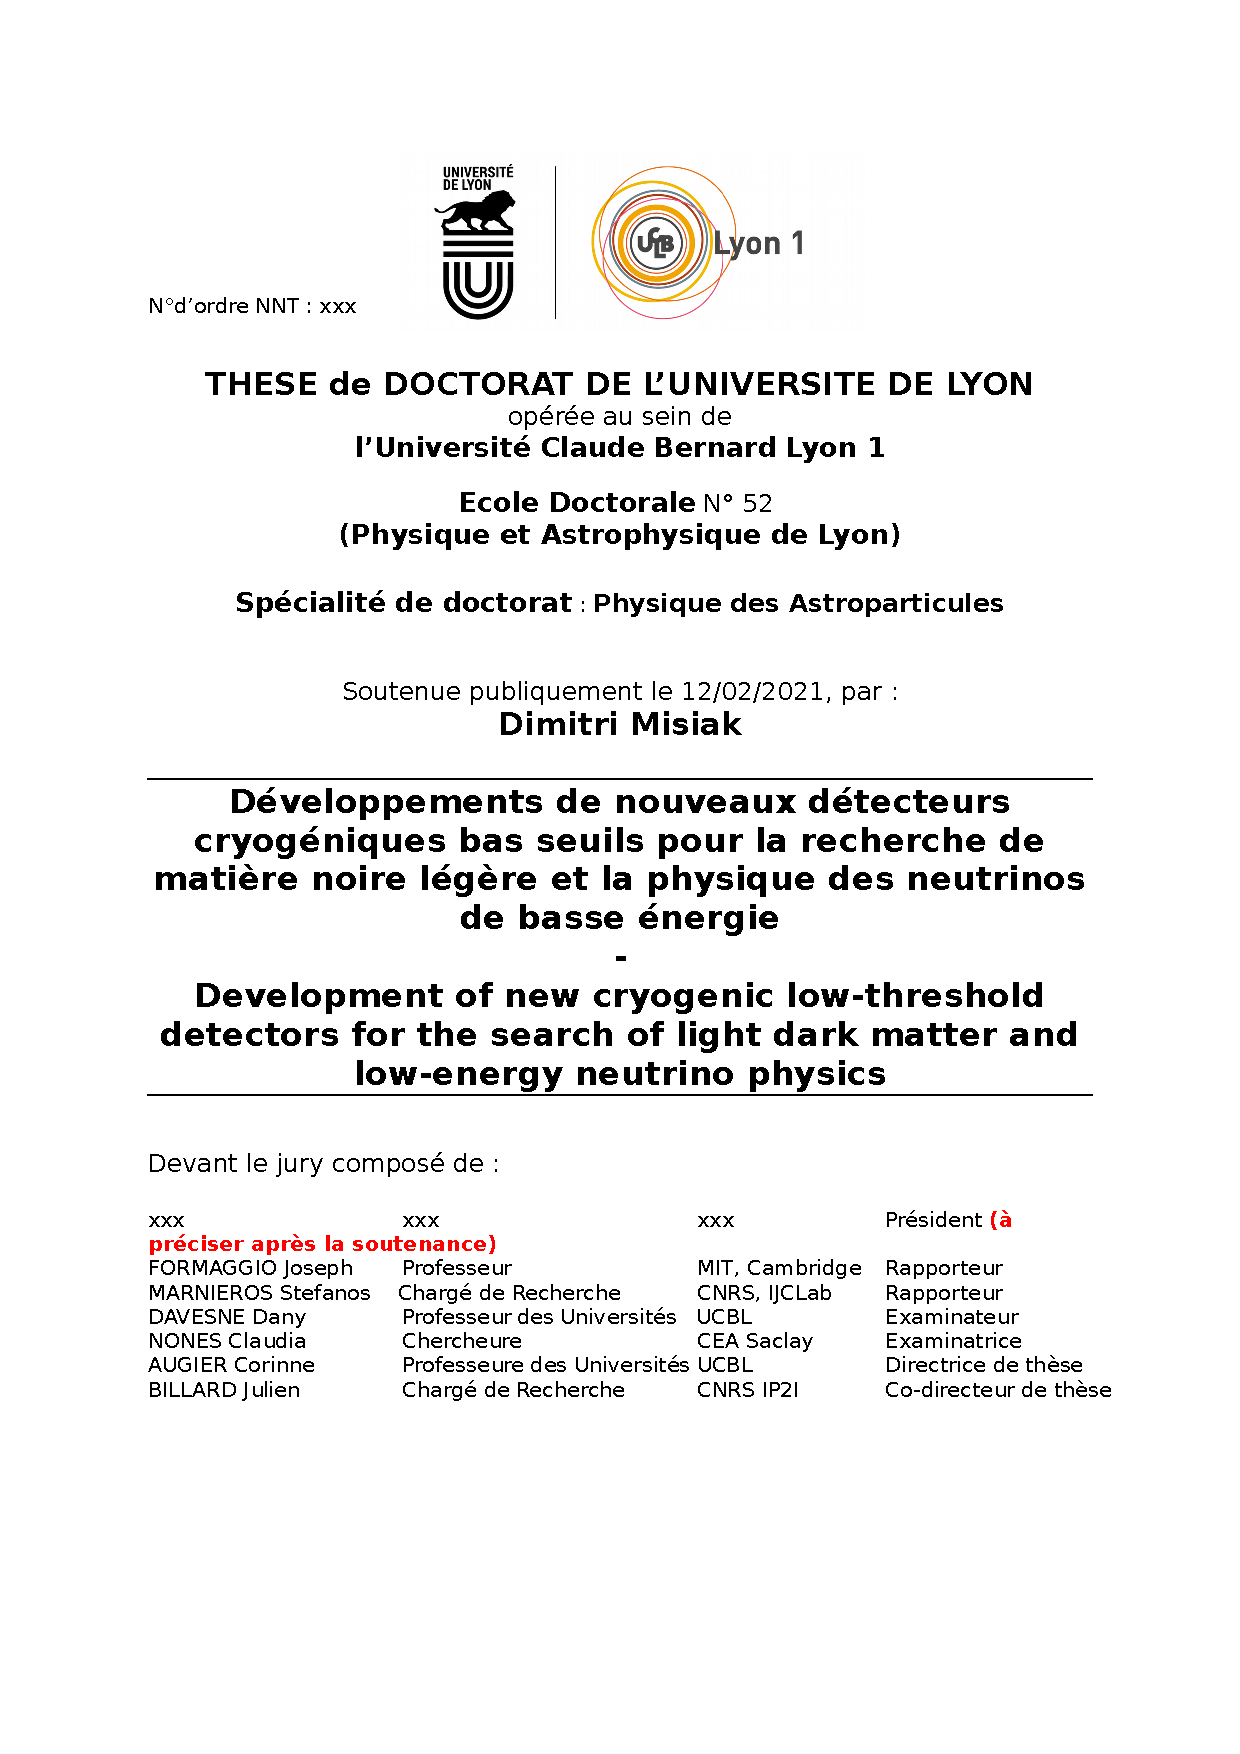
\includepdf[pages=-]{FrontPage/front_page.pdf}

%%%----------------------------------------------------------------------------------------
%%	TITLE PAGE
%%----------------------------------------------------------------------------------------
%
%\begin{titlepage}
%\begin{center}
%
%\vspace*{.06\textheight}
%{\scshape\LARGE \univname\par}\vspace{1.5cm} % University name
%\textsc{\Large Doctoral Thesis}\\[0.5cm] % Thesis type
%
%\HRule \\[0.4cm] % Horizontal line
%{\huge \bfseries \ttitle\par}\vspace{0.4cm} % Thesis title
%\HRule \\[1.5cm] % Horizontal line
% 
%\begin{minipage}[t]{0.4\textwidth}
%\begin{flushleft} \large
%\emph{Author:}\\
%\href{http://www.google.com}{\authorname} % Author name - remove the \href bracket to remove the link
%\end{flushleft}
%\end{minipage}
%\begin{minipage}[t]{0.4\textwidth}
%\begin{flushright} \large
%\emph{Supervisor:} \\
%\href{http://www.google.com}{\supname} % Supervisor name - remove the \href bracket to remove the link  
%\end{flushright}
%\end{minipage}\\[3cm]
% 
%\vfill
%
%\large \textit{A thesis submitted in fulfillment of the requirements\\ for the degree of \degreename}\\[0.3cm] % University requirement text
%\textit{in the}\\[0.4cm]
%\groupname\\\deptname\\[2cm] % Research group name and department name
% 
%\vfill
%
%{\large \today}\\[4cm] % Date
%\includegraphics{Logo} % University/department logo - uncomment to place it
% 
%\vfill
%\end{center}
%\end{titlepage}

%%%----------------------------------------------------------------------------------------
%%	DECLARATION PAGE
%%----------------------------------------------------------------------------------------
%
%\begin{declaration}
%\addchaptertocentry{\authorshipname} % Add the declaration to the table of contents
%\noindent I, \authorname, declare that this thesis titled, \enquote{\ttitle} and the work presented in it are my own. I confirm that:
%
%\begin{itemize} 
%\item This work was done wholly or mainly while in candidature for a research degree at this University.
%\item Where any part of this thesis has previously been submitted for a degree or any other qualification at this University or any other institution, this has been clearly stated.
%\item Where I have consulted the published work of others, this is always clearly attributed.
%\item Where I have quoted from the work of others, the source is always given. With the exception of such quotations, this thesis is entirely my own work.
%\item I have acknowledged all main sources of help.
%\item Where the thesis is based on work done by myself jointly with others, I have made clear exactly what was done by others and what I have contributed myself.\\
%\end{itemize}
% 
%\noindent Signed:\\
%\rule[0.5em]{25em}{0.5pt} % This prints a line for the signature
% 
%\noindent Date:\\
%\rule[0.5em]{25em}{0.5pt} % This prints a line to write the date
%\end{declaration}
%
%\cleardoublepage

%%----------------------------------------------------------------------------------------
%%	QUOTATION PAGE
%%----------------------------------------------------------------------------------------
%
%\vspace*{0.2\textheight}
%
%\noindent\enquote{\itshape INSERT FUNNY AND DEEP QUOTE HERE.}\bigbreak
%
%\hfill Famous Person or Obscure Reference

%%----------------------------------------------------------------------------------------
%%	ABSTRACT PAGE
%%----------------------------------------------------------------------------------------
%
%\begin{abstract}
%\addchaptertocentry{\abstractname} % Add the abstract to the table of contents
%
%{\small
%
%The Coherent Elastic Neutrino-Nucleus Scattering (CENNS) is a process predicted nearly 40 years ago. In August 2017, the COHERENT experiment reported the first keV-scale detection at the 6.7 sigma level of this process, which is a probe for the new low energy physics, opening a window on a myriad of new physics opportunities.
%
%The RICOCHET experiment aims at measuring with high accuracy the CENNS process in order to probe various exotic physics scenarios in the electroweak sector. Using cryogenic bolometers operated in a cryostat 8 meters away from the core of the ILL research nuclear reactor, the experiment will benefit from an intense neutrino flux, allowing the results of COHERENT to be reproduced in a single week. The objective of an accurate measurement will be achieved after one year of data collection, by 2024.
%The CRYOCUBE is a compact cubic array of cryogenic detectors with the following specifications: a very low energy threshold of $\mathcal{O}(10)$ eV on the thermal signal, an electromagnetic background rejection of at least $10^3$ and a total target mass of 1 kg distributed among 27 germanium crystals of about 30 g each.
%
%The objective of this thesis is to propose an optimized detector design for the CRYOCUBE, inspired by the cryogenic germanium detectors equipped with charge and temperature readings of the direct dark matter search experiment EDELWEISS. This joint R\&D program is based on event discrimination realized in germanium semiconductor crystals. The recoil energy of an incident particle is derived either from the increase of the crystal temperature measured by a GeNTD thermistor (heat channel) or from the excited electric charges collected by electrodes on its surface (ionization channel). This double energy measurement makes it possible to distinguish the nuclear recoils produced by the CENNS or the dark matter from the electronic radioactive background. As these recoils are of the order of $\mathcal{O}(100)$ eV, this thesis work is focused on the development of a new generation of cryogenic low threshold germanium detectors with particle identification. It explores how to improve the resolution in heat and ionization energy up to $\mathcal{O}(10)$ eV while maintaining a good rejection of background events. This study is based on the testing of prototype detectors in the IP2I cryostat, which are compared to theoretical predictions from electro-thermal and electrostatic modeling of the detectors.
%
%This manuscript begins with the definition of the CENNS process, its scientific importance and the objectives of the RICOCHET experiment. It then presents the cryogenic installation allowing the surface operation of the detectors at 20 mK in optimal conditions.
%An electro-thermal model of the bolometers, compared with experimental data, is developed and applied to the simulation of the noise associated with the electronics of the heat signal.
%The thesis then formalizes the generation of the ionization signals arising from excited charge carriers drifting in the germanium crystal under the influence of the applied electric field. The expected resolution from a future low-noise electronics is modeled based on two detector designs. They are optimized by their electrostatic simulation in a finite element calculation software. A comparison of the theoretical and experimental performance of ionization is performed on the basis of the RED80 and REDN1 prototype detectors.
%This work ends with the characterization of the radioactive background in the cryogenic laboratory with the analysis of the data from RED80, and in particular its neutron component, used to estimate the expected background at the ILL site for RICOCHET.
%
%}
%\end{abstract}
%
%
%\begin{abstractfr}
%\addchaptertocentry{\abstractnamefr} % Add the abstract to the table of contents
%
%{\small
%
%La diffusion élastique cohérente neutrino-noyau (CENNS) est un processus prédit il y a près de 40 ans. En août 2017, l'expérience COHERENT a rapporté la première détection à l’échelle du keV au niveau 6,7 sigma, de ce processus qui est une sonde pour la nouvelle physique à basse énergie, ouvrant une fenêtre sur une myriade de nouvelles possibilités en matière de physique.
%
%L'expérience RICOCHET vise à mesurer avec une grande précision le processus CENNS afin de sonder divers scénarios de physique exotique dans le secteur électrofaible. En utilisant des bolomètres cryogéniques installés dans un cryostat à 8 mètres du cœur du réacteur nucléaire de recherche de l'ILL, l’expérience bénéficiera d'un flux intense de neutrinos, permettant de reproduire les résultats de COHERENT en une semaine. L'objectif de mesure précise sera atteint après un an de collecte de données, d’ici 2024.
%Le CRYOCUBE est un ensemble compact cubique de détecteurs cryogéniques présentant les spécifications suivantes : un seuil en énergie très faible de $\mathcal{O}(10)$ eV sur le signal thermique, un rejet du fond électromagnétique d'au moins $10^3$ et une masse totale de la cible de 1 kg répartie entre 27 cristaux de germanium d'environ 30 g chacun.
%
%L'objectif de cette thèse est de proposer une conception optimisée des détecteurs pour le CRYOCUBE, inspirée des détecteurs cryogéniques en germanium équipés de lecture de charge et de températures de l'expérience de détection directe de matière noire EDELWEISS. Ce programme conjoint de R\&D est basé sur la discrimination d'événements réalisée dans des cristaux de germanium semi-conducteurs. L'énergie de recul d'une particule incidente est dérivée soit de l'augmentation de la température du cristal mesurée par une thermistance GeNTD (voie chaleur), soit des charges électriques excitées collectées par des électrodes à sa surface (voie ionisation). Cette double mesure d'énergie permet de distinguer les reculs nucléaires produits par le CENNS ou la matière noire, du fond radioactif électronique. Ces reculs étant de l’ordre de $\mathcal{O}(100)$ eV, ce travail de thèse est axé sur le développement d'une nouvelle génération de détecteurs cryogéniques au germanium à faible seuil avec identification des particules. Il explore comment améliorer la résolution en énergie chaleur et ionisation jusqu'à $\mathcal{O}(10)$ eV tout en conservant un bon rejet des événements de fond. Cette étude est basée sur l'essai de prototypes de détecteurs dans le cryostat IP2I, qui sont comparés aux prévisions théoriques issues de la modélisation électro-thermique et électrostatique des détecteurs.
%
%Ce manuscrit commence par la définition du processus CENNS, son importance scientifique et les objectifs de l'expérience RICOCHET. Il présente ensuite l'installation cryogénique permettant le fonctionnement en surface des détecteurs à 20 mK dans des conditions optimales.
%Un modèle électro-thermique des bolomètres, comparé à des données expérimentales, est développé et appliqué à la simulation du bruit associé à l’électronique du signal chaleur.
%La thèse formalise ensuite la génération des signaux d'ionisation résultant de la dérive, sous l'influence du champ électrique exercé, de porteurs de charge excités dans le cristal de germanium. La résolution attendue d’une future électronique bas-bruit est modélisée à partir de deux designs de détecteurs. Ils sont optimisés par leur simulation électrostatique dans un logiciel de calculs aux éléments finis. Une comparaison des performances théoriques et expérimentales de l'ionisation est effectuée sur la base des prototypes de détecteurs RED80 et REDN1.
%Ces travaux se terminent par la caractérisation du bruit de fond radioactif dans le laboratoire cryogénique avec l’analyse des données de RED80, et notamment sa composante neutronique, utilisée pour estimer le fond attendu sur le site ILL pour RICOCHET.
%
%}
%\end{abstractfr}


%%----------------------------------------------------------------------------------------
%%	ACKNOWLEDGEMENTS
%%----------------------------------------------------------------------------------------
%
%\begin{acknowledgements}
%\addchaptertocentry{\acknowledgementname} % Add the acknowledgements to the table of contents
%The acknowledgments and the people to thank go here, don't forget to include your project advisor\ldots
%\end{acknowledgements}

%----------------------------------------------------------------------------------------
%	LIST OF CONTENTS/FIGURES/TABLES PAGES
%----------------------------------------------------------------------------------------

\tableofcontents % Prints the main table of contents

%\listoffigures % Prints the list of figures

%\listoftables % Prints the list of tables

%%----------------------------------------------------------------------------------------
%%	ABBREVIATIONS
%%----------------------------------------------------------------------------------------
%
%\begin{abbreviations}{ll} % Include a list of abbreviations (a table of two columns)
%
%\textbf{PSD} & \textbf{P}ower \textbf{S}pectral \textbf{D}ensity \\
%\textbf{FID} & \textbf{F}ully \textbf{I}nter\textbf{D}igitized \\
%\textbf{NTD} & \textbf{N}eutron \textbf{T}ransmutation \textbf{D}oped \\
%\textbf{Ge} & \textbf{Ge}rmanium \\
%\textbf{RMS} & \textbf{R}oot \textbf{M}ean \textbf{S}quare \\
%\textbf{ADU} & \textbf{A}nalog-to-\textbf{D}igital conversion \textbf{U}nit \\
%\textbf{OF} & \textbf{O}ptimal \textbf{F}iltering \\
%
%\end{abbreviations}

%%----------------------------------------------------------------------------------------
%%	PHYSICAL CONSTANTS/OTHER DEFINITIONS
%%----------------------------------------------------------------------------------------
%
%\begin{constants}{lr@{${}={}$}l} % The list of physical constants is a three column table
%
%% The \SI{}{} command is provided by the siunitx package, see its documentation for instructions on how to use it
%
%Speed of Light & $c_{0}$ & \SI{2.99792458e8}{\meter\per\second} (exact)\\
%Boltzmann Constant & $k_B$ & \SI{1.380649e-23}{\joule\per\kelvin} (exact) \\
%Elementary Charge & $e$ & \SI{1.602176634e-19}{\coulomb} (exact)\\
%%Constant Name & $Symbol$ & $Constant Value$ with units\\
%
%\end{constants}

%%----------------------------------------------------------------------------------------
%%	SYMBOLS
%%----------------------------------------------------------------------------------------
%
%\begin{symbols}{lll} % Include a list of Symbols (a three column table)
%
%$T$ & temperature & \si{\kelvin} \\
%$P$ & power & \si{\watt} (\si{\joule\per\second}) \\
%$E$ & energy & \si{\joule} \\
%%Symbol & Name & Unit \\
%
%\addlinespace % Gap to separate the Roman symbols from the Greek
%
%$\omega$ & angular frequency & \si{\radian} \\
%
%\end{symbols}

%%----------------------------------------------------------------------------------------
%%	DEDICATION
%%----------------------------------------------------------------------------------------
%
%\dedicatory{For/Dedicated to/To my\ldots} 
%
%%----------------------------------------------------------------------------------------
%%	THESIS CONTENT - CHAPTERS
%%----------------------------------------------------------------------------------------

\mainmatter % Begin numeric (1,2,3...) page numbering

\pagestyle{thesis} % Return the page headers back to the "thesis" style

% Include the chapters of the thesis as separate files from the Chapters folder
% Uncomment the lines as you write the chapters

%% Introduction, Theory
%% Chapter Intro

\chapter{Low-threshold bolometers in Physics Experiments} % Main chapter title

\label{ChapterIntro} % Change X to a consecutive number; for referencing this chapter elsewhere, use \ref{ChapterX}

%----------------------------------------------------------------------------------------
%	BEGING CHAPTER
%----------------------------------------------------------------------------------------

\section{CE$\nu$NS and the new physics}

\subsection{Neutrino/core elastic coherent scattering}

A diffusion phenomenon occurs when two particles meet during a collsion. This report will focus in particular on the process of dissemination of the neutrinos with atomic nuclei. There are several particular cases of this diffusion: It is said to be elastic when the neutrino has not lost energy after having interacted with a nucleus (the direction of the neutrino is not necessarily preserved); coherent when the neutrino interacts with the nucleus as a whole in such a way that it is enough to consider the nucleus as a uniform object when it is known to be composed of nucleons. When the diffusion of a neutrino is coherent and elastic we speak of CE$\nu$NS (or CENNS) which is the acronym for Coherent Elastic Neutrino Nucleus Scattering. This physical phenomenon, described by Freedman in 1973 within the framework of the standard model, was experimentally measured for the first time in 2017 by the collaboration COHERENT installed near the spallation source at the Oak Ridge National Laboratory in the United States.
Before getting to the heart of the matter, it seems to me that it is essential to recall the various objects physical characteristics that will be discussed throughout this report in order to provide the non-specialist reader with the essential elements of understanding essential for the appreciation of the scientific context of my work. We will therefore discuss atomic nuclei, neutrinos, the CEvNS equations and of the various experiments aimed at measuring it.


\subsection{The atomic nucleus}

Rutherford's experience with gold leaf in 1909 provided valuable information for the development of Bohr's atomic model in 1913. Rutherford understood that the electrically positively charged of an atom is concentrated in the middle of the atom. Indeed, knowing that the matter is electrically neutral and that an atom has electrons 1 (charged negatively) there are necessarily positive charges "somewhere". Bohr then designed a atomic model for hydrogen that reminds us of a planetary system. There would be the nucleus at center and the electrons around it, only allowed to be on specific circular orbitals.
Theoretical and experimental developments show us today that the electrons are not really on circular orbits but rather have a probability of presence described by combinations of spherical harmonics. Bohr's model for hydrogen is not fundamentally questioned and is still taught. With the boom in scientific communication over the last few decades, everyone knows today that every atom has a nucleus and that its charge is positive. The latter can be either stable or unstable in the case of radioactive elements. 
This is an important fact, that an atom is not a fundamental object of modern physics: it is composed of nucleons (neutrons and protons), which are themselves composed of three quarks held together by
to the strong nuclear interaction mediated by gluon. The size of an atom is of the order of
of 0.1 nm (10 -10 m), in comparison the nucleus is only a femtometer (10 -15 m). The nucleus
is one hundred thousand times smaller than the atom it is composed of.


\subsection{The neutrino}

The neutrino is one of the elementary particles of the Standard Model of Party Physics. Technically it is said to be an electrically neutral lepton. There are three flavors of neutrinos associated respectively with the electron $e^-$ , the muon $\mu^-$ and the tau $\tau^-$ : the electronic, muonic and tauic neutrino.
The physicist Wolfgang Pauli was the first to postulate the existence of the neutrino in 1930. This new particle (at the time) helped to explain the continuous spectrum of the beta disintegration, which is a radioactive reaction in which a radionucleide emits an electron (or positron) and an (anti-)neutrino.
The experimental confirmation will be made in 1952 by Cowan and Queens based on an idea by Wang Ganchang (1942), the first two were awarded the Nobel Prize for physics in 1995 for this discovery.
A neutrino is only sensitive to the weak nuclear force and gravity, which is negligible most of the time. Due to the short range of the weak interaction (10 -18 m) the neutrino has a very low probability of interaction with matter, in physics we speak of an weak cross-section. To have an order of magnitude in mind we can show that out of 10 billion neutrinos of 1MeV that cross the earth, only 1 will interact with matter. I would like to warn the reader that in this report no particular attention will be brought on distinction between neutrinos and anti-neutrinos as well as different flavors. The reason is that the neutrino-nucleus elastic coherent diffusion process is insensitive to these differences.


\subsection{CENNS and standard model}

It was in 1973 that Daniel Z. Freedman, a physicist currently at MIT, proposed the coherent elastic neutrino-nucleus scattering as a probe for weak interaction [2]. In its description based on the standard particle physics model still under development at the time (it will take its current form in the mid-1970s) Freedman expresses the evolution rate of the effective cross section of the neutrino-nucleus interaction as a function of the recoil energy of the nucleus.core bottom (1.1). This equation shows that the evolution of the effective cross-section noted $\sigma(E_{\nu} , \sigma{E_r} )$ depends on the neutrino energy $E_{\nu}$ and recoil energy $E_r$ of the nucleusas well as
of the mass of the target nucleus $m_A$ and its composition $(N ,Z)$.

\begin{equation}
\frac{\mathrm{d} \sigma (E_{\nu}, E_r)}{\mathrm{d} E_r}
=
\frac{G_{f}^2}{4\pi}
Q_w^2  m_A
\left( 1 - \frac{m_A E_r}{2 E_{\nu}^2} \right)
F^2(E_r)
\end{equation}

Without going into the details of the theoretical calculations to obtain this expression, one can try to explain simply the terms that seem the most technical

The Fermi coupling constant is measured experimentally by studying life time of the muon (inversely proportional to $G_f^2$) [3]. We can express this constant as a function of the coupling constant of the weak interaction $g_W$ , the mass $m_W$ of the boson W, the speed of light $c$ and the reduced Planck constant $\hbar$ according to the equation (1.2).
\begin{equation}
G_f 
=
\frac{\sqrt{2}}{8}
\left( \frac{g_W}{m_W c^2} \right)^2
(\hbar c)^3
\sim \SI{1.17e-5}{\giga \eV^-2}
\end{equation}

The weak nuclear hypercharge $Q_w$ given by (1.3) shows the mixing angle $\theta_w$ which is a parameter of the Weinberg-Salam theory of the electr-weak interaction (reunification of the theory of electromagnetism and weak interaction).
\begin{equation}
Q_w = N - Z (1 - 4 \sin^2 \theta_w)
\end{equation}

The value of $\sin^2 \theta_w$ is close to 0.24 [4] which leads, in practice, to $Q_w \simeq N$. As described later in this work, the measurement of the $\sin^2 \theta_w$ as a function of the transferred momentum would permit to probe for new physic.

The shape factor $F$ is a function of the recoil energy that characterizes the loss of coherence at high transferred momentum. It is worth 1 for low recoil energies, so it is often neglected in very low energy regimes, and decreases with $E_r$.

We can also show [5], by integrating (1.1) from $E_r = 0$ to $E_r^{max} = 2E_{\nu}^2 / (m_A + 2E_{\nu} )$, the maximum recoil energy of the nucleus accessible for a given neutrino energy $E_{\nu}$, that the effective (total) cross-section is proportional to the square of the number of neutrons $N$ in the target nucleus and the energy of the neutrino thanks to the coherence of the interaction in case $m_N \gg E_{\nu}$ :
\begin{equation}
\sigma
\sim
\frac{G_f^2 N^2}{4\pi} E_{\nu}^2
\end{equation}

The CENNS event rate, $R$, is directly related to the differential cross-section of the scattering process through the relationship (1.5). The detection of CENNS is not done by directly measuring the cross-section of the particles that interact with the atomic nuclei of the detector. We measure the number of neutrinos having interacted with a nucleus according to the recoil energy of the latter. By doing this on a fairly wide range of recoil energy, we end up with what is called a energy spectrum of CENNS events. In this case, we will speak of CENNS spectrum, and of energy spectrum in the general case for different scattering processes. The expected CENNS event rate $R$ is calculated from the cross-section (1.5) by convolving with the incoming neutrino flux $\Phi$:
\begin{equation}
\frac{\mathrm{d} R}{\mathrm{d} E_r}
=
\mathcal{N} \cdot
\int_{E_{\nu}^{min}}
\Phi(E_{\nu})
\cdot
\frac{\mathrm{d} \sigma (E_{\nu}, E_r) }{\mathrm{d} E_r} \mathrm{d} E_{\nu}
\end{equation}

In this equation, $\mathcal{N}$ represents the number of target nuclei per mass unit. The minimum energy of a neutrino to induce a nuclear recoil is given by the relation $E_{\nu}^{min}= \sqrt{m_N E_r /2}$.

A common representation of this type of interaction in particle physics is done with the help of Feynman diagrams. In this representation, the time flows from left to right and the distance between the particles is represented along the vertical axis. The mediator bosons are indicated with wavy lines. The Feynman diagram of the CENNS is given by the scheme presented in Figure \ref{fig:cenns-feynman}, where the $Z_0$ boson is the mediator of the weak interaction in the usual standard model framework on the left or within the framework of an alternative theory on the right.

\begin{figure}
\centering
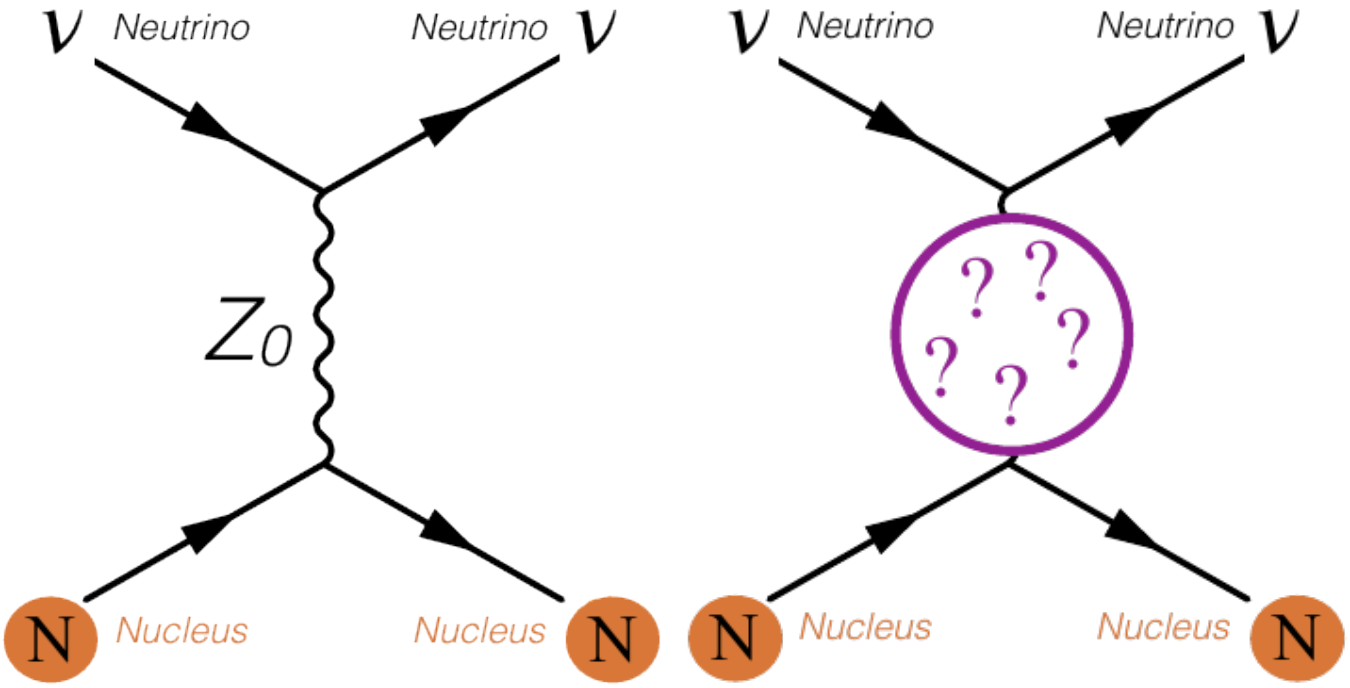
\includegraphics [scale=1]{Figures/Introduction/cenns_feynman.png}
\caption{Feynman diagram of the CEvNS. On the left in the case of the standard model. To the right
the same process within the framework of alternative theories (symbolic representation).}
\label{fig:cenns-feynman}
\end{figure}


\subsection{First detection of CEvNS}

The COHERENT collaboration was the first to observe experimentally and unambiguously the signature of the CENNS in 2017 [6]. The technology used at that time was a \SI{14.6}{\kg} sodium-doped cesium iodide (\ce{CsI[Na]}) scintillator instrumented with photo-multipliers. The detector was located at a distance of \SI{19.3}{\m} from the neutrino source and had an energy detection threshold of \SI{4.5}{\kilo\eV}. The neutrino flux of average energy $E_{\nu} = \SI{30}{\mega\eV}$ used for this detection was produced with the so-called "pion-at-rest" method presented in figure 1.2. It consists in taking advantage of the decay of positive pawns, obtained after a controlled collision of a mercury atom with a proton, which leads to the production of neutrinos and anti-neutrinos. The proton source comes from the SNS (Spallation Neutron Source) located at the Oak Ridge National Laboratory in Oak Ridge, Tennessee (USA). 

Scientists in the collaboration have detected an excess of CENNS-related events, shown in Figure \ref{fig:coherent-result}, with a confidence of $6.7\sigma$ compatible at $1\sigma$ with the standard model. The uncertainty of the statistical study they estimate is \SI{16}{\percent}. This first detection of CENNS is a result which proves the existence of this phenomenon which has been considered for years by some as purely hypothetical. It has made it possible to constrain models of new physics [6] but the current data do not allow to study the theories expected in the lower energies such as the existence of new mediating bosons [7]. This requires a source of lower energy neutrinos.

\begin{figure}
\centering
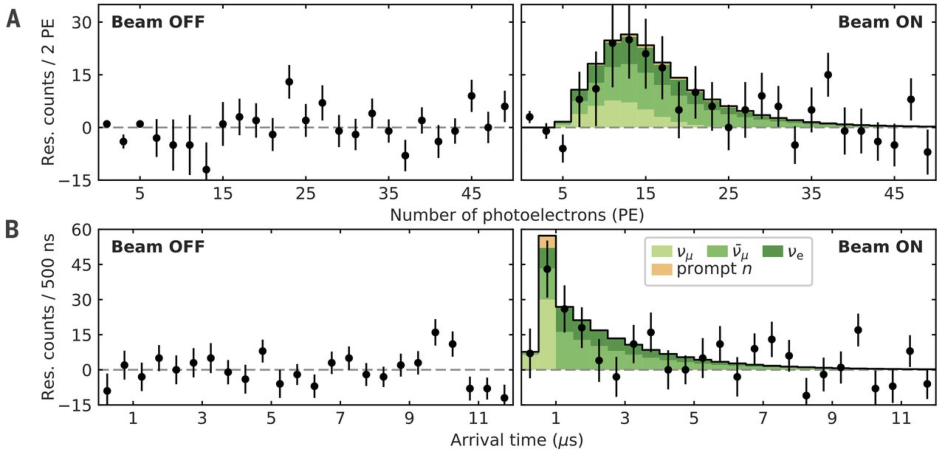
\includegraphics [scale=1]{Figures/Introduction/coherent_result.pdf}
\caption{Experimental result of the COHERENT experiment at the SNS demonstrating unambiguously
the existence of the CEvNS.}
\label{fig:coherent-result}
\end{figure}


\section{Search for new low energy physics}

A number of theories diverge significantly from the model's prediction low energy standard. Among them we can mention in particular :
\begin{itemize}
	\item The existence of new \ce{Z_0} mediator bosons.
	\item The existence of an abnormally high magnetic moment of the neutrino.
	\item The existence of non-standard interactions.
\end{itemize}

There is an important scientific stake in making these low energy measurements to provide additional elements in the understanding of fundamental interactions but also to provide additional constraints for a large number of neutrino research projects. A precise measurement of the CENNS would, for example, make it possible to constrain theoretical models. 

However, to do new physics research with the CENNS process requires the use of a suitable neutrino source. This source must meet two fundamental criteria:
\begin{itemize}
	\item Produce a very high flux of neutrinos, the higher the flux the greater the mass of the detector may be low at an equivalent CENNS event rate.
	\item Have a known and adapted neutrino energy spectrum (typically $E_{\nu} \approx \SI{10}{\mega\eV}$).
\end{itemize}
Then, various technical and practical considerations are taken into account: possibility of interruption of the flow (or pulsed flow) for background rejection (as in the case of COHERENT for example), minimum accessible source/detector distance (the closer you are to the source, the closer you are to the detector) the greater the flow of neutrinos), ease of access and installation, regulations and availability of infrastructure.

\subsection{Neutrino sources}

There are many sources of neutrinos because the decay processes that generate them are very common in nature. We will discuss here some neutrino sources and their characteristics for CEvNS physics. Neutrinos out of experimental range such as those composing the neutrino diffuse background (the analogue of the neutrino diffuse cosmological background for neutrinos) will not be discussed. The resting pion method used by COHERENT will not be recalled as it has already been presented and is not a viable solution for the search for new low energy physics because of the too large energy of the emitted neutrinos.

\subsubsection{Solar neutrinos}

Thermonuclear fusion reactions take place in the heart of stars. During these reactions, low energy neutrinos (a few \si{\mega\eV}) are emitted. They escape from their original star without great difficulty thanks to their low effective cross-section. The responsible process of \SI{85}{\percent} of the neutrinos of our star, the sun, is the fusion of two protons \ce{p} (1.6) which gives a \ce{^2H} deuterium (heavy hydrogen) nucleus, an anti-electron \ce{e^+} (otherwise known as positron) and an electronic neutrino \ce{\nu_e}.
\begin{equation}
\ce{ p + p -> {}^2H + e^+ + $\nu$_e }
\end{equation}
For this specific reaction the energy of the emitted neutrinos is approximately of the order of of the hundred or so \si{kilo\eV}. It should be noted, however, that there are other reactions of a different nature producing neutrinos within the sun. For your information, the spectrum of solar neutrinos seen from the ground is shown in Figure \ref{fig:solar-neutrino-spectrum}. Taking all energies together, from the Earth, the flux of solar neutrinos is of the order of \SI{7e10}{\cm^{-2} \s^{-1}} which is relatively small and makes the detection of solar neutrinos very difficult.

\begin{figure}
\begin{minipage}{0.48\textwidth}
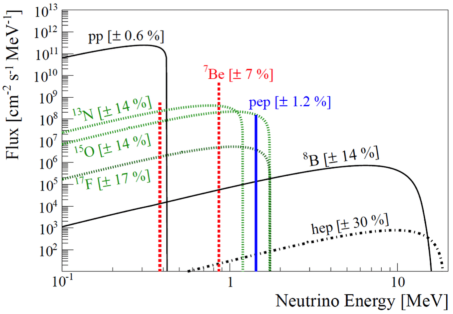
\includegraphics [scale=1]{Figures/Introduction/solar_neutrino_spectrum_simu.pdf}
\end{minipage}
\hfill
\begin{minipage}{0.48\textwidth}
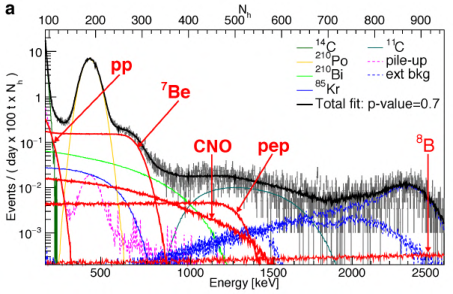
\includegraphics [scale=1]{Figures/Introduction/solar_neutrino_spectrum_exp.pdf}
\end{minipage}
\caption{Solar neutrino spectrum. Left Simulated spectrum of solar neutrinos seen from
the earth [1]. At right Solar neutrino spectrum measured by the Borexino experiment.
at the Gran Sasso in Italy.}
\label{fig:solar-neutrino-spectrum}
\end{figure}

Despite this difficulty, large experiments such as Borexino, located in the underground laboratory of the Gran Sasso in Italy, are able to measure them (see Figure \ref{fig:solar-neutrino-spectrum}). However, for a CENNS precision measurement experiment the sun is clearly not a relevant source because even if the energy of some neutrinos is low enough for probing new physics, it is not a relevant source of energy as the flow remains far too low and would require a huge volume (mass) of detector. Another negative point is that it is not possible to turn off the source to identify the background noise. Indeed, even at night the neutrinos cross the earth without difficulty.

\subsubsection{Terrestrial neutrinos (geo-neutrinos)}

Planet Earth emits neutrinos through natural radioactivity processes. Neutrinos resulting from these radioactive processes are numerous, it is estimated [8] that the flow of neutrinos of origin geologic surface of the earth around \SI{1e6}{\cm^{-2} \s^{-1}}. With such a low flux (and a wide energy distribution) they are very difficult to detect because of the background of neutrinos of extraterrestrial and human origin. Nevertheless some experiments try to carry out geo-neutrino measurements for the information they would allow us to obtain on the Earth and in particular at the level of the Earth's core. The members of Borexino (still them) claim to have recently detected 53 events attributable to geo-neutrinos [9]. For reasons similar to solar neutrinos, geo-neutrinos are not relevant in view of the current knowledge for CENNS precision measurement.

\subsubsection{Production from Human Activity}

Humans are capable of producing neutrinos in controlled physical processes. In particle accelerators, for example, it is not uncommon to produce neutrinos with energies of up to \SI{100}{\giga\eV}. But these are the nuclear fission power plants which are the most intense source of low-energy neutrinos. Neutrinos are produced in power generation plants without this being the main objective. They are in a way a very abundant by-product. The flow of neutrinos emitted by a standard nuclear power plant \SI{10}{\m} from the reactor is approximately equal to \SI{2e15}{\cm^{-2} \s^{-1}}, for an average neutrino energy of \SI{4}{\mega\eV}. Nuclear fission reactors offer a range of energy compatible with the research of new physics as envisioned by RICOCHET, the neutrino flux is among the most important and in addition to that it is possible to take advantage of unit outages to measure background noise. For this last point the subtraction background noise is not as optimal as with a pulsed source if the background noise is not stationary on the time scales represented by the combustion of a fuel rod but it is always an interesting plus to gain in measurement accuracy.


\subsection{Reactor experiments}

The strong potential of nuclear power plants as sources of neutrinos has led a small number of CEvNS experiments to be installed close to a reactor core around the world, the experiments that I have been able to identify are shown in Figure 1.5 and a short description of each of them is given in Table 1.1.

\begin{figure}
\centering
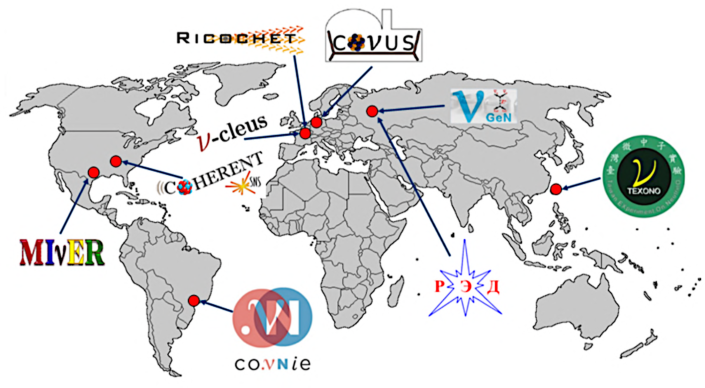
\includegraphics[scale=1]{Figures/Introduction/cenns_exp_atlas.pdf}
\caption{Main experiences of CEvNS in the world today (2020).}
\label{fig:cenns-exp-atlas}
\end{figure}

\begin{table}[]
\centering
\begin{tabular}{c|c|c}
Experiment & (Detector Material) @ Location & Reference  \\ \hline \hline
NuGEN & 	(Ge) @ Kalinin Reactor (Russie) &	[10] \\
CONUS & 	(Ge) @ Brokdorf (Allemagne) &	[11] \\
TEXONO & 	(Ge) @ Kuo-Sheng Reactor (Taiwan) &	[12] \\
CONNIE & 	(Si) @ Angra Reactor (Brésil) &	[13] \\
RED100 & 	(Xe) @ Kalinin Reactor (Russie) &	[14] \\
MINER & 	(GeSi) @ Nuclear Science Center (USA) &	[15] \\
NU-CLEUS &	(\ce{CaWO_4}, \ce{Al_2O_3} ) @ Chooz (France) &	[16] \\
RICOCHET & 	(Ge, Zn, Al, (Si)) @ ILL (France) &	[17] \\
\end{tabular}
\caption{Presentation of CENNS experiments associated with a nuclear reactor: materials used for detection @ localization. In red are represented the cryogenic experiments with a very low detection threshold for the research of new physics. The RICOCHET experiment is the only one to propose a detector capable of discriminating between nuclear and electronic recoils.}
\label{tab:reactor-experiments}
\end{table}

The CEvNS experiments near a reactor would allow us to estimate the Weinberg angle at low energies. Figure \ref{fig:weinberg-angle} shows the prediction of the standard model (blue line) for this parameter and the zone of the parameter space accessible by the CEvNS experiments (green zone) which still remains largely unexplored. The estimation of this parameter with different physical processes is also very important to identify incompatibilities and allow us to go beyond the current theoretical model.

\begin{figure}
\centering
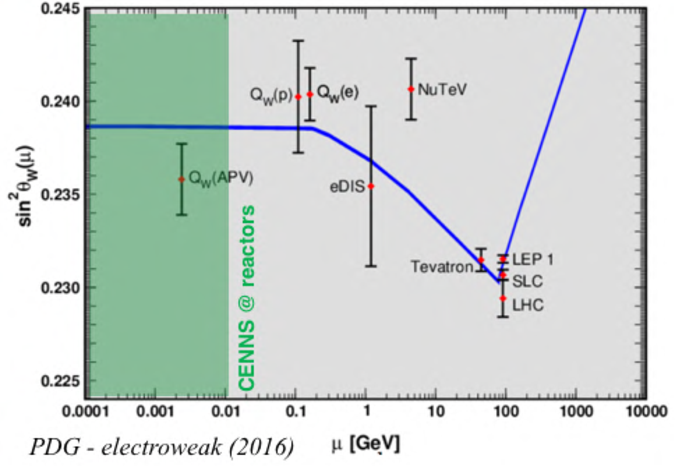
\includegraphics[scale=1]{Figures/Introduction/weinberg_angle.pdf}
\caption{Measurements of the Weinberg angle as a function of the impulse (or transferred moment). In
blue we have the prediction of the standard model for different processes and experiments. In
green shows the area accessible by the CEvNS near a nuclear reactor.}
\label{fig:weinberg-angle}
\end{figure}

In view of the number of CEvNS experiments we can expect scientific results showing deviations (or not) from the standard low energy model within a few years only. The "cooperation" at work between all these collaborations and with dark matter experiments such as EDELWEISS favors rapid developments and technological improvements.


\subsection{RICOCHET}

RICOCHET is a CENNS experience led by the members of the MANOIR team at the IP2I of Lyon, which brings together some fifty researchers, technicians and engineers through various laboratories and universities in France, Russia and the United States. RICOCHET aims at to measure the CENNS spectrum with a statistical accuracy of \SI{1}{\percent} after one year of taking data and to detect CENNS with low energy neutrinos (a few \si{\mega\eV}) with an accuracy of $5\sigma$ in only a few days of operation. 
It should be noted that the targeted accuracy is far superior to that obtained by COHERENT. To achieve these scientific objectives the RICOCHET device is composed of a cryogenic system, a shielding to limit sources of unwanted noise and the CRYOCUBE detector. It will be installed in 2022 at the Laue Institute Langevin (ILL, Grenoble), where a \SI{58}{\mega\watt} fission research nuclear reactor is located. A numerical modeling of RICOCHET at ILL and the implementation scheme near the reactor core are visible in figure \ref{fig:ricochet-ill-site}.

\begin{figure}
\centering
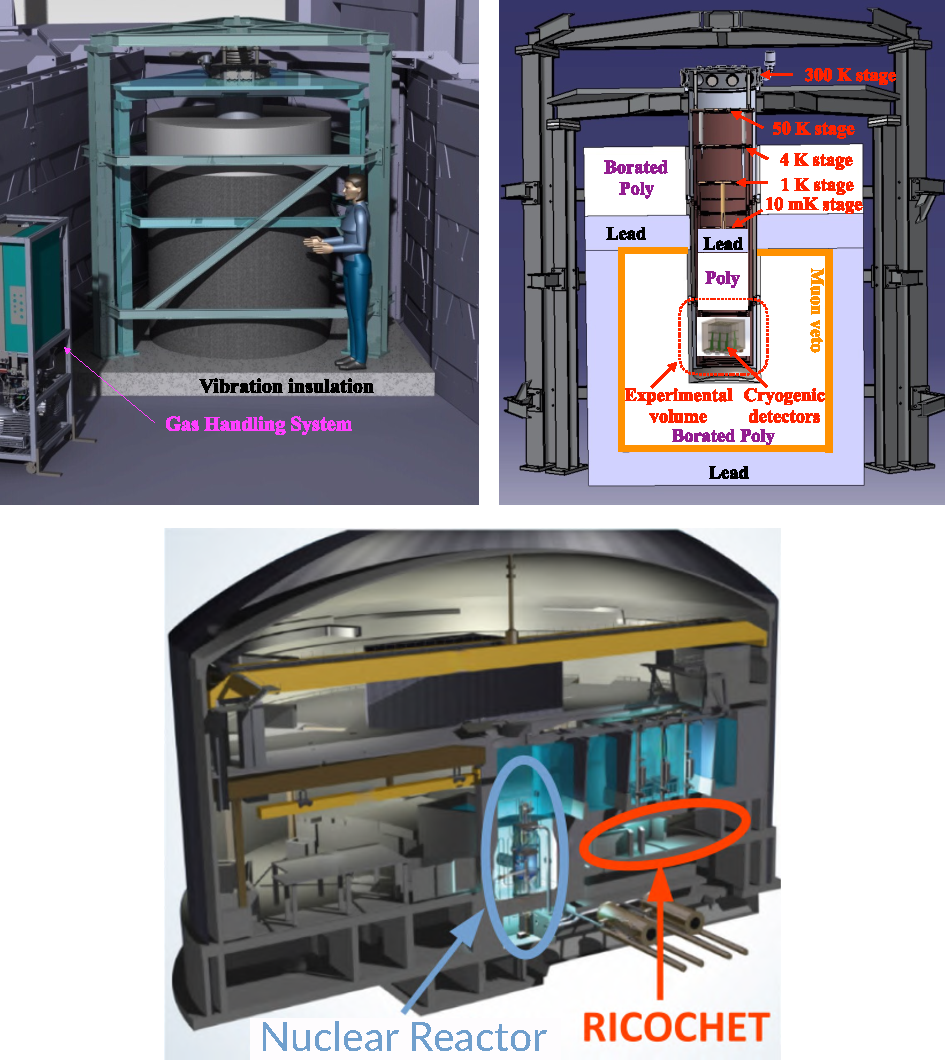
\includegraphics[scale=1]{Figures/Introduction/ricochet_ill_site.pdf}
\caption{On the top left Installation of RICOCHET at ILL, 3D modeling. On the top right, View in
cryostat cut. At the bottom, location of the RICOCHET cryostat within the ILL nuclear reactor. The water pool above the location of RICOCHET provides protection against cosmic particles.}
\label{fig:ricochet-ill-site}
\end{figure}

The CRYOCUBE detector will be at only \SI{8}{\m} from the core of the nuclear reactor with a power of \SI{58}{\mega\watt} which will produce a neutrino flux of \SI{e12}{\cm^{-2} \s^{-1}}. The CRYOCUBE will be cool down a cryogenic temperature of only a few thousandths of a degree above absolute zero, between 5 and \SI{20}{\milli\kelvin}, in order to be able to measure minute temperature rises caused by the neutrinos during their interaction with the nuclei that make up the detector's target material.

The operation of the CRYOCUBE detector will be detailed later. But it is necessary to know that this detector will be protected from external radiation by a thick layer of shielding of more than 15 tons and an active cosmic particle rejection device called veto muon. The objective being to free itself as much as possible from all unwanted diffusion processes. and thus increase the signal-to-noise ratio and, indeed, the chances of being able to detect signs of new physics.

At the precise location of RICOCHET at the ILL, the incident neutrino flux is known and
the Manoir team has precisely simulated the expected CENNS spectrum according to different theoretical models considered and taking into account the different background noises. On this figure \ref{fig:cenns-new-physics} we see the prediction of the standard model (in blue) and the assumed effect of two alternative theories: the existence of an abnormally high neutrino moment (violet, fine dotted line) or of a new particular Z' boson (violet, dashed line). The background noise, of electronic or nuclear origin, is represented in grey and is both almost uniform in the energy range considered.

This numerical simulation allows to define a specification for a ca CENNS spectrum can be measured specifically in the region of interest for the new physical. Intuitively, we can see that we need a detection threshold in energy enough otherwise we will not be able to see the deviations from the standard model or even the CENNS itself by the way!

\begin{figure}
\centering
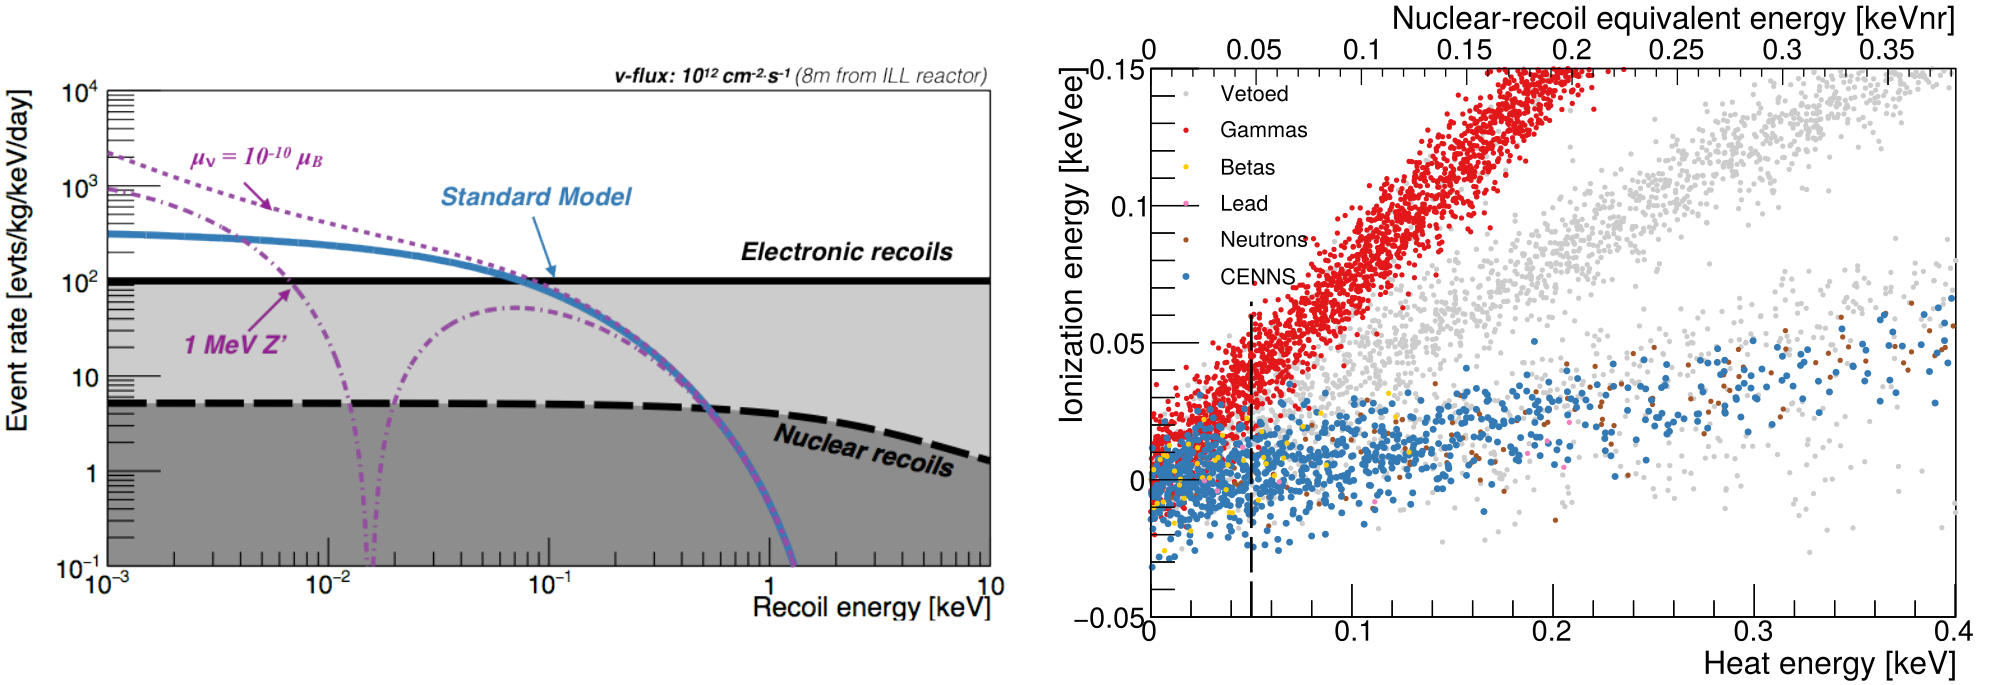
\includegraphics[scale=1]{Figures/Introduction/cenns_new_physics.png}
\caption{Left Simulation of the background noise on the CENNS spectrum for RICOCHET at the ILL : background noise of electronic recoils (light grey). Background noise of nuclear retreats (dark gray). At right Discrimination of nuclear (blue) and electronic (red) retreats
by simultaneous measurement of ionization and heat. (simulation)}
\label{fig:cenns-new-physics}
\end{figure}

We can notice that the spectrum is given in \si{events \per \kilo\eV \per \kg \per \day} and therefore to have a sufficient statistic it is necessary to find an interesting ratio detector mass over data acquisition time. Indeed having an ultra massive detector represents a real technical challenge. One can quote for example the dark matter research experiment XENON1T which uses a detector whose total mass is greater than one ton and its version in development XENONnT which aims to go even further in terms of mass.  This detector technology, based on a liquefied noble gas, is not the most efficient for the CENNS but above all requires a large experimental volume that is difficult to obtain near a nuclear reactor. Other technologies such as super-K or Borexino experiments would be theoretically possible but the experimental volume would remain an impossible constraint to reconcile with the proximity of a nuclear reactor. The opposite approach would consist in taking a low detector mass (easy to install, easy to analyze, easy to protect from external pollution) and waiting a long time. In theory there would be no problem to but in practice the non-stationarity of the noise, the volume of the data, the time to analyze this data and the time of experience (mobilization of human resources, technical, infrastructure, ...) make the task very difficult. There is therefore a compromise to between the mass of the detector and the desired duration of data acquisition for a given number of CENNS events.

The exposure (mass multiplied by the experiment time) of the detector is not the only parameter to be considered, it is necessary to have sufficient sensitivity to measure the minute variations in temperature generated by the interaction of a neutrino with matter and to be able to differentiate between nuclear and electronic recoils in order to increase the signal-to-noise ratio (as suggested by numerical simulation). To carry out this identification of neutrino recoils, one way to do this is to measure the temperature increase induced by a deposit of energy while measuring the electron-hole pairs created in the semiconductor material that serves as a target for coherent elastic scattering. The ratio between the number of pairs created and the temperature rise is different for an electronic recoil and for a nuclear recoil as shown in the simulation on the right in figure \ref{fig:cryocube} where we see the nuclear recoils in blue and the electronic recoils in red. It is therefore necessary to measure both the temperature and the temperature rise. ionization in the material to be able to differentiate between the two types of interaction.

Specifically, a detector with the following characteristics would be required:
\begin{itemize}
	\item Detection threshold / energy resolution: $E_R \sim \SI{50}{\eV}$ / $\sigma(E_R) \sim \SI{10}{\eV}$
	\item Ability to discriminate between electronic and nuclear recoil with thermometer + electrodes for electronic noise rejection with semiconductor material 
	\item Mass of the detector: $m_d \sim \SI{1}{\kg}$ with a flux of \SI{e12}{\cm^{-2} \s^{-1}} to have about ten of CENNS events per day
\end{itemize}

To meet these specifications, the members of the RICOCHET collaboration are developing an innovative detector called CRYOCUBE which is presented in the figure \ref{fig:cryocube}. It will be composed of 27 germanium crystals of \SI{38}{\g} so as to provide a heat measurement and four ionizations per crystal for discrimination. The energy threshold
of \SI{50}{\eV} on the heat path has already been demonstrated with the RED20 prototype.

\begin{figure}
\centering
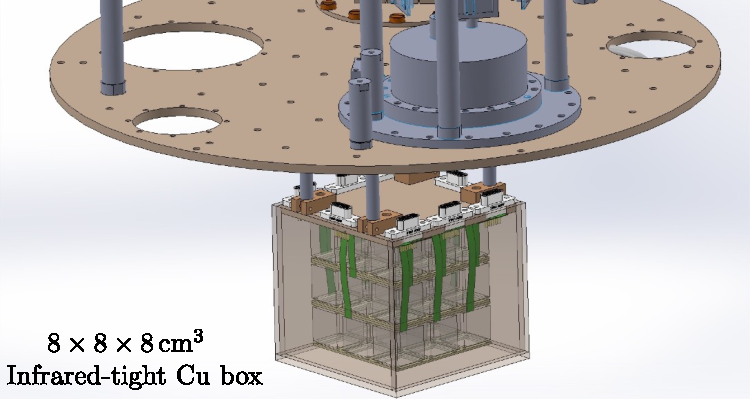
\includegraphics[scale=1]{Figures/Introduction/cryocube.pdf}
\caption{3D model of the CRYOCUBE installed in its cryostat. We can see by transparency the 27 germanium crystals of 38g electrically connected to the systems
of acquisition by the green cables.
}
\label{fig:cryocube}
\end{figure}


RICOCHET is a relatively large scientific experiment that requires good project management. The implementation of the CRYOCUBE technology, through the joint development program RICOCHET and EDELWEISS on RED detectors is a very expensive step. For information, each 30g germanium crystal costs about ten thousand euros because of the requirements of purity and geometry (polishing, ...). One understands the need to deepen the approach and optimization on single crystal detectors before building the final CRYOCUBE. The CRYOCUBE project is supported by an ERC starting grant awarded to Julien Billard, IP2I researcher. The cryostat to host the CRYOCUBE is custom-built by the French company CryoConcept and financed by our Russian collaborators to the tune of five hundred thousand euros, to which must be added shielding, electronics, computer systems and human resources costs. Excluding human resources, RICOCHET's installation at ILL is estimated at more than three million euros (all funding combined: ANR, ERC, laboratories, ...).



%\section{Theoretical Objectives}
%
%The R\&D team of the MANOIR group is developing cryogenic bolometers for the search of low energy chargeless particles. Its work contributes to the EDELWEISS and the RICOCHET experiments.
%
%The EDELWEISS is a direct dark matter search experiment. The dark matter problem emerges from discrepancies between cosmological observations and theoretical expectations (galaxies spinning faster than expected from their luminous masses for example). Even though there is a lot of theories (MACHO, modified gravitation, etc...) which could explain these differences, the favorite is the existence of a Weakly Interacting Massive Particle (WIMP). This particle is non relativist, chargeless and rarely interact with ordinary matter. According to cosmological constraints, WIMP particles forms a halo/cloud comprising our galaxy, meaning that this particles are present and could be detected on Earth.
%
%The RICOCHET is a neutrino experiment for the precise measurement of the Coherent Elastic Neutrino-Nucleus Scattering (CENNS). Predicted in the 70s, this process was only discovered in 2017 thanks to modern technology. The study of this process at low energy level could unravel new physics but this calls for very sensitive neutrino detectors. Coincidentally, dark matter detectors are well-adapted to the challenges of the CENNS measurement although few adjustments and a proximity to a neutrino source (like a nuclear reactor) are needed.
%
%\section*{Introduction}
%
%The problem of dark matter has been motivating many physicists in the fields of cosmology, astrophysics and particle physics for several decades. Various cosmological observations have indeed proved the presence of non-visible mass in the universe, and thus created one of the major challenges of modern physics. The great emulation present in this field of study has given birth to many scientific collaborations, and with them, many experiments for the research of dark matter.
%
%It is in this scientific context that I carried out my second year Master's internship within the Manor Group of the IPNL whose work is part of the EDELWEISS collaboration. She is working on a direct detection experiment located in the Laboratoire Souterrain de Modane under the Fréjus tunnel. Recently reconverted in the search for light dark matter, the collaboration is relaunching a research and development campaign to obtain detectors with low energy detection thresholds.
%
%This report describes the development work on cryogenic detectors that I carried out during 4 months. I had the opportunity to perform experimental data acquisition on the IPNL R\&D crysotat, to develop theoretical tools for detector modeling and to compare the modeling with the experimental measurement.
%The first part of the report is devoted to a reminder of the dark matter problem, and to the description of the detection principle used in the detectors of the EDELWEISS experiment. In a second part, the two detectors studied (RED1 and RED10) are presented and an electro-thermal model is built. The third part gathers the different experimental results. There is first a characterization of the electronics with the RED1 detector, then a thermal characterization of RED10 with comparison to the electro-thermal model. We will finish with the preliminary optimization results using all the results presented in this report.
%
%\section*{Introduction}
%
%
%\section{The detection of light dark matter within EDELWEISS}
%
%\subsection{Dark matter evidence}
%
%There is evidence of the existence of dark matter at several scales. At the cosmological scale, for example, it is the latest measurements from the PLANCK \cite{planck} collaboration that provide an energy-matter composition of the universe. This would be composed of only $4\%$ of baryonic matter while dark matter would represent $26.1\%$. On a rather local scale, we have the work of Vera Rubin who has highlighted this dark matter by studying the distribution of velocities within spiral galaxies. A curve of the velocity of the stars as a function of their distance from the galactic center is presented in figure \ref{galaxy}.
%
%\begin{figure}[!ht]
%\begin{center}
%\includegraphics [scale=1]{Images/curve_rot.pdf}
%\end{center}
%\caption{The velocities of the stars in the spiral galaxy are represented according to their distance from the galactic center. The measured velocity curve (in black) is compared to the one simulated (in green) from the measured luminous mass. The red curve corresponds to the velocity curve of the dark matter halo potential. Figure from \cite{spiral}.}.
%\label{galaxy}.
%\end{figure}
%
%The experimental measurements (in black) are compared with the velocity curve calculated from the luminous mass of the galaxy (in red). The velocity curve does not decrease with the distance contrary to the prediction, but remains constant. To explain this, it is necessary to add to the model the presence of a massive and non-luminous halo encompassing the luminous matter (in green), this would be the famous dark matter.
%
%
%\subsection{Introduction of the WIMP candidate}
%
%Several hypotheses about dark matter have already been put forward. The idea that dark matter can be made of baryonic objects such as black holes or brown dwarfs is discarded. Indeed, the MACHO (MAssive Compact Halo Object) and Eros experiments have shown that such objects could not explain more than $10%$ of the observed dark matter contribution. We therefore converge towards a model where dark matter is made of particles. Another hypothesis proposing neutrinos as a candidate comes up against the scenario of formation of the structures of the universe. This so-called "bottom-up" scenario, where small structures are precursors to large ones, indicates the non-relativity of dark matter particles, called cold dark matter.
% 
%Numerous observations have allowed to draw up an inventory of the constraints that dark matter must respect. The most likely candidate for dark matter, respecting at best these constraints, is the WIMP (Weakly Massive Interacting Particle). It is a particle:
%\begin{itemize}
%\item Massive and non-relativistic, with a mass of between $1$Gev and $1$TeV,
%\item Neutral electrical load, therefore not subject to electromagnetic interaction,
%\item neutral in color, therefore not subject to strong interaction,
%\item interacting by low interaction with a very low effective section,
%\item detectable from a terrestrial laboratory, its flux is estimated at about $10^5$WIMPs/cm${}^2$/s.
%\end{itemize}
%
%\subsection{Dark matter detection methods}
%
%The search for dark matter is therefore equivalent to searching for WIMPs. There are three detection methods illustrated in figure \ref{3way} :
%\begin{itemize}
%\item Indirect detection is equivalent to observing the possible annihilation product of two dark matter particles that would then produce observable standard model particles, such as neutrinos, gamma radiation, or antimatter.
%\item Production is equivalent to studying Standard Model particle collision processes in collider-type experiments such as the Large Hadron Collider. A loss of energy in the energy balance could be explained by the production of dark matter that would escape the detectors.
%\item Direct detection is the study of the elastic collision between a WIMP and a target nucleus. The measurement of the recoil energy deposited by the WIMP allows to deduce its mass as well as the effective cross-section of the interaction process.
%\end{itemize}
%
%\begin{figure}[!ht]
%\begin{minipage}{0.49\textwidth}
%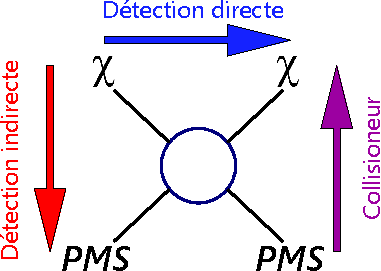
\includegraphics [width=\textwidth]{Images/direct_detection.pdf}
%\end{minipage}
%\hfill
%\vrule{}
%\hfill
%\begin{minipage}{0.40\textwidth}
%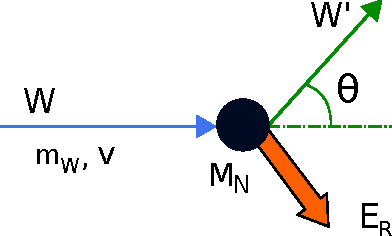
\includegraphics [width=\textwidth]{Images/wimp_diff.pdf}
%\end{minipage}
%\hfill
%\caption{(left) Graphical representation of the different methods of dark matter detection. $\chi$ designates a dark matter particle and $PMS$ designates a standard model particle. \\
%(right) Representative scheme of the elastic collision of a WIMP, noted \textbf{W}, on a kernel, \textbf{N}. The WIMP then transfers a recoil energy $E_R$ to the kernel.}
%\label{3way}
%\end{figure}
%
%These three detection channels are complementary. Indeed, each method observes the interaction diagram of figure \ref{3way} in a different way. As the analysis of the experimental results depends on the model used, it is first necessary to make hypotheses about this model (standard model, supersymmetry or even more exotic ...). It is then possible to compare the results and further constrain the search for dark matter.
%
%The EDELWEISS collaboration is working on a direct detection experiment. Indeed, predictions of stellar dynamics assert that the WIMP flux on Earth is intense enough to hope to detect them. For this, the elastic scattering process is used on target nuclei of the so-called absorber part of the detector as shown in figure \ref{3way}. The recoil energy $E_R$ supplied to the absorber part of the detector is expressed and detected as :
%\begin{itemize}
%\item scintillation, we measure the photons coming from the de-excitation of the absorber atoms,
%\In ionization, electron-hole pairs for a solid absorber or electron-ion pairs for a gas/liquid absorber created during the collision are collected by applying an electric field,
%\item heat, phonons are emitted into the absorber and relax to create a measurable temperature rise.
%\end{itemize}
%The recoil energy fractions for each expression pathway depend on the physical characteristics of the particle interacting with the detector, as well as on the material composing the detector. In general, a material used in a detector allows to channel this recoil energy into only two energy expression pathways. The double measurement of these two forms of expression allows an active discrimination of the observed particles. In the case of EDELWEISS, the absorber is a germanium crystal which allows the expression of the recoil energy in the form of ionization and heat.
%
%The WIMP interacts with the nucleus via the weak interaction providing it with recoil energy $E_R$ with a certain interaction cross section $\sigma_{\chi + n \rightarrow \chi + n}$. A direct detection experiment thus allows to probe the mass space, deduced from the recoil energy, and the effective cross sections, deduced from the event statistics. By gathering the results of all the direct detection experiments, we obtain the state of the art diagram presented in figure \ref{art}.
%
%
%\begin{figure}[!ht]
%\begin{center}
%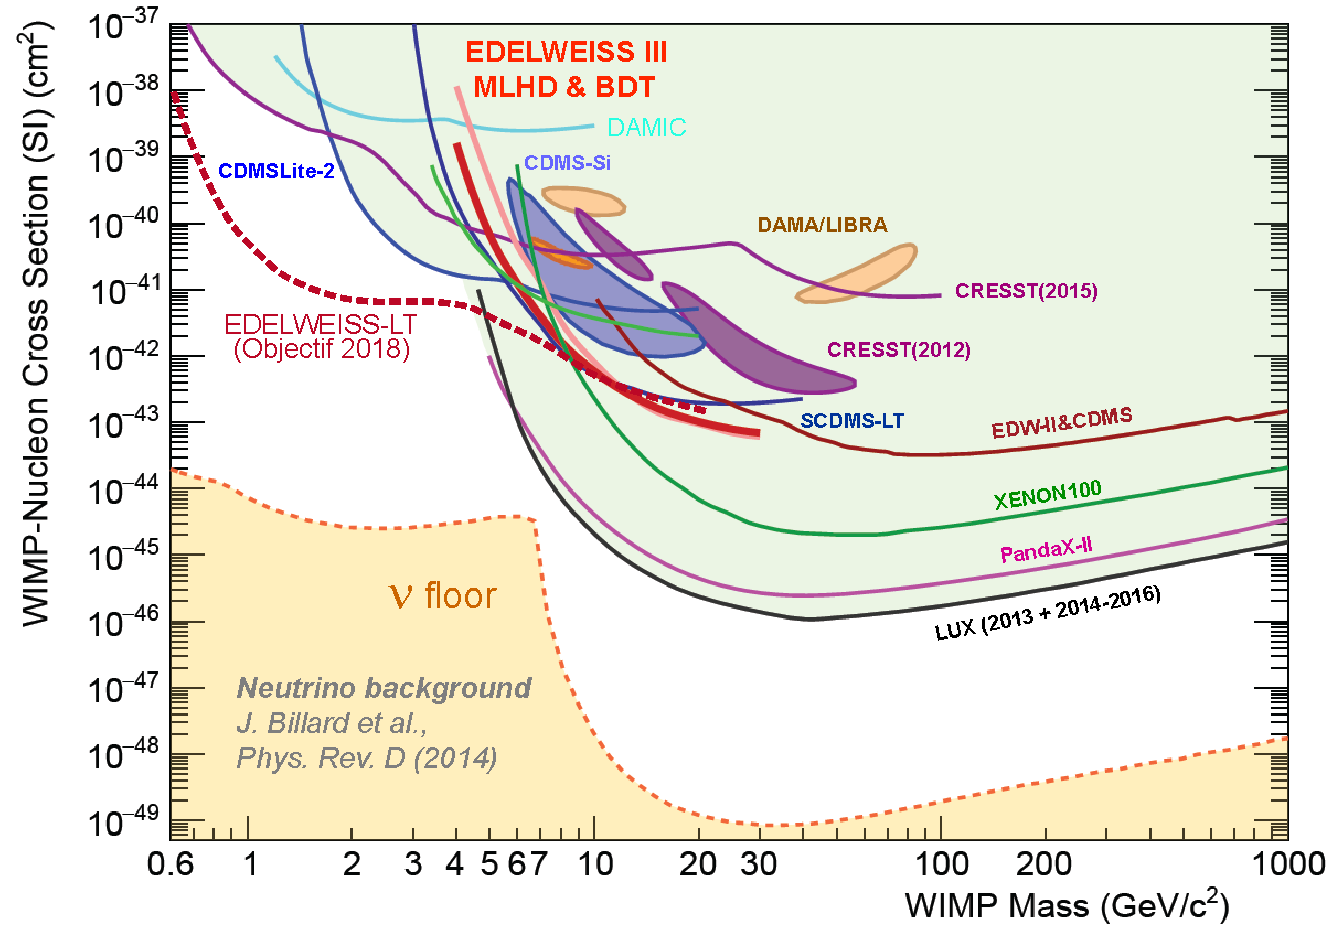
\includegraphics[width=0.75\textwidth]{Images/stateofart.pdf}
%\end{center}
%\caption[]{
%Diagramme de l'état de l'art pour la détection directe de WIMP. Dans l'espace de masse du WIMP et de la section efficace d'interaction WIMP-nucléon, il est représenté :
%%\begin{itemize}
%%\item en traits pleins : les courbes d'exclusions, chacune associée à une expérience de détection,
%%\item en bleu : l'espace déjà sondé et exclu,
%%\item en blanc : l'espace restant à être sondé,
%%\item en orange : limite de détection directe fixée par les neutrinos cosmiques,
%%\item les contours colorés : détections possibles de WIMPs, cependant exclues par d'autres résultats négatifs,
%%\item courbe rouge pointillée : objectif de la collaboration EDELWEISS pour 2018.
%%\end{itemize}
%}
%\label{art}
%\end{figure}
%\section*{Introduction}
%
%
%This diagram allows to visualize the exclusion curves drawn by the different collaborations, the space already surveyed, the intrinsic limit to direct detection set by cosmic neutrinos, and the space still to be surveyed. The latter is divided into two zones. The first concerns high mass WIMPs ($>10 GeV$) which deliver high recoil energy at the cost of a very low interaction cross section. Probing this area requires very massive detectors that can accumulate large exposures. The second area concerns low mass WIMPs ($<10 GeV$): this is the research area of EDELWEISS. The effective cross section is higher, so there is less concern about exposure. Nevertheless, the mass being small, the deposited recoil energy is also low. It is therefore necessary to work with detectors whose energy detection threshold is sufficiently small. The objective of the EDELWEISS collaboration for the year 2018 is a new exclusion curve (drawn in red dashes on the figure \ref{art}) requiring the development of a detector fulfilling the "$4\times 100$" objective described below.
%
%\subsection{The EDELWEISS experiment and the $4\times 100$} objective
%
%The name EDELWEISS stands for Experience for Detecting Underground WIMPs.
%This experiment uses cryogenic detectors in a cryostat that allows the temperature to drop down to $18mK$ and a very high vacuum. Direct detection with low energy detection threshold requires to reduce to the maximum any source of noise. 
%
%This is why the cryostat containing the detectors is placed within a shielding of layers of lead (including archaeological lead) and polyethylene to reduce as much as possible the impact of gamma radiation from the ambient radioactivity and the surrounding neutron background, respectively. This shielding is itself surrounded by a muon detection device called a "muon veto" which allows active discrimination of muons because they can produce neutrons in the detector enclosure. Finally, the EDELWEISS experiment is carried out in the Modane Underground Laboratory, in the middle of the Fréjus Tunnel, sheltered by more than $1700$m of rock. This natural barrier reduces the flow of cosmic muons by a factor of 6, which gives favorable conditions for direct detection with low energy thresholds.
%
%The detectors used by the EDELWEISS collaboration aim to measure the recoil energy deposited as ionization and heat. The objective 2018 to obtain a new exclusion curve requires the development of a new generation of detectors. The energy detection threshold must be increased from $2$keV to $100$eV. To do this, the objective "$4\times 100$" must be met:
%\begin{itemize}
%\item 100 Volts of voltage applied to the absorber. The charges created by ionization contribute to increase the heat signal by the Luke effect by drifting towards the collection electrodes. Increasing the voltage is equivalent to amplifying the heat signal.
%\item 100 eV resolution in ionization. 
%\A 100-fold decrease in heat-only events. These are non-ionizing background noise events that prevent the detection of a potential WIMP signal.
%\item 100 eV resolution in heat channel.
%\end{itemize}
%The first three points have been obtained or are in the process of being obtained. Only the improvement of the heat path remains necessary to meet the "$4\times 100$" objective and thus draw a new exclusion curve. 
%
%My internship work is part of the EDELWEISS R\&D campaign to improve the energy resolution of the heat channel of its detectors. A series of simplified "RED" detectors has been created for this purpose.
%The objective of my internship is to study the designs of the detectors, to build a complete thermal model of the detectors, to characterize the electronic noise of the detectors and finally to start the optimization process.



% Experimental Set-up
%% Chapter Experiment

\chapter{Experimental Setup at the IP2I cryogenic facility} % Main chapter title

\label{ChapterExperiment} % Change X to a consecutive number; for referencing this chapter elsewhere, use \ref{ChapterX}

%----------------------------------------------------------------------------------------
%	BEGING CHAPTER
%----------------------------------------------------------------------------------------

This chapter describes the IP2I Cryostat Facility in which the cryogenic germanium detectors presented in this work were operated. It explains how cryogenic conditions are obtained, presents the cryogenic germanium detectors and their principle of operation.

\section{The IP2I cryogenic facility}
\label{sec:IP2I-cryostat-facility} 

% Intro
The particle detectors studied in this work are cryogenic germanium bolometers. The term "cryogenic" indicates that these detectors are operated at cryogenic temperatures below $\SI{1}{\kelvin} = \SI{-272,15}{\celsius}$. In order to reach such temperatures, the detectors are placed inside of a \ce{^3He}/\ce{^4He} dilution cryostat.

The experimental results discussed in this work were obtained by running germanium detectors in the the dry dilution cryostat of the \textit{Institut de Physique des 2 Infinis de Lyon} (IP2I). The IP2I cryogenic facility is located in the basement of the IP2I Haefely building (see figure \ref{fig:haefely-building}). With an almost negligible overburden roughly estimated to be about \SI{1.5}{m.w.e} (meter water equivalent), the cryogenic detectors are operated in an above-ground (or surface) experiment as opposed to the underground operation of the \Edelweiss{} detectors at the LSM.

% Radioactive shielding
In order to reduce the environmental gamma background, the cryostat is surrounded by a \SI{10}{\cm} thick cylindrical lead shield covering a solid angle of $\sim \SI{70}{\percent}$ of $4\pi$ around the detectors. A reduction of about a factor of 10 is estimated on the triggering rate of our detectors with this lead shield.
There is no lead shield inside the cryostat. The materials used for the cryostat construction were not selected for low radioactivity, with the exception of the replacement of the standard glass fiber rods \footnote{used by the Cryoconcept company which built the cryostat} by stainless steel ones, shown to have much less radioactive contamination. 
While the radioactive background is high as a consequence of the above-ground operation, it is very similar to what is expected from the ILL site for the \Ricochet{} experiment. The neutron and gamma components of this background are characterized down to \SI{1}{\kilo\eV} in Chapter \ref{ChapterNeutron}.

\begin{figure}
\centering
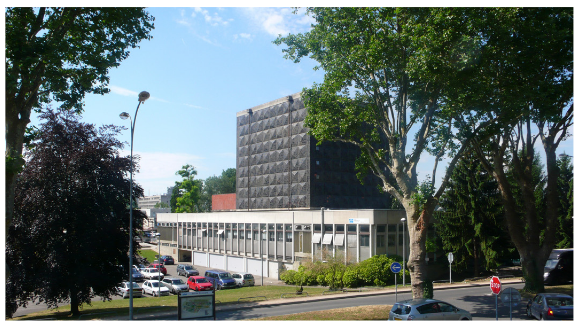
\includegraphics[width=\textwidth,angle=0]{Figures/Experiment/haefely_building.png}
\caption{Photo of the IP2I Haefely building. The cryogenic facility is located in the basement, at the same height as the parking lot.}
\label{fig:haefely-building}
\end{figure}

The total surface area of the facility is about a \SI{100}{\m^2} and encompasses the main cryogenic lab (\SI{80}{\m^2}), a technical room for pumps and gas handling system (\SI{6}{\m^2}), an ISO-5 clean room for detector mounting (\SI{9}{\m^2}), and a room hosting a chemical bench also related to detector fabrication (\SI{5}{\m^2}). A photo of the cryogenic laboratory is displayed in figure \ref{fig:cryolab} with the open cryostat in the corner of the room next to the lead shield on the left and the acquisition electronics and computers on the right.

\begin{figure}
\begin{center}
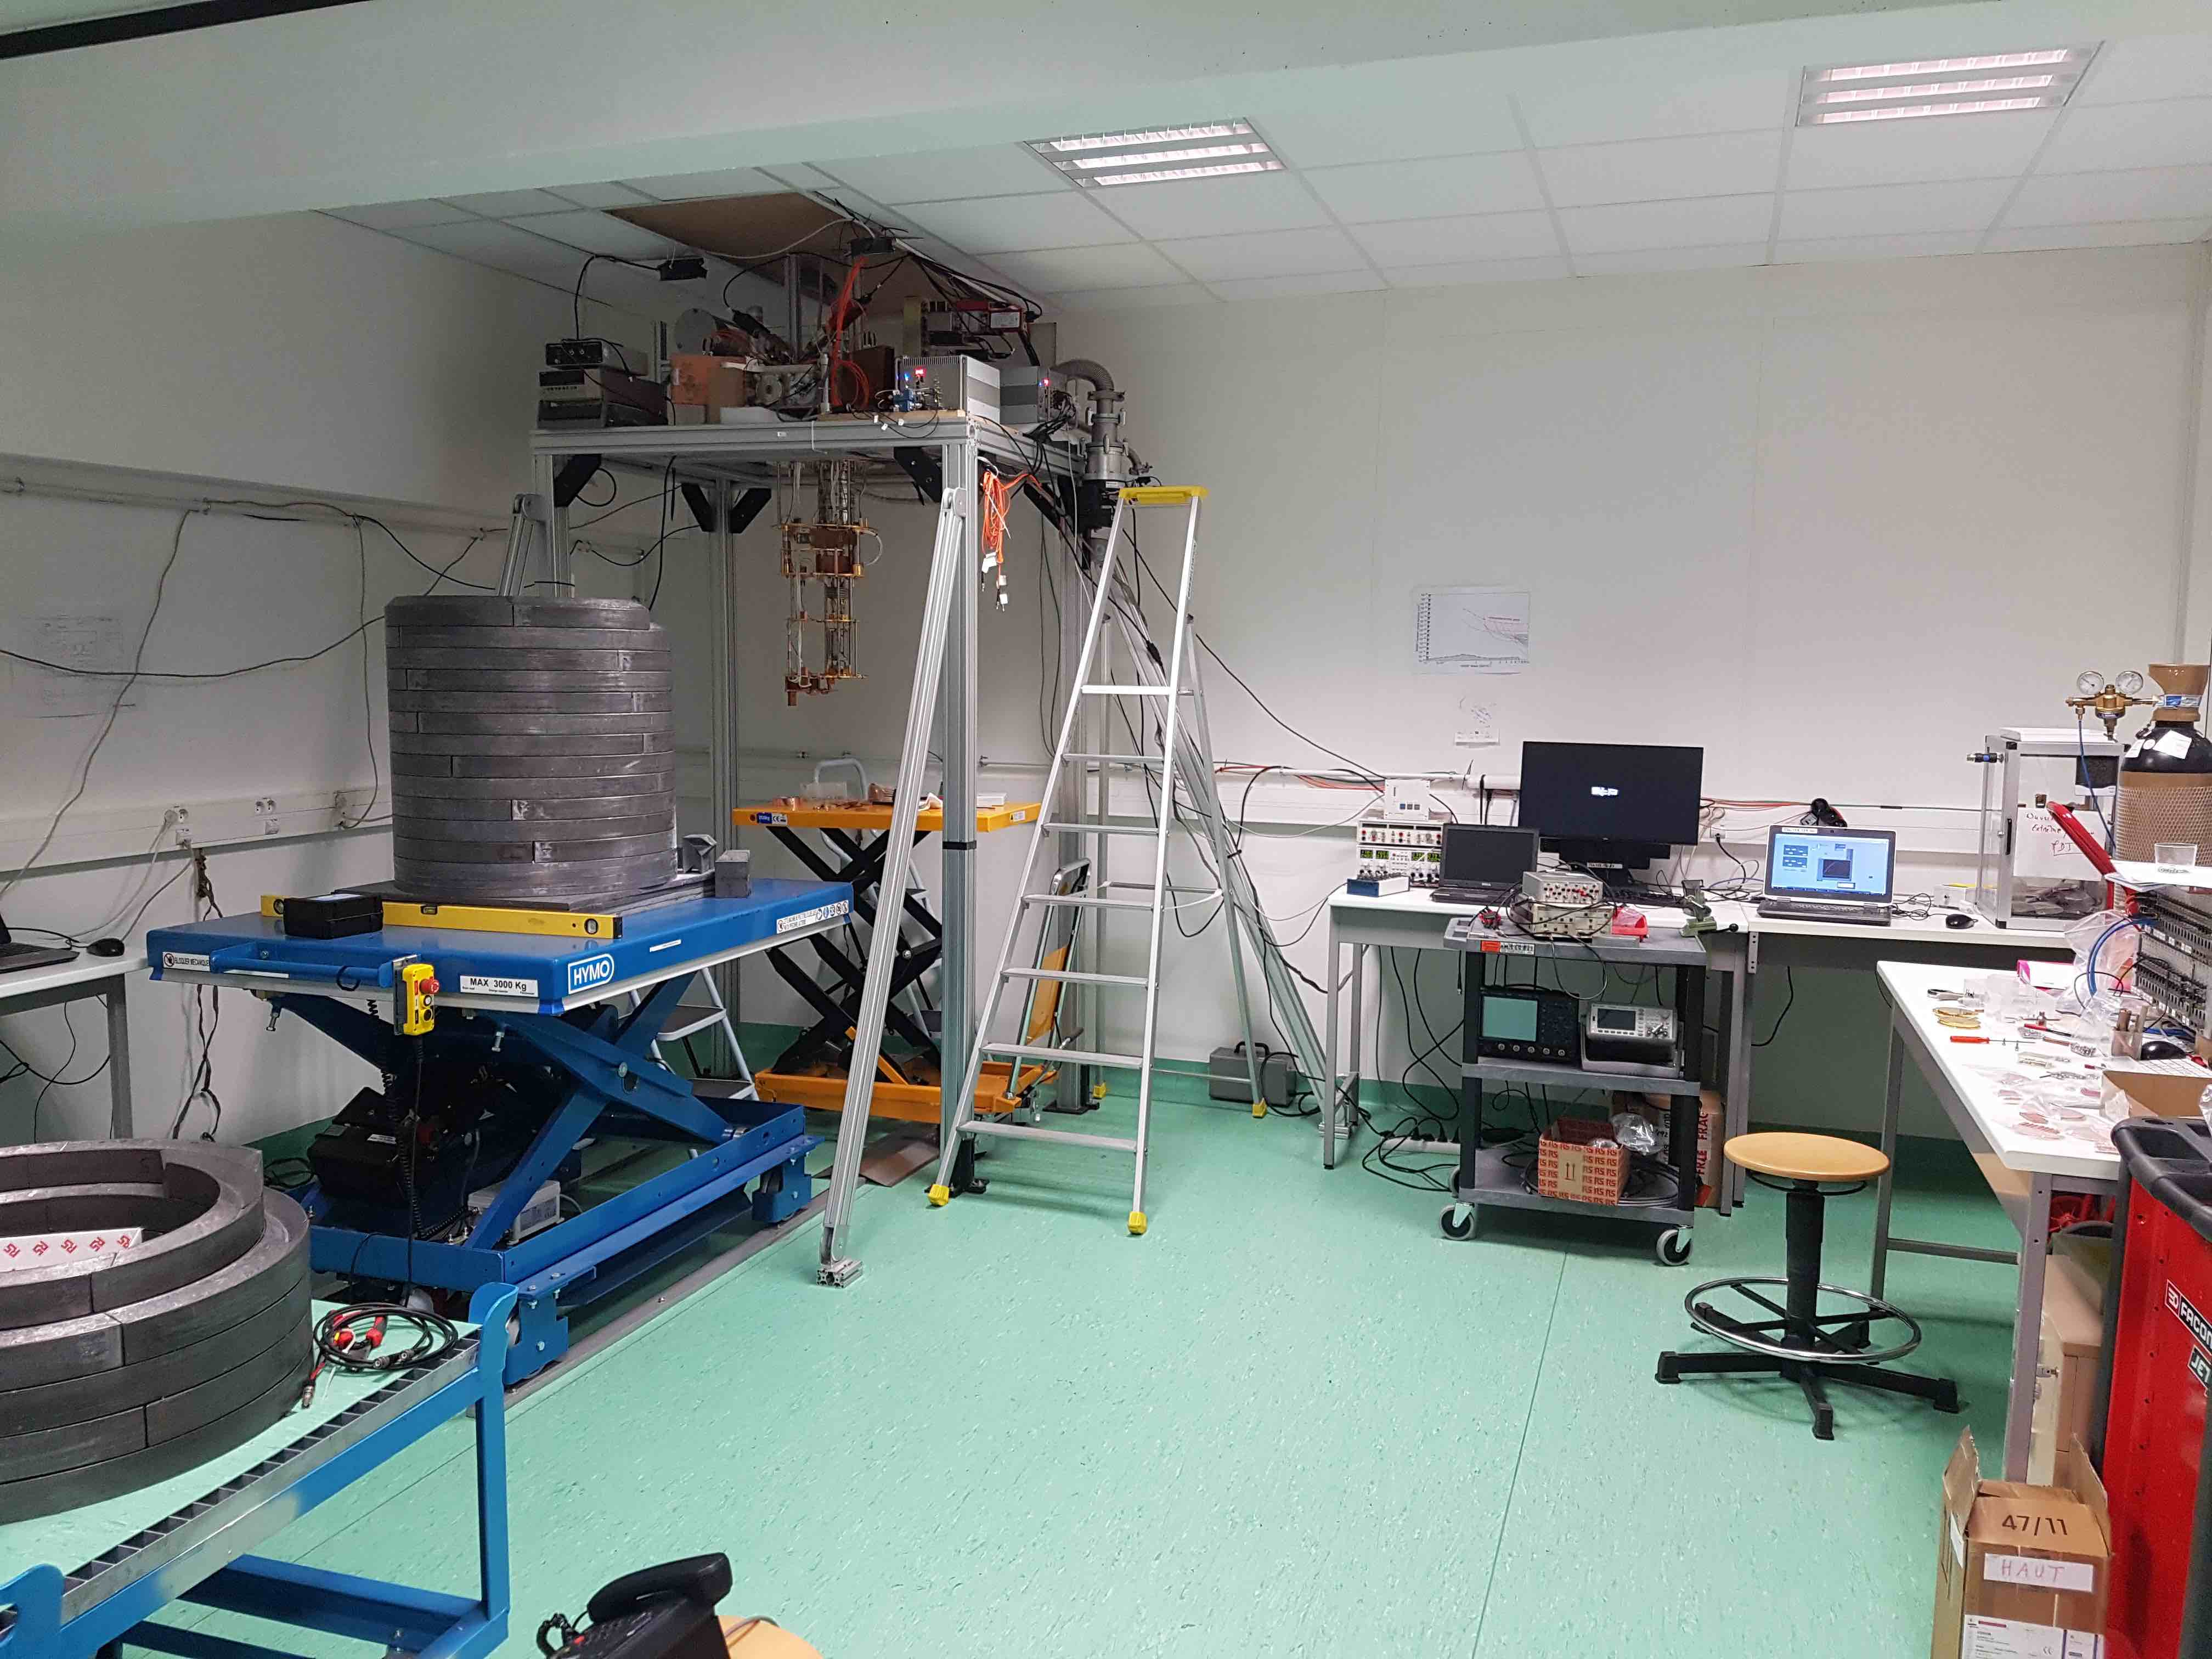
\includegraphics[width=\textwidth,angle=0]{Figures/Experiment/ip2i_cryogenic_facility.jpg}
\caption{Photo of the cryogenic lab, where the dry dilution cryostat (opened) and its lead shield are clearly visible. 
%On the left side are the computers controlling the cryostat, and 
On the right side are the computers and outside electronics in charge of the detector readout and polarization.}
\label{fig:cryolab}
\end{center}
\end{figure}

\subsection{Presentation of the IP2I R\&D Dry Cryostat}

% Cryostat intro
The cryostat is a Hexadry-200 commercially available from Cryoconcept, which has been upgraded to reduce the vibration levels at the mixing chamber.
The cryostat assures a cryogenic temperature with low fluctuations and a temperature setpoint of about \SI{10}{\milli\kelvin} for the bolometer operation. It provides a steady cooling power over several weeks for standard R\&D runs which can be extended to several months for physic runs.

% Cryostat structure
The structure of the cryostat is illustrated with annotated photo and scheme displayed in the figure \ref{fig:cryo-photo}. This cryostat is built with several cooling stages at different temperatures which allow the transition from the exterior ambient temperature $\sim \SI{300}{\kelvin}$ to the lowest cryogenic temperature $\sim \SI{10}{\milli\kelvin}$ on the mixing chamber. During operation, the cryostat is maintained hermetically shut with the Outer Volume Casing (OVC) mounted on the feedtrough of the cryostat. The whole inner volume is immersed in a medium vacuum, the air is pumped out to reach a pressure less than \SI{e-5}{\milli\bar}). As such, there is no gas to conduct heat between the different stages. The thermal conduction between stages can only occur though the metal structure of the cryostat, the cooling circuit and the thermal radiation. Each stage is surrounded by gold-plated copper casings to block the infrared radiation from various stages.

\begin{figure}
\centering
\begin{minipage}{0.48\textwidth}
	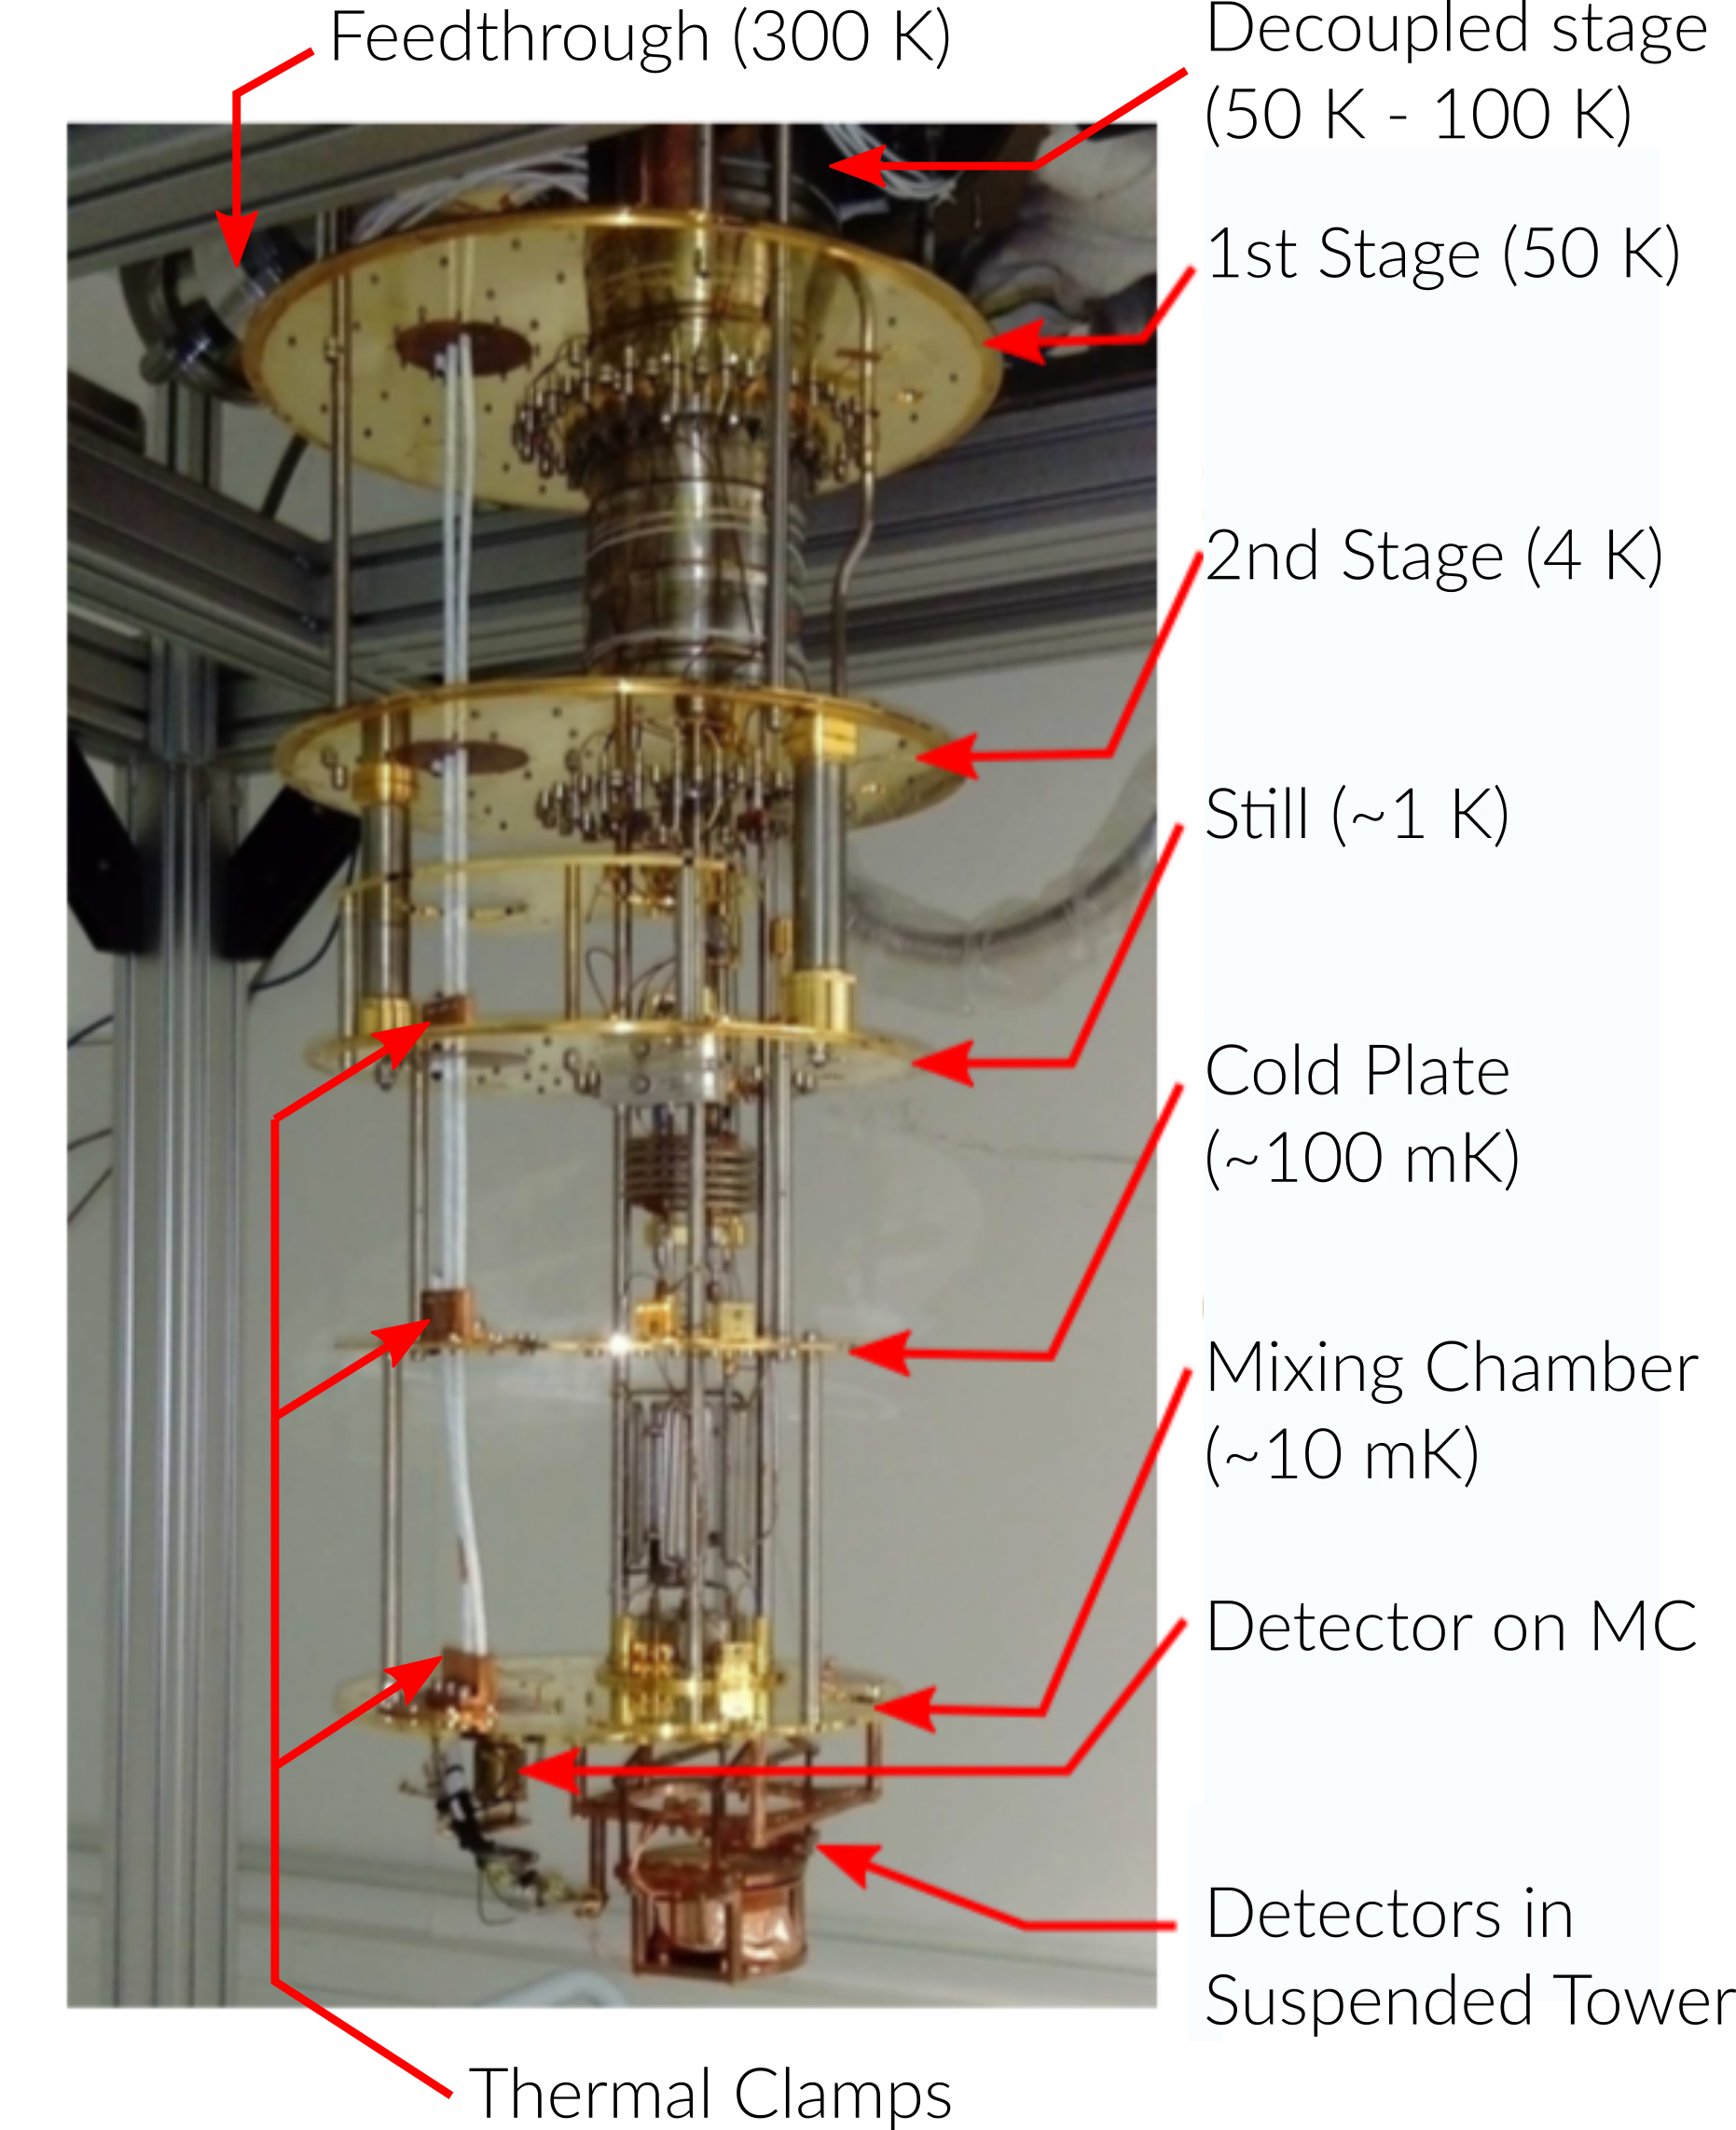
\includegraphics[width=\textwidth]{Figures/Experiment/cryo_photo.png}
\end{minipage}
\hfill
\begin{minipage}{0.48\textwidth}
	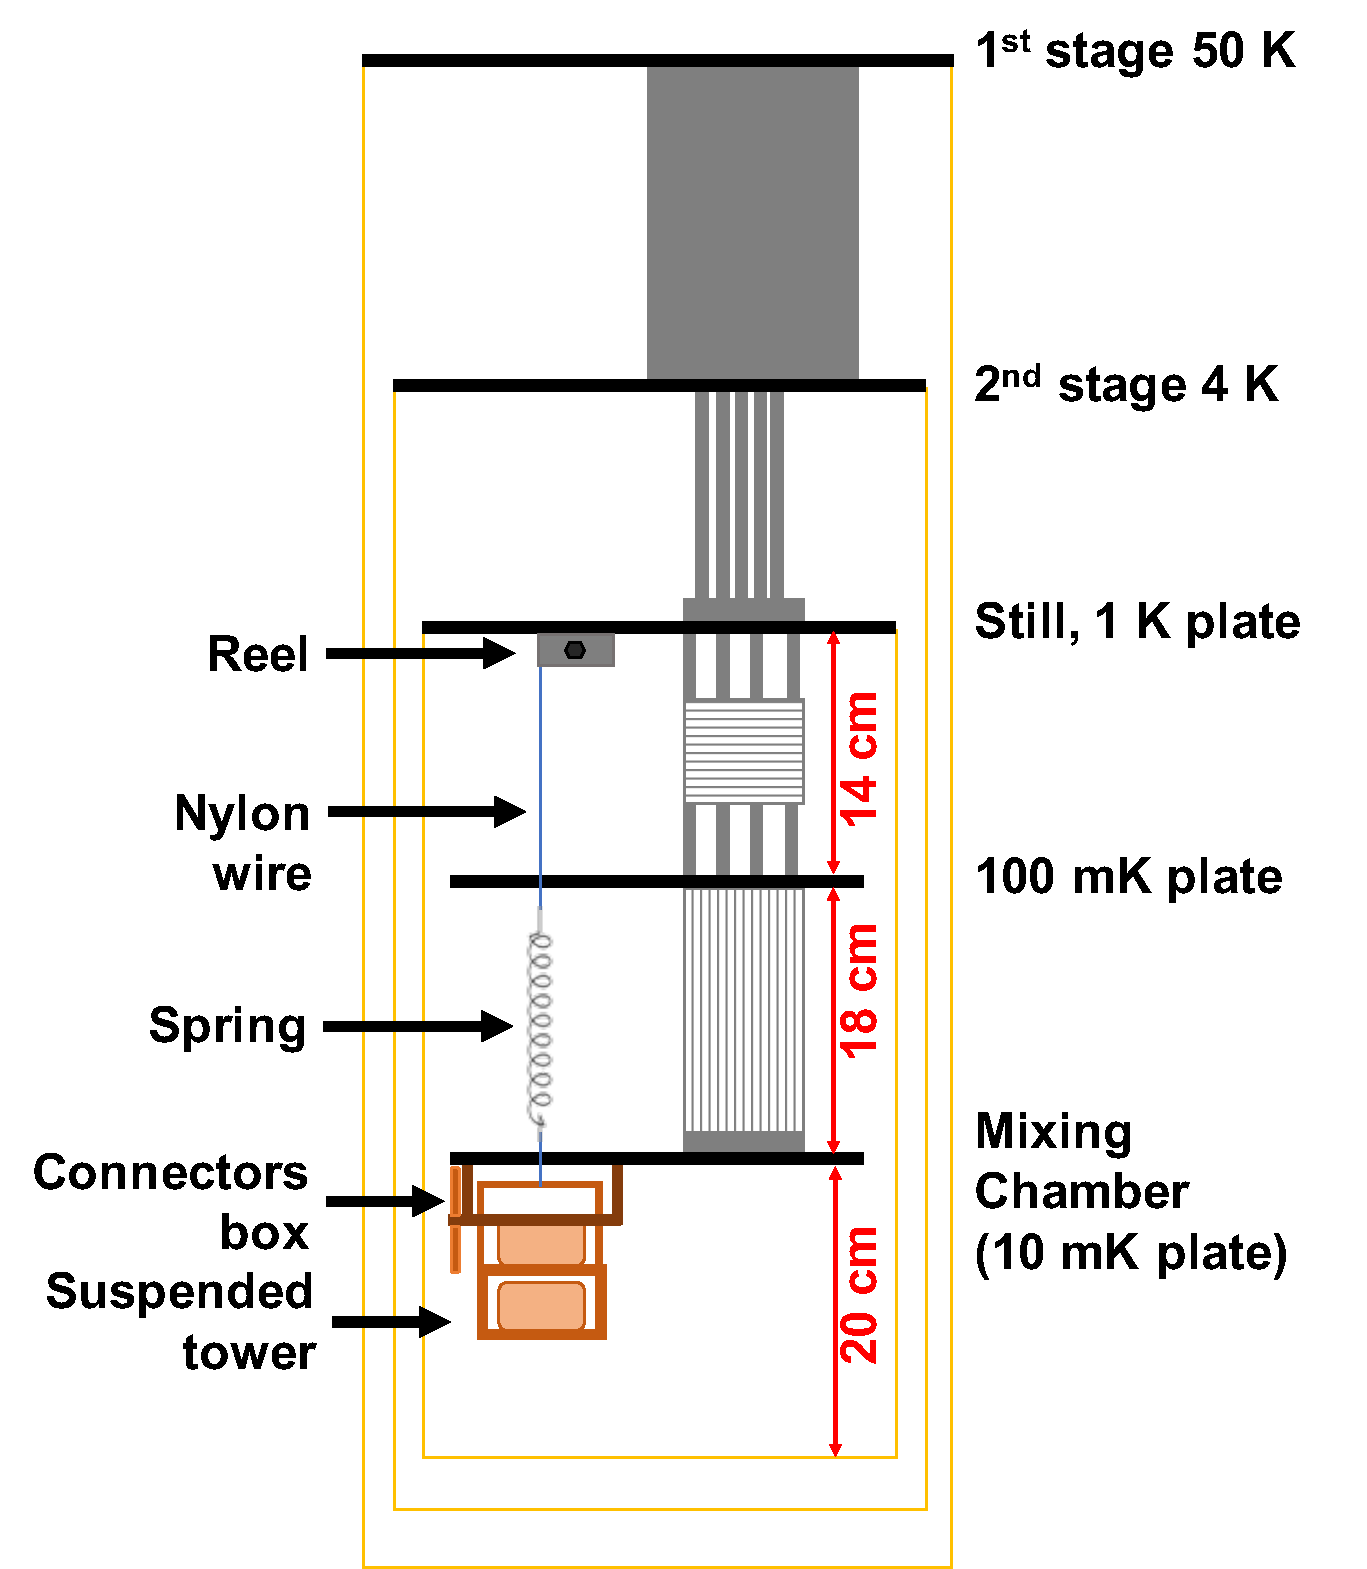
\includegraphics[width=\textwidth]{Figures/Experiment/cryo_sketch.pdf}
\end{minipage}
\caption{On the left, annotated photo of the open cryostat. On the right, annotated scheme of the cryostat. The copper screens blocking the infrared radiations are represented as the orange rectangles separating each cooling stage. Figures taken from \cite{Maisonobe:2018tbq}.}
\label{fig:cryo-photo} 
\end{figure}

% Dry cryostat
The IP2I cryostat is a Dry Dilution Refrigerators (DDR). It runs solely on electric power as opposed to the Wet Dilution Refrigerators (WDR) of the \Edelweiss{} experiment which consumes liquid helium to cool down. Dry cryostats are particularly adapted to R\&D work as the operating cost is low and it is possible to descend very quickly to cryogenic temperatures (24 hours to reach \SI{4}{\kelvin}, compared to one week for the \Edelweiss cryostat at the LSM\footnote{Laboratoire Souterrain de Modane, France}). They provide a similar low temperature environment as the one obtained with WDR at the cost of increased vibration levels. The IP2I cryostat was equipped with vibration mitigation solutions described in the next section \ref{sec:suspended-tower}.

% Cooling circuit
The IP2I dry cryostat has one closed cooling circuit using as cooling fluid a mixture of \SI{75}{\percent} \ce{^4He} and \SI{25}{\percent} \ce{^3He}. This cooling circuit is separated in two cycles: the "Pulse Tube" cycle and the dilution cycle. 
% Pulse tube cycle
The pulse tube cycle is in charge of cooling the first stage and second stage to reach the temperatures \SI{50}{\kelvin} and \SI{4}{\kelvin} respectively. The "Pulse Tube" applies Stirling cycles between 9 and 18 bars at a frequency of \SI{1.6}{\Hz}, which allows the \ce{{}^4He} fluid to reach a temperature of \SI{4}{\kelvin}.
% The dilution cycle
The dilution cycle extends the cooling circuit to the three other stages and cools them to their operating temperatures: the still at $\sim\SI{1}{\kelvin}$, the cold plate at $\sim \SI{100}{\milli\kelvin}$ and the mixing chamber (MC) at $\sim \SI{10}{\milli\kelvin}$. In this cycle, the helium mixture is cooled by passing through fine capillaries located on the first and second stages, benefiting from the cooling of the pulse tube cycle. As the cooling fluid reaches \SI{4}{\kelvin}, it condensates in its liquid phase. A succession of Joule-Thompson expansions and heat exchangers allows the mixture to reach a temperature of \SI{800}{\milli\kelvin} at the still. It is near this temperature that a phase separation occurs within the mixture: the first phase is concentrated in \ce{{}^3He} and floats on the surface of the second phase diluted in \ce{{}^3He} and rich in \ce{{}^4He}. This phenomenon can be explained by the Fermi-Dirac statistic followed by the \ce{{}^3He} atoms: they cannot simultaneously occupy the same energy state and the same position. Thus, for a sufficiently low temperature, the phase separation becomes energetically favorable. This phase separation takes place within the mixing chamber. The phase with low \ce{{}^3He} is then pumped out. The thermodynamic equilibrium of the two phases is broken and there is a transfer of \ce{{}^3He} from the concentrated phase to the diluted phase in \ce{{}^3He}. This process is endothermic, which decreases the temperature of the mixture and thus of the mixing chamber. The pumped helium \ce{{}^3He} is then re-injected into the dilution circuit. To this end, the dilution cycle allows a minimum temperature of \SI{9}{\milli\kelvin} to be reached on the mixing chamber for this cryostat. The detector load is thermally linked to the mixing chamber in order to reach the lowest temperatures and the best performances.

% Thermal regulation
Once the cryostat is cooled down, it continues to operate at full power until the end of the run. The power of the cooling circuit is in constant equilibrium with the thermal heat coming from the exterior of the cryostat or from the operation of the detectors. Consequently, in this state, the exact temperature of the mixing chamber would fluctuate near its minimal equilibrium value. 
As a mean to operate the cryogenic detectors with constant performances and at a chosen temperature, the latter is regulated at higher temperatures usually superior to \SI{14}{\milli\kelvin}. The regulation is assured by the Joule effect of a heating resistor. Its heat power is set by a Proportional-Integrate-Derivative controller (PID controller) reading the temperature with a \ce{RuO_2} thermistance close to the detectors in the suspended tower.


\subsection{Standard Operation of the Detectors}

% detector load and electronics
We want to operate the bolometers at the coldest temperature possible. We may want to attach the detectors directly on the mixing chamber stage as seen on left photo of figure \ref{fig:cryo-photo}. However, the "dry" cryostat creates a lot of mechanical vibration especially due to the pulse tube operation. These vibrations propagate to the detectors, causing thermal noise (parasitic phonons), electric noise (triboelectricity) as well as heat power on the mixing chamber which prevents a good cooldown \cite{Olivieri:2017lqz}.
To tackle this issue, the cryostat is mechanically decoupled from the ceiling/pulse tube with a bellow (external decoupling). This external decoupling was done in partnership with Cryoconcept by mechanically decoupling the cold head of the pulse tube cryocooler from the dilution unit. The vibrations at the detector level were further mitigated by placing the bolometers inside a suspended tower (internal decoupling) developed by the MANOIR group \cite{Maisonobe:2018tbq}.
The suspended tower is a copper chassis solely linked to the cryostat by a spring providing mechanical support and mechanical decoupling. This device makes it possible to avoid a significant low-frequency noise on the heat measurement while ensuring thermal conduction to the cryostat thanks to thin copper braids. This suspended tower is described in the paragraph \ref{sec:suspended-tower}.

The detectors are cabled to the acquisition computer on the outside of the cryostat through the cold and warm electronics. The cold electronics transports the voltage signal of the detectors located near the mixing chamber to a first Bi-FET preamplifier stage at \SI{100}{\kelvin} and a second stage amplifier at \SI{300}{\kelvin} \cite{Armengaud:2017rzu}.
The white cables of this cold electronic are visible on the left photo of figure \ref{fig:cryo-photo}. The cabling comes from the top of the cryostat and goes down to the dilution and is thermalized at each stage thanks to thermal clamps. As such, there is only minimal heat transfer from the hotter stages  on the mixing chamber due to the electronics.
Once the signal is amplified, it is transported to the acquisition computer with optical fiber. The detector signals are recorded as continuous time series called data streams. These data streams are then processed with a dedicated pipeline based on the NEPAL software developed by the MANOIR group in order to ensure high quality data processing. The stream processing and analysis is described in Chapter \ref{ChapterElectrodesExperimental}. Once the processing is done at the CC-IN2P3, monitoring plots are transferred automatically to a monitoring website allowing us to follow the performance and behavior of the detectors as a function of time.

%%% Bonus
%% IP2I Cryostat for Ricochet 
%By early 2021, our cryogenic lab will be hosting the \Ricochet{} cryostat for a little over one year in order to be fully commissioned prior to its deployment at ILL. The commissioning phase includes: validation of the cabling (noise and thermal performance), the cold front-end electronics, the cool down of the inner shielding layers (lead and polyethylene), the demonstration of the CryoCube detector array performance (threshold, particle identification capability and livetime), and the DAQ and monitoring pipelines.


\section{Vibration mitigation and cryogenic suspension}
\label{sec:suspended-tower}
\label{par:suspended-tower}

% Motivation
The cool-down process of the two first stages within DDR is ensured by the technology of pulse-tube cryocoolers. However, the mechanical vibrations they induce can drastically affect the performance of cryogenic detectors. This effect has been reported by several cryogenic experiments using such bolometers ( see \cite{Maisonobe:2018tbq} and references there in).
%\cite{Caparrelli:2006zkj,Haan:2013iwa,Olivieri:2017lqz}. 

% external mitigation
The IP2I cryostat was upgraded with an external vibration mitigation solution. Its first two stages (50K and 4K) are thermally coupled to the highly vibrating pulse-tube cold head thanks to low-pressure gas exchangers (Hexagas$^{\rm TM}$), hence avoiding any mechanical contact and vibration propagation to the dilution unit. In 2016, one year after its delivery to IP2I, the cold head has been mechanically anchored to the ceiling hence providing two independent and maximally decoupled frames. As shown in the figure \ref{fig:cryolab}, the metallic framework surrounding the cryostat supports and anchors the dilution unit to the ground, while the cold-head is fixed to the ceiling of the laboratory (hidden by a wooden panel on the photo).

% results
This upgrade led to the reduction of the vibration levels by about two orders of magnitude between \SI{0.5}{\Hz} and \SI{20}{\Hz} hence achieving world-leading vibration levels in a dry cryostat of few-\si{\micro g \per \sqrthz} below \SI{20}{\Hz} \cite{Olivieri:2017lqz}.
At the time, the impact on our detectors has been tremendous. Indeed, before the decoupling, due to the high vibration levels, the detectors were not able to operate due to the significant vibration-induced  frictional heat power dissipation. 

% Motivation internal
% External Mitigation results 
With the improvement of our detector sensitivity and resolution, we found that the cold-head decoupling was not enough to ensure optimal operation of the new generation of detectors. Indeed, it was found that the large radial stiffness of the edge-welded below connecting the cold-head to the dilution unit still allowed for some vibration propagation down to the detectors. A second vibration mitigation system at the mixing chamber level, where the detectors are installed, had to be implemented.


\subsection{Internal Mitigation Solution: the Suspended Tower}

%% Internal mitigation
%This internal vibration mitigation is the suspended tower presented in the annotated photo \ref{fig:suspended-tower}. This device consists in a 25 cm long elastic pendulum, attached to the \SI{1}{\kelvin} stage by a Kevlar string and a stainless steel spring with an elastic constant of \SI{240}{\newton\per\meter}, holding the detector tower situated below the mixing chamber at \SI{10}{\milli\kelvin}. The detector tower is thermally anchored to an intermediate safety structure via supple copper braids. This safety structure also hosts the connectors for the detector readout.

% suspended tower theory
This internal vibration mitigation solution is the suspended tower which can be considered as a simple elastic pendulum.
The 3-D dynamical description of the elastic-pendulum can be divided into two pseudo-independent equations in the approximation of small perturbations. The natural frequency for vertical modes is then given by:
\begin{equation}
\label{eq:Freq-Vertical}
f_{0,\textrm{vertical}}=\frac{1}{2\pi}\cdot\sqrt{\frac{k}{M}} = \frac{1}{2\pi}\cdot\sqrt{\frac{g}{(l_{\textrm{eq}}-l_{0})}}
\end{equation}
where $M$ corresponds to the total mass of the suspended tower, $k$, $l_0$, and $l_{\rm eq}$ are the elastic constant, the rest length, and the length at equilibrium of the spring, respectively. The vertical resonance frequency can either be expressed in terms of $k$ and $M$ simultaneously or by the spring elongation alone $|l_{\textrm{eq}}-l_{0}|$. The natural frequency for radial oscillations of the pendulum, which are related to its total length  $l_{\rm tot}$, is given by:
\begin{equation}
f_{0,\textrm{ radial}}=\frac{1}{2\pi}\cdot\sqrt{\frac{g}{l_{\rm tot}}}\label{eq:Freq-Radial}.
\end{equation}
From these approximations, we can estimate the theoretical resonance frequencies of the elastic pendulum depending on the spring constant, the pendulum length and the total mass of the detector assembly. Interestingly, one can notice that as $l_{\textrm{tot}} \geq (l_{\textrm{eq}}-l_{0})$, the natural frequency in the radial direction is necessarily lower than in the vertical direction: $f_{0,\textrm{ radial}}<f_{0,\textrm{vertical}}$. 

Thanks to the use of a single spring holding system, we avoid any transverse momentum related natural frequencies which could populate the vibration spectrum at high frequencies. Therefore, the system is expected to have a transfer function response under the form of a 2\textsuperscript{nd} order low-pass filter with a single resonance frequency in both directions $i=\left\{ \textrm{vertical, radial}\right\}$:
\begin{equation}
H(\omega_{i})=\frac{\omega_{0,i}^{2}}{\omega_{0,i}^{2}-\omega_{i}^{2}}\label{eq:Transfer-function},
\end{equation}
where $\omega_{0,i}$ is the natural pulsation of the suspended tower, with $\omega_{0,i}=2\pi\cdot f_{0,i}$. 
The natural frequencies of the suspended tower in both vertical and radial directions have been tuned to be as low as possible in order to attenuate all vibrations above \SI{1.4}{\Hz}, corresponding to the frequency of the pulse-tube cryocooler. According to equation \ref{eq:Freq-Vertical}, we obtain a vertical resonance frequency $f_{0,\textrm{vertical}} \leq \SI{1}{\Hz}$ for a spring elongation of at least $(l_{\textrm{eq}}-l_{0})\geq \SI{25}{\cm}$. The same condition applied to the radial frequency, $f_{0,\textrm{radial}} \leq \SI{1}{\Hz}$ results in a total pendulum length of at least  $l_{tot}\geq \SI{25}{\cm}$ using equation \ref{eq:Freq-Radial}.

The challenge then comes from accommodating with the constraints imposed by the cryostat geometry. As the distance between the mixing chamber plate and the inner thermal screen is only of about \SI{18}{\cm}, the pendulum had to be attached to the still plate and not directly to the mixing chamber.
The scheme of the figure \ref{fig:cryo-photo} and the photo \ref{fig:suspended-tower} illustrate the holding strategy of the suspended tower in the cryostat. 
A Kevlar wire is fixed below the still plate at \SI{1}{\kelvin} and running without contact through the cold plate at \SI{100}{\milli\kelvin}. 
A stainless steel spring with an elastic constant of $k=\SI{240}{\newton\per\meter}$ is attached to the wire between the cold plate and the MC at \SI{10}{\milli\kelvin}. The elastic constant $k$ has to be carefully chosen, taking into account the total mass of the detector assembly $M$, as its elongation is constrained by the $\sim \SI{18}{\cm}$ distance between the \SI{100}{\milli\kelvin} stage and the MC. 
Finally, the suspended tower is connected to the spring via a thick ($\sim \SI{2}{\mm}$ in diameter) \SI{5}{\cm} long copper wire through the MC plate. This copper wire ensures the thermalization of the stainless steel spring, so that it does not emit infrared radiation damaging the detector performance.
With this approach, the total pendulum length from the still plate to the center of mass of the detector assembly is $l_{\textrm{tot}} = \SI{25}{\cm}$.


\begin{figure}
\centering
\captionsetup{justification=centering}
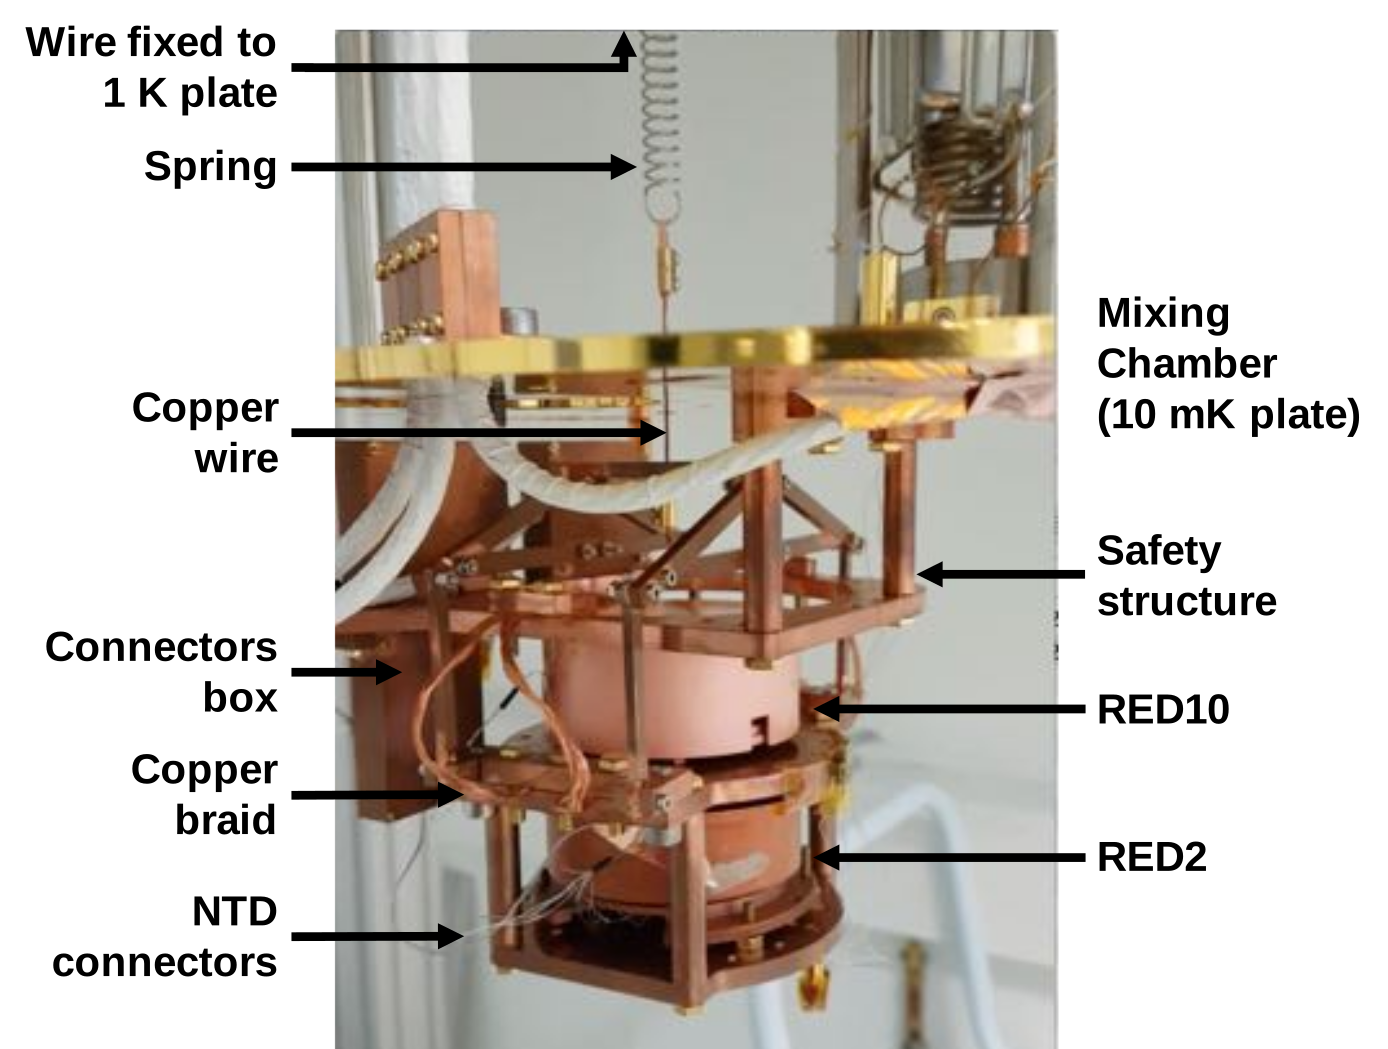
\includegraphics[height=9cm]{graphics/damocles.png}
\caption{Photo of the suspended tower containing the two $\SI{200}{\g}$ bolometers RED10 and RED2. This device mechanically decouples the detector load from the mixing chamber while assuring its thermalization. Figure taken from \cite{Maisonobe:2018tbq}.}
\label{fig:suspended-tower} 
\end{figure}

The detector tower is shown in the figure \ref{fig:suspended-tower} holding the two detectors RED2 and RED10. This module has a total height of \SI{13}{\cm} and can hold two cryogenic detectors based on \SI{200}{\g} germanium crystal or lighter. During the installation, before attaching the spring, the tower is firmly held by a copper frame screwed under the MC plate. This structure remains as a safety structure during cool-down and operation in case the wire should break. Connector boxes are placed close to the detector on the external side of the safety structure. They are used to connect the sensors of the detectors to the readout electronics at the warmer stages. Both the suspended tower and the safety structure are made of radiopure \ce{CuC_2} copper. During operation, the suspended tower is floating and its thermalization is realized by four \SI{10}{\cm} long ultra-supple flat copper braids linking the safety structure and the tower.


\subsection{Characterization of the Vibration Levels}

This subsection quickly presents the impact of the suspended tower on the vibration level and the noise of the heat channel of the bolometer RED10. All the results are published in the paper \cite{Maisonobe:2018tbq} in which the suspended tower was demonstrated to attenuate the transmission of both vertical and radial vibrations, with a particular emphasis on the radial modes as these are less efficiently damped from our pulse-tube cold head decoupling. 

The vibration level is characterized by measuring the movement of the detectors \cite{Olivieri:2017lqz}.
The set-up is composed of a high sensitivity seismic accelerometer from \emph{PCB Piezotronics}. We used the high sensitivity accelerometer \emph{PCB-393B05} which has a gain of \SI{10}{\volt\per g} and an intrinsic noise limit of $\textrm{[0.5-0.07]}\,\textrm{g}/\sqrt{\textrm{Hz}}$ within $\textrm{[1-1000]}\,\si{\Hz}$ frequency range.

The accelerometer is fixed on a U-shaped workpiece allowing to measure the vibrations along either the radial or the vertical direction.  The accelerometer can be fixed below the MC stage of the cryostat, or below the bottom stage of the suspended tower in order to compare their respective vibration level. 
The elastic constant $k$ and Young's modulus $E$ values of the stainless steel and copper, composing the majority of the rigid strucutre of the cryostat, have small variations between ambient and cryogenic temperatures. As such, all vibration measurements are performed at room temperature \cite{Emodulus}.
The output signal of the accelerometer is sampled at \SI{10}{\kilo\Hz}, well beyond the signal bandwidth of the accelerometer of \SI{1}{\kilo\Hz}. The vibration levels is obtained as LPSD expressed in \si{g \per \sqrthz} from a Fast Fourier Transform (FFT) analysis using Hanning windowing over \SI{5}{\s} time windows.
Figure~\ref{fig:vibration-levels} displays the vibration levels on the MC plate and in the suspended tower comparing the measurements with the pulse-tube (PT) cryocooler switched on (PT ON), emulating the normal cryostat operation, or off (PT OFF). The intrinsic noise limit of the accelerometer is plotted as dashed lines as reference.

\begin{figure}
\centering 
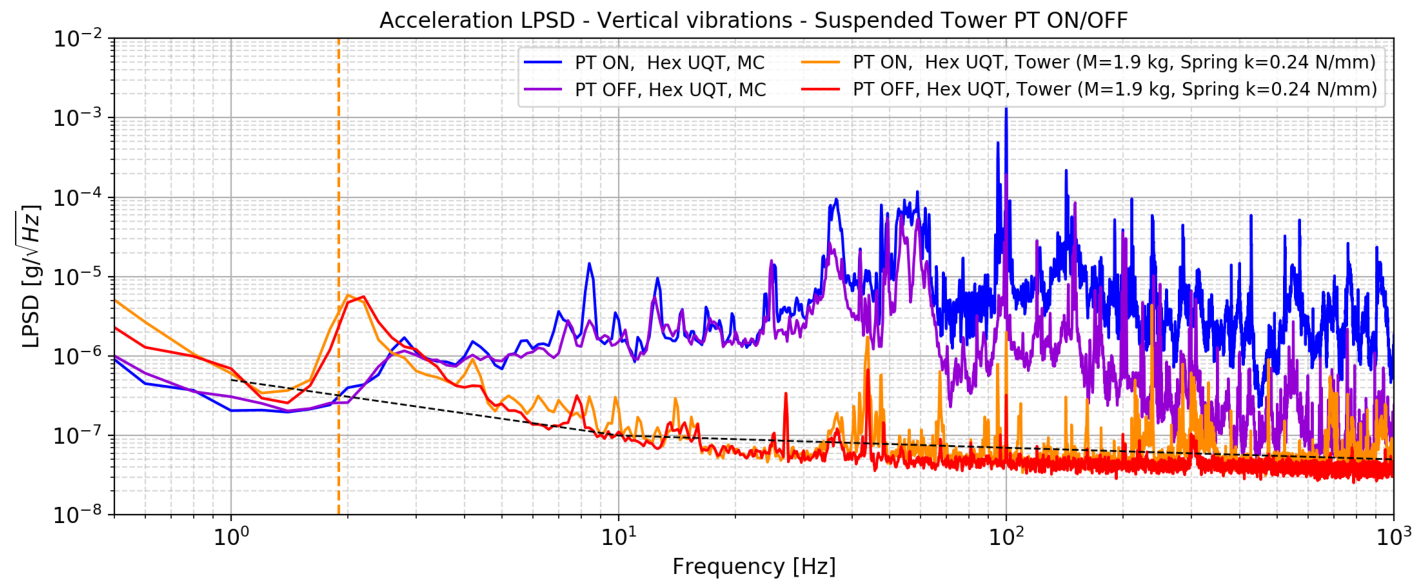
\includegraphics[width=\textwidth]{Figures/Experiment/vibration_vertical.pdf}
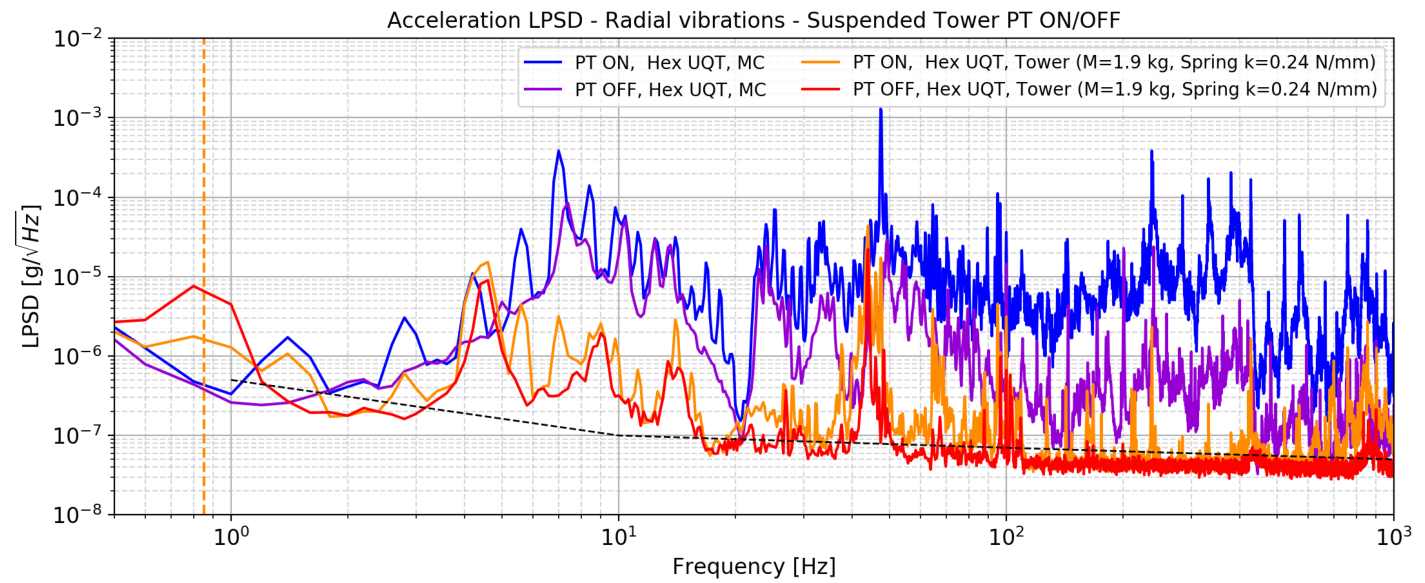
\includegraphics[width=\textwidth]{Figures/Experiment/vibration_radial.pdf}
\caption{Comparison of the vertical (top subplot) and radial (bottom subplot) vibration levels of the MC plate and the suspended tower in both PT ON and OFF configurations. The dashed black line is the accelerometer sensitivity, and the orange vertical dashed lines represent the position of the natural frequencies of the suspended tower derived from equations \ref{eq:Freq-Vertical} and \ref{eq:Freq-Radial}. Figures taken from \cite{Maisonobe:2018tbq}.}
\label{fig:vibration-levels}
\end{figure}

The main differences observed between these two PT configurations are coming from few pick-up lines which are mostly at high frequencies and arise from the acoustic noise generated by the operation of the pulse-tube cooling cycle.
At low frequencies ($<\SI{40}{\Hz}$), in the detector bandwidth, the impact of turning the PT ON is very small on the suspended tower, merely being expressed as resonance peaks of low amplitudes.
As a matter of fact, by comparing the vibration level of the MC plate in the PT OFF case (purple solid line) to the level of the suspended tower in the PT ON case (orange solid line), one can further conclude that the suspended tower is not only efficient at reducing the PT-induced noises but also most of the whole setup-related vibrations from the building, the cryostat holding structure, and so on.
This demonstrates that vibration-wise, our detectors are largely insensitive to their surrounding environment, suggesting that they should run in optimal conditions inside the IP2I cryostat.

% Noise level for RED10
This optimal operation condition can be checked by comparing the noise level affecting the signal measurement of a detector either installed on the mixing chamber plate or in the suspended tower. In this paragraph, this comparison is made with the \SI{200}{\g} detector RED10 whose heat channel is later characterized in the chapter \ref{ChapterEthem}. With a heat sensitivity of about \SI{100}{\nano\volt\per\kilo\eV} at around \SI{18}{\milli\kelvin}, RED10 is sensitive to perturbative displacements and vibrations. 

The noise levels are presented as LPSD expressed in \si{\volt\per\sqrthz}. These LPSD were measured as presented in section \ref{par:ethem-noise} dedicated to the characterization of the electronics noise affecting the heat channel of the bolometers.

Figure \ref{fig:red10-vibration} shows the LPSDs obtained for RED10 on the MC plate as dashed lines, and on the suspended tower as solid lines. The \SI{1}{\volt} normalized heat signal template power spectrum and the theoretical noise calculations based on the full electro-thermal modeling of the detectors (see Sec.\ref{sec:ethem-noise}) are also plotted as a reference. Measurements of the LPSDs were made with and without polarizing the heat sensor (called NTD and described in section \ref{sec:detector-principle}) of RED10 in order to estimate the effect of the vibrations on the cabling, such as microphonics. Note that the discussion will mostly focus on the frequency range of interest, from \SI{1}{\Hz} to \SI{40}{\Hz}, as it corresponds to the detector signal bandwidth.

\begin{figure}
\centering 
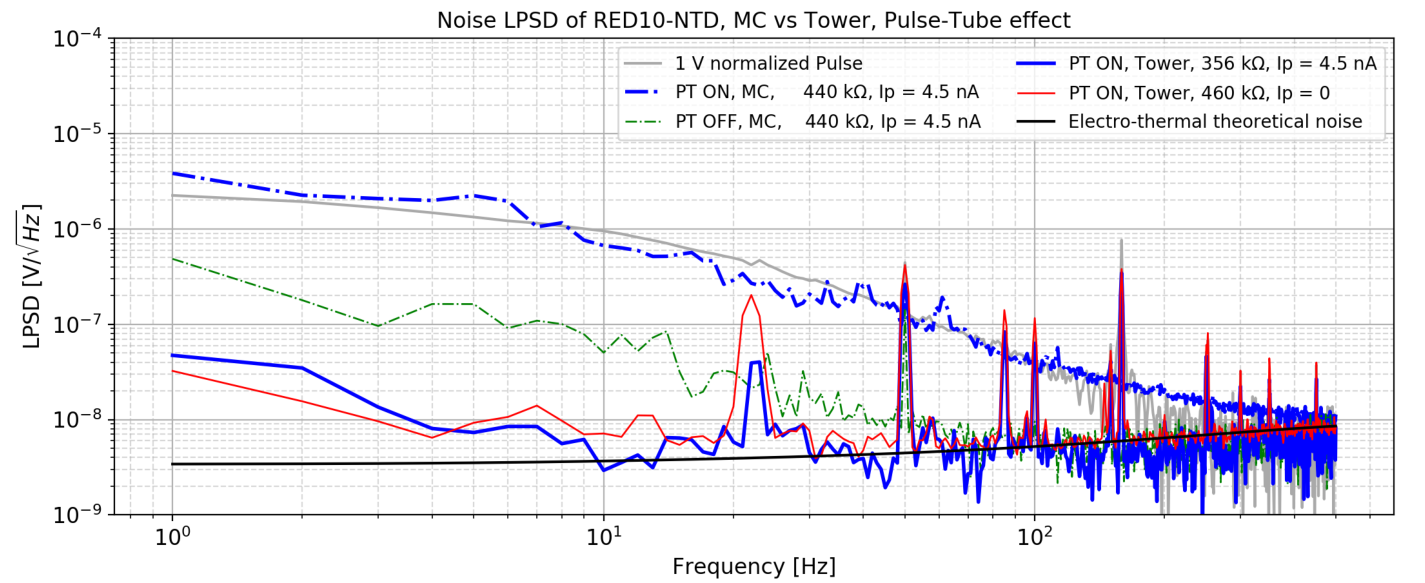
\includegraphics[width=\textwidth]{Figures/Experiment/red10_lspd_vibration.pdf}
\caption{Noise power spectra density for the NTD of RED10 mounted on the MC plate (dashed lines) and on the suspended tower (solid lines). Measurements were performed at optimal NTD polarization currents with PT ON and PT OFF at \SI{16}{\milli\kelvin}. The black solid line refers to the expected noise level derived from the electro-thermal model described in section \ref{sec:ethem-noise}, while the grey solid line shows the unit normalized pulse template illustrating the signal bandwidth. Figures taken from \cite{Maisonobe:2018tbq}.}
\label{fig:red10-vibration}
\end{figure}


From comparing the various voltage PSD presented in Figure \ref{fig:red10-vibration}, we can extract a few major conclusions regarding the effectiveness of the suspended tower at mitigating the vibration-induced noise on bolometers. 

The first obvious comparison is between the cases where the detectors are optimally polarized (blue curves) and either on the mixing chamber (dashed lines) or on the suspended tower (solid lines). The LPSD at the lowest frequencies is reduced by almost two orders of magnitude. 
Furthermore, we observe that the noise levels obtained PT ON and with the NTD optimally polarized (blue solid lines) are almost identical to the case where the NTDs are not polarized and the pulse-tube OFF (red dashed lines), suggesting that we are limited by both the electronics and the intrinsic thermal noise from the detector, and not by the vibrations when the detectors are mounted on the tower.
 This is confirmed by the fact that the resulting noise levels are very close to the theoretical expectations obtained with the electro-thermal model illustrated by the black solid lines.

Interestingly, we do not see on the NTD a \SI{1.8}{\Hz} pick-up noise as was potentially suggested from the vertical acceleration measurements shown as the red (PT OFF) and orange (PT ON) solid lines from Figure~\ref{fig:vibration-levels}. This  suggests that such frequency vibrations within the detector bandwidth do not limit the detector performance.

Finally, one can derive from Figure~\ref{fig:red10-vibration} that the noise PSD obtained with the NTDs optimally polarized on the suspended tower with PT ON (blue solid lines) are below the ones obtained with the detectors running on the mixing chamber with the PT OFF (green dashed lines). This observation confirms what was suggested from the vibration measurements shown in figure \ref{fig:red10-vibration}:  the suspended tower damps very efficiently the vibration-induced noise from the pulse-tube cryocooler, but makes the detectors insensitive to any residual vibrations from the surrounding environment of the experiment

The improvement on RED10 performance can be appreciated by computing its energy resolution. It was found that the heat resolution of RED10 improved from \SI{14}{\kilo\eV}, when installed on the mixing chamber, to \SI{400}{\eV}  when installed in the suspended tower. This impressive gain of almost two orders of magnitude on the energy resolution can be explained by the detector RED10 being especially susceptible to vibrations. This detector would have been discarded due to poor performances without this internal mitigation solution.

%\footnote{Note that since this work, tremendous progress have been made on the low-noise cold cabling, the processing tools, and the low-energy calibration, such that RED10 actually achieved 50~eV (RMS) heat energy resolution later on, see Sec.~\ref{sec:randd-heatperformance}}.

Following the publication of this work \cite{Maisonobe:2018tbq}, similar improvement factors were found, between a factor of a few up to one order of magnitude, on all of the detector prototypes of the RED series.
The detectors operated in the IP2I cryostats are no longer limited by vibrations, but only by the intrinsic JFET-based electronic noise limiting us from reaching the ultimate thermal fluctuation noise floor.
Based on this success, a new suspended tower
%shown in Fig.~\ref{fig:newtower}
that can host up to 5 RED detectors was installed in the IP2I cryostat in early 2020.  Though a similar elastic pendulum approach would not be feasible in the \Ricochet{} cryostat for the CryoCube, a slightly different three-spring pendulum approach is currently being investigated  for optimal operation of the CryoCube detector  at ILL.

%%% Bonus
%% Other mitigation solutions
%Several approaches have been considered to mitigate vibrations in dry dilution refrigerators: CUORICINO~\cite{DAddabbo:2017efe, Pirro:2006mu}, CUORE and its 988 TeO$_2$ detector array~\cite{Ligi:2016ldu,Santone:2017tjm}, and more recently the LUMINEU and CUPID-Mo collaborations with their three springs detector towers each hosting three to four crystals in the \Edelweiss{} cryostat in Modane~\cite{Armengaud:2017hit}. The CUORE experiment has implemented a different strategy. A Y-Beam (with three connecting points) at 300~K, isolated from the cryostat through \emph{Minus-K} suspensions, supports the whole 988 TeO2 detector array. Despite the use of three CRYOMECH PT415 pulse tubes, they report keV-scale detector energy resolutions \cite{Ligi:2016ldu,Santone:2017tjm}. Other implementations of passive decoupling systems on DDR, with a large panel of physics applications, can be found in \cite{Pelliccione:2012wx,Haan:2013iwa}.

%\cite{Olivieri:2017lqz}
%This suspended tower design reduces detector vibrations at the sub-$\mu$g/$\sqrt{\text{Hz}}$ level, with displacements in the order of a few nanometers (RMS) in all three axes, leading to substantial gains in energy resolutions
%as demonstrated in Ref.~\cite{Maisonobe:2018tbq}. 


%----------------------------------------------------------------------------------------
%	PRINCIPLES BOLOMETERS
%----------------------------------------------------------------------------------------
\section{Cryogenic Particle Detectors}
\label{sec:detector-principle}

\subsection{Semiconductor Crystals for Particle Detection and Discrimination}

The use of cryogenic semiconductor crystals has been pioneered by the direct dark matter  detection experiments searching for low-mass dark matter. 
A wide variety of crystal materials can be used, but in recent years the leading materials have been: CaWO$_4$ in CRESST \cite{Abdelhameed:2019hmk}, Ge and Si in (Super)CDMS \cite{Agnese:2013ixa}, and Ge in \Edelweiss{} \cite{Armengaud:2017rzu}.

These crystalline detectors, also designated as bolometers, aim at measuring the heat signals, in the form of thermal or athermal phonons, induced by a particle interaction.
Several temperature sensing techniques exist, but the most widely and mature ones are the (low-impedance) Transition Edge Sensors (TES) and neutron transmutation dopped germanium (NTD-Ge) thermistors. In both cases, the heat increase is measured via a change in resistance which is either measured as a current or voltage drop at the front-end of the readout electronics.

While their operation at cryogenic temperatures $\mathcal{O}(100)\ \si{\milli\kelvin}$ is challenging and expensive, cryogenic detectors feature a precise energy measurement with excellent energy resolution and background rejection down to recoil energies of $\mathcal{O}(1)$ \si{\kilo\eV}.
Indeed, the specificity of these detectors based on semiconductor crystal lies in the simultaneous measurement of a second observable, such as ionisation in semiconductors (Ge, Si) or scintillation in scintillating crystals (CaWO$_4$). This allows for the discrimination of the electronic recoils, induced by the radioactive background from the nuclear recoils, potentially generated by dark matter candidates, as in both cases the ionization/scintillation yields vary with the recoiling particle type.

Similarly to these dark matter candidates, a neutrino interacting with an atom of the semiconductor crystal of the detector through the CENNS process results in a nuclear recoil, giving access to the discrimination of the backgrounds signals.
For this reason, the \Ricochet{} experiment aims at adapting this technology, in particular the germanium detectors of \Edelweiss{}, for the precise measurement of the CENNS process with the development of the CryoCube detector array.


\subsection{Working Principle of Cryogenic Germanium Bolometers}
\label{par:detector-principle}
\label{double-energy-measurement}

This work is focused on cryogenic germanium bolometers equipped with an ionization readout. Their working principles are illustrated with the scheme of figure \ref{fig:detector-principle}.

\begin{figure}
\centering
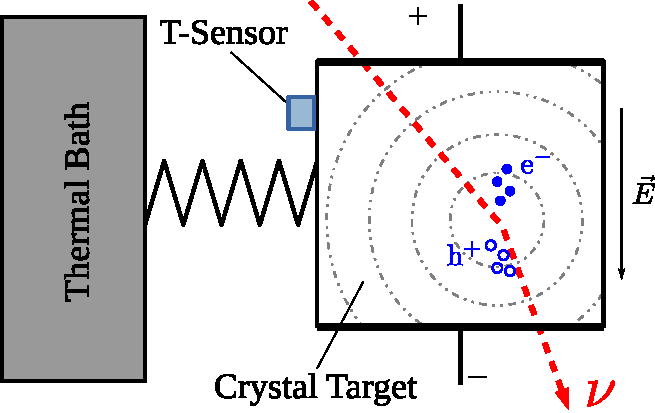
\includegraphics[scale=1]{Figures/Experiment/crystalline_detector_principle.pdf}
\caption{Working principle of a crystalline bolometer (here with additional charge-readout) for particle detection. The induced recoil from an interacting particle (here a nuclear recoil from an incident neutrino) on the atom of the germanium crystal release its recoil energy $E_R$ by creating phonons (illustrated as dashed concentric circles) and excited charge carriers (electron $e^-$ and holes $h^+$). The heat channel measures the increase in temperature $\Delta T$ from the phonons with a GeNTD thermal sensor. The ionization channel consists in the electrodes collecting the drifting charges by applying an electric field $\vec{E}$. Image adapted from \cite{Schumann:2019eaa}}.
\label{fig:detector-principle}
\end{figure}

An ultra-pure semiconductor germanium crystal acts as an absorber: it is the element that serves as a target for the elastic collision of the incident particle. This interaction, called a recoil, deposits a recoil energy $E_R$ in the crystal which is expressed as thermal energy $E_{ph}$ (phonons) and ionization energy $E_{Ion.}$ (electron-hole pairs):
\begin{equation}
\label{energy}
E_R = E_{ph} + E_{Ion.}
\end{equation}

The fraction of the recoil energy going into the phonon and ionization energies is formalized with the quenching factor $Q$ such that:
\begin{equation}
\label{eq:quenching-intro}
E_{Ion.} = Q \cdot E_R \quad \textsf{and} \quad E_{ph} = (1-Q) \cdot E_R
\end{equation}
This quenching factor depends on the type of recoil induced by the incident particle interacting with the germanium crystal. The two major types of recoils considered in this work are the nuclear and the electronic recoils.
The electronic recoils (ER) are generated by incident photons or charged particles. In this case, the particle interacts with the electronic cloud of a germanium atom of the crystal. As a result, the entirety of the recoil energy $E_R$ is expressed in the excitation of the electrons, such that the associated quenching factor is $Q_{ER} = 1$ with $E_{Ion.} = E_R$.
The nuclear recoils (NR), induced by the CENNS process and neutrons, have the incident particle interacting with the nucleus of the atom. The transmitted recoil energy $E_R$ is immediately expressed as gain in momentum of the germanium nucleus. The movement of the nucleus generates vibrations of the crystal lattice, the phonons. The moving nucleus also disturbs the electronic cloud of its atom, thus creating some electron-hole pairs. The quenching factor $Q_{NR}$ associated with the nuclear recoils is an increasing function of the recoil energy $E_R$. It is comprised between 0 and 0.3 for $E_R$ between 0 and \SI{20}{\kilo\eV}.
The intrinsic difference in heat and ionization energies between the nuclear and electronic recoils is the key aspect of the discrimination for the germanium detectors.

% Ionization Channel
The term ionization designates the creation of electron-hole pairs by a recoil. These excited charge carriers are the sole agents of the electric conduction in the semiconducting germanium, each carrying a positive or negative elementary charge $q_e = \SI{1.6e-19}{\coulomb}$.
The ionization energy $E_{e-h}$ determines the number $N_p$ of electron-hole pairs created in the crystal as:
\begin{equation}
E_{Ion.} = N_p \cdot \epsilon_{e^--h^+}
\end{equation}
with $\epsilon_{e^--h^+} \approx \SI{3}{\eV}$ the average energy of a pair in Germanium. 
Several electrodes applying an electric field $\vec{E}$ in the crystal will collect the drifting electrons and holes. The ionization signal is registered as voltage $\Delta V$ in Volt on the electrodes such that:
\begin{equation}
Q = N_p \cdot q_e = C_{el} \Delta V
\end{equation} 
with $Q$ the total collected electric charge in Coulomb and $C_{el}$ the electric capacitance of the electrode in Farad.
The ionization energy $E_{Ion.}$ is deduced from the measured voltage signal $\Delta V$:
\begin{equation}
E_{Ion.} = \frac{C_{el} \cdot \Delta V}{q_{e}} \cdot \epsilon_{e^--h^+}
\end{equation}
and is used to access the recoil energy $E_R$ with knowledge of the quenching in equation \ref{eq:quenching-intro}. This measure of the recoil energy through the ionization energy is defined as the ionization channel of the  detector.


% Phonons, Heat Channel
Phonons are vibrations of the crystal lattice which eventually thermalize with a global increase in temperature of the germanium crystal. The original thermal energy $E_{ph}$ is contained in the phonons created by the recoil and the recombination of the electron-hole pairs, such that $E_{ph} = E_R$.
% NL boost
Additional phonons are produced by the drifting  of the charge carriers across the crystal under the influence of the voltage bias $V_{bias}$ imposed by the electrodes. This process is the Neganov-Trofimov-Luke effect which can be considered as the equivalent of the Joule effect in semiconductors \cite{Luke,Neganov:1985khw}.
The boost to the thermal energy is defined as the Luke-Neganov energy expressed as:
\begin{equation}
E_{NL} = N_p \cdot q_e \cdot V_{bias} = E_{Ion.} \frac{V_{bias}}{\epsilon_{e^--h^+}}
\end{equation}
Hence, the total thermal energy $E_{heat}$ induced by the recoil is expressed:
\begin{equation}
E_{heat} = E_{ph} + E_{NL} = E_R \left( 1 + Q \frac{V_{bias}}{\epsilon_{e^--h^+}} \right)
\end{equation}

It is linked to the increase in crystal temperature $\Delta T$ in Kelvin with the thermal capacity of germanium crystal $C_{Ge}$ in \si{\joule\per\kelvin} such that:
\begin{equation}
E_{heat} = C_{Ge} \cdot \Delta T
\end{equation}
% Thermal leakage
In time, the absorber cools down thanks to the thermal leakage, assured with gold wires between the detector and its copper chassis maintained at constant cryogenic temperature.
% thermistance
This thermal signal can be measured with a very sensitive thermometer. In our case, the thermal sensor is a Neutron transmutation dopped germanium thermistor (GeNTD or NTD) glued on the surface of the crystal. The electric resistance $R_{NTD}$ of this thermistance depends very strongly on its temperature $T_{NTD}$ following the law from Efros and Shllovskii \cite{Mathimalar:2014sfa}:
\begin{equation}
\label{eq:ntd-resistivity}
R_{NTD}(T_{NTD}) = R_0 \cdot \exp(\sqrt{\frac{T_0}{T_{NTD}}})
\end{equation}
where $R_0$ and $T_0$ are a characteristic resistance $\mathcal{O}(1)\ \si{\ohm}$ and temperature $\mathcal{O}(1)\ \si{\kelvin}$ of the NTD used. They depend on the geometry of the NTD and its doping \cite{Mathimalar:2014sfa}. 
Although this thermistor is made of germanium, it is doped and its physical properties are changed: it is conductive and thus has a free electron system in addition to a phonon system. The phonon system has a thermal capacity evolving like the cube of the temperature of the absorber (low thermal capacity), while the capacity of the electron system is linear with the temperature (high thermal capacity). We can therefore understand the usefulness of having an absorber-sensor couple: one serves as a target for the deposition of energy with low thermal capacity, while the other allows the measurement of the temperature rise through the epoxy glue assuring the thermal coupling such that $T_{NTD} \simeq T$.
Therefore, the GeNTD allows the measurement of temperature variations of the germanium crystal with its decreases in resistivity following a particle interaction.
% Polarization
This $R_{NTD}$ resistivity is measured with the polarization of the NTD: a constant direct current $I$ of a few \si{\nano\ampere} is applied to the  thermistance. The Ohm's law gives:
\begin{equation}
\label{eq:ohm-law}
V_{NTD} = R_{NTD} \cdot I
\end{equation}
so that the resistance is deduced from its measured voltage $V_{NTD}$.

% Cryogenic temperature
Cryogenic temperatures are necessary to be in a temperature range where the NTD thermistor becomes sufficiently sensitive to temperature variations. The exponential relation \ref{eq:ntd-resistivity} allows to obtain the largest variation of voltage $\Delta V_{NTD}$ for a small temperature variation $\Delta T$ at the lowest temperature of the detector $T$:
\begin{equation}
\Delta V_{NTD} = 
I \cdot
\left. \frac{\mathrm{d}R_{NTD}}{\mathrm{d}T} \right|_{T}
\cdot
\Delta T
\end{equation}
In the end, the heat energy $E_{heat}$ is derived from the measured voltage signal $\Delta V_{NTD}$ as:
\begin{equation}
E_{heat} = C_{Ge} \cdot \frac{\Delta V_{NTD}}{I} \cdot
\left( \left. \frac{\mathrm{d}R_{NTD}}{\mathrm{d}T} \right|_{T} \right)^{-1}
\end{equation}
It is used to calculate the recoil energy $E_R$ with the knowledge of the quenching $Q$ in equation \ref{eq:quenching-intro}. This measure of the recoil energy through the heat energy is defined as the heat channel of the detector.

% Discrimination
In the end, the cryogenic germanium detectors studied in this work have a double measurement of the recoil energy: the heat channel and the ionization channel. The double read-out is used to discriminate background-induced electron recoils from potential CENNS-induced nuclear recoils on an event-by-event basis.

\begin{figure}
\centering
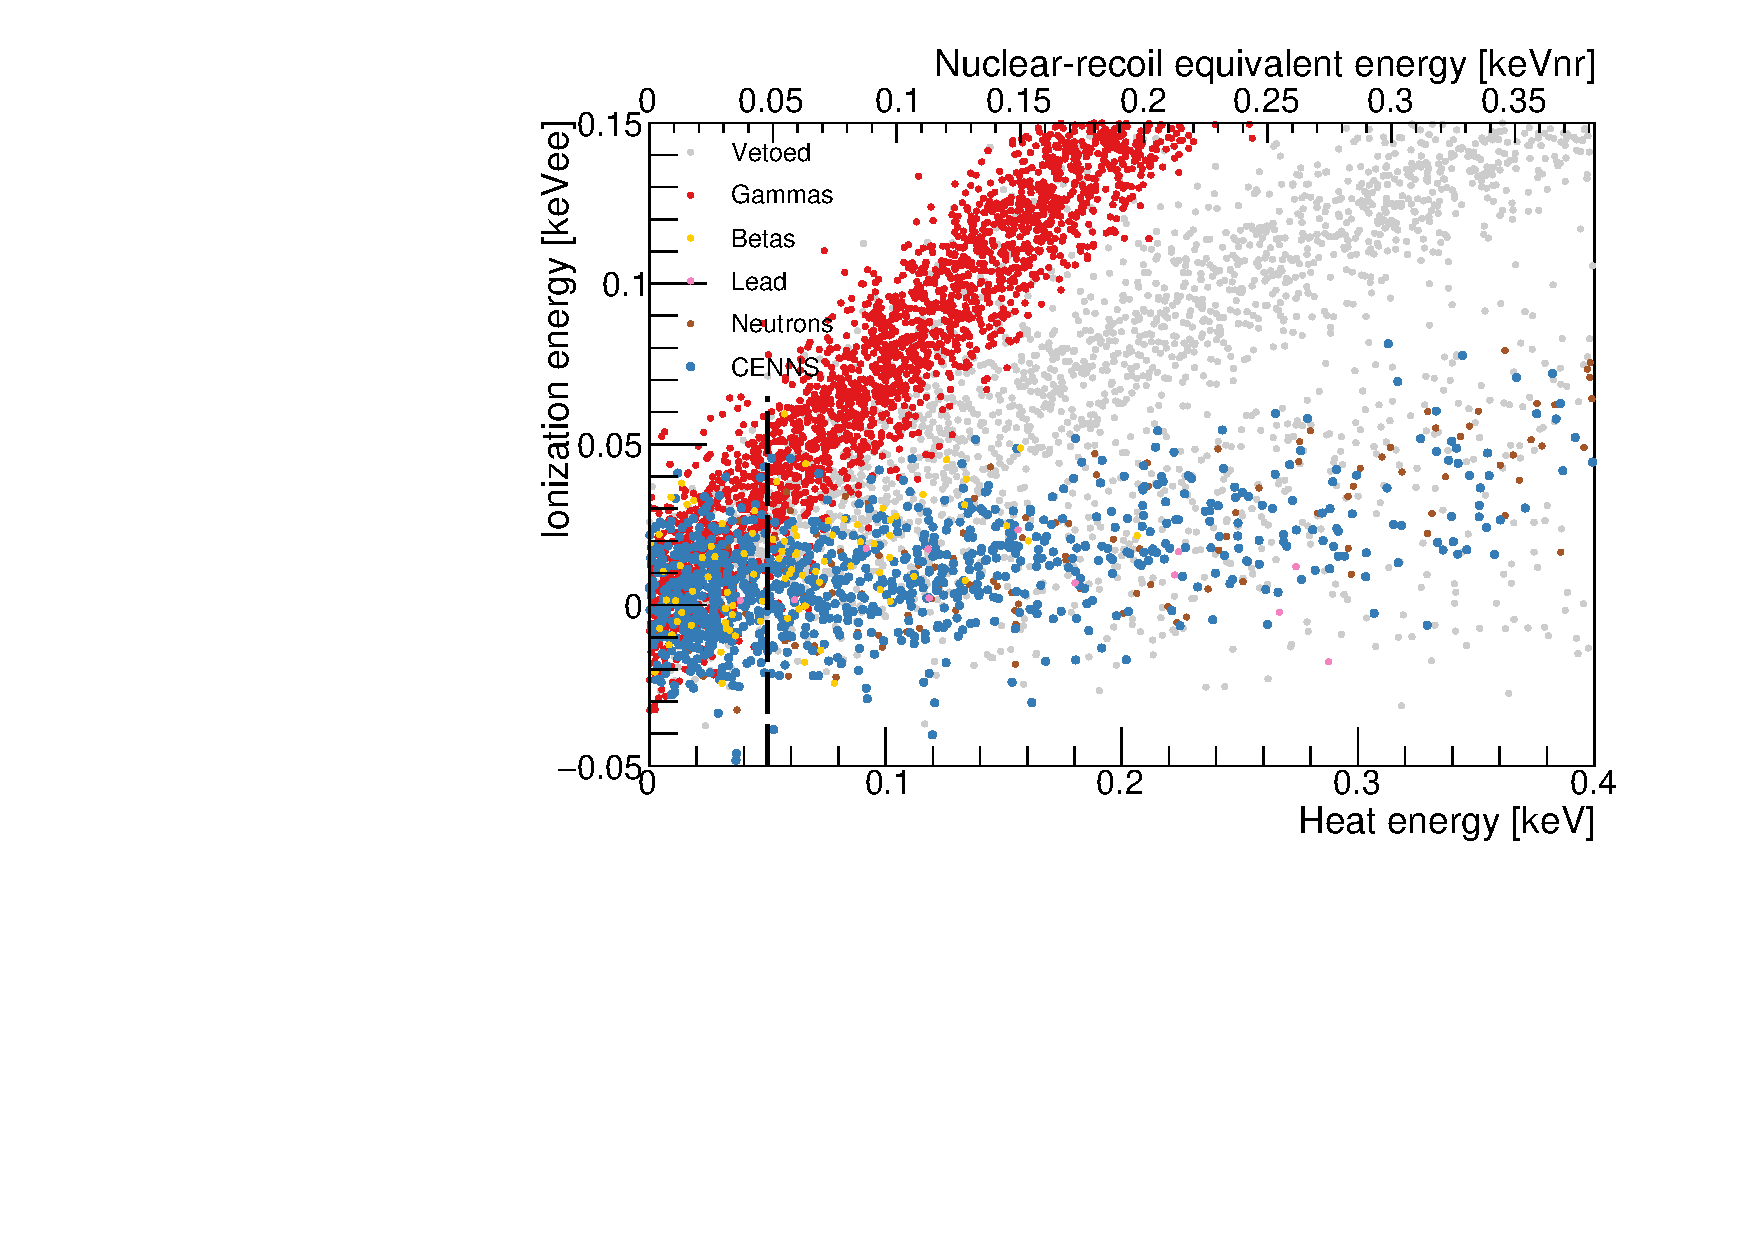
\includegraphics [width=0.7\textwidth]{Figures/Experiment/discrimination_simulation.pdf}
\caption{Illustration of the discrimination of simulated nuclear (blue) and electronic (red) recoils thanks to the simultaneous double-energy measurement with the ionization and heat channels  of the CryoCube detectors. Other type of recoils with negligible event rate are also visible. (Courtesy of J. Billiard)}
\label{fig:discrimination-simulation}
\end{figure}

An illustration of this discrimination is displayed in figure \ref{fig:discrimination-simulation}. The graphic consists in the ionization energy $E_{Ion.}$ versus the heat energy $E_{heat}$ of simulated recoils of different types. Due to their difference in quenching factor $Q_{NR} < Q_{ER}$, the electronic recoils form the red band which is easily separated from the blue band of the nuclear recoils at sufficiently high energy (here for $E_{heat} \geq \SI{0.1}{\kilo\eV}$).  

Hence, the combination of the heat and ionization energies allows a highly efficient rejection of the dominant gamma backgrounds as well as the majority of beta-backgrounds. It is worth highlighting  that, in addition to the event-by-event discrimination, the simultaneous heat and ionization energy measurements also provides a direct measurement of the true nuclear recoil energy, hence avoiding any assumptions on the quenching factor $Q$ to be made. 

%This double-measurement design in a cryogenic bolometer is a characteristic of the \Edelweiss{} experiment and will be in use for \Ricochet{}.



\subsection{RED Prototype Detectors}

% RED series of detectoes
This thesis is inscribed in the R\&D program for the development of the detectors of the CryoCube array. In order to meet its specification presented in paragraph \ref{par:cryocube}, the modelization of the detectors and the subsequent optimization of their design are tested and validated with experimental measurements in the IP2I R\&D cryostat.
These studies are carried out in collaboration with the \Edelweiss{} collaboration with the operation of the RED detector series. The RED series are R\&D-focused bolometers aiming at a full understanding and optimization of the heat and ionization channels. Eventually, the prototypes become very similar to the future element of the CryoCube detector. All of the bolometers discussed hereafter in this work were fabricated by our collaborators at IJCLab, CEA Saclay, and Institut Néel. 

% Crystal shapeand weight
A RED prototype detector is based on cylindrical high-purity Ge crystal weighting between \SI{32}{\g} and \SI{200}{\g}. The crystal is maintained in a copper chassis with Teflon clamps whose heat conduction is negligible compared to the thermal leakage. Every RED detector has a heat channel consisting in one GeNTD thermal sensor glued on the surface of the crystal with gold wires assuring the electric cabling of the NTD and the thermal leakage of the whole detector. 

% Heat Only
In particular, early R\&D detectors such as RED10 and RED20, studied in Chapter \ref{ChapterEthem} were assembled with a very simple and clear design and do not possess an ionization channel. This permits to test thermal models and to better understand the physical processes involved in the thermal response of the detector.

% Electrodes and Ionization channel
Only the most recent RED prototypes, such as RED80 and REDN1 studied in Chapter \ref{ChapterElectrodesExperimental} are equipped with an ionization channel.
The electrodes of these RED detectors are made by evaporating aluminium on the surface of the target material with various shape. It is possible to shape the electric field in the crystal with more complex designs of electrodes. In particular, the detector design FID38, studied Chapter \ref{ChapterElectrodes} and inspired by the FID detectors of \Edelweiss{}-III, has two main collecting electrodes and two auxiliary veto electrodes allowing the tagging of surface events.



% In RED detectors, an energy deposit $\Delta E \sim \si{\kilo\eV}$ induces a temperature variation of the order of \si{\micro\kelvin} and leads to tensions measured from a few hundred \si{\nano\volt}. In practice, the heat signal is modeled by decaying exponential pulses with several characteristics times associated with the different thermalization processes and calorific capacities.


\subsection{Calibration Sources}
\label{par:calibration-source}
\label{par:calibration-sources}

% Calibration source
The detectors are calibrated with particles inducing recoils of known heat ($E_{heat}$) and the ionization ($E_{Ion.}$) energies.
% Cosmic muons
For the first RED detectors, cosmic muons of high energy were used as calibration source. This natural source, available due to the very low overburden of the cryogenic facility, would generate a large ionization peak at \SI{18}{\mega\eV}. This calibration source has significant uncertainty on the position of the peak due to the wide cosmic muon energy distribution. Also, due to the non-linearity of the heat response, the measurements at low energies are severely underestimated with this calibration at high energy.

% Iron source
The muon calibration was quickly replaced with the use of radioactive iron sources.
An $^{55}$Fe calibration source was glued on the inner part of the detector's copper housing and facing the crystal surface opposite to the side on which is glued the GeNTD. It generates electronic recoils from a doublet peak of X-ray emission at \SI{5.90}{\kilo\eV} and \SI{6.49}{\kilo\eV}. This calibration method was mainly used for the operation of the RED detectors equipped solely with a heat channel (RED10 and RED20 in this work).

% activated germanium
The newest and most advantageous calibration method used in the current runs at IP2I is based on the activation of the germanium atoms in the crystal of the detectors with thermal neutrons. The detectors are activated with an intense AmBe neutron source, inducing the neutron capture by the stable \ce{{}^{70}Ge}:
\begin{equation}
\ce{{}^{70}Ge + n -> {}^{71}Ge}
\end{equation}
The \ce{^{70}Ge} isotope decays \cite{Abusaleem:2011} through electron capture with the half-life $t_{1/2} = \SI{11.43}{\day}$ as:
\begin{equation}
\ce{^{71}Ge + e^- -> {}^{71}Ga^* + $\nu$_e}
\end{equation}
The daughter nucleus \ce{{}^{71}Ga^*} is in an excited state due to the hole left in one of its electronic shell. When relaxing, a photon is emitted which produces an electronic recoil in the germanium crystal of the detector. The energy of this photon is equal to the binding energy of the electron associated with the K/L/M shells of the \ce{{}^{71}Ga}: \SI{10.37}{\kilo\eV}, \SI{1.3}{\kilo\eV} and \SI{160}{\eV} respectively \cite{thompson2001x}. All these calibration peaks are in the exact energy range for the CENNS signal search $\mathcal{O}(1)$\si{\kilo\eV} while yielding a uniform distribution of the recoils in the whole detector volume. A direct application of this property is the experimental estimation of the fiducial volume and efficiency of the RED detectors as described in Chapter \ref{ChapterElectrodesExperimental}.


% activated germanium
%The newest and most advantageous calibration method used in the current runs at IP2I is based on the activation of the $^{71}$Ge in the crystal of the detectors with thermal neutrons. The detectors are activated with an intense AmBe neutron source. As such, the germanium crystal acts as a radioactive source generating electronics recoils from the X-ray emission of the K/L/M shells of the germanium. These peaks are located at recoil energies of \SI{10.37}{\kilo\eV}, \SI{1.3}{\kilo\eV} and \SI{160}{\eV} respectively. All these calibration peaks are in the exact energy range for the CENNS signal search $\mathcal{O}(1)$\si{\kilo\eV} while yielding a uniform distribution of the recoils in the whole detector volume. A direct application of this property is the experimental estimation of the fiducial volume and efficiency of the RED detectors as described in Chapter \ref{ChapterElectrodesExperimental}.


%----------------------------------------------------------------------------------------
%	BONUS UNUSED
%----------------------------------------------------------------------------------------

%\section{Detector principle}
%
%\begin{equation}
%\begin{cases}
%Q = Q_{ER} = 1 \\
%E_{Ion.}^{bulk} = Q \cdot E_R = E_R \\
%E_{heat} 
%=
%E_R 
%\cdot
%\frac{
%1 + Q_{ER}\frac{V_{bias}}{\epsilon_{e^--h^+}}
%}{
%1 + \frac{V_{bias}{\epsilon_{e^--h^+}}
%}
%= E_R
%\end{cases}
%\end{equation}
%
%\begin{equation}
%\begin{cases}
%Q = Q_{NR} \left( E_R \right) \\
%E_{Ion.}^{bulk} = Q_{NR}\left( E_R \right) \cdot E_R \\
%E_{heat} 
%=
%E_R 
%\cdot
%\frac{
%1 + Q_{NR} \left( E_R \right)\frac{V_{bias}}{\epsilon_{e^--h^+}}
%}{
%1 + \frac{V_{bias}{\epsilon_{e^--h^+}}
%}
%\end{cases}
%\end{equation}
%
%\begin{equation}
%\begin{cases}
%Q = Q_{HO} = 0 \\
%E_{Ion.}^{bulk} = Q_{NHO} \cdot E_R = 0 \\
%E_{heat} 
%=
%E_R 
%\cdot
%\frac{
%1 + Q_{HO} \left( E_R \right)\frac{V_{bias}}{\epsilon_{e^--h^+}}
%}{
%1 + \frac{V_{bias}{\epsilon_{e^--h^+}}
%}
%=
%E_R 
%\cdot
%\frac{
%1
%}{
%1 + \frac{V_{bias}{\epsilon_{e^--h^+}}
%}
%\end{cases}
%\end{equation}


%% Heat Channel Study
%% Chapter Ethem

\chapter{Electro-Thermal Modelization of the RED Dectectors}

\label{ChapterEthem} % Change X to a consecutive number; for referencing this chapter elsewhere, use \ref{ChapterX}

%----------------------------------------------------------------------------------------
%	BEGING CHAPTER
%----------------------------------------------------------------------------------------

\section{Basic Modelization of Cryogenic Bolometers}

Even though the design of the RED bolometers is quite simple, a complete modelization of its behavior requires quite some time and efforts. However, it is possible to gain some insight from a very simplified modelization (see fig \ref{bolo-model}): we consider a single thermal bath of thermal capacity $C$ and temperature $T$ thermalized by a conductance $G$ to the cryostat at temperature $T_{cryo}$. We consider the temperature of the NTD resistance $R$ to be $T$. With a constant polarization current $I$, the NTD delivers a Joule power $P_J = RI^2$ into the bolometer and the voltage $V=RI$ is amplified by the FET-based electronic. It should be noted that the constant current $I$ is obtained by passing a triangular voltage wave through an electric capacity (this presents some advantages, more will be discuss).

\begin{figure}
\centering
\captionsetup{justification=centering}
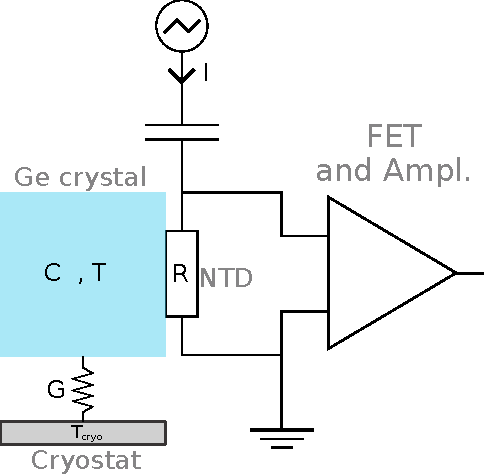
\includegraphics[width=0.3\textwidth]{graphics/bolo_simple.pdf}
\caption{\label{bolo-model} \em Simplified scheme of a RED bolometer coupling a thermal system (left side) and an electrical system (right side). }
\end{figure}

Here are some hints and info to help you understand the behavior of the bolometers (calculation and discussion in parallel with the measurements):
\begin{itemize}
	\item The heat power injected by the cryostat into the bolometer is $$P_{cryo} = G \left( T_{cryo} - T\right) \quad [\textrm{in } Watt]$$ In the considered simplified system, only the limiting conductance is considered (the lowest) which is generally the electron-phonon coupling (more in discussion..)
	\item A lot can be understand from studying the stationary state ($dT/dt=0$) and the time resolution (useful to introduce $\Delta T = T - T_{eq}$) of the heat equilibrium equation in the stationary state. Just recall that with $t$ the time and $U$ the energy of the thermal bath $$\frac{dU}{dt} = C \frac{dT}{dt} \quad [\textrm{in }  Joule]$$
	\item Some reference value for RED bolometers:
	$$ R = \mathcal{O}(1 \ G\Omega),\
	C \approx 3 \times 10^{-10} \ J.K^{-1},\
	G \approx 2 \times 10^{-8} \ W.K^{-1},\
	I = \mathcal{O}(1 \ nA),\
	T_{cryo} \approx 20 \ mK $$
	\item An optimized bolometer has the highest sensitivity $S_V$ in V/keV possible. Not to confuse with the sensitivity of the thermal sensor $\alpha$ which is usually introduced in this type of calculation 
	$$\alpha = \frac{1}{R} \frac{dR}{dT} $$
\end{itemize}


\subsection{Electro-thermal Modelization of the Detector}

In this part, the theoretical calculations used to build the detector model are presented. The study focused on the first-order resolution of the system of coupled differential equations using a linear algebra method : \cite{matrix}. It is then possible to simulate the behavior of a detector in the steady state, in the time regime and in the frequency regime, which gives access to the complete characterization of the detector.


\subsection{Model description}

\begin{figure}[!ht]
%\centering
%\resizebox{0.6\textwidth}{!}{%
%\shorthandoff{:!}\begin{circuitikz}[scale=1]
%	%	\draw [help lines, step=0.5cm] (0.25,0) grid (7.75,5);
	\node [below] at (4, 0.05) {$T_b$};
	\fill [pattern = north east lines] (2.5,0.05) rectangle (5.5,0.25);
	\draw [brown, line width = 5] (4,0.25) -- (4,1.75);
	\draw [thick] (2.5,0.25) -- (5.5,0.25);
	\draw [brown, line width = 5] (3.25, 2.5) -- (1.75, 2.5);
	\draw [brown, line width = 5] (4.75, 2.5) -- (6.25, 2.5);
	\node [right] at (4, 1)	{$G_{pb}$};
	\node [left] at (4, 1)	{$P_{pb}$};
	\node [below] at (2.5, 2.5)	{$G_{ap}$};
	\node [above] at (2.5, 2.5)	{$P_{ap}$};
	\node [below] at (5.5, 2.5)	{$G_{ep}$};
	\node [above] at (5.5, 2.5)	{$P_{ep}$};
	\draw [fill=yellow] (3.25, 1.75) rectangle (4.75, 3.25);
	\node at (4, 2.5) {$T_p, C_p$};
	\draw [fill=orange] (1.75, 1.75) rectangle (0.25, 3.25);
	\node at (1, 2.5) {$T_a, C_a$};
	\draw [fill=cyan] (6.25, 1.75) rectangle (7.75, 3.25);
	\node at (7, 2.5) {$T_e, C_a$};
	\node [anchor=south, inner sep=0] at (1, 3.5)
    	{\resizebox{2cm}{!}{% This file was created by matplotlib2tikz v0.6.10.
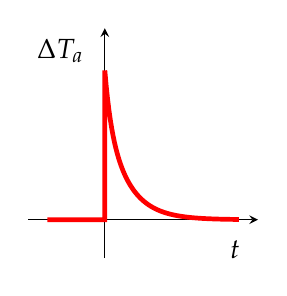
\begin{tikzpicture}

\begin{axis}[
ticks=none,
xmin=-0.2, xmax=0.4,
ymin=-0.5e-07, ymax=2.5e-07,
axis x line=center,
axis y line=center,
every axis x label/.style={at={(ticklabel cs:0.9)}, below=4pt},
every axis y label/.style={at={(ticklabel cs:0.9)}, left=4pt},
xlabel={$t$},
ylabel={$\Delta T_a$},
width=4.5cm,
height=4.5cm
]
\addplot [line width = 1.7pt, red]
table {%
-0.15 0
1e-08 0
0 1.94905773450583e-07
0.00353535353535354 1.75086151002447e-07
0.00707070707070707 1.58214334725911e-07
0.0106060606060606 1.4370498349366e-07
0.0141414141414141 1.31131841539708e-07
0.0176767676767677 1.20154073651191e-07
0.0212121212121212 1.10498558052284e-07
0.0247474747474747 1.01945886553252e-07
0.0282828282828283 9.43192935859211e-08
0.0318181818181818 8.74758993005682e-08
0.0353535353535354 8.1299781085828e-08
0.0388888888888889 7.56964899078769e-08
0.0424242424242424 7.05887084549368e-08
0.045959595959596 6.59128117256344e-08
0.0494949494949495 6.16161409749693e-08
0.053030303030303 5.76548416413408e-08
0.0565656565656566 5.39921472429897e-08
0.0601010101010101 5.05970160062528e-08
0.0636363636363636 4.74430465564955e-08
0.0671717171717172 4.45076144595586e-08
0.0707070707070707 4.17711836111647e-08
0.0742424242424242 3.92167561164711e-08
0.0777777777777778 3.68294319208594e-08
0.0813131313131313 3.45960554718693e-08
0.0848484848484848 3.25049314471608e-08
0.0883838383838384 3.05455953401098e-08
0.0919191919191919 2.8708627662862e-08
0.0954545454545454 2.69855028720667e-08
0.098989898989899 2.53684659759339e-08
0.102525252525253 2.38504312460595e-08
0.106060606060606 2.24248986152695e-08
0.10959595959596 2.10858842580303e-08
0.113131313131313 1.98278625736718e-08
0.116666666666667 1.86457173650087e-08
0.12020202020202 1.75347004576861e-08
0.123737373737374 1.64903963638234e-08
0.127272727272727 1.55086918770988e-08
0.130808080808081 1.45857497109756e-08
0.134343434343434 1.37179854696812e-08
0.137878787878788 1.29020473825878e-08
0.141414141414141 1.21347983445272e-08
0.144949494949495 1.14132998934018e-08
0.148484848484848 1.07347978270466e-08
0.152020202020202 1.00967092174591e-08
0.155555555555556 9.49661062525964e-09
0.159090909090909 8.93222735294378e-09
0.162626262626263 8.40142360402661e-09
0.166161616161616 7.9021934380375e-09
0.16969696969697 7.43265242968028e-09
0.173232323232323 6.99102995525483e-09
0.176767676767677 6.57566204137687e-09
0.18030303030303 6.18498472071477e-09
0.183838383838384 5.81752784734487e-09
0.187373737373737 5.4719093307749e-09
0.190909090909091 5.14682975298612e-09
0.194444444444444 4.84106733722839e-09
0.197979797979798 4.5534732409492e-09
0.201515151515152 4.28296714829148e-09
0.205050505050505 4.02853314017069e-09
0.208585858585859 3.78921582212947e-09
0.212121212121212 3.56411669204082e-09
0.215656565656566 3.35239073134553e-09
0.219191919191919 3.15324320491336e-09
0.222727272727273 2.96592665584594e-09
0.226262626262626 2.78973808262336e-09
0.22979797979798 2.62401628695844e-09
0.233333333333333 2.46813938158316e-09
0.236868686868687 2.32152244796522e-09
0.24040404040404 2.18361533465225e-09
0.243939393939394 2.05390058757701e-09
0.247474747474747 1.93189150423773e-09
0.251010101010101 1.81713030419968e-09
0.254545454545455 1.70918640885407e-09
0.258080808080808 1.6076548238223e-09
0.261616161616162 1.51215461781191e-09
0.265151515151515 1.42232749211878e-09
0.268686868686869 1.3378364353309e-09
0.272222222222222 1.2583644581251e-09
0.275757575757576 1.18361340336156e-09
0.279292929292929 1.11330282697358e-09
0.282828282828283 1.04716894542388e-09
0.286363636363636 9.84963645754594e-10
0.28989898989899 9.26453554498324e-10
0.293434343434343 8.71419161942022e-10
0.296969696969697 8.19653998446613e-10
0.30050505050505 7.70963859722854e-10
0.304040404040404 7.25166078149621e-10
0.307575757575758 6.82088837395062e-10
0.311111111111111 6.41570527764773e-10
0.314646464646465 6.03459139854875e-10
0.318181818181818 5.67611694232354e-10
0.321717171717172 5.33893705000791e-10
0.325252525252525 5.02178675237199e-10
0.328787878787879 4.72347622405636e-10
0.332323232323232 4.44288631966024e-10
0.335858585858586 4.17896437502591e-10
0.339393939393939 3.93072025796083e-10
0.342929292929293 3.69722265357532e-10
0.346464646464646 3.47759557029615e-10
0.35 3.27101505344391e-10
};
\end{axis}

\end{tikzpicture}}};
    \node [anchor=south, inner sep=0] at (4, 3.5)
    	{\resizebox{2cm}{!}{% This file was created by matplotlib2tikz v0.6.10.
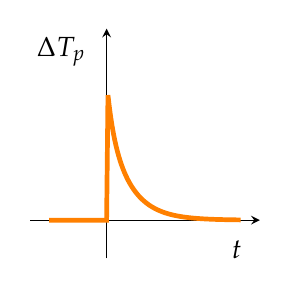
\begin{tikzpicture}

\definecolor{color0}{rgb}{1,0.647058823529412,0}


\begin{axis}[
ticks=none,
xmin=-0.2, xmax=0.4,
ymin=-0.5e-07, ymax=2.5e-07,
axis x line=center,
axis y line=center,
every axis x label/.style={at={(ticklabel cs:0.9)}, below=4pt},
every axis y label/.style={at={(ticklabel cs:0.9)}, left=4pt},
xlabel={$t$},
ylabel={$\Delta T_p$},
width=4.5cm,
height=4.5cm
]
\addplot [line width = 1.7pt, orange]
table {%
-0.15 0
1e-08 0
0 6.96368541805659e-24
0.00353535353535354 1.63176399143611e-07
0.00707070707070707 1.48010174769528e-07
0.0106060606060606 1.34895295323391e-07
0.0141414141414141 1.23468086776223e-07
0.0176767676767677 1.13437308330477e-07
0.0212121212121212 1.04569165237934e-07
0.0247474747474747 9.6675457798133e-08
0.0282828282828283 8.96042081124974e-08
0.0318181818181818 8.32322445633661e-08
0.0353535353535354 7.74593332500688e-08
0.0388888888888889 7.22035319129691e-08
0.0424242424242424 6.73975100378826e-08
0.045959595959596 6.29856326697683e-08
0.0494949494949495 5.89216479870297e-08
0.053030303030303 5.51668522742115e-08
0.0565656565656566 5.16886324595516e-08
0.0601010101010101 4.8459307338149e-08
0.0636363636363636 4.54552051530634e-08
0.0671717171717172 4.26559282807991e-08
0.0707070707070707 4.00437660952089e-08
0.0742424242424242 3.76032252420987e-08
0.0777777777777778 3.53206530016271e-08
0.0813131313131313 3.31839345070543e-08
0.0848484848484848 3.11822486108937e-08
0.0883838383838384 2.93058703676763e-08
0.0919191919191919 2.75460106137664e-08
0.0954545454545454 2.58946851090798e-08
0.098989898989899 2.43446072738405e-08
0.102525252525253 2.28890997930618e-08
0.106060606060606 2.15220213413162e-08
0.10959595959596 2.02377054550822e-08
0.113131313131313 1.90309091926043e-08
0.116666666666667 1.78967697058042e-08
0.12020202020202 1.68307672321937e-08
0.123737373737374 1.58286933182089e-08
0.127272727272727 1.48866233256637e-08
0.130808080808081 1.40008924633649e-08
0.134343434343434 1.31680747367947e-08
0.137878787878788 1.23849643284248e-08
0.141414141414141 1.16485590162039e-08
0.144949494949495 1.0956045313217e-08
0.148484848484848 1.0304785071529e-08
0.152020202020202 9.69230334102103e-09
0.155555555555556 9.11627731213953e-09
0.159090909090909 8.57452620193543e-09
0.162626262626263 8.06500196714538e-09
0.166161616161616 7.58578074763144e-09
0.16969696969697 7.13505495923382e-09
0.173232323232323 6.71112596779503e-09
0.176767676767677 6.31239728640301e-09
0.18030303030303 5.93736824626804e-09
0.183838383838384 5.58462809848333e-09
0.187373737373737 5.25285050953076e-09
0.190909090909091 4.94078841802559e-09
0.194444444444444 4.64726922404115e-09
0.197979797979798 4.37119028557055e-09
0.201515151515152 4.111514699389e-09
0.205050505050505 3.86726734587531e-09
0.208585858585859 3.63753117931072e-09
0.212121212121212 3.4214437468602e-09
0.215656565656566 3.21819392090423e-09
0.219191919191919 3.02701883066689e-09
0.222727272727273 2.84720098021137e-09
0.226262626262626 2.67806554087111e-09
0.22979797979798 2.51897780707433e-09
0.233333333333333 2.36934080531901e-09
0.236868686868687 2.2285930467763e-09
0.24040404040404 2.09620641465547e-09
0.243939393939394 1.97168417806043e-09
0.247474747474747 1.85455912461491e-09
0.251010101010101 1.74439180463596e-09
0.254545454545455 1.64076888009906e-09
0.258080808080808 1.54330157206693e-09
0.261616161616162 1.45162420065171e-09
0.265151515151515 1.36539281194944e-09
0.268686868686869 1.28428388672967e-09
0.272222222222222 1.20799312598366e-09
0.275757575757576 1.13623430873391e-09
0.279292929292929 1.06873821778733e-09
0.282828282828283 1.00525162937641e-09
0.286363636363636 9.45536362877567e-10
0.28989898989899 8.89368387025501e-10
0.293434343434343 8.36536979257968e-10
0.296969696969697 7.86843935027003e-10
0.30050505050505 7.4010282410245e-10
0.304040404040404 6.96138291071478e-10
0.307575757575758 6.54785397404927e-10
0.311111111111111 6.15889002618282e-10
0.314646464646465 5.79303182202572e-10
0.318181818181818 5.44890680139068e-10
0.321717171717172 5.12522393941935e-10
0.325252525252525 4.82076890295391e-10
0.328787878787879 4.53439949467044e-10
0.332323232323232 4.26504136787296e-10
0.335858585858586 4.01168399586413e-10
0.339393939393939 3.77337688076548e-10
0.342929292929293 3.5492259875595e-10
0.346464646464646 3.33839038997186e-10
0.35 3.14007911560752e-10
};
\end{axis}

\end{tikzpicture}}};	
    \node [anchor=south, inner sep=0] at (7, 3.5)
    	{\resizebox{2cm}{!}{% This file was created by matplotlib2tikz v0.6.10.
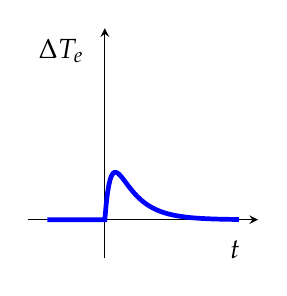
\begin{tikzpicture}

\begin{axis}[
ticks=none,
xmin=-0.2, xmax=0.4,
ymin=-0.5e-07, ymax=2.5e-07,
axis x line=center,
axis y line=center,
every axis x label/.style={at={(ticklabel cs:0.9)}, below=4pt},
every axis y label/.style={at={(ticklabel cs:0.9)}, left=4pt},
xlabel={$t$},
ylabel={$\Delta T_e$},
width=4.5cm,
height=4.5cm
]
\addplot [line width = 1.7pt, blue]
table {%
-0.15 0
1e-08 0
0 5.15986218822629e-23
0.00353535353535354 2.02319742455945e-08
0.00707070707070707 3.50283638973746e-08
0.0106060606060606 4.55829895717481e-08
0.0141414141414141 5.2854683483701e-08
0.0176767676767677 5.75967408445595e-08
0.0212121212121212 6.04003591661948e-08
0.0247474747474747 6.17289341324563e-08
0.0282828282828283 6.19451332621564e-08
0.0318181818181818 6.13322662511764e-08
0.0353535353535354 6.0111151566108e-08
0.0388888888888889 5.84534266690334e-08
0.0424242424242424 5.64920500734984e-08
0.045959595959596 5.4329586121974e-08
0.0494949494949495 5.20447391339915e-08
0.053030303030303 4.96975054505508e-08
0.0565656565656566 4.73332344043295e-08
0.0601010101010101 4.49858280406682e-08
0.0636363636363636 4.26802610766907e-08
0.0671717171717172 4.04345644105182e-08
0.0707070707070707 3.82613853431711e-08
0.0742424242424242 3.6169213865249e-08
0.0777777777777778 3.41633455563404e-08
0.0813131313131313 3.22466367949145e-08
0.0848484848484848 3.04200962489964e-08
0.0883838383838384 2.86833473567554e-08
0.0919191919191919 2.70349891927568e-08
0.0954545454545454 2.54728773405602e-08
0.098989898989899 2.39943418321705e-08
0.102525252525253 2.25963556141392e-08
0.106060606060606 2.12756641571379e-08
0.10959595959596 2.00288845812559e-08
0.113131313131313 1.88525808972803e-08
0.116666666666667 1.77433205654116e-08
0.12020202020202 1.66977164687768e-08
0.123737373737374 1.571245752772e-08
0.127272727272727 1.4784330493241e-08
0.130808080808081 1.39102349154358e-08
0.134343434343434 1.30871928548508e-08
0.137878787878788 1.23123545671688e-08
0.141414141414141 1.15830011255645e-08
0.144949494949495 1.0896544735358e-08
0.148484848484848 1.02505273303853e-08
0.152020202020202 9.64261791040749e-09
0.155555555555556 9.07060897650632e-09
0.159090909090909 8.53241234089511e-09
0.162626262626263 8.02605452431492e-09
0.166161616161616 7.54967190452406e-09
0.16969696969697 7.10150574045727e-09
0.173232323232323 6.67989716615275e-09
0.176767676767677 6.2832822247284e-09
0.18030303030303 5.91018699411838e-09
0.183838383838384 5.55922284183937e-09
0.187373737373737 5.2290818348624e-09
0.190909090909091 4.91853232202482e-09
0.194444444444444 4.62641469977975e-09
0.197979797979798 4.35163736701518e-09
0.201515151515152 4.09317287084003e-09
0.205050505050505 3.85005424236218e-09
0.208585858585859 3.62137151936202e-09
0.212121212121212 3.40626845122712e-09
0.215656565656566 3.20393938043e-09
0.219191919191919 3.01362629409614e-09
0.222727272727273 2.83461603874513e-09
0.226262626262626 2.66623769102869e-09
0.22979797979798 2.50786007718652e-09
0.233333333333333 2.35888943395577e-09
0.236868686868687 2.21876720377107e-09
0.24040404040404 2.08696795725728e-09
0.243939393939394 1.96299743622671e-09
0.247474747474747 1.84639071063342e-09
0.251010101010101 1.73671044319756e-09
0.254545454545455 1.63354525568494e-09
0.258080808080808 1.53650819110403e-09
0.261616161616162 1.44523526636046e-09
0.265151515151515 1.359384110183e-09
0.268686868686869 1.27863268140426e-09
0.272222222222222 1.20267806293949e-09
0.275757575757576 1.13123532705958e-09
0.279292929292929 1.06403646779599e-09
0.282828282828283 1.00082939654757e-09
0.286363636363636 9.41376997180387e-10
0.28989898989899 8.85456237122462e-10
0.293434343434343 8.32857331155583e-10
0.296969696969697 7.83382954796269e-10
0.30050505050505 7.36847504337837e-10
0.304040404040404 6.93076400795766e-10
0.307575757575758 6.51905435159421e-10
0.311111111111111 6.13180152505136e-10
0.314646464646465 5.76755272669063e-10
0.318181818181818 5.42494145313467e-10
0.321717171717172 5.10268237347692e-10
0.325252525252525 4.79956650785216e-10
0.328787878787879 4.51445669231489e-10
0.332323232323232 4.24628331303897e-10
0.335858585858586 3.9940402938568e-10
0.339393939393939 3.75678132210213e-10
0.342929292929293 3.53361629861074e-10
0.346464646464646 3.32370799857171e-10
0.35 3.12626893071057e-10
};
\end{axis}

\end{tikzpicture}}};
    	
%\end{circuitikz}\shorthandon{:!}
%}%
\begin{center}
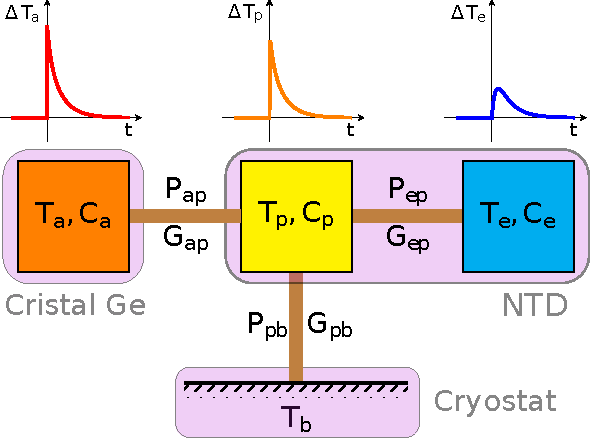
\includegraphics[width=0.6\textwidth]{Images/thermal_scheme.pdf}
\end{center}
\caption{Thermal diagram of RED1 and RED10 with representation of the diffusion of a signal created by an event in the germanium crystal. Each thermal bath is characterized by a temperature $T$ and a thermal capacity $C$. Each thermal link is associated with a thermal conductivity $G$ and a thermal power transfer $P$. The NTD sensor is modeled as a system of thermally coupled phonons (index $p$) and elecrons (index $e$). The absorber bath (index $a$) and the cryostat (index $b$) are both connected to the NTD phonon bath.}
\label{thermal-scheme}
\end{figure}

\begin{figure}[!ht]
\begin{minipage}[c]{0.45\textwidth}
\resizebox{!}{\textwidth}{%
%\shorthandoff{:!}
\begin{circuitikz}[scale=1]
	  	\draw
	 (0.5,6) node [ground, rotate=-90] {} 
	 to [european voltage source, v=$V_B$, -*] (2,6)
	 to [european voltage source, l={\color{red} $e_{J_{RL}}$}, color=red] (2,4.5)	 
	 to [R, l_=$R_L$, -] (2,2.5)
	 to [thR, l_=$R(T_e)$, -] (2,0.5)
	 to [european voltage source, l={\color{red} $e_{J_{NTD}}$}, color=red]
	  (2,-0.5) node [ground] {}
	 (2,2.5) to [short, -o] (4,2.5) node [anchor=south] {$V$}
	 to [C, l_=$C_{fil}$] (4,-0.5) node [ground] {} 
	 (4,2.5) to [european voltage source, l={\color{red} $e_{ampli.}$}, color=red] (6,2.5) 
	 to [ioosource, l={\color{red} $i_{ampli.}$}, color=red] (6,-0.5) node [ground] {} 
	 (6,2.5) node [anchor=south] {$U$}
	 to [short, i_={\small $i \approx 0$}, *-] (7,2.5)
	 to [amp, l=Suiveur, -] (8,2.5)
	;
\end{circuitikz}
%\shorthandon{:!}
}%
\end{minipage}
\hfill
\vrule{}
\hfill
\begin{minipage}[c]{0.45\textwidth}
\begin{center}
avec Thèvenin-Norton, en fréquentiel :
\end{center}
\resizebox{\textwidth}{!}{%
%\shorthandoff{:!}
\begin{circuitikz}
		\draw
	 (0,0) node [ground] {}
	 to [R, l_=$Z_{eq}$, -] (0,2)
	 (0,2) to [short, -o] (2,2) node [anchor=south] {$V$}
	 to [ioosource, l=$\color{red} i_{bruit}$,color=red, -] 
	 (2,0) node [ground] {}
	 (2,2) to [european voltage source, l={\color{red} $e_{ampli.}$}, color=red, -] (4,2) node [anchor=south] {$U$}
	 to [short, i_={\small $i \approx 0$}, *-] (5,2)
	 to [amp, l=Suiveur, -] (6,2)
	 (0,-1.5) node [right]{$\color{red} \displaystyle i_{bruit}^2=\left(\frac{e_{J_{NTD}}}{R(T_e)}\right)^2+\left(\frac{e_{J_{R_L}}}{R_L}\right)^2+i_{ampli.}^2$}
	;
\end{circuitikz}
%\shorthandon{:!}
}%
\end{minipage}
\caption{Diagrams of the polarization electronics. The NTD resistor $R(T_e)$, the load resistor $R_L$ and the wiring capacitance $C_{wire}$ become the equivalent complex impedance $Z_{eq}$. Noise sources appear in red. Johnson noise, $e_{J_{RL}}$ and $e_{J_{NTD}}$, and amplifier current noise $i_{ampli.}$ are grouped into a current noise $i_{noise}$ whose expression is specified.}
\label{electric-scheme}
\end{figure}

The approximation of a system of three thermal baths is used to model a RED detector \cite{note}. The thermal scheme of a detector in such an approximation is presented in the \hyperref[thermal-scheme]{Figure 1}. This model best models a germanium crystal absorber on which a single NTD thermal sensor is glued. As shown in the \hyperref[thermal-scheme]{Figure 1}, there are three thermal baths, each characterized by a thermal capacity $C$ and a temperature $T$ :
\begin{itemize}
\item in orange, the germanium crystal acting as an absorber ($T_a$, $C_a$),
\item in yellow, the thermal bath of the phonons in the NTD resistor ($T_p$, $C_p$),
\item in blue, the thermal bath of electrons in the NTD resistor ($T_e$, $C_e$).
\end{itemize}
They are connected by thermal links characterized by thermal conductivity $G$, which allows a power transfer $P$ between the baths. There is also the presence of a thermal leakage from the NTD resistor to the cryostat (in black dashes) which allows to set an operating temperature $T_b$.
In order to measure the NTD resistance variation, generated by an energy deposit within the detector during an interaction with a particle, it is necessary to polarize the sensor in current. This is done by adding a very high load resistance in series. The NTD sensor is then traversed by an almost constant $I_P$ bias current during an event. The electronic schematic that allows the polarization and the measurement of the voltage $V$ at the terminals of the NTD resistor is shown in the figure \ref{electric-scheme}. There is on the left the schematic of the polarization electronics with noise representation (in red) and on the right the simplification of the schematic by Thevenin-Norton transformation \cite{mather} in the context of the frequency study, which will come later. A constant bias voltage $V_B$ is applied to the load resistance $R_L$, of a few $G\Omega$, in series with the NTD resistance $R(T_e)$ depending on the temperature of the electron bath. The capacity of the wiring $C_{wire}$ of the electronics is taken into account.

In order to predict the response of the detector to an event, this electro-thermal model must now be solved. We then define the system of differential equations coupled by the power exchange between the thermal baths, and with the electronic system by the Joule power induced by the bias current within the NTD sensor.

For the electron system of the NTD, we first have a power from the Joule effect $P_J= I_P^2 R(T_e)=\frac{V^2}{R(T_e)}$. Then we have the power transfer from the phonon system of the NTD expressed as: $P_{ep}=V_{NTD} g_{ep} (T_e^n - T_p^n)$ where $V_{NTD}$ is the volume of the NTD sensor, $g_{ep}$ is the electron-phonon coupling constant per unit volume and $n$ is a material dependent exponent that is typically 6 for thermistors such as germanium NTDs. The thermal equilibrium equation for the electron bath is,
\begin{equation}
\label{electron}
 C_e \frac{d T_e}{d t} = \frac{V^2}{R(T_e)} - V_S g_{ep} \left( T_e^{n} - T_p^{n} \right)
\end{equation}

For the absorber, the thermal bath represents only the phonon system of the germanium crystal. Since this material is a semiconductor material in the form of an ultra-pure crystal, there are no free electrons. The absorber exchanges a power with the phonon system of the NTD by considering the thermal capacity of the glue to be negligible. This is written $P_{ap}=g_{glue} S_{NTD} \left( T_p^{n_g} - T_a^{n_g} \right)$ with $S_{NTD}$ the surface of the NTD bonded to the absorber, $g_{glue}$ the thermal conductivity constant per unit area and $n_g$ an exponent. These two parameters have been experimentally set in previous studies. The thermal equilibrium equation for this bath is therefore,
\begin{equation}
\label{absorbeur}
C_a \frac{d T_a}{d t} = g_{glue} S_{NTD} \left( T_p^{n_g} - T_a^{n_g} \right)
\end{equation}


For the NTD phonon system, we have the power from the phonon-electron coupling $P_{ep}$, the power transfer from the germanium crystal $P_{ap}$, and the thermal leakage of gold to the cryostat. This thermal conduction is ensured by two gold surfaces $S_{Au}$ (one on the NTD, one on the support) connected by gold wires. We are dealing with a non-diffusive process called Kapitza conduction which is expressed as: $P_{pb}=S_{Au} g_k (T_p^{n_k} - T_b^{n_k})$ with $g_k$ the Kapitza conductance per unit area and the exponent $n_k=4$. We neglect this time the thermal capacity of the surfaces and gold wires, while considering an infinite thermal capacity of the copper support, allowing to keep a fixed temperature $T_b$ at all times.
This bath is described by the equation :
\begin{equation}
\label{phonon}
C_p \frac{d T_p}{d t} = -g_{glue} S_{NTD} \left( T_p^{n_g} - T_a^{n_g} \right)  + V_S g_{ep} \left( T_e^{n} - T_p^{n} \right) - g_k S_{Au} \left( T_p^{n_k} - T_b^{n_k} \right)
\end{equation}

The electrical system takes into account the variation of the polarization current (second-order effect sir $R_L\ll R_{NTD}$). The associated equation is,
\begin{equation}
\label{polarization}
C_{thread} \frac{d V}{d t} = \frac{V_B - V}{R_L} - \frac{V}{R(T_e)}
\end{equation}

By bringing together the equations \ref{electron}, \ref{absorber}, \ref{phonon} and \ref{polarization}, we can compose a system of coupled differential equations that completely describes the electro-thermal model presented in the figures \ref{thermal-scheme} and \ref{electric-scheme}.

\begin{align}
\label{ode}
 C_a \frac{d T_a}{d t} &= g_{glue} S_{NTD} \left( T_p^{n_g} - T_a^{n_g} \right) \nonumber \\ 
 C_p \frac{d T_p}{d t} &= -g_{glue} S_{NTD} \left( T_p^{n_g} - T_a^{n_g} \right)  + V_S g_{ep} \left( T_e^{n} - T_p^{n} \right) - g_k S_{Au} \left( T_p^{n_k} - T_b^{n_k} \right) \nonumber \\ 
 C_e \frac{d T_e}{d t} &= \frac{V^2}{R(T_e)} - V_S g_{ep} \left( T_e^{n} - T_p^{n} \right) \nonumber \\ 
 C_{fil} \frac{d V}{d t} &= \frac{V_B - V}{R_L} - \frac{V}{R(T_e)}
\end{align}

\subsection{Stationary State Solution}
\label{steady-section}

The study of the steady state allows to obtain the physical quantities around which the disturbances of the system will occur. It is essential to calculate it in order to obtain the values of NTD resistance, thermal capacities and thermal conductivity. It is also necessary to perform a linearization operation afterwards. The steady state is experimentally defined by the cryostat temperature $T_b$ and the bias current $I_P$. 

It is sufficient to cancel the time derivative terms in the system of equations (\ref{ode}) to obtain the system of equations in the stationary state with ($\bar{T}_a, \bar{T}_p, \bar{T}_e, \bar{V}$) being the solutions of the stationary state :
\begin{align}
\label{steady}
0 &= g_{glue} S_{NTD} \left( \bar{T}_p^{n_g} - \bar{T}_a^{n_g} \right) \nonumber \\
0 &= -g_{glue} S_{NTD} \left( \bar{T}_p^{n_g} - \bar{T}_a^{n_g} \right) + V_S  g_{ep} \left( \bar{T}_e^{n} - \bar{T}_p^{n} \right) - g_k S_{Au} \left( \bar{T}_p^{n_k} - \bar{T}_b^{n_k} \right) \nonumber \\
0 &= \frac{V^2}{R(\bar{T}_e)} - V_S g_{ep} \left( \bar{T}_e^{n} - \bar{T}_p^{n} \right) \nonumber \\
0 &= \frac{V_B - V}{R_L} - \frac{V}{R(\bar{T}_e)}
\end{align}

The equations are non-linear due to the expression of the exchanged powers and the NTD resistance. It is necessary to use a numerical resolution to solve this system. 


\subsection{Behavior in the Time Domain}
\label{temporal}


Solving the system of equations (\ref{ode}) would give the exact expressions of the temporal evolution of the temperatures of the different baths $T_a(t), T_p(t), T_e(t)$ and of the voltage at the terminals of the NTD $V(t)$. However, the very strong non-linearity of the system does not allow an analytical resolution. Nevertheless, only the response of the system to an event is of interest. The energy deposited of about $1$keV by a particle in the absorber is expressed as a temperature rise of the order of $100~\mu K$, which gives a voltage variation at the terminals of the NTD of the order of $100~nV$. It is thus a question of studying the response of the system to very weak signals. We propose to apply a first-order perturbation theory to the system of equations (\ref{ode}). With the linearization of the terms, it is possible to define thermal conductivities for the different links :
\begin{itemize}
\item colle cristal-NTD : \begin{equation}\label{g1} G_{ap}^a  = n_g g_{glue} S_{NTD} \bar{T}_a^{n_g-1} \qquad \textrm{et} \qquad G_{ap}^p  = n_g g_{glue} S_{NTD} \bar{T}_p^{n_g-1}
\end{equation}
\item couplage électrons-phonons : \begin{equation}\label{g2} G_{ep}^e  = n g_{ep} V_S \bar{T}_e^{n-1} \qquad \textrm{et} \qquad G_{ep}^p  = n g_{ep} V_S \bar{T}_p^{n-1}
\end{equation}
\item fuite thermique avec fils d'or : \begin{equation}\label{g3} G_{pb} = n_k g_{k} S_{Au} \bar{T}_p^{n_k-1}
\end{equation}
\end{itemize}
Note that the conductivities have a "sense" of use as they depend on the temperature of the baths. By subtracting (\ref{ode}), we then obtain a system of coupled linear equations :
\begin{align}
\label{tempo}
C_a \frac{d \Delta T_a}{d t}
	&= -G_{ap}^a \Delta T_a + G_{ap}^p \Delta T_p 
	\nonumber \\
C_p \frac{d \Delta T_p}{d t} 
	&= +G_{ap}^a \Delta T_a - G_{ap}^p \Delta T_p
	+ G_{ep}^e \Delta T_e - G_{ep}^p \Delta T_p
	- G_{pb}^p \Delta T_p
	\nonumber \\
C_e \frac{d \Delta T_e}{d t}
	&= - G_{ep}^e \Delta T_e + G_{ep}^p \Delta T_p
	+2\frac{\bar{V}}{R(\bar{T}_e)} \Delta V - \frac{\bar{V}^2}{R(\bar{T}_e)^2} \left.\frac{d R}{d T}\right\vert_{T_e} \Delta T_e
 	\nonumber \\
C_{fil} \frac{d \Delta V}{d t} &= - \left( \frac{1}{R_L} + \frac{1}{R(\bar{T}_e)} \right) \Delta V + \frac{\bar{V}}{R(\bar{T}_e)^2} \left.\frac{d R}{d T}\right\vert_{\bar{T}_e} \Delta T_e
\end{align}
This can be simplified:
\begin{align}
\label{tempo-bis}
\frac{d \Delta T_a}{d t}
	&= -\frac{G_{ap}^a}{C_a} \Delta T_a + \frac{G_{ap}^p}{C_a} \Delta T_p 
	\nonumber \\
\frac{d \Delta T_p}{d t} 
	&= \frac{G_{ap}^a}{C_p} \Delta T_a - \frac{G_{ap}^p+G_{ep}^p+G_{pb}^p}{C_p} \Delta T_p	+ \frac{G_{ep}^e }{C_p}\Delta T_e
	\nonumber \\
\frac{d \Delta T_e}{d t}
	&= \frac{G_{ep}^p}{C_e} \Delta T_p - \frac{1}{C_e} \left(G_{ep}^e + \frac{\bar{V}^2}{R(\bar{T}_e)^2} \left.\frac{d R}{d T}\right\vert_{\bar{T}_e}\right) \Delta T_e 
	+2 \frac{1}{C_e} \frac{\bar{V}}{R(\bar{T}_e)} \Delta V
 	\nonumber \\
\frac{d \Delta V}{d t} &= \frac{1}{C_{fil}} \frac{\bar{V}}{R(\bar{T}_e)^2} \left.\frac{d R}{d T}\right\vert_{\bar{T}_e} \Delta T_e - \frac{1}{C_{fil}}\left( \frac{1}{R_L} + \frac{1}{R(\bar{T}_e)} \right) \Delta V 
\end{align}
A system of linear equations is now being studied. It is thus possible to solve them analytically. For this purpose, this system of equations can be rewritten in matrix form to facilitate the calculations. The vector $\bm{\phi}$ containing the temperature and voltage perturbations is introduced:
\begin{equation}
\label{phi}
\bm{\phi} = 
\left( \begin{array}{c}
\Delta T_a\\
\Delta T_p\\
\Delta T_e\\
\Delta V
\end{array} \right)
\end{equation}
Le système (\ref{tempo-bis}) devient simplement :
\begin{equation}
\label{ode-mat}
\frac{d \bm{\phi}}{d t}= - \bm{M} \bm{\phi} + \bm{F}(t-t_0)
\end{equation}
where $\bm{M}$ is the matrix regrouping the electro-thermal coupling terms. It derives directly from the previous equations (\ref{tempo-bis}), and is expressed as :
\begin{equation}
\label{coupling-mat-temp}
\bm{M} = 
\left( \begin{array}{cccc}
 \frac{G_{ap}^a}{C_a}&-\frac{G_{ap}^p}{C_a}&0&0 \\
 -\frac{G_{ap}^a}{C_p}&\frac{G_{ap}^p+G_{ep}^p+G_{pb}^p}{C_p}&-\frac{G_{ep}^e}{C_p}&0 \\
0&-\frac{G_{ep}^p}{C_e}&\frac{1}{C_e}\left(G_{ep}^e + \frac{V^2}{R(T_e)^2}  \left.\frac{d R}{d T}\right\vert_{T_e} \right)&-2\frac{V}{R(T_e)}\\
0&0&-\frac{1}{C_{fil}}\frac{V}{R(T_e)^2} \left.\frac{d R}{d T}\right\vert_{T_e} &\frac{1}{C_{fil}}\left( \frac{1}{R_L} + \frac{1}{R(T_e)} \right)
\end{array} \right)
\end{equation}
A source term $\bm{F}$ has also been added to contain the energy deposits in the detector and the various sources of interference noise. In the case of a particle depositing $E$ energy in the absorber, this term is expressed as,
\begin{equation}
\bm{F}(t-t_0) = 
\left( \begin{array}{c}
E/C_a \\
0 \\
0 \\
0
\end{array} \right) \delta (t-t0)
\end{equation}
The deposition of the recoil energy, the relaxation of the phonons created in the absorber, and the temperature rise of the absorber are considered instantaneous processes, hence the use of the Dirac function $\delta (t-t_0)$. A variant of this model consists in assigning a relaxation time to the phonons and taking into account the temperature rise of the thermal baths during phonon relaxation.

The general solution of the equation (\ref{ode-mat}) is a linear combination of exponential $N$, with $N=4$ corresponding to the dimensions of the system, each characterized by a time constant. Their expression is obtained by diagonalizing the coupling matrix $\bm{M}$ to fit into the eigenbase of the system solutions. We consider, for $i=1,2,3,4$, the eigenvectors $\bm{v}_i$ and the associated eigenvalues to write these solutions,
\begin{equation}
\label{eigen-soluc}
\bm{f}_i(t) = f_i(t) \bm{v}_i
\end{equation}
Without considering the source term, we introduce these expressions into the matrix equation (\ref{ode-mat}) to give
\begin{equation}
\label{eigen-soluc-ode}
\frac{d \bm{f}_i(t)}{d t} = -f_i(t) \bm{M} \bm{v}_i = -\lambda_i f_i(t) \bm{v}_i
\end{equation}
Solving this equation leads to the expression of the solutions in the eigenbase $f_i(t) = A_i e^{-t/\tau_i} \bm{v}_i$ with $A_i$ the normalization constant and $\tau_i=1/\lambda_i$ the time constant of the solution. The general solution of (\ref{ode-mat}) is then expressed in the eigenbase as
\begin{equation}
\label{eigein-solc-expr}
\bm{f}(t) = \sum_i A_i e^{-t/\tau_i} \bm{v}_i
\end{equation}
To make the link between the eigenbase and temperature and voltage fluctuations, the $\bm{f}$ solution must be projected onto the 4 orthogonal vectors forming $\bm{\phi}$ such that :
\begin{equation}
\label{gen-soluc}
\phi_j = \bm{f} \cdot \bm{\phi}_j = \sum_i^4 f_i(t) \bm{v}_i \cdot \bm{\phi}_j = \sum_i P_{ij} f_i(t) = \sum_i P_{ij} A_i e^{-t/\tau_i}
\end{equation}
where $P_{ij}$ designates the vectors composing the pass matrix satisfying $\bm{M}=\bm{P} \bm{D} \bm{P}^{-1}$.

To set the normalization constants $A_i$, the initial conditions of the :
\begin{equation}
\bm{\phi}(0) = \bm{F}(0) =
\left( \begin{array}{c}
\sum_i P_{ai} A_i\\
\sum_i P_{pi} A_i\\
\sum_i P_{ei} A_i\\
\sum_i P_{vi} A_i
\end{array} \right) = \bm{P} \bm{A}
\qquad \longrightarrow \qquad \bm{A}=\bm{P}^{-1} \bm{\phi} (0)
\label{normal}
\end{equation}
with $\bm{A}$ the vector containing the constants $A_i$.

The study of a detector in time is equivalent to solving the matrix equation (\ref{ode-mat}) and thus to find the eigenvalues and eigenvectors of the coupling matrix $\bm{M}$. The electro-thermal model is now completely described in the time domain.


\subsection{Response in Frequency Domain}
\label{omega}

The study of noise leading to the calculation of the resolution of the detector requires to describe now the behavior in frequency regime. Indeed, the noises of a system are well characterized from a frequency point of view: one can have access to the expression of their spectral density.
We consider the Fourier transform of the matrix equation (\ref{ode-mat}),
\begin{equation}
\bm{C} (i\omega + \bm{M})  \bm{\tilde{\phi}}  (\omega) = \bm{Z} (\omega) \bm{\tilde{\phi}} (\omega)  = \bm{C} \bm{\tilde{F}} (\omega) \qquad \textrm{avec} \qquad \bm{C} = \left( \begin{array}{cccc}
 C_a&0&0&0 \\
0&C_p&0&0\\
0&0&C_e&0\\
0&0&0&C_{fil}
\end{array} \right)
\end{equation}
where we introduce a $\bm{Z}$ matrix containing the electro-thermal couplings expressed in the frequency regime. Explaining this equation :
\begin{equation}
\label{z-mat}
\bm{Z} (\omega) \bm{\tilde{\phi}} (\omega) =
\left( \begin{array}{cccc}
 \frac{1}{a}&-g&0&0 \\
-b&\frac{1}{c}&-h&0\\
0&-d&\frac{1}{e}-k&-l\\
0&0&-f&Z_{eq}^{-1}
\end{array} \right)
\left( \begin{array}{c}
\Delta T_a\\
\Delta T_p\\
\Delta T_e\\
\Delta V
\end{array} \right)
 =
\left( \begin{array}{c}
W\begingroup\color{red} - P_{ap}\endgroup\\
\begingroup\color{red}  P_{ap} + P_{ep} + P_{bp}\endgroup\\
\begingroup\color{red} - P_{ep}\endgroup\\
\begingroup\color{red}  i_{bruit} \endgroup
\end{array} \right)
=  \bm{C} \bm{\tilde{F}} (\omega)
\end{equation}
with the red terms being power and current noises introduced in the block diagram \ref{block-diagram}. The coefficients of the matrix $\bm{Z}$ are derived from the system of linearized equations (\ref{ode}) such as :
\begin{equation}
\begin{aligned}[c]
a &=(i C_a \omega + G_{ap}^a)^{-1} \\
b &=G_{ap}^a \\
c &=(i C_p \omega + G_{ap}^p + G_{ep}^p + G_{pb})^{-1} \\
d &=G_{ep}^p \\
e &=(i C_e \omega + G_{ep}^e)^{-1}\\
f &=\frac{(dR/dT) V}{R^2} 
\end{aligned}
\qquad \qquad
\begin{aligned}[c]
g &=G_{ap}^p \\
h &=G_{ep}^e \\
k &=- \frac{(dR/dT) V^{2}}{R^{2}} \\
\ell &=\frac{2 V}{R}
\end{aligned}
\label{coef}
\end{equation}
and with the complex impedance $Z_{eq}$ containing the electrical components of the bias circuit according to the figure (\ref{electric-scheme}) :
\begin{equation}
Z_{eq} = \left(\frac{1}{R_L} + \frac{1}{R(T_e)} + i\omega C_{fil}\right)^{-1}
\end{equation}
The expression of the vector of fluctuations $\bm{\phi}$ is obtained by inverting the coupling matrix $\bm{Z}$ as, 
\begin{equation}
\bm{\tilde{\phi}} (\omega) =
\left( \begin{array}{c}
\Delta \tilde{T}_a\\
\Delta \tilde{T}_p\\
\Delta \tilde{T}_e\\
\Delta \tilde{V}
\end{array} \right)
=
\left( \begin{array}{cccc}
 Z_{aa}^{-1}&Z_{ap}^{-1}&Z_{ae}^{-1}&Z_{av}^{-1} \\
 Z_{pa}^{-1}&Z_{pp}^{-1}&Z_{pe}^{-1}&Z_{pv}^{-1}\\
 Z_{ea}^{-1}&Z_{ep}^{-1}&Z_{ee}^{-1}&Z_{ev}^{-1}\\
 Z_{va}^{-1}&Z_{vp}^{-1}&Z_{ve}^{-1}&Z_{vv}^{-1}
\end{array} \right)
\left( \begin{array}{c}
\Delta \tilde{P}_a\\
\Delta \tilde{P}_p\\
\Delta \tilde{P}_e\\
\Delta \tilde{I}
\end{array} \right)
= \bm{Z}^{-1}(\omega) \bm{\tilde{F}} (\omega)
\end{equation}
We note here that the matrix formalism associated with a numerical calculation tool allows easy access to temperature and voltage perturbations from the coupling matrix and external power sources contained in the $\bm{\tilde{F}}(w)$ vector.

\begin{figure}[!ht]
\begin{center}
\resizebox{\textwidth}{!}{%
\begin{tikzpicture}
	    \sbEntree{W}
    \sbCompSum{C1}{W}{-}{+}{+}{}
    	\sbRelier{W}{C1}
        \sbNomLien[0.8]{W}{$W$}
    \sbBloc{a}{$a$}{C1}
        \sbRelier{C1}{a}
    \sbBloc[3]{b}{$b$}{a}
        \sbRelier[$\Delta T_a$]{a}{b}  
    \sbCompSum{C2}{b}{+}{+}{+}{}
        \sbRelier{b}{C2}      
    \sbBlocL{c}{$c$}{C2}
    \sbBloc[3]{d}{$d$}{c}
    	\sbRelier[$\Delta T_p$]{c}{d}
    \sbCompSum{C3}{d}{-}{+}{+}{}
    	\sbRelier{d}{C3}		
    \sbBlocL{e}{$e$}{C3}	      
    \sbBloc[3]{f}{$f$}{e}
    	\sbRelier[$\Delta T_e$]{e}{f}
    \sbCompSum{C4}{f}{+}{}{+}{}
        \sbRelier{f}{C4}
    \sbBlocL{Z}{$Z_{eq}$}{C4}
    \sbCompSum[5]{C5}{Z}{+}{}{+}{}
        \sbRelier[$\Delta U$]{Z}{C5}
    \sbSortie{V}{C5}
        \sbRelier{C5}{V}
        \sbNomLien[0.8]{V}{$\Delta V$}
    
    \sbDecaleNoeudy[5]{a-b}{down1}
	\sbBlocr{g}{$g$}{down1}
		\sbRelieryx{c-d}{g}
    	\sbRelierxy{g}{C1}
    \sbDecaleNoeudy[8]{c-d}{down2}
	\sbBlocr{h}{$h$}{down2}
		\sbRelieryx{e-f}{h}
    	\sbRelierxy{h}{C2}
	\sbDecaleNoeudy[10]{d}{down5}
	\sbCompSum{C6}{down5}{}{+}{}{+}
	\sbBloc{k}{$k$}{C6}
	\sbDecaleNoeudy[13]{C4-Z}{down4}
	\sbBlocr{l}{$\ell$}{down4}
		\sbRelier[$\Delta P_J$]{C6}{C3}
		\sbRelieryx{e-f}{k}
    	\sbRelier{k}{C6}	
		\sbRelieryx{Z-C5}{l}
    	\sbRelierxy{l}{C6}
    
    \sbStyleLien{red,text=red}
    \sbDecaleNoeudy[-4]{C1}{Pap}
    	\sbRelier{Pap}{C1}
    	\sbNomLienCustom[0.3]{Pap}{$P_{ap}$}
    \sbDecaleNoeudy[-4]{C2}{sumP}
    	\sbRelier{sumP}{C2}
    	\sbNomLienCustom[0.3]{sumP}{$P_{ap}+P_{ep}+P_{bp}$}
    \sbDecaleNoeudy[-4]{C3}{Pep}
    	\sbRelier{Pep}{C3}
    	\sbNomLienCustom[0.3]{Pep}{$P_{ep}$}
    \sbDecaleNoeudy[-4]{C4}{i}
    	\sbRelier{i}{C4}
    	\sbNomLienCustom[0.3]{i}{$i_{bruit}$}  
    \sbDecaleNoeudy[-3]{C5}{eA}
    	\sbRelier{eA}{C5}
    	\sbNomLienCustom[0.3]{eA}{$e_{ampli.}$}   
\end{tikzpicture}
}%
\end{center}
\caption{Block diagram of the electro-thermal model with power injection of an event $W$, power noise $P_{ap}, P_{ep}, P_{pb}$, current noise $i_{noise}$ and voltage noise $e_{ampli.}$. The block coefficients are specified in (\ref{coef}). Block diagram formalism and matrix formalism are equivalent and result in identical expressions for sensitivity and noise calculations.
}
\label{block-diagram}
\end{figure}

In spite of this simplification of the calculations, the understanding of the couplings between the observed quantities is not very easy. A better understanding is possible by converting the system of equations (\ref{ode-mat}) into a block diagram formalism presented in figure \ref{block-diagram}. We find there the coupling coefficients used in the coupling matrix $\bm{Z}$ as well as the external power sources. It is easier to visualize the coupling between the different baths as well as the diffusion of the power deposited by a particle in the absorber $W$.

The response of the system to an event is characterized by the sensitivity $s_V$. In the case of a particle interaction depositing all the recoil energy in the absorber, the sensitivity is expressed ${s}_V(\omega) = Z_{va}^{-1}\hat{p}(\omega)$ with $\hat{p}(\omega)$ the Fourier transform of the signal into power $W$. The approximation of an instantaneous recoil energy deposit gives $\hat{p}(\omega) = \hat{\delta} = 1$, which simplifies the calculations enormously. The variant where we consider the phonon relaxation time requires to multiply by the low-pass function $\hat{p}(\omega) = 1/(1+i\omega \tau_P)$ with $\tau_P$ the time constant corresponding to the phonon relaxation time within the detector. Other direct detection experiments, such as CDMS \cite{julian}, work by detecting athermal phonons that would pass through the different parts of the detector before relaxing. Thus, it is possible to have a fraction $\epsilon$ of the phonons, produced during an event, pass through the NTD resistor and relax there. We would then observe a temperature rise directly in the NTD sensor, in addition to the temperature rise in the absorber. Taking this possibility into account, the sensitivity of the system is rewritten:
\begin{equation}
\label{sv}
\hat{s}_V(\omega) = \left[(1-\epsilon) Z_{va}^{-1} + \epsilon Z_{ve}^{-1}\right]\hat{p}(\omega) \qquad [V/W]
\end{equation}
The $\epsilon$ fraction of so-called "athermic" phonons depends very strongly on the geometry of the germanium crystal, its polishing, the glue used between the absorber and the NTD, and surely other parameters of the experiment that are not yet identified. The presence of athermic phonons is detected thanks to the signal shape: the temperature rise of the NTD is faster and an exponential contribution appears characterized by the time constant $\tau_P$. We will see in the following parts that the RED10 detector has a large fraction of athermic phonons which is estimated by the signal shape.

The resolution of the block-diagram \ref{block-diagram} ensures that the feedback loop associated with the Joule power $\Delta P_J$ is negative, allowing the stability of the NTD resistor polarization. Indeed, the temperature rise created by the bias current in the NTD decreases the resistance of the NTD according to the formula (\ref{ntd}), which in turn reduces the Joule effect followed by the formula $P_J=RI^2$ with the bias current kept constant. This negative feedback comes from the thermal sensor technology used: the resistance of the NTDs decreases with temperature. Another thermal sensor technology called TES \cite{julien} \cite{matrix} has an increasing resistance with temperature. To obtain negative feedback and polarization stability, these experiments use voltage polarization and not current polarization. Indeed, we are in the case $P_J=V^2/R$ with $V$ kept constant.

Another advantage of this negative feedback is the attenuation of disturbances: we can then reduce the impact of noise in general, but in particular thermal noise \cite{mather}. The latter are presented as the intrinsic limit of the noise interfering with the measurement. Generally speaking, the only way to reduce them is to lower the temperature of the cryostat further, which is difficult because we then come up against the limit of cryogenic technology.

It is now possible to access the noise spectral density referred to the voltage at the terminals of the NTD by quadratically summing the different noise sources, considering that they are not correlated with each other. The total noise power spectral density is expressed as,
\begin{equation}
\label{psd-total}
S_{V,total} = \sum_i^{sources} \left\vert \sum_j^{a,p,e,v} Z_{v,j}^{-1} (\omega) \tilde{F}_j(\omega) \right\vert^2 \qquad [V^2/Hz]
\end{equation}
owhere the quadratic summation is performed on all noise sources, and the $v$ index refers to the coefficients of the inverted coupling matrix relative to the voltage across the NTD.

The different noise sources and the level at which they occur are shown in red on the figure \ref{block-diagram}. First of all we have the presence of thermal fluctuation noises (TFN: Thermal Fluctuation Noise) present for each thermal link in the system: $P_{ap}, P_{pb}, P_{ep}$. The PSD of these power fluctuations in the link connecting a bath at $T_i$ and a bath at $T_j$ is expressed \cite{alex} \cite{ashcroft}:
\begin{equation}
S_{P,ij} = 2k_B(T_i^2 + T_j^2) G_ij \qquad [W^2/Hz]
\end{equation}
with the thermal conductivity of the link $G_{ij}$. Thanks to the perturbation theory, we have obtained conductivity expressions (\ref{g1},\ref{g2},\ref{g3}) depending on the direction of transfer considered. Since the behavior of TFN noise with such conductivities is not properly defined, an effective thermal conductivity for TFN noise is approximated as the average of these two conductivities relative to the thermal link. Since TFN noise is associated with a thermal bond, it affects two thermal baths. In order to respect the principle of energy conservation, the anti-correlation of the contributions of a TFN noise in the two baths must be taken into account. By adapting the equation (\ref{psd-total}), one can obtain an intermediate PSD that includes all the TFN noise terms:
\begin{multline}
S_{V,TFN} = 2k_B \times  \left[ (T_a^2 + T_p^2) G_{ap} \left\vert Z_{vp}^{-1} - Z_{va}^{-1} \right\vert^2 \right. \\ \left. + (T_e^2 + T_p^2) G_{ep} \left\vert Z_{vp}^{-1} - Z_{ve}^{-1} \right\vert^2 + (T_p^2 + T_b^2) G_{pb} \left\vert Z_{vp}^{-1}\right\vert^2 \right] \qquad [V^2/Hz]
\end{multline}
Following the noises indicated on the block diagram \ref{block-diagram}, we now have the intervention of a current noise $i_{noise}$ which comes from the Thevenin-Norton transformation of the electric circuit presented on the figure \ref{electric-scheme}. It corresponds to the quadratic sum of the Johnson noises $e_{J_{R_L}}, e_{J_{NTD}}$ related to the load and NTD resistors and the current noise introduced by the amplification electronics $i_{ampli.}$ which is expressed: 
\begin{equation}
\label{i-bruit}
i_{bruit}^2 = i_{ampli}^2 + \left( \frac{e_{J_{R_L}}}{R_L} \right)^2 + \left( \frac{e_{J_{NTD}}}{R(T_e)} \right)^2 \qquad [A^2/Hz]
\end{equation}
An electrical resistance of value $R$ at temperature $T$ has its terminal voltage fluctuate randomly due to the Johnson noise whose PSD is expressed:
\begin{equation}
e_{J_R}^2 = 4k_B T R \qquad [V^2/Hz]
\end{equation}
This gives the contribution of Johnson noise to the total PSD of noise:
\begin{equation}
S_{V,R(T_e)} = \frac{4 k_B T_e R(T_e)}{R(T_e)^2} \left\vert Z_{vv}^{-1}\right\vert^2
\qquad \textrm{et} \qquad
S_{V,R_L} = \frac{4 k_B T_{R_L} R_L}{R_L^2} \left\vert Z_{vv}^{-1}\right\vert^2
\end{equation}
The contribution of the Johnson noise is weighted by the corresponding resistance, which is ultimately a voltage divider. Thus, the voltage fluctuations at the terminals of the load resistor $R_L$ are 2 to 3 orders higher than the voltage fluctuations at the terminals of the NTD sensor $R(T_e)$ but the weighting allows to be dominated by the Johnson noise of the NTD resistor.
The last two current noise terms $i_{ampli}$ and $e_{ampli}$ come from the amplification electronics simply represented by an amplifier follower on the figure \ref{electric-scheme}. They are dependent on the type of electronics used and must be determined experimentally. Their contribution to the total PSD is expressed as :
\begin{equation}
\label{bruit-ampli}
S_{V,i_{ampli.}} = i_{ampli.}^2 \left\vert Z_{vv}^{-1}\right\vert^2 \quad [A/Hz]
\qquad
\textrm{et}
\qquad
S_{V,e_{ampli.}} = e_{ampli.}^2 \quad [V/Hz]
\end{equation}
Indeed, there is no current leakage to the amplifier electronics, so the amplifier voltage noise term $e_{ampli.}$ affects the measurement independently of the upstream circuit.

Now that we have expressed the spectral noise density on the measured voltage and the sensitivity of the system to the signal, it is possible to perform the calculation of the detector resolution. To do this, we introduce the equivalent noise power, denoted CIP (Noise Equivalent Power). This value corresponds to the PSD of the noise produced in the absorber (and the electron system, if athermic phonons are considered) allowing to induce a voltage noise identical to the total noise already calculated by the formula \ref{psd-total}. In a simpler way, it is a "tool" to compare the sensitivity of the system and the spectral density of noise affecting the measurement, independently of the signal and noise sources. NEP is defined as,
\begin{equation}
\label{nep}
NEP^2(\omega) =  \frac{S_{V,total}}{|\hat{s}_V|^2} \qquad [W^2/Hz]
\end{equation}
The NEP shows a noise-to-signal ratio, taking into account the system bandwidth. It can therefore be expected that the energy resolution of the detector will be related to this value. Calculations described in \cite{cpd}, then gives the expression of the energy resolution as a function of the NEP:

\begin{equation}
\label{resolution}
\displaystyle{ \sigma_E^2 = \left( \int_{0}^{\infty} \frac{\mathrm{d}\omega}{2\pi}\frac{4}{|NEP(\omega)|^2}\right)^{-1} } \qquad [J^2]
\end{equation}
The integration bounds range from $0$ to infinity only theoretically. Experimentally, these integration bounds are limited by the duration of the measurement, which sets the lower bound, and the Nyquist frequency, which sets the upper bound. The resolution is homogeneous at one energy and is expressed in Joule. It is customary to reason in eV and therefore to multiply the resolution by the conversion factor $u=(1.602\times 10^{-19})^{-1} = 6.241 \times 10^{18}. \textrm{eV/J}$.


\section{Experimental Data Collection with Analysis by the Electro-thermal Model}

In the previous section we have set up a modeling of the RED detectors. This model is now applied to the choice of the polarization electronics to be used in the future, as well as to the characterization of the new RED10 detector. It will thus be possible to compare the constructed model with the experimental data from the RED1 and RED10 detector acquisitions.

\subsection{Characterization of the Electronics}
\label{character}
In the previous part, the electro-thermal model of the detector has been built, as well as the tools to study and simulate its behavior in the steady state, the time regime, and the frequency regime. The latter gives access to the calculation of the resolution from the sensitivity and spectral densities of noise. Among the sources of noise in the system are the current and voltage noises coming from the amplification electronics (\ref{ noise-amplifier}). Indeed, this is the noise resulting from all the components contained in the amplification assembly, and there are no associated theoretical expressions. This part focuses on the characterization of two amplification electronics available to the laboratory. It will thus be possible to evaluate the total noise PSD and to obtain numerical values for the resolution.

The two available electronics will be called CUORE and EDELWEISS, in reference to their origin experiment. These two electronics are based on the action of a field effect transistor called FET (Field Effect Transistor). The major difference between CUORE and EDELWEISS comes from the difference in the FET used. In the case of CUORE, the operating temperature of the FET corresponds to the ambient temperature. For EDELWEISS, the FET needs to be placed in the cryostat to reach its optimum operating temperature of $150 K$. In addition, a capacity of $10$nF takes the place of the load resistor in the circuit. This component was already present from the previous use of EDELWEISS electronics and does not add any additional noise. Only the capacity of the EDELWEISS wiring will be changed, which does not hinder the characterization and comparison of the two electronics.


\subsection{Noise study}

Although there are no precise expressions for the PSDs of current and voltage noise, several models have already been proposed to describe different transistor technologies \cite{low-low-noise-electronic} \cite{alex}. Based on PSD measurements and the literature, the following noise model is proposed:
\begin{equation}
\label{i-amplifier}
i_{ampli.}^2 = i_A^2 + (i_B \sqrt{f})^2 + (i_C f)^2 \qquad [A^2/Hz]
\end{equation}
\begin{equation}
\label{e-amplifier}
e_{ampli.}^2 = e_A^2 + e_{BF}^2 = e_A^2 + \left( \frac{e_B}{\sqrt{f}} \right)^2 +\left( \frac{e_C}{f} \right)^2 \qquad [V^2/Hz]
\end{equation}
with $i_{A,B,C}$ and $e_{A,B,C}$ coefficients whose unit allows the homogeneity of the formulas. The term $e_{BF}$ is relative to the predominant noise at low frequency.

The objective is to fit the proposed model to experimental PSD measurements in order to obtain constraints on the coefficients of the formulas (\ref{i-amplifier}, \ref{e-amplifier}). In addition to these coefficients, we will also want to constrain the capacity of the wiring. We thus have a set of free parameters noted,
\begin{equation}
\Theta=(C_{fil}, i_A, i_B, i_C, e_A, e_B, e_C)
\end{equation}

We want to implement a likelihood function analysis to fit the model to the experimental data. This requires knowledge of the noise distribution. It is necessary to make a measurement of the noise of the system. To do this, we do not polarize the NTD resistor ($I_P=0$A), and we remove the load resistor from the circuit shown in figure \ref{electric-scheme} so as not to be dominated by its Johnson noise. We choose to work with time windows of $1$s with a sampling frequency of $10$kHz. A Welch method is applied to these windows to estimate the noise spectral density. Acquisitions of $120$s allow us to perform an average of the measured noise PSD.

\begin{figure}[!ht]
\begin{center}
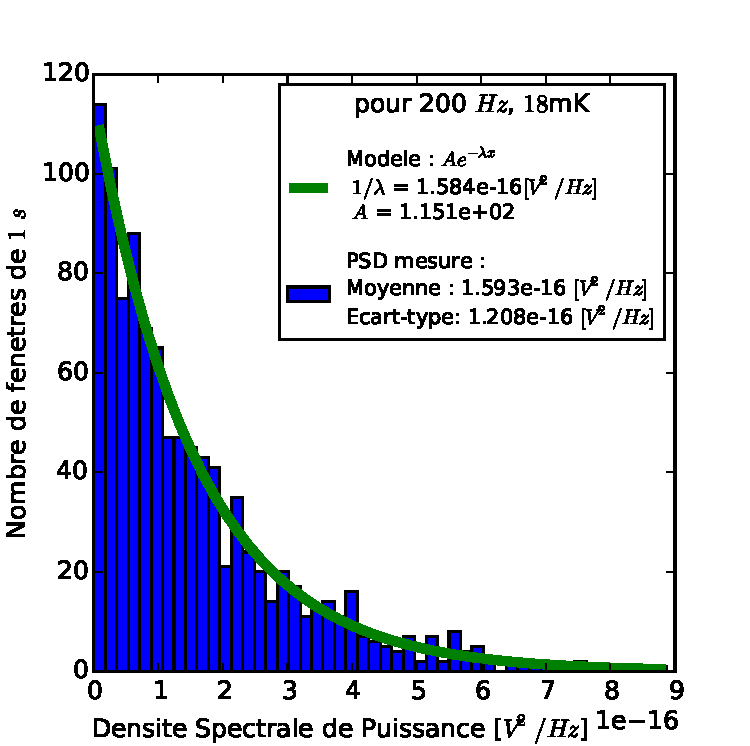
\includegraphics[width=0.6\textwidth]{Images/fit_exp_fin.pdf}
\end{center}
\caption{Histogram of the noise spectral density at $200 Hz$ adjusted by an exponential model.}
\label{noise-form}
\end{figure}

In a first step, the histogram of the measured PSD value for different frequencies is plotted. Such a histogram is presented for a frequency of $200$Hz on the figure \ref{noise-form}. Regardless of the frequency probed, the temperature of the cryostat, or the electronics used, a similar distribution pattern is observed. An exponential distribution is successfully fitted to these histograms. A property of the exponential distribution can be applied to the noise: the mean value $\mathcal{D}_i$ of a measurement at frequency $i$ is equal to its standard deviation $\sigma_{\mathcal{D}_i}$. Indeed, the experimental values of the mean and the standard deviation are close to the term $1/\lambda$.
Thus, on a measure averaged over $N=120$ windows of $1$ second, the Central Limit Theorem expresses the standard deviation on the averaged measure $\sigma_{\bar{\mathcal{D}}_i}$ such that:
\begin{equation}
\label{sigma}
\sigma_{\bar{\mathcal{D}_i}} = \frac{\sigma_{\mathcal{D}_i}}{\sqrt{N}} = \frac{\bar{\mathcal{D}_i}}{\sqrt{120}}
\end{equation}

This information on the PSD of the noise allows to rigorously construct a likelihood function based on the $\chi^2$ function related to the noise model with the parameters $\Theta$ and the experimental data $\mathcal{D}$. It is written as :
\begin{equation}
\label{chi2}
\chi ^2 (\Theta|\mathcal{D}) = \sum^{N_{Temp}}_{j} \sum^{N_{bin}}_{i} \left[ \frac{\bar{\mathcal{D}_{ij}} - \mathcal{M}(f_{ij}; \Theta)}{\sigma_{\bar{\mathcal{D}_{ij}}}} \right]^2
\end{equation}
where we sum over the set of frequencies $N_{bin}$ and over the set of measurement temperatures $N_{Temp}$. In fact, the model is simultaneously adjusted on several PSD measurements carried out for temperatures ranging from $18$mK to $40$mK. We thus hope to obtain better constraints on the parameters, firstly because more points are analyzed, but above all because the change in temperature modifies system parameters (in particular the resistance of the NTD $R(T_e)$) and removes the problems of degeneration between the different free parameters.

Motivated by a Bayesian approach \cite{julian}, the likelihood function is expressed as,
\begin{equation}
\label{likelihood}
\mathcal{L}(\Theta | \mathcal{D}) = \exp{\left(\frac{-\chi ^2 (\Theta|\mathcal{D})}{2}\right)}
\end{equation}

\subsection{Monte Carlo Markov Chain Monte Carlo Analysis (MCMC)}


We look for the set of parameter $\Theta$ that minimizes the likelihood function $\mathcal{L}(\Theta | \mathcal{D})$. To do this, we apply a Markov Chain Monte Carlo analysis called the MCMC method. It is a method based on random walk with condition of one (or more) Markov chain, a set containing the free parameters, in the dimensional space $N=7$ corresponding to the number of free parameters. It has been shown that with a correct likelihood function, the Markov chain allows to sample this function in a neighborhood of the optimal solution . The advantages of the MCMC method are that it can probe a large part of the free parameter space but that it converges quickly to the neighborhood of the optimal solution which can then be explored and analyzed with histograms of Markov chain positions. The figure (\ref{triangle-mcmc}) shows such histograms for EDELWEISS electronics.
\begin{figure}
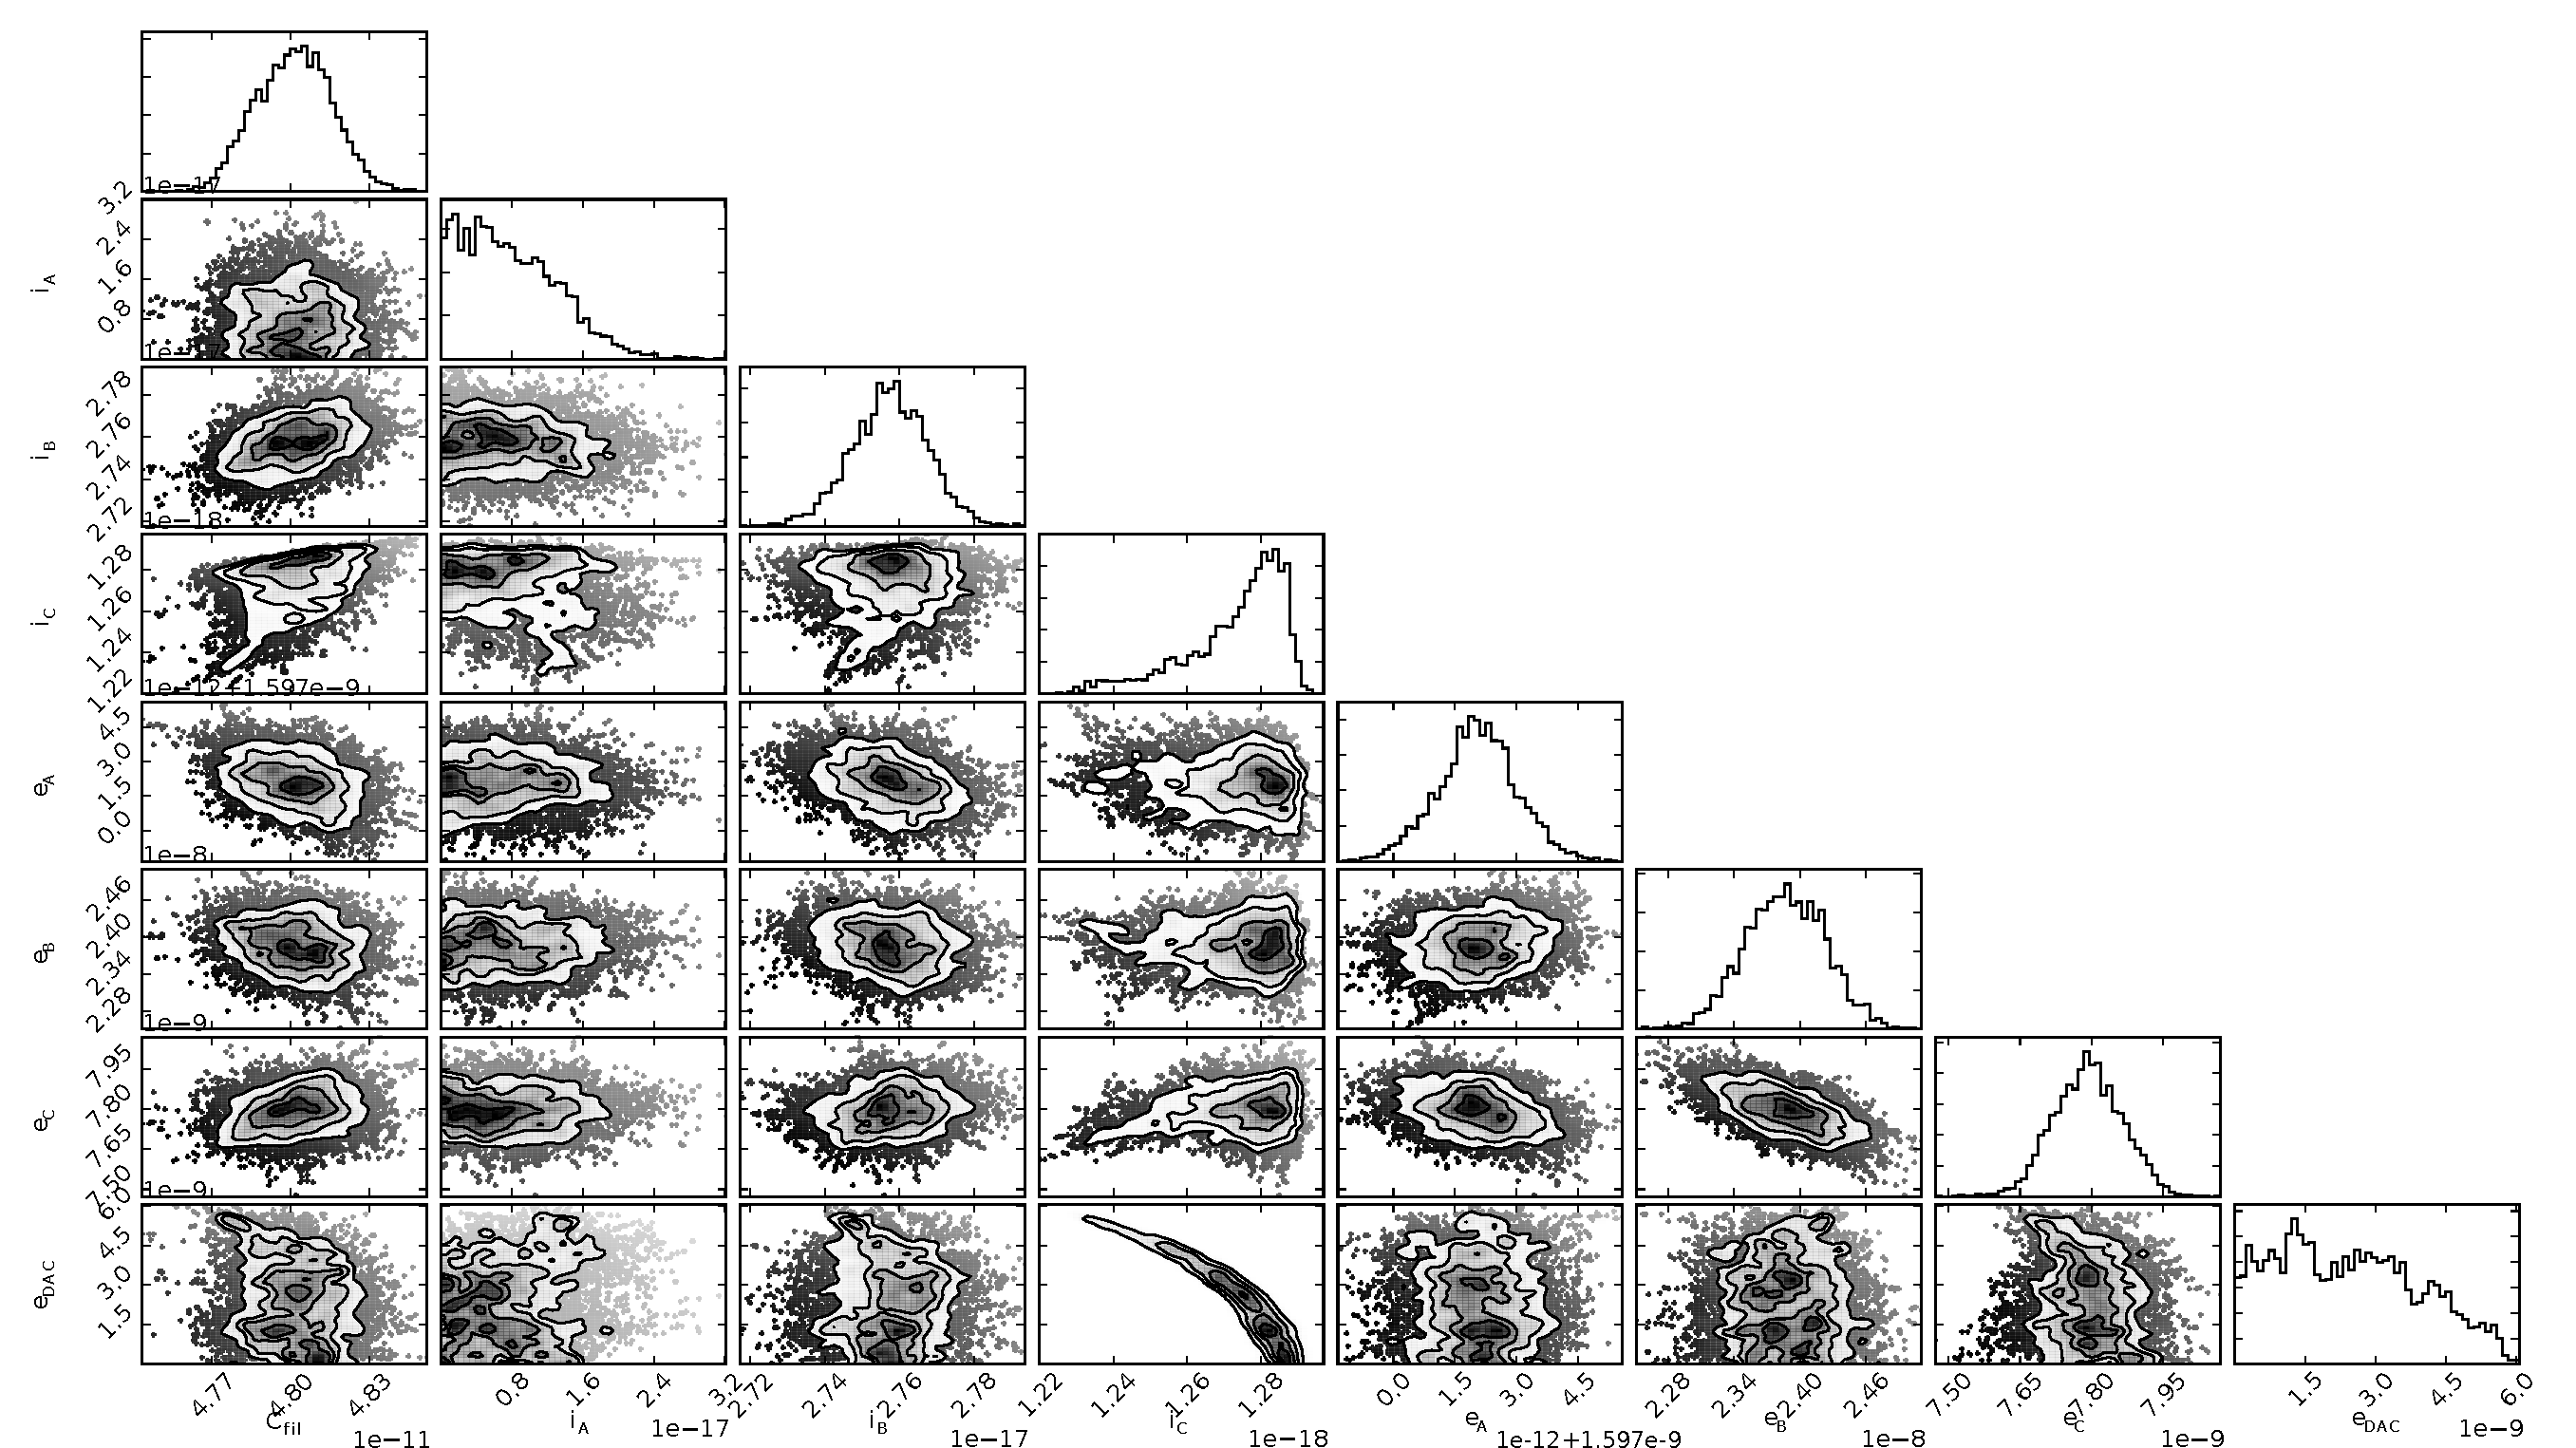
\includegraphics [width=\textwidth]{Images/triangle_fin.pdf}
\caption{Histogram of Markov chain positions with 2-dimensional projections, during MCMC analysis for EDELWEISS electronics. The free parameters presented are from top to bottom, and from left to right: $C_{thread}, i_A, i_B, i_C, e_A, e_B, e_C, e_{DAC}$.}.
\label{triangle-mcmc}
\end{figure}
From the position histogram, the mean position is extracted as an estimate of the set of optimal free parameters as well as the $68\%$ error bars on this estimate from the 16th and 84th quantiles of the distributions. The shape of the distributions also informs us about the quality of the constraint imposed on the considered parameter. Indeed, a narrow distribution indicates a well constrained parameter (parameter $i_B$) with small error bars contrary to a spread distribution which predicts large error bars (parameter $i_A$). Two parameters whose projection in 2 dimensions is elongated indicates their correlation (parameter $i_C$ and $e_{DAC}$). 

\begin{figure}[!ht]
\begin{center}
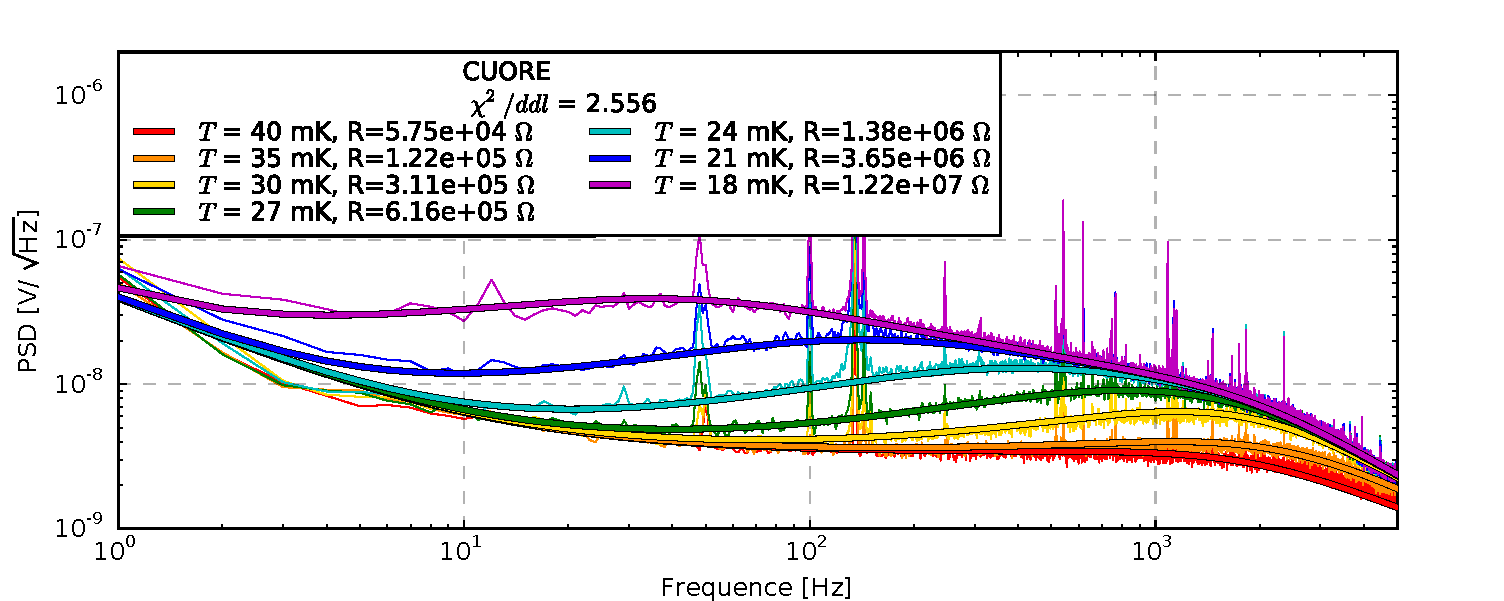
\includegraphics[width=\textwidth]{Images/cuore_fit_fin.pdf}
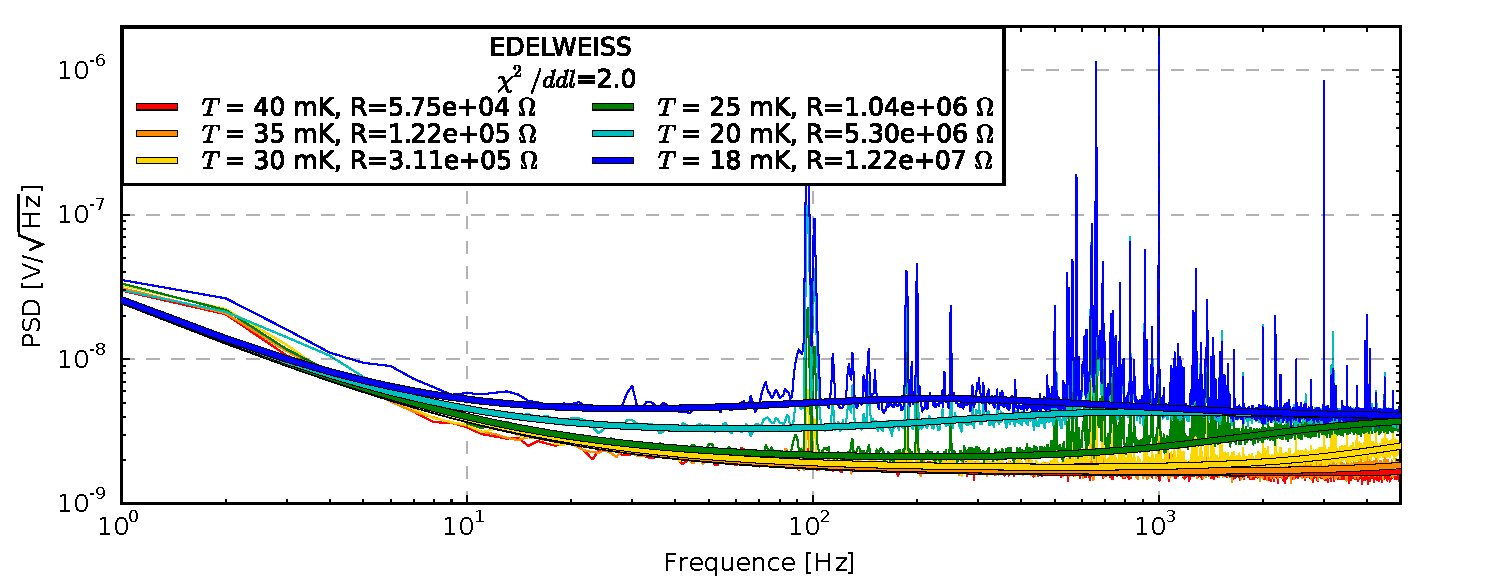
\includegraphics[width=\textwidth]{Images/edel_fit_fin.pdf}
\end{center}
\caption{Averaged measurements (thin lines) and adjustment by MCMC analysis (thick lines) of noise spectral densities for different temperatures on both electronics: CUORE and EDELWEISS. It is important to note that these are noise measurements performed without polarization current. For each cryostat temperature $T$ is specified the value of the thermistor $R$. The term $\chi^2/ddl$ indicates the value of the function $\chi^2$ divided by the number of points (degrees of freedom) of the fit. For a perfect modeling of the experimental data: $\chi^2/ddl \rightarrow 1$}
\label{rainbow-plot}
\end{figure}

After MCMC analysis, we obtain the fit of the experimental data relating to CUORE and EDELWEISS electronics presented in the figure (\ref{rainbow-plot}). The adjustment was performed on the PSD envelope, the parasitic peaks were ignored for the analysis. For the CUORE electronics, a cut-off above $2$kHz is observed: this comes from a low-pass filter integrated in the electronics. It has been taken into account and therefore does not affect the convergence of the MCMC for CUORE. We also note the appearance of two additional free parameters. The $f_B$ parameter corresponds to the order of the low-pass filter for CUORE measurements. The parameter $e_{DAC}$ corresponds to the noise of a power supply connected in series with the capacity of the EDELWEISS electronics. The addition of these additional parameters gives more flexibility to the model so that it better adapts to the experimental data, and thus does not distort the optimal solution.

\begin{align}
\label{result}
\begin{aligned}[c]
& \textrm{\textbf{CUORE}} \\
C_{fil} &= (2.94 \pm 0.01)\times 10^{-10}&[F] \\
i_A &= (1.9 \pm 0.03) \times 10^{-15}&[A/\sqrt{Hz}] \\
i_B &= (6.11 \pm 0.01) \times 10^{-16}&[A/Hz] \\
i_C &= (1.16 \pm 0.01) \times 10^{-17}&[A/Hz^{3/2}] \\
e_A &= (3.28 \pm 0.01) \times 10^{-9} &[V/\sqrt{Hz}] \\
e_B &= (3.03 \pm 0.04) \times 10^{-8}&[V] \\
e_C &= (1.08 \pm 0.02) \times 10^{-8} &[V \cdot \sqrt{Hz}] \\
f_B &= (2.70 \pm 0.01) & [u.a.]
\end{aligned}
\quad \vrule{} \quad
\begin{aligned}[c]
& \textrm{\textbf{EDELWEISS}} \\
C_{fil} &= (4.80 \pm 0.02)\times 10^{-11}&[F] \\
i_A &= (6.17 \pm 4.8) \times 10^{-18}&[A/\sqrt{Hz}] \\
i_B &= (2.76 \pm 0.01) \times 10^{-19}&[A/Hz] \\
i_C &= (1.28 \pm 0.02) \times 10^{-18}&[A/Hz^{3/2}] \\
e_A &= (1.60 \pm 0.00) \times 10^{-9} &[V/\sqrt{Hz}] \\
e_B &= (2.39 \pm 0.04) \times 10^{-8}&[V] \\
e_C &= (7.81 \pm 0.07) \times 10^{-9} &[V \cdot \sqrt{Hz}] \\
e_{DAC} &= (2.02 \pm 1.9) \times 10^{-9}&[V/\sqrt{Hz}] 
\end{aligned}
\end{align}

We check that the fit is excellent on all frequencies, with a certain reserve for the low frequencies of the CUORE electronics. Indeed, the function of $\chi^2$ weighted by the number of degrees of freedom $ddl$ is equal to $2.556$ for CUORE and $2.0$ for EDELWEISS, which is close to the $1$ value corresponding to a perfect modeling. The optimal solutions, indicated in (\ref{result}), for the electronics allow to simulate well the noise of the electronics from the proposed model (\ref{i-ampli}, \ref{e-ampli}). Different behaviors are observed depending on the temperature of the cryostat.  By noting, thanks to the equation (\ref{ode-mat}) and the \ref{block-diagram}, that the contribution of the current noise $i_{noise}$ increases with the complex impedance $Z_{eq}$, we can explain that the PSD levels are higher at low temperature. Indeed, the NTD resistance $R(T_e)$ increases very strongly when the temperature of the cryostat decreases, so the complex impedance $Z_{eq}$ also increases.

The low-frequency behavior of the two electronics is very similar: one observes a strong rise at low frequencies associated with the parameters $e_{B,C}$. At higher frequencies, we note that the electronics of CUORE are much more sensitive to temperature than EDELWEISS. For all temperatures, the noise level of the CUORE electronics is higher than that of EDELWEISS. We simply have a factor of 2 at $40$mK while we have almost an order of magnitude difference at $18$mK. The results \ref{result} show a difference of two orders of magnitude between the current noise $i_A$ of CUORE and that of EDELWEISS. The latter is coupled to the complex impedance $Z_{eq}$ and explains the measured noise level.

\begin{figure}[!ht]
\begin{minipage}{0.49\textwidth}
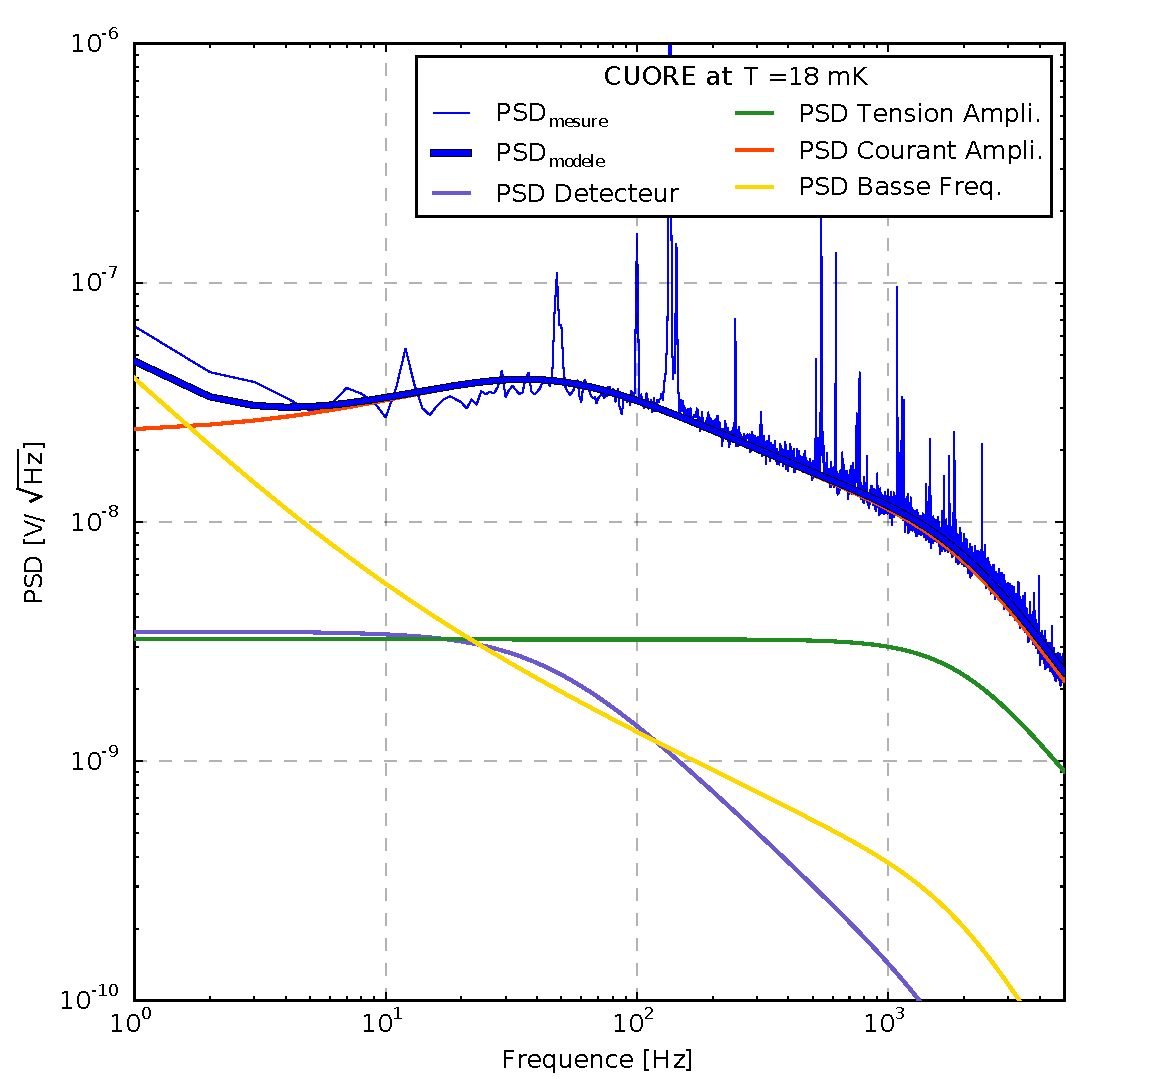
\includegraphics[width=\textwidth]{Images/cuore_18.pdf}
\end{minipage}
\hfill
\begin{minipage}{0.49\textwidth}
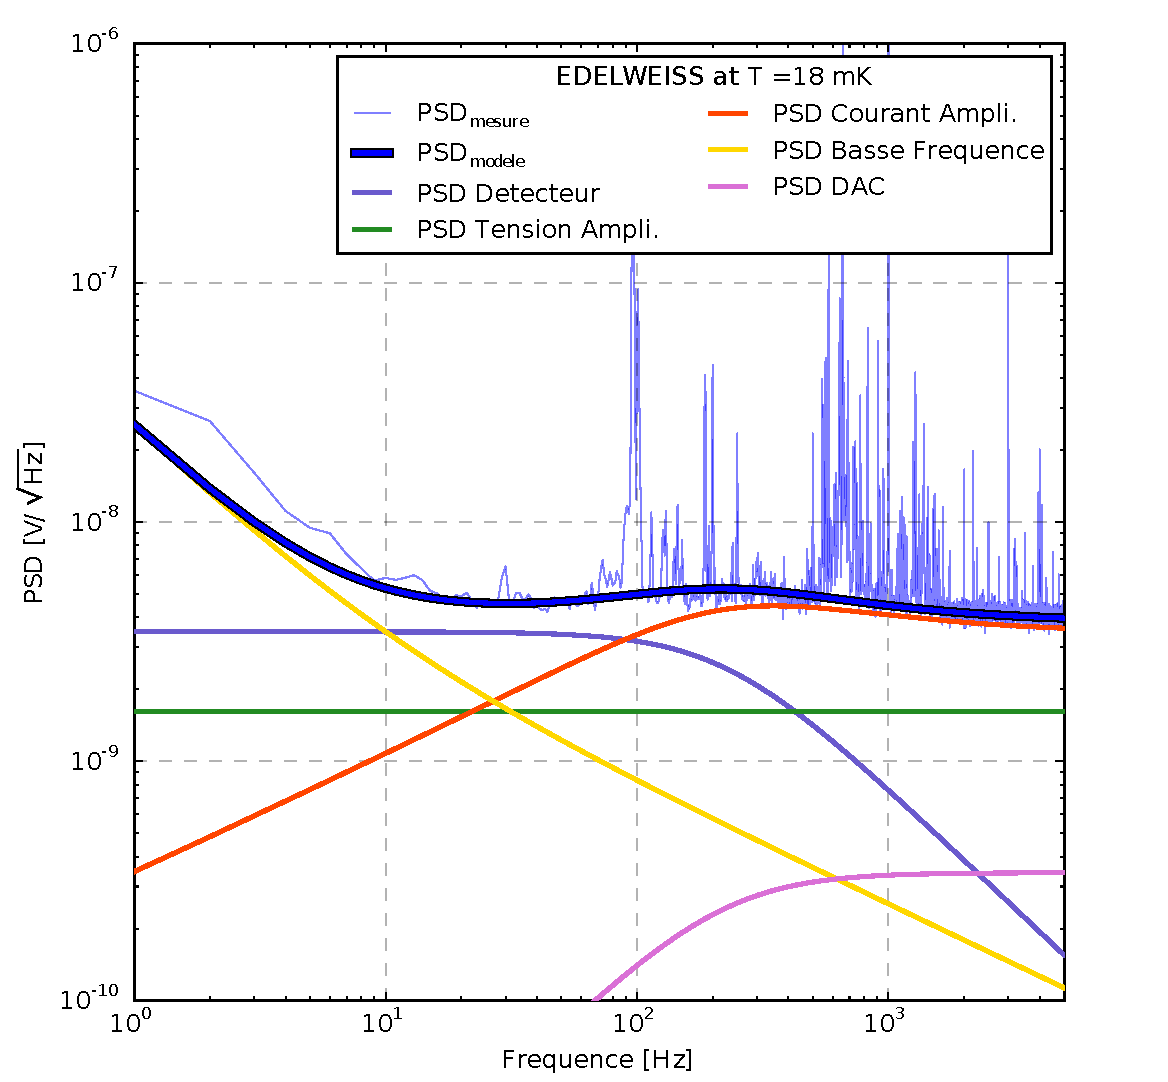
\includegraphics[width=\textwidth]{Images/edel_18.pdf}
\end{minipage}
\caption{Experimental measurement and model of a noise spectral density at $18$ mK for CUORE (left) and EDELWEISS (right) electronics with visualization of the contributions of the different noise sources.}
\label{noise-sources}
\end{figure}

It therefore appears that the least noisy electronics is that of EDELWEISS. It is thus with this electronics that it is agreed to optimize the resolution of the detectors. Nevertheless, the EDELWEISS electronics require certain modifications in order to be used with a non-zero polarization (replace the capacitance by a load resistor). This being at the project stage, only the CUORE electronics can be used for measurements with polarization to characterize the RED10 detector. As it has also been characterized, this does not pose any particular problems.

Using the optimal solution found with the MCMC analysis, it is possible to visualize the contributions of the different noise sources to the total noise PSD, an example at $18$mK is shown in figure \ref{source-noise} for the electronics of CUORE and EDELWEISS. It can be seen that the current noise of CUORE is very high and dominates almost the whole frequency range. The Johnson noise cut-off frequency, which is different for the two electronics, illustrates the influence of the wiring capacity. Indeed, we have $f_{cut} = 2\pi/(R_{NTD} C_{fil})$ considering $R_L\gg R_{NTD}$. A higher cut-off frequency is found in the case of EDELWEISS which has a lower wiring capacity (see \ref{result}). It is also possible to study the predominance of noise sources as a function of frequency. For the electronics of EDELWEISS :
\begin{itemize}
\item below $10$Hz, the noise is dominated by the low-frequency contributions of noise in voltage $e_{B,C}$.
From $10$Hz to $100$Hz, the total noise is based on the intrinsic noise of the detector (TFN noise and Johnson noise of the NTD). This is exactly what is sought: one seeks to be limited by these detector thermal noises which sets the ultimate attainable limit.
\item above $100$Hz, the current noise of the amplification electronics characterized by the coefficients $i_{A,B,C}$ becomes predominant.
\end{itemize} 

\begin{figure}[!ht]
\begin{minipage}{0.49\textwidth}
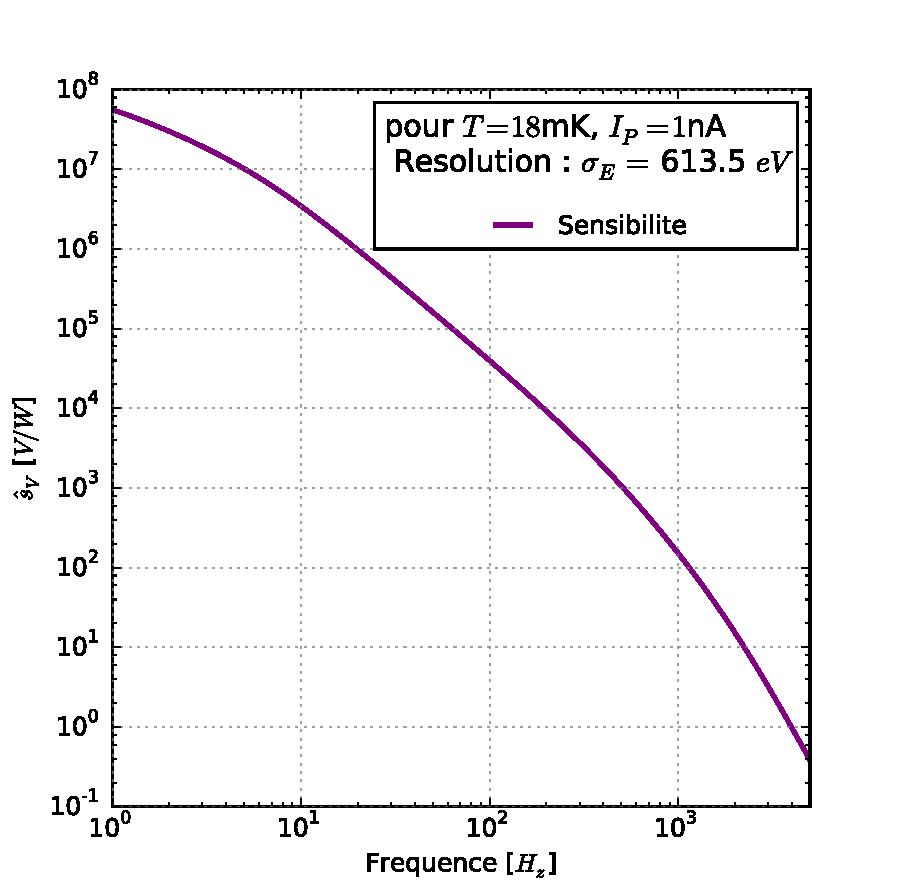
\includegraphics[width=\textwidth]{Images/sv_fin.pdf}
\end{minipage}
\hfill
\begin{minipage}{0.49\textwidth}
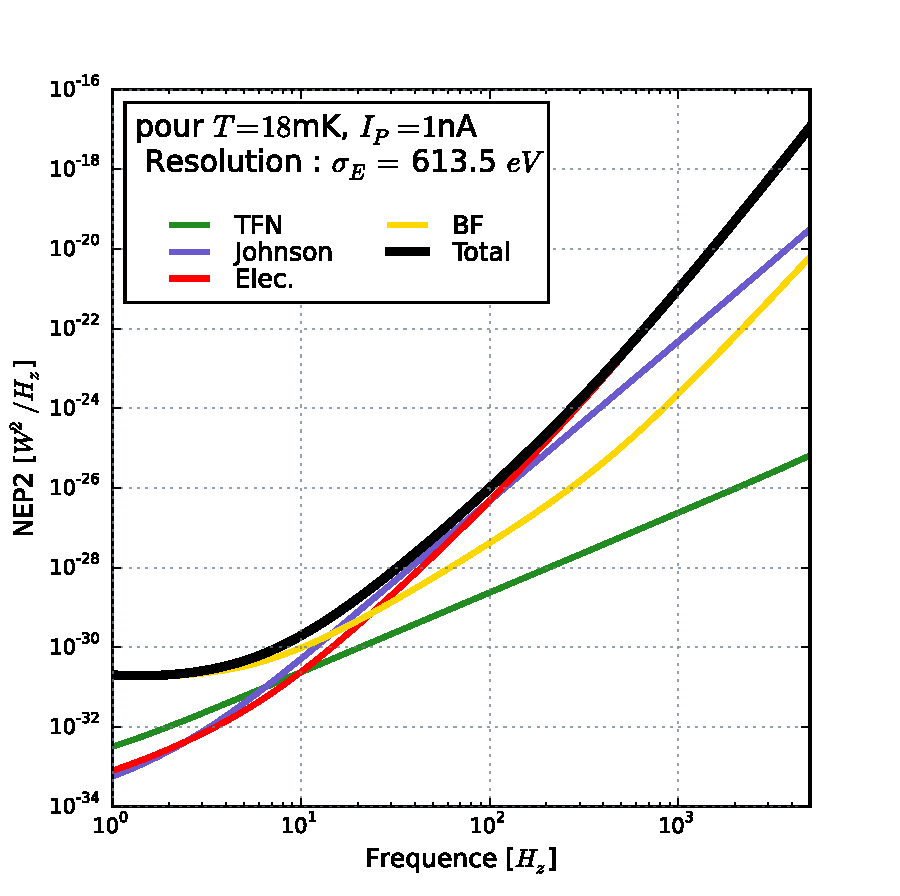
\includegraphics[width=\textwidth]{Images/nep_fin.pdf}
\end{minipage}
\caption{Simulation of sensitivity (left) and CIP (right) with contributions of different noise sources for EDELWEISS electronics at a cryostat temperature of $T=18$mK and a bias current of $1$nA.}
\label{nep-fig}
\end{figure}

\subsection{PEN plotting and resolution calculation}
\label{nep-res}

Now that we have constrained all the parameters of the noise model, it is possible to finalize the computation of the resolution \ref{resolution} with the computation of the NEP \ref{nep}. Figure \ref{nep-fig} shows sensitivity and CIP graphs of the detector with EDELWEISS electronics at $18$mK for a bias current of $1$nA. The sensitivity is consistent with the transfer function of a thermal system: it is indeed a low-pass. Combining according to the formula (\ref{nep}) this sensitivity with the PSD of total noise characterized previously allows to obtain a simulation of the CIP which presents its lowest values between $1$Hz and $100$Hz. 

%\begin{figure}[!ht]
%\begin{center}
%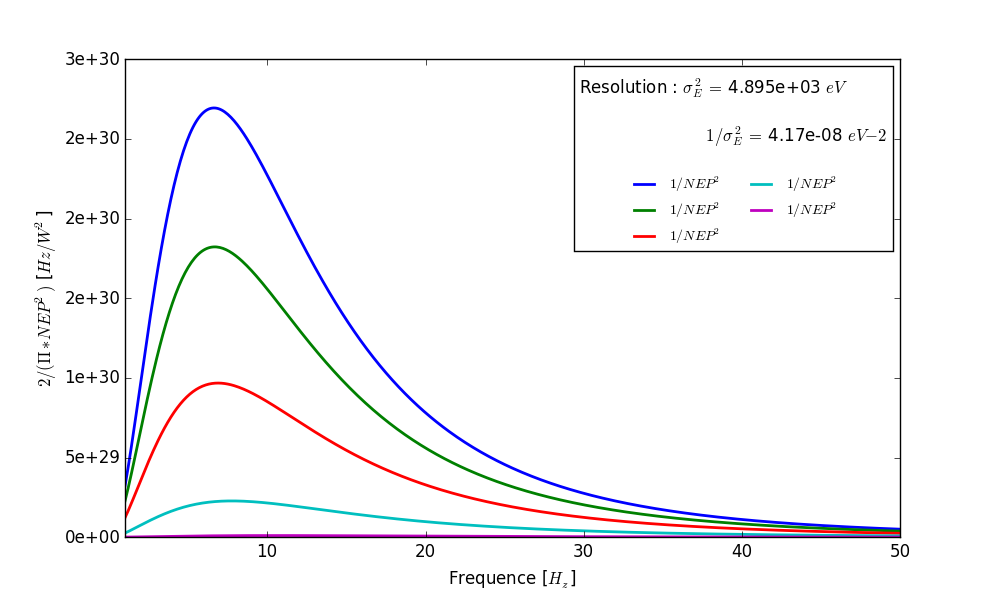
\includegraphics[width=0.7\textwidth]{Images/inte.png}
%\end{center}
%\caption{Simulation de la fonction $\frac{2}{\pi \times NEP^2(\omega)}$ qui apparaît comme intégrande dans la formule de la résolution (\ref{resolution}).}
%\label{inte}
%\end{figure}
It is now possible to access the resolution of this experiment configuration with the formula (\ref{resolution}). We calculate here a resolution of $613.15$eV for EDELWEISS, and a resolution of $1061.7$eV for CUORE, with a temperature of $18$mK and a bias current of $1$nA. A lower value is obtained with the EDELWEISS electronics, which further confirms the choice of this electronics for the optimization of the resolution.

The formula for calculating the resolution (\ref{resolution}) indicates that the lowest CIP values contribute the most to the resolution. Although integrating over a wider frequency range results in lower resolution, the gain becomes negligible as the CIP value increases.
Note that the CIP takes its minimum values around $10$Hz: most of the measurement information is contained in a frequency range from $0$Hz to about $50$Hz. The gain in resolution by integrating beyond $50$Hz is very small. The frequency range of interest for the study of the signal is then identified. By observing the contributions of the different noise sources to the CIP in figure \ref{nep-fig}, we can see that it is low frequency noise that dominates in this frequency range of interest, followed by the Johnson noise of the NTD resistor. We understand that to further decrease the resolution of these detectors, we must work to increase the sensitivity of the system to an event or reduce the low-frequency noise. Part of the Manoir team is already working to understand this low-frequency noise.

\subsection{Thermal characterization of the RED10 detector}

The RED10 detector has only recently come into the possession of the Manor group. Its design is identical to that of RED1. The difference with the latter lies in the type of glue used (glue from the CRESST experiment) and the dimensions of the NTD used. Some thermal parameters are then modified compared to RED1. It is thus necessary to characterize these thermal parameters for a new detector. One will be able to study its response to an event as it was done with RED1 in the previous parts.

\subsection{Current-voltage characteristic and signal shape}

The characterization of the thermal parameters uses the electro-thermal model that was built previously. We will want to adjust the unconstrained parameters to the experimental data with an MCMC analysis as for the characterization of the electronics. This time, the set of free parameters is :
\begin{equation}
\Theta = (R_0, T_0, g_{ep}, g_k, g_{glue}, \epsilon, \tau_P)
\label{theta-red10}
\end{equation}
Indeed, the new glue used has a different conductivity $g_{glue}$. The new geometry of the NTD (and also its slightly different neutron doping) will lead to a modification of the resistance $R_0$ and characteristic temperature $T_0$ present in the equation (\ref{ntd}). The change in dimension also impacts the electron-phonon coupling $g_{ep}$ and the Kapitza conduction coefficient $g_k$. A priori, the volumetric thermal capacities of the absorber and the NTD remain unchanged, which makes it possible to recalculate the new thermal capacities from the known dimensions of the NTD. It would have been possible to include these in the free parameters, but the choice to fix them was favored in order to avoid degeneration problems and thus better constrain the parameters.
A preliminary study of the signal shape (shown on the right of figure \ref{v2i-red10}) of RED10 revealed that the pulse decay has two characteristic time constants. This type of signal has never been observed on signal measurements performed with RED1: there is only one characteristic decay time explained by the thermal leakage to the cryostat from the electron bath with a recoil energy deposit in the absorber. The presence of a second characteristic time for RED10 can only be explained by the presence of athermic phonons as introduced in section \ref{omega}. These are phonons that do not immediately relax in the absorber, but pass through the NTD sensor before relaxing. They thus create a temperature rise directly within the NTD. The source term $\bm{F}$ in the equation (\ref{ode-mat}) is then rewritten:
\begin{equation}
\bm{F}(t-t_0) = 
\left( \begin{array}{c}
(1-\epsilon)E/C_a \
0 \\
\epsilon E/C_e \\\
0
\end{array} \right) \delta (t-t0)
\end{equation}
with $\epsilon$ the fraction of recoil energy converted into athermic phonons. The normalization constants of the general time solution (\ref{eigein-solc-expr}) depend on the source term $\bm{F}$ according to (\ref{normal}) and therefore differ from the case of RED1 without athermal phonons. This has the effect of better expressing a new exponential, and thus a new characteristic time, contained in the general solution. This observation of two characteristic times for the signal motivates the addition of the fraction of athermic phonons $\epsilon$ and their characteristic relaxation time $\tau_P$ to the free parameters of the model.

The current-voltage characteristics and the shape of the signal at an event of the natural radioactivity with a fixed bias current $I_P=4$nA are measured on RED10 for different temperatures ranging from $18$mK to $30$mK. Thus, we study the behavior of RED10 in the steady state (section \ref{steady-section}) and in the time regime (section \ref{temporal}).
The likelihood function analysis is performed with the MCMC method as in section \ref{caract}. Experimental data with the fitted models are presented in the figure (\ref{v2i-red10}).

\begin{figure}[!ht]
\begin{minipage}{0.49\textwidth}
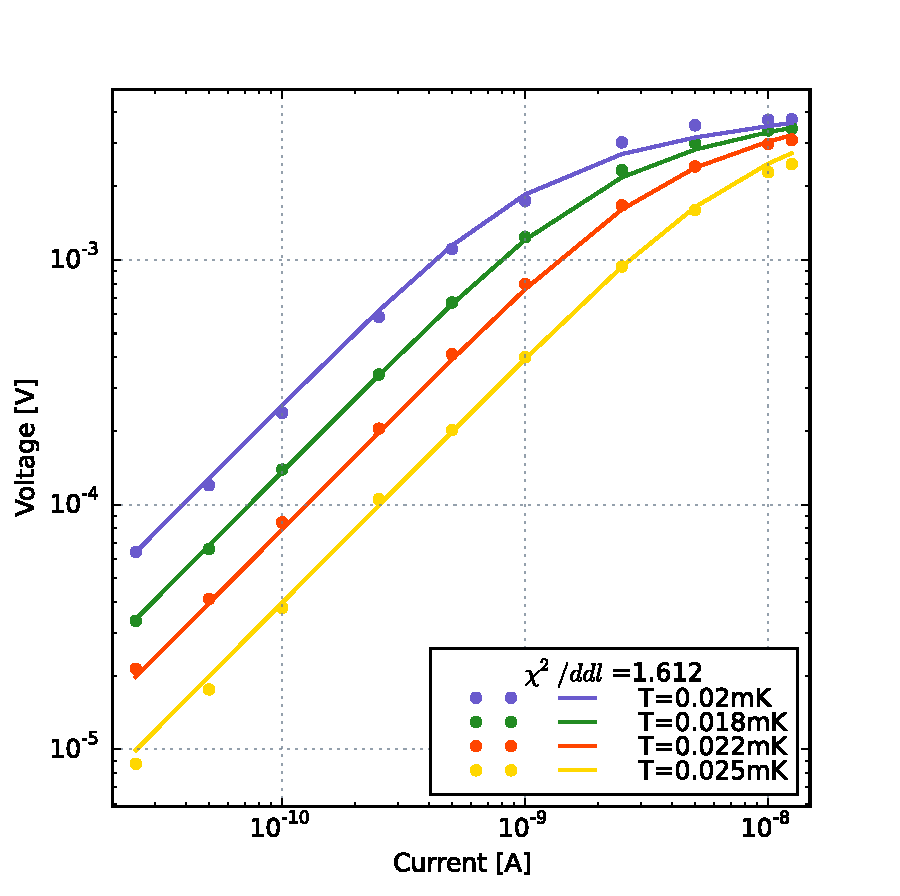
\includegraphics[width=\textwidth]{Images/v2i_red10.pdf}
\end{minipage}
\hfill
\begin{minipage}{0.49\textwidth}
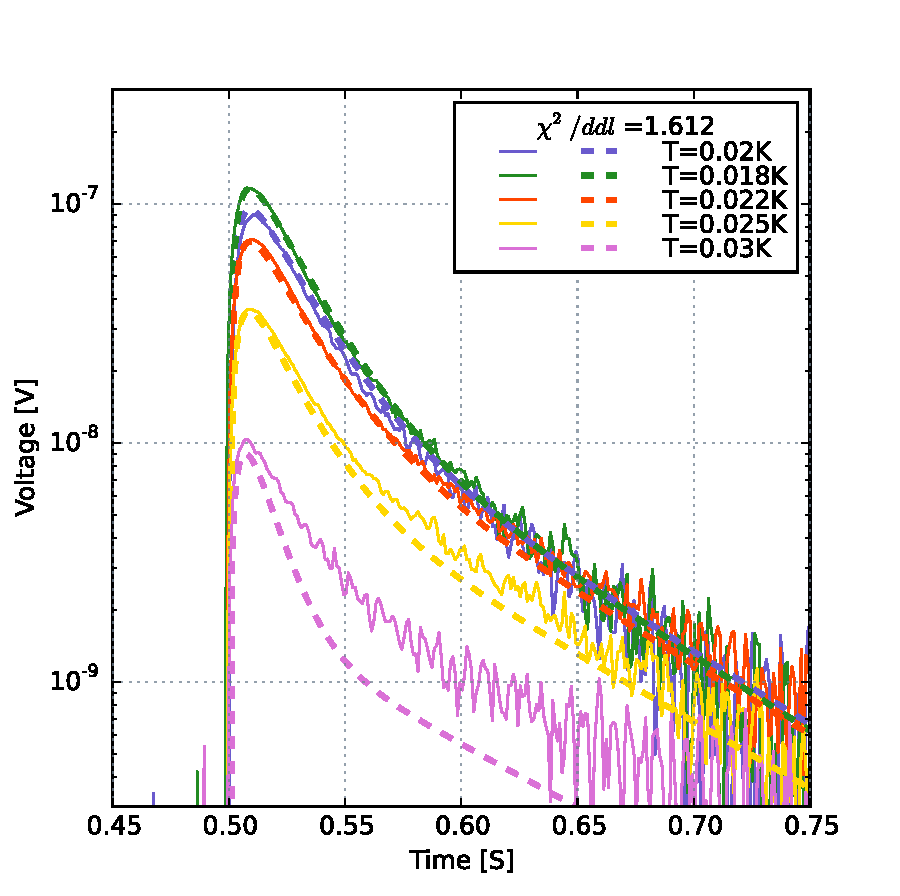
\includegraphics[width=\textwidth]{Images/pulse_red10.pdf}
\end{minipage}
\caption{Experimental measurement and model fitting of the current-voltage characteristic (left) and a signal created by an ambient radioactivity event (right) for the RED10 detector.}
\label{v2i-red10}
\end{figure}

The fit seems good for both types of measurement with $\chi^2/ddl=1,612$. However, there is a difficulty in adjusting the pulse for a temperature of $30$mK. The current-voltage characteristic makes it possible to constrain the free parameters involved in the steady state equations: $R_0, T_0, g_{ep}, g_k$. The analysis of these equations (\ref{steady}) gives us that the linear part of the characteristic constrains mainly the resistance value of the NTD, and thus $R_0, T_0$. The voltage plateau at higher bias current comes from an excessive Joule effect which is then no longer compensated by the thermal leakage to the cryostat. The NTD then increases in temperature, losing electrical resistance with a constant bias current, which causes the voltage plateau to appear. Its adjustment thus constrains the values of conductivity $g_k$ and electron-phonon coupling $g_{ep}$.

As for the shape of the signal, the model shows two slopes and thus two characteristic times. The adjustment of these two decay slopes constrains the athermic phonon fraction $\epsilon$, and more generally, all the parameters involved in the calculation of the normalization constants of the eigen-base of the solutions (\ref{eigen-soluc}).
The rise in tension allows to constrain the relaxation time of the phonons $\tau_P$. Indeed, for an immediate relaxation of the phonons, the rise time would be infinitely large (modulo the cutoff frequency $(RC_{fil})^{-1]}$).

The MCMC method then gives the following constraints for RED10:

\begin{align}
R_0 &= (11.6 \pm 0.4)&[\Omega] \\
T_0 &= (2.72 \pm 0.01) &[K] \\
g_{ep} &= (21.1 \pm 4.4) &[W/K^6/cm^3] \\
g_k &= (2.77 \pm 0.1) \times 10^{-4}&[W/K^4/mm^2] \\
g_{glue} &= (7.46 \pm 1.67) \times 10^{-4} &[W/K^{n_g}/mm^2] \\
\epsilon &= (0.202 \pm 0.001)  & [fraction]\\
\tau_P &= (4.03 \pm 0.03) \times 10^{-3} &[s]
\end{align}


These thermal parameter values are of the same order of magnitude as those corresponding to RED1. It is important to highlight the high portion of athermal phonons of about $20\%$ which is to be compared to their complete absence with the RED1 detector. This is a new observation for this type of detector. Their high presence results in an acceleration of the voltage signal and thus an increase of the frequency range of interest of the signal introduced in the section \ref{nep-res}. In addition, athermic phonons are not affected by the capacity of the absorber, and transmit all their energy directly to the NTD. Understanding and increasing the rate of athermal phonons will thus allow the resolution of the detector to be lowered. A new way of optimizing the detectors has been discovered, which is not yet considered within the EDELWEISS collaboration.

\subsection{Red10 noise and resolution}

Since RED10 is fully characterized from the thermal point of view, and the CUORE electronics used for the measurements are also characterized, we are able to simulate the noise spectrum related to RED10 compared to the experimental measurement. Figure (\ref{noise-red10}) shows the modeling and experimental measurement of the PSD of RED10 noise at a bias current of $4$nA for a temperature of $22$mK. Note that a Bessel filter is applied to the measurement, and to the model, which explains the cutoff appearing from $2$kHz.

\begin{figure}[!ht]
\begin{center}
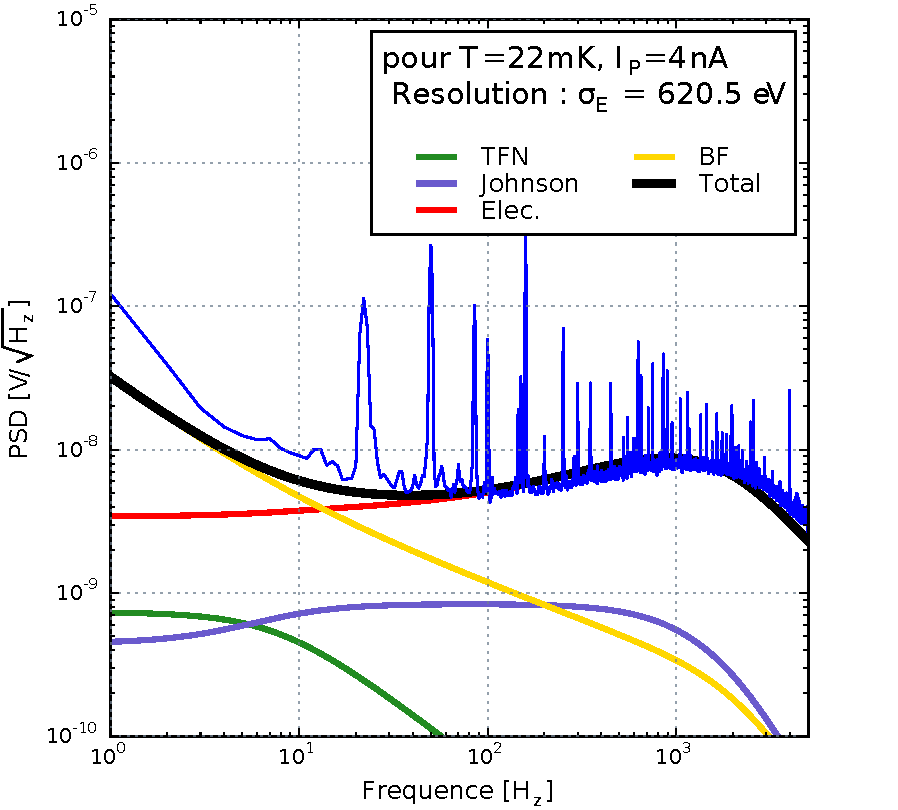
\includegraphics[width=0.55\textwidth]{Images/modexp.pdf}
\end{center}
\caption{Experimental measurement of a spectral density at $22 mK$ with RED10 compared to a simulation of the built model.}
\label{noise-red10}
\end{figure}

The model and the measurement describe very similar developments. We do find the presence of high low frequency noise that dominates up to $15$Hz. It is then the current noise that predominates over the rest of the frequency range. It should be noted that a measurement of noise with bias current is performed here, so it would be incorrect to compare the presented current noise of RED10 with the current noise of RED1 obtained without bias current. However, there is a slight shift in the model from the experimental data to the low frequencies. This can be explained by the underestimation of the low-frequency noise already observed for CUORE electronics in the figure (\ref{rainbow-plot}). The excess of low-frequency noise also comes from the high rate of muon events during the measurements: despite the cuts made in the analysis, part of the signal decay is always recovered, which helps to amplify the low frequencies of the measured spectrum.

The experimental resolution measurement is carried out from the noise PSD and the measurement of a signal. Indeed, renormalizing the amplitude of the signal and applying a Welch method allows to estimate the signal sensitivity of the RED10 detector. The renormalization also requires to know the conversion between the energy deposited in the absorber by an event and the amplitude of the measured signal. This calibration is performed using the interaction of cosmic muons with the absorber. The energy they deposit in the absorber is equal to $18$MeV. Measuring the voltage amplitude of a muon signal therefore allows to deduce the conversion factor necessary for the renormalization of a signal. The application of the discrete analogue of the formula (\ref{resolution}) to a noise spectrum and the previously calculated sensitivity allows the evaluation of an experimental resolution. 

\begin{figure}[!ht]
\begin{center}
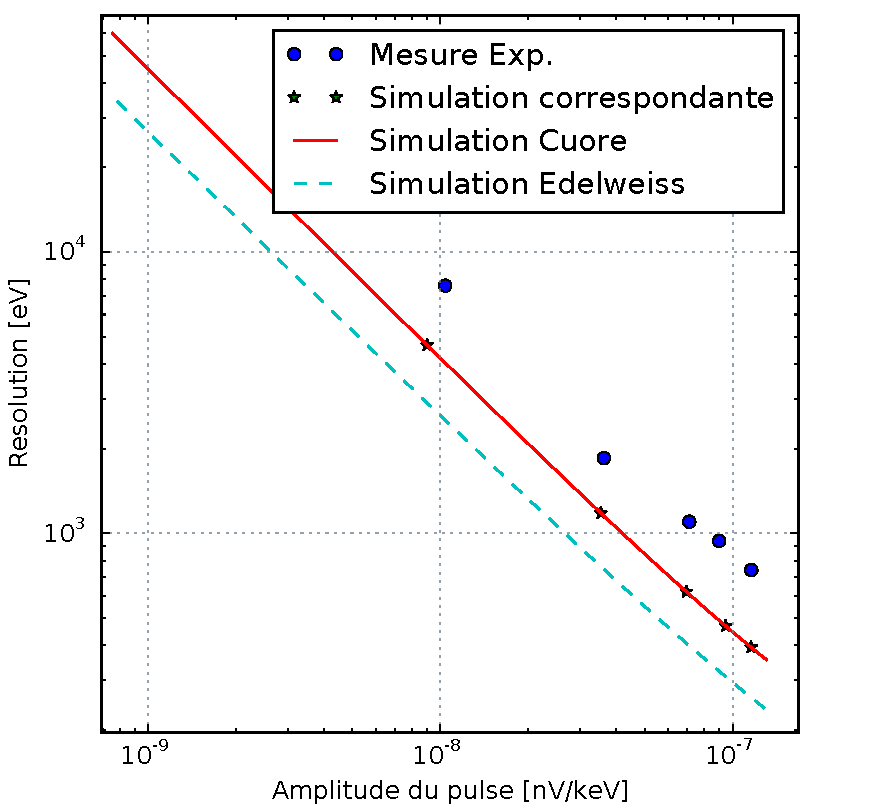
\includegraphics[width=0.55\textwidth]{Images/resamp_fin_fin.pdf}
\end{center}
\caption{Resolution-Signal amplitude characteristic for the RED10 detector for a bias current of $4$nA with temperatures ranging from $18$mK to $30$mK.}
\label{amp-res-red10}
\end{figure}


The figure (\ref{amp-res-red10}) shows the resolutions as a function of the signal amplitude for different temperatures at a fixed bias current. The experimental resolutions are higher than the simulated resolutions. This is explained by the deviation between model and noise measurement observed in figure (\ref{noise-red10}): the modeled low-frequency noise is lower than in reality, hence the prediction of lower resolutions. The pulse amplitude is used to estimate the sensitivity of RED10 to the signal. Except for the $30$mK measurement where the signal was already poorly modeled, the simulated and real amplitude values are almost identical. Moreover, since the two sets of dots show a very similar evolution of the resolution as a function of amplitude, it is deduced that the model is in good adequacy with the experimental reality. A study of the noise difference is still necessary to obtain a complete adequacy of model and experiment.

It should be noted that the measurements were performed with CUORE electronics. The simulation of the resolution-amplitude characteristic is plotted for both CUORE and EDELWEISS electronics. It should be noted that the latter makes it possible to gain almost a factor of 2 on the value of the resolution (the amplitude remains unchanged). This is consistent with the low noise level of EDELWEISS compared to that of CUORE.

\subsection{Optimization of the RED10 detector and perspectives}

An electro-thermal model was built and tested with RED10. Even if some parameters need to be further refined to have a better fit, we can perform a preliminary optimization of the RED10 detector. A simulation of the resolution of RED10 as a function of the bias current flowing through its NTD for different cryostat temperatures is presented in figure \ref{optim}. The simulation is performed with the EDELWEISS electronics which has the lowest noise level, and the temperature of the load resistor is lowered to the temperature of the mixing chamber to reduce its Johnson noise (which will be realized in the next few months).

It is observed that there is an optimum current corresponding to each temperature to minimize the resolution. Indeed, if the NTD thermistor is polarized too much, the heat produced by Joule effect can no longer be evacuated efficiently by the thermal leakage. The temperature of the NTD becomes high and therefore its value drops, which affects the sensitivity of the system. The same effect is observed when plotting the current-voltage characteristic in figure \ref{v2i-red10}. At too low a current, the NTD sensor is no longer polarized enough to efficiently convert the heat signal into a voltage signal: the sensitivity drops as well. No matter what bias current is used, the lowest resolution is always obtained at the lowest temperature. The NTD's resistance formula (\ref{ntd}) explains why the signal is more sensitive at low temperatures: the derivative of the resistance with respect to the temperature takes its maximum values there (in absolute terms). Moreover, lowering the temperature reduces all TFN noise, and the Johnson noise of the NTD thermistor, which further improves the resolution.

\begin{figure}[!ht]
\begin{minipage}{0.49\textwidth}
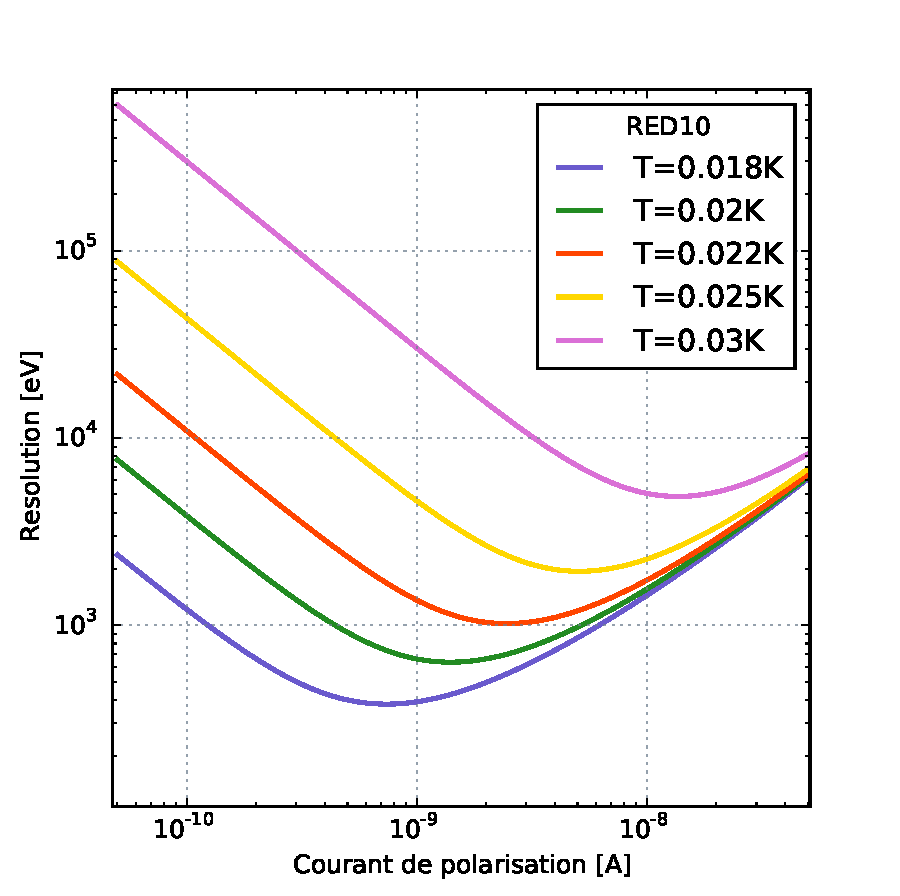
\includegraphics[width=\textwidth]{Images/red10_i.pdf}
\end{minipage}
\hfill
\begin{minipage}{0.49\textwidth}
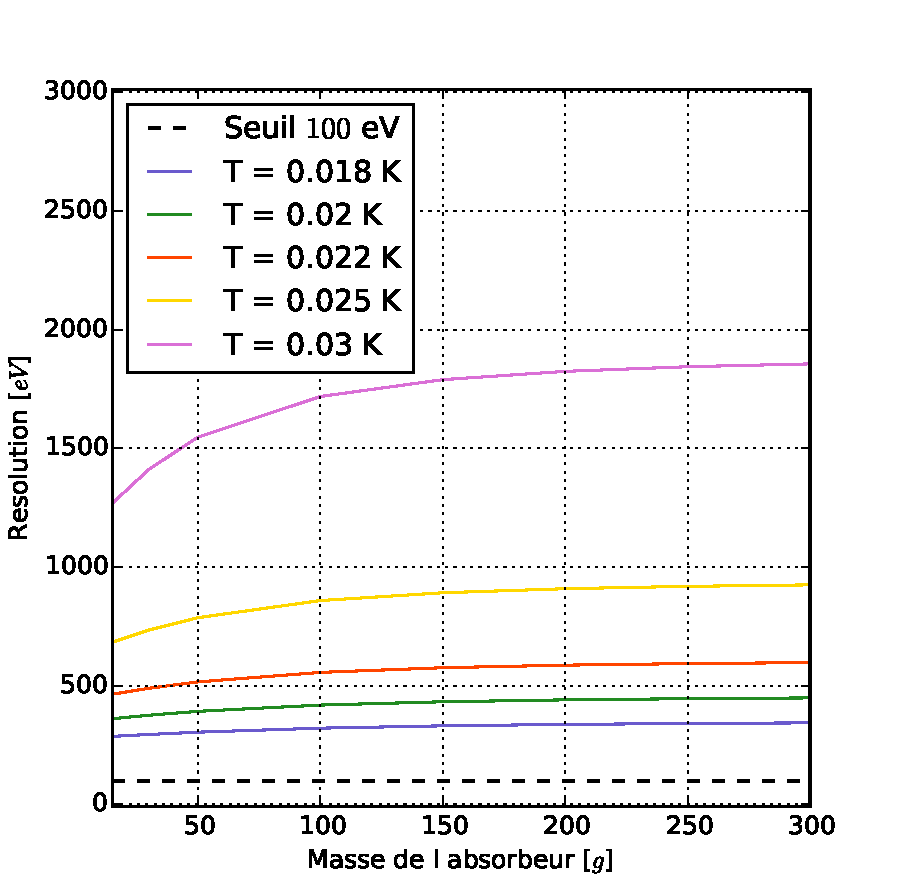
\includegraphics[width=\textwidth]{Images/red10_mass.pdf}
\end{minipage}
\caption{(left) Simulation of the resolution of RED10 as a function of the bias current for different temperatures. \\ (right) Simulation of the resolution with optimized bias current as a function of the absorber mass for different temperatures. The design considered is the same as that of RED10, only the mass of the absorber is changed by adjusting the bias current to obtain the lowest resolution.}
\label{optim}
\end{figure}

The RED10 study was fully realized for a bias current of $4$nA, which corresponds to the optimal current at a temperature of about $24$mK. It would therefore have been possible to obtain better resolution values by adjusting the bias current for each temperature. Thus, it will be important, in the future, to properly determine the optimum polarization current of a detector according to the measurement conditions.

The search for light dark matter requires the development of a new generation of detector with very low detection threshold. For this, it is necessary to work on the design of the detectors. For example, it is necessary to study the behavior of the detector according to the geometry of the NTD, the mass of the absorber or the location of thermal leaks. A simulation of the resolution of a detector as a function of the absorber mass is shown in the graph on the right side of figure \ref{optim}. Note that the polarization current is adjusted for each point to draw an already optimized resolution curve. According to the formula (\ref{capa}), it would be interesting to reduce the thermal capacity of the absorber $C$, by lowering its mass, in order to cause a greater temperature rise $\Delta T$, and thus amplify the heat signal. According to the simulation, this amplification of the heat signal would appear only for very small detector masses, and would remain very modest for low temperatures. 

It is now understood that we remain limited for the moment by another aspect of the detector. In the future, the optimization of the detector will involve the study of the behavior as a function of the dimensions of the NTD thermistor and the thermal conduction surfaces. It already appears that it would be necessary to reduce the thermal capacities of the different baths while maximizing the thermal bonds. 



% Ionization Theory
%% Chapter Electrodes

\chapter{Electrodes Design with Electrostatic Simulation} % Main chapter title

\label{ChapterElectrodes} % Change X to a consecutive number; for referencing this chapter elsewhere, use \ref{ChapterX}

%----------------------------------------------------------------------------------------
%	BEGING CHAPTER
%----------------------------------------------------------------------------------------

Let me tell you about my work with an electrostatic simulation software called COMSOL.
That was quite nice. Just designing the detector and the aluminium electrodes with a beautiful and efficient interface.
Thanks to that, I could simulate a lot of configuration and geometry to probe for the finest results out there.
Finest meaning a lot of fiducial volume, good charge collection, and low electric capacity.
A usual impossible to solve problem which lead to a lot of trade-off in itself, without adding the issues about the heat channel.
But hey, I could obtain some nice plots and tables, check them out.


\section{Electrodes as Sensors for the Ionization Channel}

\subsection{Basics of the Ionization channel}

The ionization channels aims at converting the ionization of the germanium into a voltage signal.
This is done with the use of aluminium electrodes acting as the terminals of a capacitor of capacitance $C$. When collecting an electric charge $\Delta Q$, a voltage $\Delta U$ is created across the capacitor such as:

\begin{equation}
C = Q \times U \quad \Leftrightarrow \quad U \times = \frac{C}{Q}
\label{eq:capacitor-basic}
\end{equation}

A high sensitivity of the ionization channel means that the created voltage $\Delta V$ is maximized. The equation \label{eq:capacitor-basic} shows that a low capacitance $C$ of the electrodes and a high collection of electric charge $\Delta Q$ increase the ionization channel response. While the amount of electric charge $\Delta Q$ can depend of the electric field shape, in the case of a theoretically perfect charge collection, the number of electron-hole pairs created and collected only depends on the recoil energy $E_R$ of the interacting particle $i$ and the associated quenching factor $Q^i(E_R)$. This factor depends only on the material used as absorber, in our case Germanium.
The capacitance depends on the design of the detector, and is the one of the main quantities used to quantify the performance of a detector design.


\subsection{Germanium as Semiconductor}

The material used as absorber for the detectors is semi-conducting High Purity Germanium [ref?].
This paragraph focuses on its characteristics and also compares it to materials used by others experiments using bolometers.

The use of semi-conducting Germanium as an absorber was first proposed by Taverdale? and Evvan [80, Emeline].
Along with an increase in temperature, a semi-conducting germanium also features a phenomenon of ionization caused by a particle interaction. Such electronic and nuclear recoils form electron-hole pairs of average energy $\epsilon = 3 eV/pair$. This energy corresponds to the gap energy separating the valence and conduction electronic bands in the germanium in its semi-conducting state accessible for temperature below 77K.

In order to understand the physical properties of a semi-conductor, we can consider the theory of energy bands. In a solid material, at rest electrons are occupying the lowest state of energy according to their fermion nature. This lowest state of energy are strongly linked to the nucleus, forming the valence electronic band of energy. Higher energy states are able to interact with neighboring atoms and compose the conduction electronic band of energy.
conducting, not conducting, semi-conductor. Small gap. blablabla

The semi-conducting properties of a germanium crystal heavily depends on the impurities affecting it. With the Germanium element being of valence 4, there exist two kind of impurities:
\begin{itemize}
	\item acceptor impurities of valence 3 producing a p-type germanium,
	\item donor impurities of valence 5 producing an n-type germanium.
\end{itemize}
These impurities creates intermediary energy steps in the semi-conducting germanium band gap accessible to electric charges (as seen in figure \ref{fig:conduction-bands}). The presence if this intermediate accessible energy bands has several consequences on the ionization channel. It reduces the energy necessary to create an electron-hole pair, thus creating additional noise and biasing for the ionization channel. Then, it creates a trapping phenomenon which prevent electric charge carriers from reaching the electrodes. With trapped charges in the crystal, a counter electric field slowly generates, reducing the sensitivity of the electrodes. Finally, these impurities lower the global resistivity of the germanium crystal and increase the leakage current.
The semi-conducting germanium use as absorber thus should contain the lowest amount of impurities in order to have a detector with good performances.
The study of the trapping in EDELWEISS detector and the impact of impurities is presenting in [ref quentin 80].
We define $N_a$ and $N_d$ as the number of acceptor and donor impurities respectively. We  can have access (how?) to the absolute difference of this quantities $|N_a - N_d|$ which determine the number of available charge carriers.
The material used as absorber is High-Purity Germanium (HPGe) with an estimated:
$$ 10^{9} < |N_a - N_d| < 10^{10} \textsf{cm}^{-3}$$
which corresponds to less than one impurity atom for $10^{12}$ germanium atoms. With this material, low leakage currents of few pA can be achieved for the usual operating  electric field range of a few V/cm.

Ok, so here might be some mumbo jumbo concerning the p-n junction in a semi-conductor. Is it useful ? idk.
A recurring term is "depletion depth" which apparently is inversely proportional to the impurity concentration.
A germanium crystal with good performance should present a high resistivity obtainable with a high depletion depth.
As a result, the EDELWEISS and RICOCHET experiment use high purity germanium (HPGe) with special treatment [ref?] leading to a low impurity concentration of less than $10^{10}$ atoms.cm${-3}$ (1 impurity for $10^{12}$ germanium atoms) whereas a normal germanium crystal possesses a concentration of about $10^{13}$ atoms.cm${-3}$.

Comparing the germanium to silicium:
\begin{itemize}
	\item higher Z, so better quenching factor [lindhard]
	\item denser material, better for exposure
	\item low impurities, big depletion region
	\item low ionization energy (gap?)
	\item high conductivity (?)
\end{itemize}

\begin{figure}
\centering
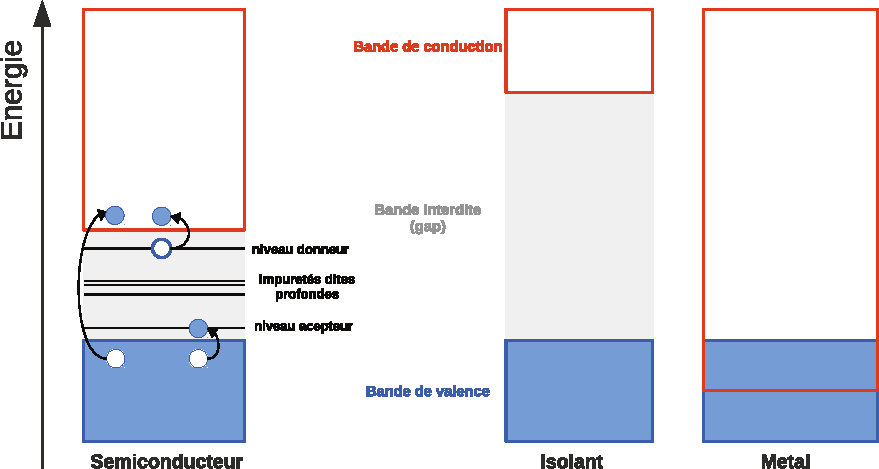
\includegraphics[width=\linewidth]{Figures/Electrodes/conduction_bands.pdf}
\caption{Scheme of the conduction bands for semiconductor, insulator and conductor materials.}
\label{fig:conduction-bands}
\end{figure}


\subsection{Electric Charge Drifting in Crystal}

{\color{red}
Alex B. biblio here.
Also explainin trapping, charge collection.
}

The study of charge migration in EDELWEISS germanium crystal is presentend in [ref Emeline 82] taking into account the crystallographic structure of the germanium crystal. In this study, Alex.B simulates numerically the drifting of eletrons and holes in a 200g FID Edelweiss detector with bulk interaction of gamma-rays of energy 348keV. The charge trajectories are presented in the figure \ref{fig:charge-drifting}. He also follows the generation of the voltage signal on the electrodes. This is consistent with Ramo field theory which will be described later.

When interacting with the atoms of a germanium crystal, a particle deposits a so-called recoil energy. The word "recoil" references to the elastic diffusion of the incoming particle on a germanium nuclei, this is a nuclear recoil, or the elastic diffusion of the electronic cloud of a germanium atom, this is an electronic recoil. A fraction of the recoil energy is used for the creation of electron-hole pairs, this process is known as ionization. This fraction is called quenching factor $Q$ whose value depends on the recoil type, the incoming particle, and the recoil energy. When a electron-hole pair is created, a valence electron is going into the conducting band of the semi-conducting germanium crystal (as illustrated in the figure \ref{fig:conduction-bands}) while a hole appears in the valence band. Following a recoil, electrons can excited with energies much greater than the germanium gap energy. However, such electrons relaxes by phonon emission and creation of new electon-hole pairs. We can consider that after relaxation, the number of electron-hole pairs $N^j$ induced by a recoil of type $j \in {e(lectronic), n(uclear)}$ is expressed as:
\begin{equation}
\label{eq:number-pairs}
N^j = Q^j \left( E_R \right) \frac{E_R}{\epsilon}
\end{equation}
with $\epsilon$ the average energy necessary for the formation of an electron-hole pair and $Q^j$ the quenching factor function of $E_R$ the recoil energy.

The average energy $\epsilon$ contained in a pair is greated than the germanium gap band of $0.67\textsf{eV}$ as it also take into account the momentum associated to the interaction between the pair and the crystal. The figure \ref{fig:band-structure} represents the lower energy of the valence band and the higher energy of the conduction band in a germanium crystal depending on the orientation (orientation of what ? germanium crystallography, electron momentum ?). While the absolute lowest energy of the conducting band, at [111] and the highest energy of the valence band, at [000], are separated by the germanium gap energy of $0.67\textsf{eV}$, this extremum does not correspond to the same orientation $\bm{k}$, the germanium gap is indirect. An electron can transition into the conducting band with the transfer of a momentum $\bm{k}$ from the phonon in order to respect the conservation of momentum and energy (as described in [ref quentin 87]). In the end, the average energy of a pair in germanium is estimated to [ref necessary]:
\begin{equation}
\label{eq:energy-pair}
\epsilon = 3 \textsf{eV}
\end{equation} 

The number of created pairs $N^j$ is subject to fluctuation and thus impose itself as an intrinsic limit to the resolution of the ionization channel. The number of pairs $N^j$ should be expected to follow a Poisson distribution of standard deviation $\sigma(N^j) = \sqrt{N^j}$. However, the observed fluctuation are lower than expected and could be explained by a correlation of the relaxation process of the phonons and electron-hole pairs. The paper [ref 85 quentin] propose a standard deviation expressed as:
\begin{equation}
\sigma(N^j) = 2.35 \sqrt{F \epsilon E_R / Q(E_R)}
\end{equation}
with an introduced Fano factor $F$ of about 0.1 for the germanium. Considering the current range of ionization channel resolution, the fluctuation of the number of pairs created by ionization could be limiting with $\sigma(N^j) \approx 300\textsf(eV)$ which could be obtained for (electronic) recoil energy greater than $300\textsf{keV}$. As we are interested in the lowest energy range and the experiments presented in this work use calibration peaks of energy $\approx 10keV$, the impact of these fluctuation are negligible (especially considering other effects such as the trapping, the electronic noise, etc..).

As will be seen in the next paragraph, the voltage signal generated at the electrodes is based on the charge movement and is only partially affected by the fact that the charge is indeed collected by the electrode. The signal last a few microseconds with a speed of the charge carrier of a few cm/$\mu$s.
Also, the electrons tends to travel following inter-valleys in the crystal with a certain angle while the hole travel independently of the crystal orientation. This is problematic for a good charge collection and "herding" of the electron by the electric field.


\begin{figure}
\centering
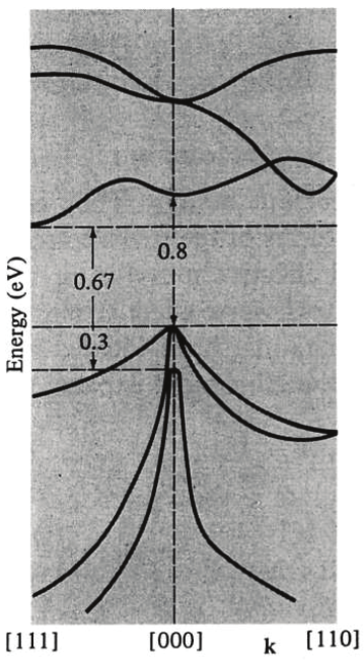
\includegraphics[height=0.5\textheight]{Figures/Electrodes/band_structure.pdf}
\caption{Scheme of the band structure in a germanium crystal.}
\label{fig:band-structure}
\end{figure}

\begin{figure}
\centering
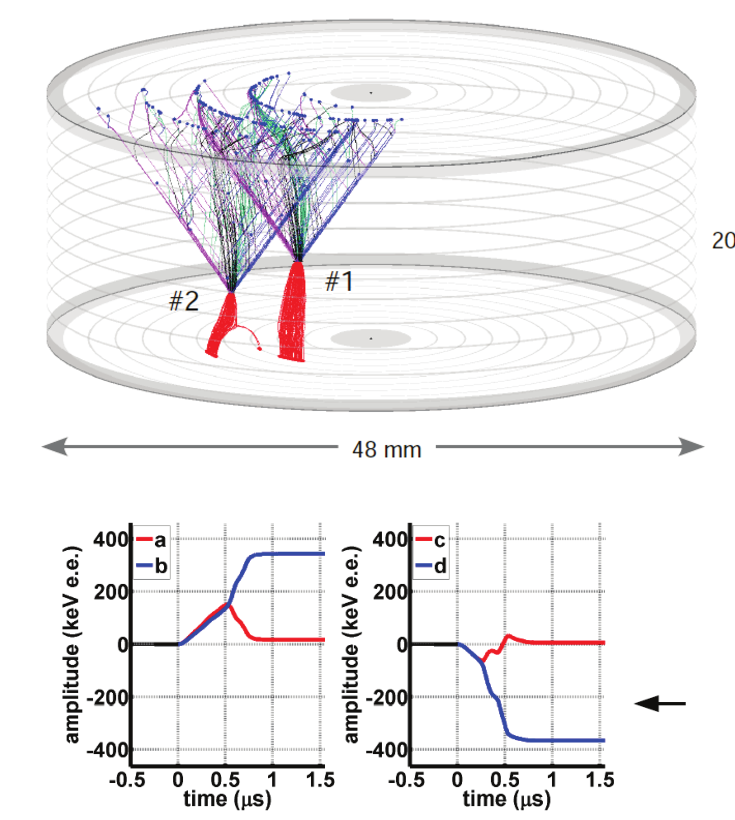
\includegraphics[height=0.5\textheight]{Figures/Electrodes/charge_drifting.pdf}
\caption{Scheme of the band structure in a germanium crystal.}
\label{fig:charge-drifting}
\end{figure}


\subsection{DAQ and electronics for ionization}

The electronics used for the ionization and the heat channel uses Junction Field Effect Transistor (JFET) which are operated at a low temperature of 100K inside the cryostat.
Some mumbo jumbo about the bolo-box (is it necessary ?).
The figure \ref{fig:electronics-scheme} show the scheme of the cold electronics for the heat channel (on the left) and the ionization channel (on the right).

\begin{figure}
\centering
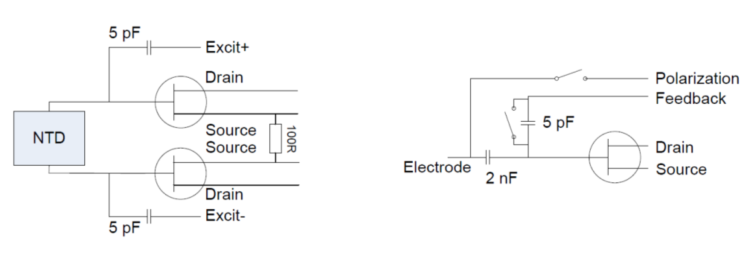
\includegraphics[width=\textwidth]{Figures/Electrodes/electronics_scheme.pdf}
\caption{Scheme of the cold electronics readout for the heat channel (left) and the ionization channel (right)}
\label{fig:electronics-scheme}
\end{figure}

In most experiments (source?), the ionization channel readout is done with the integration of the drifting charge current on the feedback capacitance of a charge amplifier. However, the EDELWEISS electronics directly measures the electric potential of the electrodes with a voltage amplifier. As each electrode is considered as a terminal of a capacitor $C_{electrode}$, the measured voltage is:
\begin{equation}
U = \frac{Q}{C_{electrode}}
\end{equation}
with $Q$ the drifting charge seen by the electrode.
Compare with a charge amplifier, the voltage amplifier does not involve any resistor in the amplification scheme, resulting a lower noise. However, the use of a voltage amplifier is only possible with a low leakage current, lower than 0.1fA (good for EDELWEISS, but is this possible for RICOCHET with operation on surface).

The ionization channel readout being based on the collection of electric charges, the renewal of the electric potential of the electrodes is necessary to maintain the voltage bias of the detector and to prevent the signal from leaving the readout range [-32000, +32000]. This operation, called a “reset”, consists in linking each electrodes to a polarization circuit of fixed electric potential. The linking is assured with mechanical relays (motivated by publication?) represented as a switch on the electronics scheme. The period of the resets is of a few seconds and should be adjusted empirically to the operated detectors and the event rates. In the case of surfaces operation at IP2I, the event rate is high and lot of charges are accumulated which needs for a shorter period than an underground operation at the LSM.
One should note the double switch of the mechanical relays accompanying each reset induces an artifact signal on both the heat and ionization channel. While easily discriminable from real events, these artifact signal result in dead time during which the detector is not available for valid event recording. Thus a short period of reset is not wanted.

While the majority of the electric charges produces by the ionization process are collected by the electrodes, some become trapped in the crystal (impurities) or on the surfaces of the crystal. These trapped charges are slowly accumulating and creating a counter electric field in the absorber. This results in a lower electric field perceived in the bulk of the detector which hampers a correct charge collection and decreases the sensitivity of the electrodes.
A procedure called “maintenance” is used to periodically shake up the trapped charges. These maintenances prevent, or at least slow significantly, the counter field build-up in the detector. A maintenance consists of a minute of multiples relay switches and relay changeovers. This procedure continuously invert the voltage bias in the detector, eventually destabilizing the trapped charges which are left to drift and collection in the electrodes.
During a maintenance, the detector is not available for data taking. The frequency of maintenance should be low to lower the dead time. For above ground operation, the usual maintenance period is of about 30 minutes and should be empirically adjusted to the detector and the event rate.

While a maintenance shakes up the majority of the trapped electric charges, a small fraction is not affected and participates to build up the counter field. These remaining charges are deeply trapped and need for a stronger perturbation to be freed. The detector is therefore periodically submitted to a procedure called "regeneration" aiming at a full reset of any passive electric field in the germanium crystal. With the electrodes being grounded, an intense gamma-ray radioactive source irradiates the detector. The high frequency of high energy recoils produces ionization in the whole crystal which eventually neutralize the accumulated space charges. 
As for the reset and maintenance procedures, the period between two regenerations should be empirically adjusted to the measured charge accumulation while not too frequent to avoid supplementary dead times. For above-ground operation, regeneration are realized ever two days (with a 1Cu cesium source).

Between each maintenance, the detector stays floating. The common noise can be subtracted when considering the charge conservation for all the electrodes:
\begin{equation}
\label{eq:charge-conservation}
A + B + C + D = 0
\end{equation}
With a linear combination of the raw ionization channels (A,B,C,D), we obtain new quantities (A’, B’, C’, D’) corrected from this common noise:
\begin{equation}
\label{eq:common-noise-subtraction}
A’ = \frac{3}{4} A - \frac{1}{4} \left( B + C + D \right)
\end{equation} 
The decrease of the noise level can be appreciated in the figure \ref{fig:ionization-noise} showing the noise spectrum affecting the different ionization channels before and after linear combination.

\begin{figure}
\centering
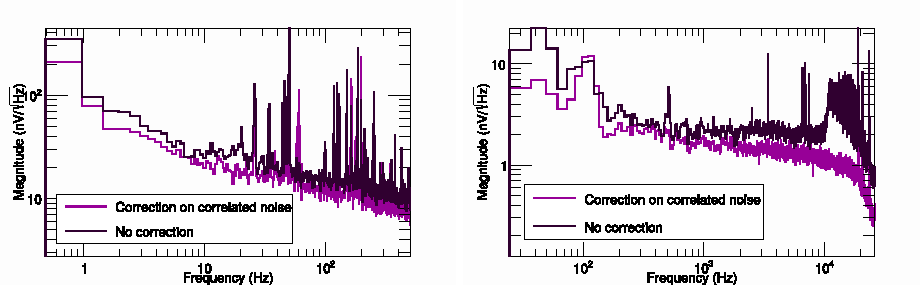
\includegraphics[width=\textwidth]{Figures/Electrodes/ionization_noise.pdf}
\caption{Average noise amplitude (in nV / Hz ) as a function of frequency of the
ionization channel for an EDELWEISS detector. The black histogram corresponds to the
noise before the correlated noise correction and the purple histogram to the noise after
the correction. Left: frequencies below 500 Hz. Right: high frequency part. [Emeline caption]}
\label{fig:ionization-noise}
\end{figure}

The ionization channel readout is sampled at an initial 100kHz. This means the period of the  measurement points is 10$\mu$s which greater than the estimated time span of an ionization signal of a few $\mu$s [ref necessary Alex.B ?]. As a result, an ionization signal is recorded as an Heaviside function. No information can be obtained on the shape of the signal.
The high readout sampling was historically chosen in EDELWEISS for the purpose of triggering on the ionization channel with a good temporal resolution (is it true ?). The highly sampled ionization signal is then averaged in order to produce a signal of frequency $f_s$ of about 400Hz. This lower sampling is able to record the information contained in the ionization Heaviside signal (its amplitude mainly) while being lightweight in term of disk space, which is essential considering the recording and processing resources at our disposal. The saved ionization signal of sampling frequency $f_s$ is composed of points which are averages of $100kHz/f_s$ points. The saved signal is therefore a skewed Heaviside-like function (more info needed? Is this work using this fact?).

Should I talk about the HEMT technology ? The expected resolution and noise level ?


\subsection{Aluminum Deposition}

*Stefanos biblio here.*

The electrodes of the detectors are made by depositing aluminium on the surface of the germanium crystal. The aluminium deposition is carried out by the research group at CSNSM at Orsay. The deposition processes are still being improved.

The germanium crystal is placed in vacuum chamber where its surface is altered with beams of vaporized atoms (hydrogen, aluminium, xenon…). 
In order to prevent the surface leakage, a highly resistive layer is created under the aluminium electrodes. It is a 60 to 80 nm deep amorphous layer of hydrogenated germanium.

Two techniques are used for the detectors presented in this work: evaporation with mask and the (photo)lithography.
A solid mask can set between the beam source and the crystal in order to shape the altered surface. In the case of concentric circular electrode, the mask (presented in figure {fig:mask-evaporation}) consists in several curved slits which allow the passage of vaporized aluminium. By rotating the mask during the process, the aluminium is deposited in a ring pattern on the germanium.
Another method to control the shape of the electrode is to use photolitography. First, the whole surface of the crystal is covered with a layer of aluminium. Then, the aluminium is coated with a chemically-protective wax. The negative of the electrode pattern is carved in the wax coating with the use of lasers (hence the name of the procedure). Once done, the germanium crystal face is immersed in chemical solution reactive with aluminium. Only the aluminium protected by the wax (patterned as the desired electrode design) is left on the surface. Finally, the wax coating is removed with an other chemical.

Advantages and Inconvenient of the 2 techniques ?
-Mask during evaporation is more precise and quicker but can only be use for simple patterns  with the cylindrical symmetry of the crystal.
-Photolitography is a longer process, and may be less precise (chemical attack of the aluminium?) but can be used for any pattern desired. Useful in the case of square grids.
- Also, some constraints on the minimum width of the electrodes ?

Leakage current exist on the surface of the crystal thanks to possible defects (ref edelweiss?). After depositing the electrodes, the bare germanium surfaces are etched with a XeF2 pulsed beam in vacuum chamber. The surface of the germanium is altered according to the following equation:
$$Ge + 2XeF_2 \longrightarrow GeF_4 + 2Xe$$
The xenon gas is removed and the fluoarated germanium surface is able to hold much higher voltage bias.

Now that the aluminium electrodes were deposited on the germanium crystal, it is possible to proceed with the cabling. The fragility of the germanium and the shallow aluminium layers motivate the use of wire-bonding as cabling technique. 

*description wire-bonding machine*

In the case of simple electrodes (full planar detector), several wires link the top (and bottom) electrodes to a conductive pad on the detector copper chassis. The conductive pad is then cabled to the ionization electronics.
With more complex design (fully interdigitized), wires are used to connect different aluminium patches, essentially imposing the same electric potential is those. With two wire bridges, It is possible to create interleaved electrodes with a biasing scheme based on the co-planar grid technique for event localisation [ref emeline 86], but more on that later.


\subsection{Luke Neganov effect}

When electric charges drift under the influence of the applied electric field in the germanium crystal, phonons are created and eventually participate to the heat signal. This process is called the Luke-Neganov [ref 63 emeline]. This phenomenon happening in semi-conductors is analogous to the Joule Effect present in conductors. 
The drifting electrons constantly dissipate their energy to the phonons bath. As the electrons stay in motion and are eventually collected by the electrodes, the electric field must provide a work $W$ compensating the energy loss going into the heat channel.
This work required for a single electron-hole pair is expressed as:
\begin{align}
W &= q_{e^{-}} \int_{ \vec{r_i} }^{ \vec{r_{e,f}} } \vec{E} d\vec{r} - q_{h^{+}} \int_{ \vec{r_i} }^{ \vec{r_{h,f}} } \vec{E} d\vec{r} \\
&=  -e \int_{ \vec{r_i} }^{ \vec{r_{e,f}} } \frac{\partial V}{\partial \vec{r}} d\vec{r} + e \int_{ \vec{r_i} }^{ \vec{r_{h,f}} } \frac{\partial V}{\partial \vec{r}} d\vec{r} \\
&= e \left( V(\vec{r_{h,f}}) - V(\vec{r_{e,f}}) \right)
\end{align}
where $q_{e^{-}} = e = - q_{h^{+}} $ represent the electric charges and $\vec{r_{i,f}}$ is the final position of the electric charge $i \in \{e^{-}, h^{+}\}$. Therefore, the energy generated by the Luke-Neganov (for a single pair) depends solely on the electric potential at the end of drift positions for the electron $\vec{r_{e,f}}$ and the hole $\vec{r_{h,f}}$.


The Luke-Neganov effect boosts the heat channel by adding a Luke-Neganov energy $E_{Luke-Neganov}$. For a recoil of type $j \in \{ e, n\}$ generating a number of electron-pairs $N^j$, the expression of this energy is:
\begin{equation}
E_{Luke-Neganov} = e \sum_{i=0}^{N^j} \left( V(\vec{r_{h,f}^i}) - V(\vec{r_{e,f}^i}) \right)
\end{equation}
A useful, and mostly accurate, approximation is to consider that all the charges end their drift by being collected at the electrodes polarized at potential $V_+$ and $V_-$. Thus, a simpler expression of the boost in energy is:
\begin{equation}
E_{Luke-Neganov} = N^j e (V_+ - V_-) = N^j e \Delta V
\end{equation}
The Luke-Neganov effect is proportional to the number of pairs $N^j$ created in the ionization process and the voltage bias $\Delta V$ of the detector. Using the equation \ref{eq:number-pairs}, we can express the boost as a function of the recoil energy $E_R$ and the associated quenching factor $Q^j$:
\begin{equation}
E_{Luke-Neganov} = Q^j \frac{E_R}{\epsilon} e \Delta V
\end{equation}
A useful simplification is to consider that $e / {\epsilon} = 1/3 \textsf{V}^{-1}$,  and to have a final expression of the Luke-Neganov boost as:
\begin{equation}
\label{eq:nl-boost}
E_{Luke-Neganov} = Q^j E_R \frac{\Delta V}{3}
\end{equation}
We see that for the same recoil energy $E_R$, an electronic recoil will benefits more than a nuclear recoil from the boost according to the comparison of  their quenching factor $Q^e > Q^n$. This is very important to keep in mind when reconstructing the recoil energy $E_R$ from the measured heat energy $E_{heat}$ as it is a function of the deposited recoil energy $E_R$ and the recoil type $j$:
\begin{align}
E_{heat} (E_R, j ) &= E_{R} + E_{Luke-Neganov} ( E_R, j) \\
&= E_R \left( 1 + Q^j(E_R) \frac{\Delta V}{3} \right)
\end{align}

*more on that now or later ? Kevee, kevnr, use of the Ei and Ec to deduce Q and Er*


\subsection{Shockley–Ramo theorem}

[ref quentin 100 101 102]
The signal induced on the electrodes of a detector does not corresponds to the collection of the drifting charges (when the charges reach the electrodes) but rather corresponds to the induced current starting from the moment the electron-pairs are created by a recoil. Indeed, when a charge is moving in the vicinity of an electrode, it induces an instantaneous electric current by affecting the electrostatic field lines ending on the electrode. 
[wiki after]
The Shockey-Ramo theorem states that the current $i$ induced on a given electrode due to the motion of a charge is given by:
\begin{equation}
I = E_v q v
\end{equation}
where $q$ is the charge of the particle, $v$ its velocity and $E_v$ the component of the electric field in the direction of $v$, under the following conditions: charge removed, given electrode raised to unit potential, and all other conductors grounded. This theorem ensues from Gauss theorem.
This theorem can be integrated to access the induced charge on a given electrode $k$:
\begin{equation}
Q_k = - q \Phi_k(\vec{r})
\end{equation}
with $\Phi_k(\vec{r})$ the weighted potential of the electrode $k$. This weighted potential is obtained in the same conditions as $E_v$. (figure of such potential for an electrode?).
In the case of a drifting charge $q$ of initial position $\vec{r_{q,i}}$ and final position $\vec{r_{q,f}}$, the total integrated charge induced on the electrode $k$ is:
\begin{equation}
Q_k = q \left( \Phi_k (\vec{r_{q,f}}) - \Phi_k (\vec{r_{q,i}}) \right)
\end{equation}
The Shocley-Ramo theorem benefits from the superposition theorem such that it is possible to express the signal induced by a number $N$ of electron-hole pairs:
\begin{align}
Q_k &= \sum_{n=1}^{N} \left( Q_k^n(e^-) + Q_k^n(h^+) \right) \\
&= \sum_{n=1}^{N} -e \left( \Phi_k^n (\vec{r_{e,f}}) - \Phi_k^n (\vec{r_{e,i}}) \right) +e \left( \Phi_k^n (\vec{r_{h,f}}) - \Phi_k^n (\vec{r_{h,i}}) \right)
\end{align}
When considering the drifting of a single electron-hole pair, the initial position is the same for both charges and thus: $\Phi_k (\vec{r_{e,i}}) = \Phi_k (\vec{r_{h,i}})$.
The signal induced by $N$ electron-hole pairs is simplified to:
\begin{equation}
Q_k = e \sum_{n=1}^{N} \left( \Phi_k^n (\vec{r_{e,f}}) - \Phi_k^n (\vec{r_{h,f}}) \right)
\end{equation}
It solely depends on the weighted potential of the final position of the charges. While the vast majority of charges ends up collected in the electrodes and participate with a weighted potential of $\pm 1$, some charges are trapped and so participate to the signal with the weighted potential corresponding to the position of the trap, which reduces the induced signal.
If the electrodes of the detector form a Faraday cage, all the field lines end on the electrodes and none is leaving the crystal. As a result, when considering a unique charge $q$ in the crystal, the total weighted potential $Q_T$ is:
\begin{equation}
\label{eq:charge-conservation}
Q_T = Q_A + Q_B + Q_C + Q_D = -q
\end{equation}
When considering $N$ electron-holes pairs, the Faraday cage imposes the charge conservation:
\begin{equation}
\label{eq:charge-conservation}
Q_T = Q_A + Q_B + Q_C + Q_D = \sum_{n=1}^{N} e (1 – 1) = 0
\end{equation}

Should I include the study of the trapping by Quentin ? Some studies [103 and 104 quentin ref] were done on the dependance of the electric charge  trapping in germanium crystals. Electrons are more prone to be trapped than hole. According ti Quentin, 10 to 20% of the carriers are trapped (?). He then calculates the signal induced with trapping and also the effect of trapping as a function of the trap localization. And the impact of trapping on the heat channel.



\subsection{Objective of the electrode study}

Produce a good design of electrodes for 32g/38g ge detectors
Objectives:
Low capacitance
High fiducial volume
Good charge collection


\section{Of the use of Comsol}

\subsection{Axy-symmetrical} 

Let's talk about the fact that I used 2D simulation which is then rotated to form a 3D simulation of cylindrical symmetry.

2D simulations are quicker than 3D simulation.
According to some quick tests, the simulation of a given geometry is the same in 3D or 2D.
So yeah, using that.

Maybe, search in the comsol manual and see how this is done in the equations.
TO BE DONE.

\begin{figure}
\centering
\begin{subfigure}{.5\textwidth}
  \centering
  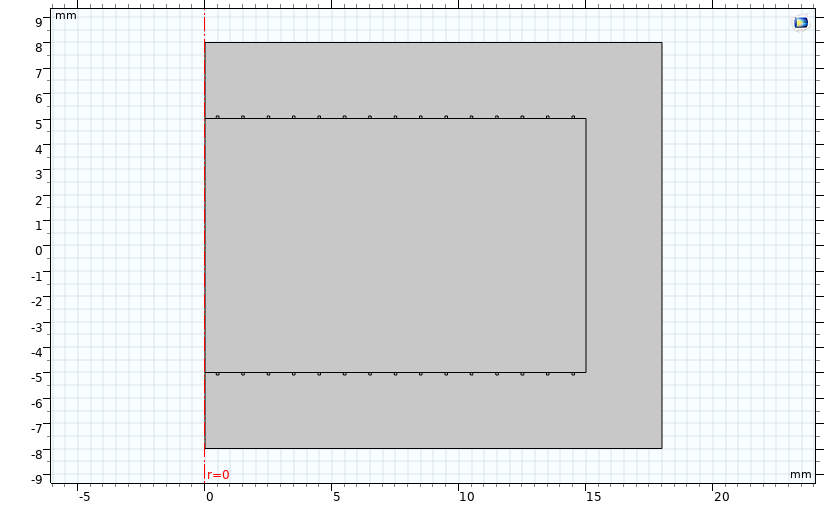
\includegraphics[width=\linewidth]{Figures/Electrodes/2D_simulation.png}
  \caption{Simulation of the concentric grid planar in 2D-axisymmetry with COMSOL.}
  \label{fig:2D-simulation}
\end{subfigure}%
\begin{subfigure}{0.5\textwidth}
  \centering
  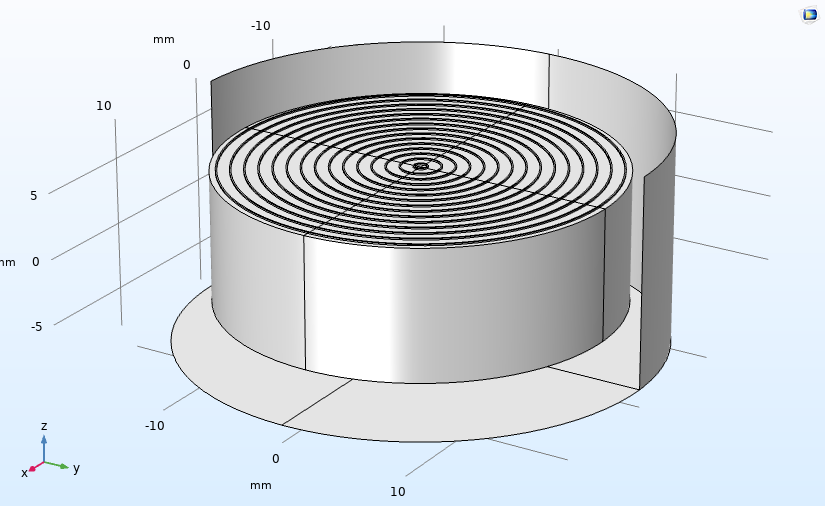
\includegraphics[width=\linewidth]{Figures/Electrodes/3D_simulation.png}
  \caption{Simulation of the concentric grid planar in 3D with COMSOL.}
  \label{fig:3D-simulation}
\end{subfigure}
\caption{To illustrate the differences between 2D and 3D.}
\label{fig:2D-vs-3D}
\end{figure}

\subsection{Building the geometry}

Assomptions used for the simulation (like perfect cylindrical symmetry)
No simulation of the NTD, just test in 3D, no impact if put on electrode, but discussion and checking are necessary for that.

\subsection{Meshing}

Did I told you that comsol is a finte elements software ? no ? well, it is !
These finite elements are small section of the geometric space where the calculationb of the physics quantities are calculated discritely. These finite elements are defined by the meshing, which divide the space. However, there is a way to divide space more efficiently than others. Like attribuating large portion of space where the physical quantities are quite constant and small portions where they are prone to a lot of fluctuation.
And guess what I did with this fabulous option ?
yeah, I kept it on full automatic for physics. Guess I should dig a bit deeper to see what this is all about. Like, size a mesh simplex according to the smallest feature in the geometry and things like that.
TO BE DONE.

\subsection{Capacitance Calculation}

Everybody know that the capacitance $C$ links the voltage of an electrode $V$ and $Q$ the  charges accumulated in this electrode:
\begin{equation}
C \times U = Q
\end{equation}

This is quite basic, but no so evident when their is more than two electrodes with different electric potential in a system. That is why it is hopefully possible to generalized the notion of capacitance to more electrodes with the lumped matrix capacity or the Maxwell capacity matrix (consider whatever suits you, they mean the same).

INSERT MATRIX HERE

\begin{figure}
\centering
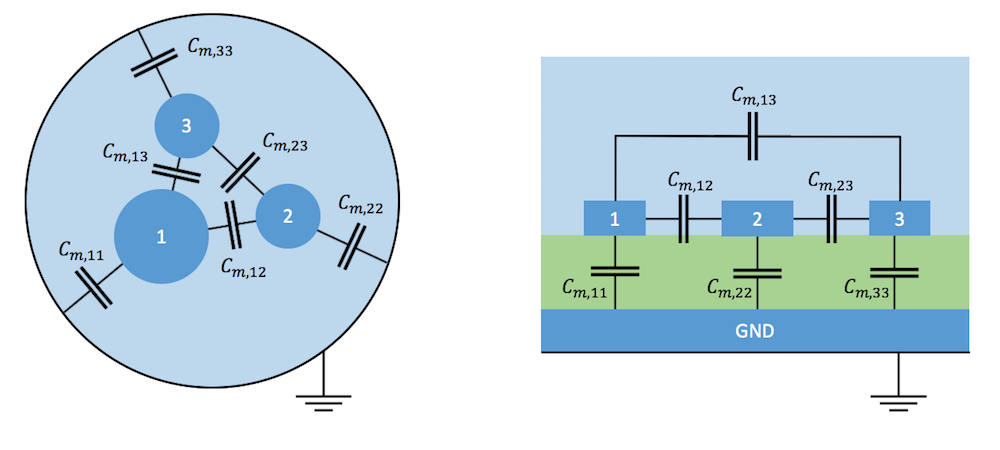
\includegraphics[width=\linewidth]{Figures/Electrodes/lumped_capacitance_scheme.png}
\caption{Scheme representing the capacitance between each electrodes in electric field simulation.}
\label{fig:lumped-capacitance}
\end{figure}

How does comsol calculate this lumped capacitance matrix ?
Well, it considers the equation i just wrote before, and fixes all except one electrode to zero and sweep over the electrodes with 1V of potential. Just with that, the software is able to deduce all the terms of the matrix.
Yeah, i should read more about that in the manual to see if this is done like that. But it is. yep.
TO BE DONE.


CROSSTALK
Yep, gotta talk about the link between the crosstalk on the ionization channels and the capacitance term between those electrodes.
We can simply say for now that the higher the capacitance is and the higher the crosstalk will be. However, it should be very interesting to quantify the link between these two quantities.
Linking the crosstalk matrix and the capacitance matrix, and be able to compare that experimentally.

ANALYSIS TO BE DONE


\subsection{Estimation of the Theoretical Fiducial Volume}

In this subsection, i explain how to estimate the fiducial volume.
Draw streamlines crossing the z=0.
Exporting to image png.
Using graphical analysis with python and rescaling to take into account 2D-axisymmetry.

\begin{figure}
\centering
\begin{subfigure}{.5\textwidth}
  \centering
  \includegraphics[width=\linewidth]{Figures/Electrodes/streamlines_comsol.png}
  \caption{Drawing streamlines in COMSOL}
  \label{fig:streamlines-comsol}
\end{subfigure}%
\begin{subfigure}{0.5\textwidth}
  \centering
  \includegraphics[width=\linewidth]{Figures/Electrodes/streamlines_corrected.png}
  \caption{for 4*4mm NTD}
  \label{fig:streamlines-corrected}
\end{subfigure}
\caption{Illustration of the estimation of the fiducial volume.}
\label{fig:fiducial-volume-estimation}
\end{figure}

\subsection{General region for the charge collection in a detector}

WITH A SCHEME
To illustrate the different region of the detector differing by the expected charge collection.

\begin{itemize}
	\item collecting zone
	\item veto zone
	\item guard zone
	\item lost zone (streamlines exiting the crystal)
	\item in between all of them, either low electric field (bad for trapping and recombination) or unclear frontier (when thinking of the recoil as a charged firework).
\end{itemize}

\section{Simulated Configurations}

In this section, I will talk about the different configurations that were simulated.
These configurations can differ according to the mass of the crystal, the number of electrodes, the position and geometry of the electrodes.
Maybe, i should describe the configurations in a kind of general way: planar, grid, ID, FID, etc.. and put the exact simulation of each detectors in the annexes. I dont really know yet.

\subsection{Planar Geometry}

(Like REDN1 or RED80, with planar polarization, not much runs)

\subsubsection{Full Planar}

Maxwell Capacitance: $11.88 \times 10^{-12}$F

\begin{figure}
\centering
\includegraphics[width=\linewidth]{Figures/Electrodes/full_planar.png}
\caption{Scheme of the simulated full planar h10phi30 detector.}
\label{fig:full-planar}
\end{figure}

\subsubsection{Concentric/Square Grid Planar}

Maxwell Capacitance: $11.88 \times 10^{-12}$F

\begin{figure}
\centering
\includegraphics[width=\linewidth]{Figures/Electrodes/concentric_grid_planar.png}
\caption{Scheme of the simulated concentric grid planar h10phi30 detector.}
\label{fig:concentric-grid-planar}
\end{figure}

\subsection{Planar with Guard}

Like RED80, many runs.

\subsection{Interdigitized}

Like REDN1, many runs.

Lot of different variants here.

On the presented figure, the central pad is chosen to be polarized at veto potential and the NTD thermal sensor should be glued on it.

\begin{figure}
\centering
\includegraphics[width=\linewidth]{Figures/Electrodes/ID_geometry.png}
\caption{Scheme of the simulated interdigitized detector.}
\label{fig:concentric-grid-planar}
\end{figure}

\subsection{Fully Interdigitized}

Like RED70 (no run, RIP)

Presenting the FID geometry, with veto zone, collect, zone and the faraday cages effect which means that the charge collection is *really* good.

\begin{figure}
\centering
\includegraphics[width=\linewidth]{Figures/placeholder.jpg}
\caption{Illustrating the veto zone and the collect zone thanks to the electric field shape induced by the FID electrodes.}
\label{fig:fid-illustration}
\end{figure}

\subsection{Comparing the different topologies}

\begin{table}[]
\centering
\resizebox{\linewidth}{!}{
	\begin{tabular}{ |c||c|c|c|c|c| }
	\hline 
	Topology & Capacitance $[pF]$ & Fiducial $[\%]$ & Surface Tagging & Charge Collection & Other characteristics \\ \hline
	
	Full Planar & $\approx 10$ & $\approx 90$ & No & Side:No & HO on Al? \\ \hline
	Grid Planar & $\approx 10$ & $\approx 80$ & No & Side:No & Collect near Al? \\ \hline
	ID & 8 to 25 &  45 to 55 & Yes* & Center/Side: ??? & -- \\ \hline \hline
	FID & $> 25$ to $\approx 100$ & 50 to 80 & Yes & Very Good & -- \\	 
	\hline
\end{tabular}
}
\caption{Sum-up of the performance and specificity of each electrode topology.}
\label{tab:stream-glitch-time-cut}
\end{table}

\section{Influence of parameters}

For each parameter, we want to study their impact on the performances of the detector.
The fiducial volume, the electric field shape, the electric field norm and the capacitance.

The fiducial volume is a number.
The electric field shape/norm is one or two graphs.
The capacitance is a matrix (non-diagonal term are useful to estimate the coupling between each electrodes)

\subsection{Capacitance with chassis distance}

*All topologies*

The capacitance term between the electrodes and the ground decreases with the distance of the copper chassis. As expected by the capacitance formula of a plan capacitor.
The capacitance term capa-capa tends to the expected value for a plan capacitor in empty space.

\begin{figure}
\centering
\includegraphics[width=\linewidth]{Figures/Electrodes/capacitance_chassis_distance.png}
\caption{Graph of the capacitance terms in function of the distance between the Ge crystal and the copper chassis (concentric grid planar h10phi30 detector).}
\label{fig:capcaitance-chassis-distance}
\end{figure}

\subsection{Capacitance with electrode spacing}

*All topologies except full planar*

The electrode spacing directly fixes the number of concentric circle on a plan face of the germanium crystal. As a result the curves show a saw-shaped profile corresponding to the discrete number of electrodes.
Anyway, the global trend is that with a high spacing, there is less electrodes and less capacitance.

This tells us that we want to reduce the surface of electrode on the crystal in order to decrease the capacitance. However, a lower surface of electrodes comes with a worse charge collection eventually. So trade-off time.

\begin{figure}
\centering
\includegraphics[width=\linewidth]{Figures/Electrodes/capacitance_electrode_spacing.png}
\caption{Graph of the capacitance terms in function of the electrode spacing (concentric grid planar h10phi30 detector).}
\label{fig:capacitance-electrode-spacing}
\end{figure}

\begin{figure}
\centering
\begin{subfigure}{.5\textwidth}
  \centering
  \includegraphics[width=\linewidth]{Figures/Electrodes/2x2_distance_sweep.png}
  \caption{for 2*2mm NTD}
  \label{fig:2D-simulation}
\end{subfigure}%
\begin{subfigure}{0.5\textwidth}
  \centering
  \includegraphics[width=\linewidth]{Figures/Electrodes/4x4_distance_sweep.png}
  \caption{for 4*4mm NTD}
  \label{fig:3D-simulation}
\end{subfigure}
\caption{Graph of the capacitance terms in function of the electrode spacing (interdigitized).}
\label{fig:2D-vs-3D}
\end{figure}

I could also mention the projection for the fid32 and fid38 that were simulated with different electrode spacing.

\begin{table}[]
\centering
\resizebox{\linewidth}{!}{
	\begin{tabular}{|c|c|c|c|c|c|c|c|}
\hline
Lateral $[mm]$ & \begin{tabular}[c]{@{}c@{}}Lateral Elec.\\ Veto/Collect\end{tabular} & Plan $[mm]$ & \begin{tabular}[c]{@{}c@{}}Plan Elec.\\ Veto/Collect\end{tabular} & $\%_{fiducial}$ & $C_{veto} [pF]$ & $C_{collect} [pF]$ & Comments \\ \hline
 &  &  & 4c / 3 & 63 & 21.5 & 18.8 & OK \\
 &  &  & {\color[HTML]{FE0000} 3 / 4c} & {\color[HTML]{FE0000} 66} & {\color[HTML]{FE0000} 20.4} & {\color[HTML]{FE0000} 18.4} & {\color[HTML]{FE0000} Collect} \\
 &  & \multirow{-3}{*}{1.4} & {\color[HTML]{3166FF} 4o / 4c} & {\color[HTML]{3166FF} 66} & {\color[HTML]{3166FF} 22.9} & {\color[HTML]{3166FF} 20.1} & {\color[HTML]{3166FF} Special} \\  \cline{3-8} 
 &  &  & {\color[HTML]{FE0000} 3c / 3} & {\color[HTML]{FE0000} 66} & {\color[HTML]{FE0000} 19.3} & {\color[HTML]{FE0000} 17.3} & {\color[HTML]{FE0000} Collect} \\
 &  &  & {\color[HTML]{3166FF} 3c / 4o} & {\color[HTML]{3166FF} 64} & {\color[HTML]{3166FF} 21.8} & {\color[HTML]{3166FF} 19.1} & {\color[HTML]{3166FF} Special} \\
 &  & \multirow{-3}{*}{1.7} & 3 / 3c & 62 & 20.4 & 17.8 & OK \\ \cline{3-8} 
 &  &  & 3c / 2 & 61 & 19.3 & 16.7 & OK \\
 &  &  & {\color[HTML]{FE0000} 2 / 3c} & {\color[HTML]{FE0000} 64} & {\color[HTML]{FE0000} 18.2} & {\color[HTML]{FE0000} 16.2} & {\color[HTML]{FE0000} Collect} \\
\multirow{-9}{*}{1.6} & \multirow{-9}{*}{3 / 3} & \multirow{-3}{*}{2.1} & {\color[HTML]{3166FF} 3o / 3c} & {\color[HTML]{3166FF} 62} & {\color[HTML]{3166FF} 20.7} & {\color[HTML]{3166FF} 18.0} & {\color[HTML]{3166FF} Special} \\ \hline
 &  &  & {\color[HTML]{009901} 4c / 3} & {\color[HTML]{009901} 57} & {\color[HTML]{009901} 18.6} & {\color[HTML]{009901} 15.1} & {\color[HTML]{009901} Veto} \\
 &  &  & {\color[HTML]{3166FF} 4c / 4o} & {\color[HTML]{3166FF} 61} & {\color[HTML]{3166FF} 20.4} & {\color[HTML]{3166FF} 17.6} & {\color[HTML]{3166FF} Special} \\
 &  & \multirow{-3}{*}{1.4} & 3 / 4c & 61 & 19.1 & 16.3 & OK \\ \cline{3-8} 
 &  &  & 3c / 3 & 60 & 18.0 & 15.3 & OK \\ 
 &  &  & {\color[HTML]{009901} 3 / 3c} & {\color[HTML]{009901} 57} & {\color[HTML]{009901} 17.5} & {\color[HTML]{009901} 14.0} & {\color[HTML]{009901} Veto} \\
 &  & \multirow{-3}{*}{1.7} & {\color[HTML]{3166FF} 3 / 4co} & {\color[HTML]{3166FF} 60} & {\color[HTML]{3166FF} 19.4} & {\color[HTML]{3166FF} 16.6} & {\color[HTML]{3166FF} Special} \\ \cline{3-8} 
 &  &  & {\color[HTML]{009901} 3c / 2} & {\color[HTML]{009901} 56} & {\color[HTML]{009901} 16.4} & {\color[HTML]{009901} 12.9} & {\color[HTML]{009901} Veto} \\
 &  &  & {\color[HTML]{3166FF} 3c / 3o} & {\color[HTML]{3166FF} 59} & {\color[HTML]{3166FF} 18.2} & {\color[HTML]{3166FF} 15.5} & {\color[HTML]{3166FF} Special} \\ 
\multirow{-9}{*}{2.0} & \multirow{-9}{*}{3 / 2} & \multirow{-3}{*}{2.1} & 2 / 3c & 58 & 17.0 & 14.1 & OK \\ \hline
\end{tabular}
}
\caption{Projection of the FID32 design performance with multiple variants (collect at $\pm4$V, veto at $\mp1.5$V)}
\label{tab:stream-glitch-time-cut}
\end{table}

\begin{table}[]
\centering
\resizebox{\linewidth}{!}{
	\begin{tabular}{|c|c|c|c|c|c|c|c|}
\hline
Lateral $[mm]$ & \begin{tabular}[c]{@{}c@{}}Lateral Elec.\\ Veto/Collect\end{tabular} & Plan $[mm]$ & \begin{tabular}[c]{@{}c@{}}Plan Elec.\\ Veto/Collect\end{tabular} & $\%_{fiducial}$ & $C_{veto} [pF]$ & $C_{collect} [pF]$ & Comments \\
\hline
 					  & 						& 					    & 6c / 5 & 71 & 34.8 & 30.5 & OK \\
 					  & 						& 						& {\color[HTML]{FE0000}5 / 6c} & {\color[HTML]{FE0000}75} & {\color[HTML]{FE0000}33.2} & {\color[HTML]{FE0000}30.4} & {\color[HTML]{FE0000}Collect} \\
 					  & 						& \multirow{-3}{*}{1.3} & {\color[HTML]{3166FF} 6o / 6c} & {\color[HTML]{3166FF} 73} & {\color[HTML]{3166FF} 36.8} & {\color[HTML]{3166FF} 32.6} & {\color[HTML]{3166FF} Special}\\
\cline{3-8} 
 					  & 						& 					    & {\color[HTML]{FE0000}5c / 5} & {\color[HTML]{FE0000}74} & {\color[HTML]{FE0000}31.7} & {\color[HTML]{FE0000}28.8} & {\color[HTML]{FE0000}Collect} \\
 					  & 						& 					    & {\color[HTML]{3166FF}6c / 5} & {\color[HTML]{3166FF} 72} & {\color[HTML]{3166FF}35.6} & {\color[HTML]{3166FF}31.4} & {\color[HTML]{3166FF}Special} \\
 					  & 						& \multirow{-3}{*}{1.5} & 5o / 5c & 71 & 33.5 & 29.2 & OK\\
\cline{3-8} 
 					  & 						& 					    & 5c / 4 & 70 & 31.1 & 26.8 & OK \\
 					  & 						& 					    & {\color[HTML]{FE0000}4 / 5c} & {\color[HTML]{FE0000}74} & {\color[HTML]{FE0000}29.5} & {\color[HTML]{FE0000}26.8} & {\color[HTML]{FE0000}Collect} \\
 					  & 						& \multirow{-3}{*}{1.6} & {\color[HTML]{3166FF}5o / 5c} & {\color[HTML]{3166FF}72} & {\color[HTML]{3166FF}33.2} & {\color[HTML]{3166FF}29.0} & {\color[HTML]{3166FF}Special} \\
\cline{3-8} 
 					  & 						& 					    & {\color[HTML]{FE0000}4c / 4} & {\color[HTML]{FE0000}74} & {\color[HTML]{FE0000}27.6} & {\color[HTML]{FE0000}25.1} & {\color[HTML]{FE0000}Collect} \\
 					  & 						& 					    & {\color[HTML]{3166FF}5co / 4} & {\color[HTML]{3166FF}71} & {\color[HTML]{3166FF}31.3} & {\color[HTML]{3166FF}27.3} & {\color[HTML]{3166FF}Special} \\
 					  & 						& \multirow{-3}{*}{1.8} & 4 / 4c & 68 & 29.3 & 25.0 & OK \\
\cline{3-8} 
 					  & 						& 					    & 4c / 3 & 67 & 27.6 & 23.5 & OK \\
 					  & 						& 					    & {\color[HTML]{FE0000}3 / 4c} & {\color[HTML]{FE0000}72} & {\color[HTML]{FE0000}26.1} & {\color[HTML]{FE0000}23.5} & {\color[HTML]{FE0000}Collect} \\
\multirow{-15}{*}{1.1} & \multirow{-15}{*}{2 / 2} & \multirow{-3}{*}{2.1} & {\color[HTML]{3166FF}4o / 4c} & {\color[HTML]{3166FF}69} & {\color[HTML]{3166FF}29.8} & {\color[HTML]{3166FF}25.6} & {\color[HTML]{3166FF}Special} \\

\hline

 					  & 					  & 					  & {\color[HTML]{009901}6c / 5} & {\color[HTML]{009901}64} & {\color[HTML]{009901}30.0} & {\color[HTML]{009901}24.3} & {\color[HTML]{009901}Veto} \\
 					  & 					  & 					  & {\color[HTML]{3166FF}6c / 6o} & {\color[HTML]{3166FF}68} & {\color[HTML]{3166FF}32.4} & {\color[HTML]{3166FF}28.2} & {\color[HTML]{3166FF}Special} \\
 					  & 					  & \multirow{-3}{*}{1.3} & 5 / 6c & 70 & 30.3 & 26.1 & OK \\
\cline{3-8} 
 					  & 					  & 					  & 5c / 5 & 69 & 28.9 & 24.9 & OK \\
 					  & 					  & 						& {\color[HTML]{009901}5 / 5c} & {\color[HTML]{009901}65} & {\color[HTML]{009901}28.4} & {\color[HTML]{009901}22.8} & {\color[HTML]{009901}Veto} \\
 					  & 						& \multirow{-3}{*}{1.5} & {\color[HTML]{3166FF}5 / 6co} & {\color[HTML]{3166FF}67} & {\color[HTML]{3166FF}31.3} & {\color[HTML]{3166FF}26.9} & {\color[HTML]{3166FF}Special} \\
\cline{3-8} 
 					  & 					  & 						& {\color[HTML]{009901}5c / 4} & {\color[HTML]{009901}62} & {\color[HTML]{009901}26.4} & {\color[HTML]{009901}20.5} & {\color[HTML]{009901}Veto} \\
 					  & 					  & 					  & {\color[HTML]{3166FF}5c / 5o} & {\color[HTML]{3166FF}66} & {\color[HTML]{3166FF}28.7} & {\color[HTML]{3166FF}24.5} & {\color[HTML]{3166FF}Special} \\
 					  & 					  & \multirow{-3}{*}{1.6} & 4 / 5c & 68 & 26.6 & 22.4 & OK \\
\cline{3-8} 
 					  & 					  & 					  & 4c / 4 & 67 & 24.7 & 20.6 & OK \\
 					  & 					  & 						& {\color[HTML]{009901}4 / 4c} & {\color[HTML]{009901}60} & {\color[HTML]{009901}24.7} & {\color[HTML]{009901}18.7} & {\color[HTML]{009901}Veto} \\
 					  & 						& \multirow{-3}{*}{1.8} & {\color[HTML]{3166FF}4 / 5co} & {\color[HTML]{3166FF}64} & {\color[HTML]{3166FF}27.0} & {\color[HTML]{3166FF}22.6} & {\color[HTML]{3166FF}Special} \\
\cline{3-8} 
 					  & 					  & 						& {\color[HTML]{009901}4c / 3} & {\color[HTML]{009901}59} & {\color[HTML]{009901}23.1} & {\color[HTML]{009901}17.1} & {\color[HTML]{009901}Veto} \\
 					  & 					  & 					  & {\color[HTML]{3166FF}4c / 4o} & {\color[HTML]{3166FF}63} & {\color[HTML]{3166FF}25.3} & {\color[HTML]{3166FF}21.1} & {\color[HTML]{3166FF}Special} \\
\multirow{-15}{*}{1.6} & \multirow{-15}{*}{2 / 1} & \multirow{-3}{*}{2.1} & 3 / 4c & 66 & 23.2 & 19.0 & OK \\

\hline

 					  & 						& 					    & 6c / 5 & 68 & 26.1 & 22.5 & OK \\
 					  & 					  & 						& {\color[HTML]{FE0000}5 / 6c} & {\color[HTML]{FE0000}73} & {\color[HTML]{FE0000}24.2} & {\color[HTML]{FE0000}22.6} & {\color[HTML]{FE0000}Collect} \\
 					  & 						& \multirow{-3}{*}{1.3} & {\color[HTML]{3166FF}6o / 6c} & {\color[HTML]{3166FF}70} & {\color[HTML]{3166FF}28.0} & {\color[HTML]{3166FF}24.6} & {\color[HTML]{3166FF}Special} \\
\cline{3-8} 
 					  & 					  & 						& {\color[HTML]{FE0000}5c / 5} & {\color[HTML]{FE0000}72} & {\color[HTML]{FE0000}22.7} & {\color[HTML]{FE0000}21.1} & {\color[HTML]{FE0000}Collect} \\
 					  & 					  & 					  & {\color[HTML]{3166FF}6co / 5} & {\color[HTML]{3166FF}69} & {\color[HTML]{3166FF}26.8} & {\color[HTML]{3166FF}23.4} & {\color[HTML]{3166FF}Special} \\
 					  & 					  & \multirow{-3}{*}{1.5} & 5 / 5c & 67 & 24.8 & 21.1 & OK \\
\cline{3-8} 
 					  & 						& 					    & 5c / 4 & 66 & 22.4 & 18.8 & OK \\
 					  & 					  & 						& {\color[HTML]{FE0000}4 / 5c} & {\color[HTML]{FE0000}72} & {\color[HTML]{FE0000}20.5} & {\color[HTML]{FE0000}19.0} & {\color[HTML]{FE0000}Collect} \\
 					  & 						& \multirow{-3}{*}{1.6} & {\color[HTML]{3166FF}5o / 5c} & {\color[HTML]{3166FF}68} & {\color[HTML]{3166FF}24.3} & {\color[HTML]{3166FF}20.9} & {\color[HTML]{3166FF}Special} \\
\cline{3-8} 
 					  & 					  & 						& {\color[HTML]{FE0000}4c / 4} & {\color[HTML]{FE0000}72} & {\color[HTML]{FE0000}18.6} & {\color[HTML]{FE0000}17.3} & {\color[HTML]{FE0000}Collect} \\
 					  & 					  & 					  & {\color[HTML]{3166FF}5co / 4} & {\color[HTML]{3166FF}68} & {\color[HTML]{3166FF}22.4} & {\color[HTML]{3166FF}19.1} & {\color[HTML]{3166FF}Special} \\
 					  & 					  & \multirow{-3}{*}{1.8} & 4 / 4c & 64 & 20.6 & 17.0 & OK \\
\cline{3-8} 
 					  & 					  & 						& 4c / 3 & 63 & 19.0 & 15.5 & OK \\
 					  & 					  & 						& {\color[HTML]{FE0000}3 / 4c} & {\color[HTML]{FE0000}70} & {\color[HTML]{FE0000}17.0} & {\color[HTML]{FE0000}15.6} & {\color[HTML]{FE0000}Collect} \\
\multirow{-15}{*}{2.4} & \multirow{-15}{*}{1 / 1} & \multirow{-3}{*}{2.1} & {\color[HTML]{3166FF}4o / 4c} & {\color[HTML]{3166FF}66} & {\color[HTML]{3166FF}20.8} & {\color[HTML]{3166FF}17.5} & {\color[HTML]{3166FF}Special} \\

\hline
\end{tabular}
}
\caption{Projection of the FID38 design performance with multiple variants. (collect at $\pm4$V, veto at $\mp1.5$V)}
\label{tab:stream-glitch-time-cut}
\end{table}

\subsection{Capacitance with the electrode width}

*All topologies except full planar*

As expected, increasing the width of electrodes also increases the surface of the electrodes and the capacitance of the detector.
Some configurations are more affected than others: planar detector less affected than the interleaved electrode configurations.

\begin{figure}
\centering
\includegraphics[width=\linewidth]{Figures/Electrodes/capacitance_electrode_spacing.png}
\caption{Graph of the capacitance terms in function of the electrode width (concentric grid planar h10phi30 detector).}
\label{fig:capacitance-electrode-width}
\end{figure}

\subsection{Potential of the veto/guard electrodes}

*Planar with guard, ID and FID*

When considering geometry with veto or guards electrodes, the potential of these electrodes in respect to the main collecting electrodes is a parameter.
Changing this parameter has an impact on the shape of the streamline of the electric field in the detector.

\begin{figure}
\centering
\begin{subfigure}{.5\textwidth}
  \centering
  \includegraphics[width=\linewidth]{Figures/Electrodes/potential_veto_0.png}
  \caption{ratio veto/collect: 0.21}
  \label{fig:ratio-veto-0}
\end{subfigure}%
\begin{subfigure}{0.5\textwidth}
  \centering
  \includegraphics[width=\linewidth]{Figures/Electrodes/potential_veto_1.png}
  \caption{ratio veto/collect: 0.13}
  \label{fig:veto-ratio-1}
\end{subfigure}
\caption{Illustration of the estimation of the fiducial volume.}
\label{fig:veto-ratio}
\end{figure}

\subsection{Symmetry of the polarization}

*All topologies*

Checking that a symmetric polarization is better than asymmetric,
and showing some numbers/graphs to justify that
($\pm1$V is better than 0,2V)

\subsection{Central hole/pad for NTD}

*All topologies*

Impact of a hole/pad for the NTD. Important for electric field shape.
Should be decided by the experimental heat-only rate.

\subsection{Corner of the crystal}

*All topologies*

No electrodes or electrodes on/near the corner.
Impact of the charge collection, "dead" volume in the corner.

\subsection{Equatorial distance}

*Planar extreme, Planar with guard, FID*

Equatorial length, discussion on charge collection/trapping/tagging on this equatorial volume.

\section{Experiment with REDN1}

In this section, experiment with the ionization channel of REDN1, and analysis and results and comparison with expected performances. This is based on the run61.

\begin{figure}
\centering
\includegraphics[width=\linewidth]{Figures/Electrodes/redn1_ion_vs_ion.png}
\caption{For each fiducial events of the run tk15l005, comparing the reconstructed ionization energy for each electrodes.}
\label{fig:redn1-ion-vs-ion}
\end{figure}

\begin{table}[]
\centering
\resizebox{\linewidth}{!}{
	%% Please add the following required packages to your document preamble:
%%\usepackage[table,xcdraw]{xcolor}
%% If you use beamer only pass "xcolor=table" option, i.e. \documentclass[xcolor=table]{beamer}
%
%
%\documentclass[11pt,a4paper]{article}
%
%
%\usepackage[top=2cm, bottom=2cm, left=1.5cm, right=1.5cm]{geometry}
%
%\usepackage[table,xcdraw]{xcolor}
%\begin{document}

%\begin{table}[]
\begin{tabular}{|c|c|c|c|c|c|c|c|}
\hline
\rowcolor[HTML]{CBCEFB} 
Stream & \begin{tabular}[c]{@{}c@{}}Polar.\\ ABCD\end{tabular} & \# Total & \% B+D & \begin{tabular}[c]{@{}c@{}}\% B+D\\ expanded\end{tabular} & \% B+A & \% C+D & \% A+C \\ \hline
\rowcolor[HTML]{ECF4FF} 
{\color[HTML]{333333} tk15l005} & {\color[HTML]{333333} -0.4 1 0.4 -1} & {\color[HTML]{333333} 1534} & {\color[HTML]{333333} 33} & {\color[HTML]{333333} 55} & {\color[HTML]{333333} 18} & {\color[HTML]{333333} 9} & {\color[HTML]{333333} 0} \\ \hline
\rowcolor[HTML]{ECF4FF} 
{\color[HTML]{333333} tk16l000} & {\color[HTML]{333333} -0.4 1 0.4 -1} & {\color[HTML]{333333} 2615} & {\color[HTML]{333333} 23} & {\color[HTML]{333333} 52} & {\color[HTML]{333333} 20} & {\color[HTML]{333333} 7} & {\color[HTML]{333333} 0} \\ \hline
\rowcolor[HTML]{ECF4FF} 
{\color[HTML]{333333} tk18l000} & {\color[HTML]{333333} -0.2 0.5 0.2 -0.5} & {\color[HTML]{333333} 394} & {\color[HTML]{333333} 26} & {\color[HTML]{333333} 52} & {\color[HTML]{333333} 15} & {\color[HTML]{333333} 13} & {\color[HTML]{333333} 0} \\ \hline
\rowcolor[HTML]{ECF4FF} 
{\color[HTML]{333333} tk18l001} & {\color[HTML]{333333} 0.4 -1 -0.4 1} & {\color[HTML]{333333} 861} & {\color[HTML]{333333} 35} & {\color[HTML]{333333} 51} & {\color[HTML]{333333} 12} & {\color[HTML]{333333} 18} & {\color[HTML]{333333} 0} \\ \hline
\rowcolor[HTML]{ECF4FF} 
{\color[HTML]{333333} tk19l000} & {\color[HTML]{333333} -0.1 0.25 0.1 -0.25} & {\color[HTML]{333333} 394} & {\color[HTML]{333333} 19} & {\color[HTML]{333333} 49} & {\color[HTML]{333333} 22} & {\color[HTML]{333333} 8} & {\color[HTML]{333333} 0} \\ \hline
\rowcolor[HTML]{ECF4FF} 
{\color[HTML]{333333} tk19l001} & {\color[HTML]{333333} -0.05 0.125 0.05 -0.125} & {\color[HTML]{333333} 597} & {\color[HTML]{333333} 0} & {\color[HTML]{333333} 23} & {\color[HTML]{333333} 8} & {\color[HTML]{333333} 10} & {\color[HTML]{333333} 0} \\ \hline
\rowcolor[HTML]{ECF4FF} 
{\color[HTML]{333333} tk20l000} & {\color[HTML]{333333} -0.8 2 0.8 -2} & {\color[HTML]{333333} 285} & {\color[HTML]{333333} 41} & {\color[HTML]{333333} 64} & {\color[HTML]{333333} 10} & {\color[HTML]{333333} 12} & {\color[HTML]{333333} 0} \\ \hline
\rowcolor[HTML]{ECF4FF} 
{\color[HTML]{333333} tk20l003} & {\color[HTML]{333333} -0.6 1 0.6 -1} & {\color[HTML]{333333} 657} & {\color[HTML]{333333} 2} & {\color[HTML]{333333} 11} & {\color[HTML]{333333} 26} & {\color[HTML]{333333} 12} & {\color[HTML]{333333} 14} \\ \hline
\rowcolor[HTML]{ECF4FF} 
{\color[HTML]{333333} tk25l000} & {\color[HTML]{333333} -0.8 2 0.8 -2} & {\color[HTML]{333333} 373} & {\color[HTML]{333333} 42} & {\color[HTML]{333333} 56} & {\color[HTML]{333333} 15} & {\color[HTML]{333333} 12} & {\color[HTML]{333333} 0} \\ \hline
\rowcolor[HTML]{ECF4FF} 
{\color[HTML]{333333} tk26l000} & {\color[HTML]{333333} -1.0 2 1.0 -2} & {\color[HTML]{333333} 550} & {\color[HTML]{333333} 31} & {\color[HTML]{333333} 44} & {\color[HTML]{333333} 17} & {\color[HTML]{333333} 13} & {\color[HTML]{333333} 0} \\ \hline
\rowcolor[HTML]{ECF4FF} 
{\color[HTML]{333333} tk26l001} & {\color[HTML]{333333} -0.6 2 0.6 -2} & {\color[HTML]{333333} 459} & {\color[HTML]{333333} 44} & {\color[HTML]{333333} 71} & {\color[HTML]{333333} 5} & {\color[HTML]{333333} 6} & {\color[HTML]{333333} 0} \\ \hline
\rowcolor[HTML]{ECF4FF} 
{\color[HTML]{333333} tk27l001} & {\color[HTML]{333333} -0.4 2 0.4 -2} & {\color[HTML]{333333} 217} & {\color[HTML]{333333} 54} & {\color[HTML]{333333} 76} & {\color[HTML]{333333} 6} & {\color[HTML]{333333} 5} & {\color[HTML]{333333} 0} \\ \hline
\rowcolor[HTML]{ECF4FF} 
{\color[HTML]{333333} tk27l002} & {\color[HTML]{333333} -1.4 2 1.4 -2} & {\color[HTML]{333333} 654} & {\color[HTML]{333333} 2} & {\color[HTML]{333333} 12} & {\color[HTML]{333333} 23} & {\color[HTML]{333333} 14} & {\color[HTML]{333333} 8} \\ \hline
\rowcolor[HTML]{ECF4FF} 
\end{tabular}
%\end{table}
%
%\end{document}
}
\caption{Estimation of the experimental fiducial volume for REDN1.}
\label{tab:stream-glitch-time-cut}
\end{table}

\subsection{Experimental fiducial volume}

\subsection{Experimental Charge collection}

\subsection{Experimental sensitivity and crosstalk}


\section{Experiment with RED80}

\subsection{Experimental fiducial volume}

\subsection{Experimental Charge collection}

\subsection{Experimental sensitivity and crosstalk}


\section{Appendix: Catalog of Detectors fields lines}

\begin{figure}
\centering
\includegraphics[width=\linewidth]{Figures/Electrodes/streamlines_red80.png}
\caption{Streamlines of the electric field in RED80.}
\label{fig:streamlines-red80}
\end{figure}


% Ionization Scan
%% Chapter Electrodes

\chapter{Scanning the Parameters of the Design Simulation} % Main chapter title

\label{ChapterElectrodesScan} % Change X to a consecutive number; for referencing this chapter elsewhere, use \ref{ChapterX}

%----------------------------------------------------------------------------------------
%	BEGING CHAPTER
%----------------------------------------------------------------------------------------

\section{Global section}

\subsection{Axy-symmetrical} 

Let's talk about the fact that I used 2D simulation which is then rotated to form a 3D simulation of cylindrical symmetry.

2D simulations are quicker than 3D simulation.
According to some quick tests, the simulation of a given geometry is the same in 3D or 2D.
So yeah, using that.

Maybe, search in the comsol manual and see how this is done in the equations.
TO BE DONE.

\begin{figure}
\centering
\begin{subfigure}{.5\textwidth}
  \centering
  \includegraphics[width=\linewidth]{Figures/Electrodes/2D_simulation.png}
  \caption{Simulation of the concentric grid planar in 2D-axisymmetry with COMSOL.}
  \label{fig:2D-simulation}
\end{subfigure}%
\begin{subfigure}{0.5\textwidth}
  \centering
  \includegraphics[width=\linewidth]{Figures/Electrodes/3D_simulation.png}
  \caption{Simulation of the concentric grid planar in 3D with COMSOL.}
  \label{fig:3D-simulation}
\end{subfigure}
\caption{To illustrate the differences between 2D and 3D.}
\label{fig:2D-vs-3D}
\end{figure}

\subsection{Building the geometry}

Assomptions used for the simulation (like perfect cylindrical symmetry)
No simulation of the NTD, just test in 3D, no impact if put on electrode, but discussion and checking are necessary for that.

\subsection{Meshing}

Did I told you that comsol is a finte elements software ? no ? well, it is !
These finite elements are small section of the geometric space where the calculationb of the physics quantities are calculated discritely. These finite elements are defined by the meshing, which divide the space. However, there is a way to divide space more efficiently than others. Like attribuating large portion of space where the physical quantities are quite constant and small portions where they are prone to a lot of fluctuation.
And guess what I did with this fabulous option ?
yeah, I kept it on full automatic for physics. Guess I should dig a bit deeper to see what this is all about. Like, size a mesh simplex according to the smallest feature in the geometry and things like that.
TO BE DONE.

\subsection{Capacitance Calculation}

Everybody know that the capacitance $C$ links the voltage of an electrode $V$ and $Q$ the  charges accumulated in this electrode:
\begin{equation}
C \times U = Q
\end{equation}

This is quite basic, but no so evident when their is more than two electrodes with different electric potential in a system. That is why it is hopefully possible to generalized the notion of capacitance to more electrodes with the lumped matrix capacity or the Maxwell capacity matrix (consider whatever suits you, they mean the same).

INSERT MATRIX HERE

\begin{figure}
\centering
\includegraphics[width=\linewidth]{Figures/Electrodes/lumped_capacitance_scheme.png}
\caption{Scheme representing the capacitance between each electrodes in electric field simulation.}
\label{fig:lumped-capacitance}
\end{figure}

How does comsol calculate this lumped capacitance matrix ?
Well, it considers the equation i just wrote before, and fixes all except one electrode to zero and sweep over the electrodes with 1V of potential. Just with that, the software is able to deduce all the terms of the matrix.
Yeah, i should read more about that in the manual to see if this is done like that. But it is. yep.
TO BE DONE.


CROSSTALK
Yep, gotta talk about the link between the crosstalk on the ionization channels and the capacitance term between those electrodes.
We can simply say for now that the higher the capacitance is and the higher the crosstalk will be. However, it should be very interesting to quantify the link between these two quantities.
Linking the crosstalk matrix and the capacitance matrix, and be able to compare that experimentally.

ANALYSIS TO BE DONE


\subsection{Estimation of the Theoretical Fiducial Volume}

In this subsection, i explain how to estimate the fiducial volume.
Draw streamlines crossing the z=0.
Exporting to image png.
Using graphical analysis with python and rescaling to take into account 2D-axisymmetry.

\begin{figure}
\centering
\begin{subfigure}{.5\textwidth}
  \centering
  \includegraphics[width=\linewidth]{Figures/Electrodes/streamlines_comsol.png}
  \caption{Drawing streamlines in COMSOL}
  \label{fig:streamlines-comsol}
\end{subfigure}%
\begin{subfigure}{0.5\textwidth}
  \centering
  \includegraphics[width=\linewidth]{Figures/Electrodes/streamlines_corrected.png}
  \caption{for 4*4mm NTD}
  \label{fig:streamlines-corrected}
\end{subfigure}
\caption{Illustration of the estimation of the fiducial volume.}
\label{fig:fiducial-volume-estimation}
\end{figure}

\subsection{General region for the charge collection in a detector}

WITH A SCHEME
To illustrate the different region of the detector differing by the expected charge collection.

\begin{itemize}
	\item collecting zone
	\item veto zone
	\item guard zone
	\item lost zone (streamlines exiting the crystal)
	\item in between all of them, either low electric field (bad for trapping and recombination) or unclear frontier (when thinking of the recoil as a charged firework).
\end{itemize}

\section{Simulated Configurations}

In this section, I will talk about the different configurations that were simulated.
These configurations can differ according to the mass of the crystal, the number of electrodes, the position and geometry of the electrodes.
Maybe, i should describe the configurations in a kind of general way: planar, grid, ID, FID, etc.. and put the exact simulation of each detectors in the annexes. I dont really know yet.

\subsection{Planar Geometry}

(Like REDN1 or RED80, with planar polarization, not much runs)

\subsubsection{Full Planar}

Maxwell Capacitance: $11.88 \times 10^{-12}$F

\begin{figure}
\centering
\includegraphics[width=\linewidth]{Figures/Electrodes/full_planar.png}
\caption{Scheme of the simulated full planar h10phi30 detector.}
\label{fig:full-planar}
\end{figure}

\subsubsection{Concentric/Square Grid Planar}

Maxwell Capacitance: $11.88 \times 10^{-12}$F

\begin{figure}
\centering
\includegraphics[width=\linewidth]{Figures/Electrodes/concentric_grid_planar.png}
\caption{Scheme of the simulated concentric grid planar h10phi30 detector.}
\label{fig:concentric-grid-planar}
\end{figure}

\subsection{Planar with Guard}

Like RED80, many runs.

\subsection{Interdigitized}

Like REDN1, many runs.

Lot of different variants here.

On the presented figure, the central pad is chosen to be polarized at veto potential and the NTD thermal sensor should be glued on it.

\begin{figure}
\centering
\includegraphics[width=\linewidth]{Figures/Electrodes/ID_geometry.png}
\caption{Scheme of the simulated interdigitized detector.}
\label{fig:concentric-grid-planar}
\end{figure}

\subsection{Fully Interdigitized}

Like RED70 (no run, RIP)

Presenting the FID geometry, with veto zone, collect, zone and the faraday cages effect which means that the charge collection is *really* good.

\begin{figure}
\centering
\includegraphics[width=\linewidth]{Figures/placeholder.jpg}
\caption{Illustrating the veto zone and the collect zone thanks to the electric field shape induced by the FID electrodes.}
\label{fig:fid-illustration}
\end{figure}

\subsection{Comparing the different topologies}

\begin{table}[]
\centering
\resizebox{\linewidth}{!}{
	\begin{tabular}{ |c||c|c|c|c|c| }
	\hline 
	Topology & Capacitance $[pF]$ & Fiducial $[\%]$ & Surface Tagging & Charge Collection & Other characteristics \\ \hline
	
	Full Planar & $\approx 10$ & $\approx 90$ & No & Side:No & HO on Al? \\ \hline
	Grid Planar & $\approx 10$ & $\approx 80$ & No & Side:No & Collect near Al? \\ \hline
	ID & 8 to 25 &  45 to 55 & Yes* & Center/Side: ??? & -- \\ \hline \hline
	FID & $> 25$ to $\approx 100$ & 50 to 80 & Yes & Very Good & -- \\	 
	\hline
\end{tabular}
}
\caption{Sum-up of the performance and specificity of each electrode topology.}
\label{tab:stream-glitch-time-cut}
\end{table}

\section{Influence of parameters}

For each parameter, we want to study their impact on the performances of the detector.
The fiducial volume, the electric field shape, the electric field norm and the capacitance.

The fiducial volume is a number.
The electric field shape/norm is one or two graphs.
The capacitance is a matrix (non-diagonal term are useful to estimate the coupling between each electrodes)

\subsection{Capacitance with chassis distance}

*All topologies*

The capacitance term between the electrodes and the ground decreases with the distance of the copper chassis. As expected by the capacitance formula of a plan capacitor.
The capacitance term capa-capa tends to the expected value for a plan capacitor in empty space.

\begin{figure}
\centering
\includegraphics[width=\linewidth]{Figures/Electrodes/capacitance_chassis_distance.png}
\caption{Graph of the capacitance terms in function of the distance between the Ge crystal and the copper chassis (concentric grid planar h10phi30 detector).}
\label{fig:capcaitance-chassis-distance}
\end{figure}

\subsection{Capacitance with electrode spacing}

*All topologies except full planar*

The electrode spacing directly fixes the number of concentric circle on a plan face of the germanium crystal. As a result the curves show a saw-shaped profile corresponding to the discrete number of electrodes.
Anyway, the global trend is that with a high spacing, there is less electrodes and less capacitance.

This tells us that we want to reduce the surface of electrode on the crystal in order to decrease the capacitance. However, a lower surface of electrodes comes with a worse charge collection eventually. So trade-off time.

\begin{figure}
\centering
\includegraphics[width=\linewidth]{Figures/Electrodes/capacitance_electrode_spacing.png}
\caption{Graph of the capacitance terms in function of the electrode spacing (concentric grid planar h10phi30 detector).}
\label{fig:capacitance-electrode-spacing}
\end{figure}

\begin{figure}
\centering
\begin{subfigure}{.5\textwidth}
  \centering
  \includegraphics[width=\linewidth]{Figures/Electrodes/2x2_distance_sweep.png}
  \caption{for 2*2mm NTD}
  \label{fig:2D-simulation}
\end{subfigure}%
\begin{subfigure}{0.5\textwidth}
  \centering
  \includegraphics[width=\linewidth]{Figures/Electrodes/4x4_distance_sweep.png}
  \caption{for 4*4mm NTD}
  \label{fig:3D-simulation}
\end{subfigure}
\caption{Graph of the capacitance terms in function of the electrode spacing (interdigitized).}
\label{fig:2D-vs-3D}
\end{figure}

I could also mention the projection for the fid32 and fid38 that were simulated with different electrode spacing.

\begin{table}[]
\centering
\resizebox{\linewidth}{!}{
	\begin{tabular}{|c|c|c|c|c|c|c|c|}
\hline
Lateral $[mm]$ & \begin{tabular}[c]{@{}c@{}}Lateral Elec.\\ Veto/Collect\end{tabular} & Plan $[mm]$ & \begin{tabular}[c]{@{}c@{}}Plan Elec.\\ Veto/Collect\end{tabular} & $\%_{fiducial}$ & $C_{veto} [pF]$ & $C_{collect} [pF]$ & Comments \\ \hline
 &  &  & 4c / 3 & 63 & 21.5 & 18.8 & OK \\
 &  &  & {\color[HTML]{FE0000} 3 / 4c} & {\color[HTML]{FE0000} 66} & {\color[HTML]{FE0000} 20.4} & {\color[HTML]{FE0000} 18.4} & {\color[HTML]{FE0000} Collect} \\
 &  & \multirow{-3}{*}{1.4} & {\color[HTML]{3166FF} 4o / 4c} & {\color[HTML]{3166FF} 66} & {\color[HTML]{3166FF} 22.9} & {\color[HTML]{3166FF} 20.1} & {\color[HTML]{3166FF} Special} \\  \cline{3-8} 
 &  &  & {\color[HTML]{FE0000} 3c / 3} & {\color[HTML]{FE0000} 66} & {\color[HTML]{FE0000} 19.3} & {\color[HTML]{FE0000} 17.3} & {\color[HTML]{FE0000} Collect} \\
 &  &  & {\color[HTML]{3166FF} 3c / 4o} & {\color[HTML]{3166FF} 64} & {\color[HTML]{3166FF} 21.8} & {\color[HTML]{3166FF} 19.1} & {\color[HTML]{3166FF} Special} \\
 &  & \multirow{-3}{*}{1.7} & 3 / 3c & 62 & 20.4 & 17.8 & OK \\ \cline{3-8} 
 &  &  & 3c / 2 & 61 & 19.3 & 16.7 & OK \\
 &  &  & {\color[HTML]{FE0000} 2 / 3c} & {\color[HTML]{FE0000} 64} & {\color[HTML]{FE0000} 18.2} & {\color[HTML]{FE0000} 16.2} & {\color[HTML]{FE0000} Collect} \\
\multirow{-9}{*}{1.6} & \multirow{-9}{*}{3 / 3} & \multirow{-3}{*}{2.1} & {\color[HTML]{3166FF} 3o / 3c} & {\color[HTML]{3166FF} 62} & {\color[HTML]{3166FF} 20.7} & {\color[HTML]{3166FF} 18.0} & {\color[HTML]{3166FF} Special} \\ \hline
 &  &  & {\color[HTML]{009901} 4c / 3} & {\color[HTML]{009901} 57} & {\color[HTML]{009901} 18.6} & {\color[HTML]{009901} 15.1} & {\color[HTML]{009901} Veto} \\
 &  &  & {\color[HTML]{3166FF} 4c / 4o} & {\color[HTML]{3166FF} 61} & {\color[HTML]{3166FF} 20.4} & {\color[HTML]{3166FF} 17.6} & {\color[HTML]{3166FF} Special} \\
 &  & \multirow{-3}{*}{1.4} & 3 / 4c & 61 & 19.1 & 16.3 & OK \\ \cline{3-8} 
 &  &  & 3c / 3 & 60 & 18.0 & 15.3 & OK \\ 
 &  &  & {\color[HTML]{009901} 3 / 3c} & {\color[HTML]{009901} 57} & {\color[HTML]{009901} 17.5} & {\color[HTML]{009901} 14.0} & {\color[HTML]{009901} Veto} \\
 &  & \multirow{-3}{*}{1.7} & {\color[HTML]{3166FF} 3 / 4co} & {\color[HTML]{3166FF} 60} & {\color[HTML]{3166FF} 19.4} & {\color[HTML]{3166FF} 16.6} & {\color[HTML]{3166FF} Special} \\ \cline{3-8} 
 &  &  & {\color[HTML]{009901} 3c / 2} & {\color[HTML]{009901} 56} & {\color[HTML]{009901} 16.4} & {\color[HTML]{009901} 12.9} & {\color[HTML]{009901} Veto} \\
 &  &  & {\color[HTML]{3166FF} 3c / 3o} & {\color[HTML]{3166FF} 59} & {\color[HTML]{3166FF} 18.2} & {\color[HTML]{3166FF} 15.5} & {\color[HTML]{3166FF} Special} \\ 
\multirow{-9}{*}{2.0} & \multirow{-9}{*}{3 / 2} & \multirow{-3}{*}{2.1} & 2 / 3c & 58 & 17.0 & 14.1 & OK \\ \hline
\end{tabular}
}
\caption{Projection of the FID32 design performance with multiple variants (collect at $\pm4$V, veto at $\mp1.5$V)}
\label{tab:stream-glitch-time-cut}
\end{table}

\begin{table}[]
\centering
\resizebox{\linewidth}{!}{
	\begin{tabular}{|c|c|c|c|c|c|c|c|}
\hline
Lateral $[mm]$ & \begin{tabular}[c]{@{}c@{}}Lateral Elec.\\ Veto/Collect\end{tabular} & Plan $[mm]$ & \begin{tabular}[c]{@{}c@{}}Plan Elec.\\ Veto/Collect\end{tabular} & $\%_{fiducial}$ & $C_{veto} [pF]$ & $C_{collect} [pF]$ & Comments \\
\hline
 					  & 						& 					    & 6c / 5 & 71 & 34.8 & 30.5 & OK \\
 					  & 						& 						& {\color[HTML]{FE0000}5 / 6c} & {\color[HTML]{FE0000}75} & {\color[HTML]{FE0000}33.2} & {\color[HTML]{FE0000}30.4} & {\color[HTML]{FE0000}Collect} \\
 					  & 						& \multirow{-3}{*}{1.3} & {\color[HTML]{3166FF} 6o / 6c} & {\color[HTML]{3166FF} 73} & {\color[HTML]{3166FF} 36.8} & {\color[HTML]{3166FF} 32.6} & {\color[HTML]{3166FF} Special}\\
\cline{3-8} 
 					  & 						& 					    & {\color[HTML]{FE0000}5c / 5} & {\color[HTML]{FE0000}74} & {\color[HTML]{FE0000}31.7} & {\color[HTML]{FE0000}28.8} & {\color[HTML]{FE0000}Collect} \\
 					  & 						& 					    & {\color[HTML]{3166FF}6c / 5} & {\color[HTML]{3166FF} 72} & {\color[HTML]{3166FF}35.6} & {\color[HTML]{3166FF}31.4} & {\color[HTML]{3166FF}Special} \\
 					  & 						& \multirow{-3}{*}{1.5} & 5o / 5c & 71 & 33.5 & 29.2 & OK\\
\cline{3-8} 
 					  & 						& 					    & 5c / 4 & 70 & 31.1 & 26.8 & OK \\
 					  & 						& 					    & {\color[HTML]{FE0000}4 / 5c} & {\color[HTML]{FE0000}74} & {\color[HTML]{FE0000}29.5} & {\color[HTML]{FE0000}26.8} & {\color[HTML]{FE0000}Collect} \\
 					  & 						& \multirow{-3}{*}{1.6} & {\color[HTML]{3166FF}5o / 5c} & {\color[HTML]{3166FF}72} & {\color[HTML]{3166FF}33.2} & {\color[HTML]{3166FF}29.0} & {\color[HTML]{3166FF}Special} \\
\cline{3-8} 
 					  & 						& 					    & {\color[HTML]{FE0000}4c / 4} & {\color[HTML]{FE0000}74} & {\color[HTML]{FE0000}27.6} & {\color[HTML]{FE0000}25.1} & {\color[HTML]{FE0000}Collect} \\
 					  & 						& 					    & {\color[HTML]{3166FF}5co / 4} & {\color[HTML]{3166FF}71} & {\color[HTML]{3166FF}31.3} & {\color[HTML]{3166FF}27.3} & {\color[HTML]{3166FF}Special} \\
 					  & 						& \multirow{-3}{*}{1.8} & 4 / 4c & 68 & 29.3 & 25.0 & OK \\
\cline{3-8} 
 					  & 						& 					    & 4c / 3 & 67 & 27.6 & 23.5 & OK \\
 					  & 						& 					    & {\color[HTML]{FE0000}3 / 4c} & {\color[HTML]{FE0000}72} & {\color[HTML]{FE0000}26.1} & {\color[HTML]{FE0000}23.5} & {\color[HTML]{FE0000}Collect} \\
\multirow{-15}{*}{1.1} & \multirow{-15}{*}{2 / 2} & \multirow{-3}{*}{2.1} & {\color[HTML]{3166FF}4o / 4c} & {\color[HTML]{3166FF}69} & {\color[HTML]{3166FF}29.8} & {\color[HTML]{3166FF}25.6} & {\color[HTML]{3166FF}Special} \\

\hline

 					  & 					  & 					  & {\color[HTML]{009901}6c / 5} & {\color[HTML]{009901}64} & {\color[HTML]{009901}30.0} & {\color[HTML]{009901}24.3} & {\color[HTML]{009901}Veto} \\
 					  & 					  & 					  & {\color[HTML]{3166FF}6c / 6o} & {\color[HTML]{3166FF}68} & {\color[HTML]{3166FF}32.4} & {\color[HTML]{3166FF}28.2} & {\color[HTML]{3166FF}Special} \\
 					  & 					  & \multirow{-3}{*}{1.3} & 5 / 6c & 70 & 30.3 & 26.1 & OK \\
\cline{3-8} 
 					  & 					  & 					  & 5c / 5 & 69 & 28.9 & 24.9 & OK \\
 					  & 					  & 						& {\color[HTML]{009901}5 / 5c} & {\color[HTML]{009901}65} & {\color[HTML]{009901}28.4} & {\color[HTML]{009901}22.8} & {\color[HTML]{009901}Veto} \\
 					  & 						& \multirow{-3}{*}{1.5} & {\color[HTML]{3166FF}5 / 6co} & {\color[HTML]{3166FF}67} & {\color[HTML]{3166FF}31.3} & {\color[HTML]{3166FF}26.9} & {\color[HTML]{3166FF}Special} \\
\cline{3-8} 
 					  & 					  & 						& {\color[HTML]{009901}5c / 4} & {\color[HTML]{009901}62} & {\color[HTML]{009901}26.4} & {\color[HTML]{009901}20.5} & {\color[HTML]{009901}Veto} \\
 					  & 					  & 					  & {\color[HTML]{3166FF}5c / 5o} & {\color[HTML]{3166FF}66} & {\color[HTML]{3166FF}28.7} & {\color[HTML]{3166FF}24.5} & {\color[HTML]{3166FF}Special} \\
 					  & 					  & \multirow{-3}{*}{1.6} & 4 / 5c & 68 & 26.6 & 22.4 & OK \\
\cline{3-8} 
 					  & 					  & 					  & 4c / 4 & 67 & 24.7 & 20.6 & OK \\
 					  & 					  & 						& {\color[HTML]{009901}4 / 4c} & {\color[HTML]{009901}60} & {\color[HTML]{009901}24.7} & {\color[HTML]{009901}18.7} & {\color[HTML]{009901}Veto} \\
 					  & 						& \multirow{-3}{*}{1.8} & {\color[HTML]{3166FF}4 / 5co} & {\color[HTML]{3166FF}64} & {\color[HTML]{3166FF}27.0} & {\color[HTML]{3166FF}22.6} & {\color[HTML]{3166FF}Special} \\
\cline{3-8} 
 					  & 					  & 						& {\color[HTML]{009901}4c / 3} & {\color[HTML]{009901}59} & {\color[HTML]{009901}23.1} & {\color[HTML]{009901}17.1} & {\color[HTML]{009901}Veto} \\
 					  & 					  & 					  & {\color[HTML]{3166FF}4c / 4o} & {\color[HTML]{3166FF}63} & {\color[HTML]{3166FF}25.3} & {\color[HTML]{3166FF}21.1} & {\color[HTML]{3166FF}Special} \\
\multirow{-15}{*}{1.6} & \multirow{-15}{*}{2 / 1} & \multirow{-3}{*}{2.1} & 3 / 4c & 66 & 23.2 & 19.0 & OK \\

\hline

 					  & 						& 					    & 6c / 5 & 68 & 26.1 & 22.5 & OK \\
 					  & 					  & 						& {\color[HTML]{FE0000}5 / 6c} & {\color[HTML]{FE0000}73} & {\color[HTML]{FE0000}24.2} & {\color[HTML]{FE0000}22.6} & {\color[HTML]{FE0000}Collect} \\
 					  & 						& \multirow{-3}{*}{1.3} & {\color[HTML]{3166FF}6o / 6c} & {\color[HTML]{3166FF}70} & {\color[HTML]{3166FF}28.0} & {\color[HTML]{3166FF}24.6} & {\color[HTML]{3166FF}Special} \\
\cline{3-8} 
 					  & 					  & 						& {\color[HTML]{FE0000}5c / 5} & {\color[HTML]{FE0000}72} & {\color[HTML]{FE0000}22.7} & {\color[HTML]{FE0000}21.1} & {\color[HTML]{FE0000}Collect} \\
 					  & 					  & 					  & {\color[HTML]{3166FF}6co / 5} & {\color[HTML]{3166FF}69} & {\color[HTML]{3166FF}26.8} & {\color[HTML]{3166FF}23.4} & {\color[HTML]{3166FF}Special} \\
 					  & 					  & \multirow{-3}{*}{1.5} & 5 / 5c & 67 & 24.8 & 21.1 & OK \\
\cline{3-8} 
 					  & 						& 					    & 5c / 4 & 66 & 22.4 & 18.8 & OK \\
 					  & 					  & 						& {\color[HTML]{FE0000}4 / 5c} & {\color[HTML]{FE0000}72} & {\color[HTML]{FE0000}20.5} & {\color[HTML]{FE0000}19.0} & {\color[HTML]{FE0000}Collect} \\
 					  & 						& \multirow{-3}{*}{1.6} & {\color[HTML]{3166FF}5o / 5c} & {\color[HTML]{3166FF}68} & {\color[HTML]{3166FF}24.3} & {\color[HTML]{3166FF}20.9} & {\color[HTML]{3166FF}Special} \\
\cline{3-8} 
 					  & 					  & 						& {\color[HTML]{FE0000}4c / 4} & {\color[HTML]{FE0000}72} & {\color[HTML]{FE0000}18.6} & {\color[HTML]{FE0000}17.3} & {\color[HTML]{FE0000}Collect} \\
 					  & 					  & 					  & {\color[HTML]{3166FF}5co / 4} & {\color[HTML]{3166FF}68} & {\color[HTML]{3166FF}22.4} & {\color[HTML]{3166FF}19.1} & {\color[HTML]{3166FF}Special} \\
 					  & 					  & \multirow{-3}{*}{1.8} & 4 / 4c & 64 & 20.6 & 17.0 & OK \\
\cline{3-8} 
 					  & 					  & 						& 4c / 3 & 63 & 19.0 & 15.5 & OK \\
 					  & 					  & 						& {\color[HTML]{FE0000}3 / 4c} & {\color[HTML]{FE0000}70} & {\color[HTML]{FE0000}17.0} & {\color[HTML]{FE0000}15.6} & {\color[HTML]{FE0000}Collect} \\
\multirow{-15}{*}{2.4} & \multirow{-15}{*}{1 / 1} & \multirow{-3}{*}{2.1} & {\color[HTML]{3166FF}4o / 4c} & {\color[HTML]{3166FF}66} & {\color[HTML]{3166FF}20.8} & {\color[HTML]{3166FF}17.5} & {\color[HTML]{3166FF}Special} \\

\hline
\end{tabular}
}
\caption{Projection of the FID38 design performance with multiple variants. (collect at $\pm4$V, veto at $\mp1.5$V)}
\label{tab:stream-glitch-time-cut}
\end{table}

\subsection{Capacitance with the electrode width}

*All topologies except full planar*

As expected, increasing the width of electrodes also increases the surface of the electrodes and the capacitance of the detector.
Some configurations are more affected than others: planar detector less affected than the interleaved electrode configurations.

\begin{figure}
\centering
\includegraphics[width=\linewidth]{Figures/Electrodes/capacitance_electrode_spacing.png}
\caption{Graph of the capacitance terms in function of the electrode width (concentric grid planar h10phi30 detector).}
\label{fig:capacitance-electrode-width}
\end{figure}

\subsection{Potential of the veto/guard electrodes}

*Planar with guard, ID and FID*

When considering geometry with veto or guards electrodes, the potential of these electrodes in respect to the main collecting electrodes is a parameter.
Changing this parameter has an impact on the shape of the streamline of the electric field in the detector.

\begin{figure}
\centering
\begin{subfigure}{.5\textwidth}
  \centering
  \includegraphics[width=\linewidth]{Figures/Electrodes/potential_veto_0.png}
  \caption{ratio veto/collect: 0.21}
  \label{fig:ratio-veto-0}
\end{subfigure}%
\begin{subfigure}{0.5\textwidth}
  \centering
  \includegraphics[width=\linewidth]{Figures/Electrodes/potential_veto_1.png}
  \caption{ratio veto/collect: 0.13}
  \label{fig:veto-ratio-1}
\end{subfigure}
\caption{Illustration of the estimation of the fiducial volume.}
\label{fig:veto-ratio}
\end{figure}

\subsection{Symmetry of the polarization}

*All topologies*

Checking that a symmetric polarization is better than asymmetric,
and showing some numbers/graphs to justify that
($\pm1$V is better than 0,2V)

\subsection{Central hole/pad for NTD}

*All topologies*

Impact of a hole/pad for the NTD. Important for electric field shape.
Should be decided by the experimental heat-only rate.

\subsection{Corner of the crystal}

*All topologies*

No electrodes or electrodes on/near the corner.
Impact of the charge collection, "dead" volume in the corner.

\subsection{Equatorial distance}

*Planar extreme, Planar with guard, FID*

Equatorial length, discussion on charge collection/trapping/tagging on this equatorial volume.

\section{Experiment with REDN1}

In this section, experiment with the ionization channel of REDN1, and analysis and results and comparison with expected performances. This is based on the run61.

\begin{figure}
\centering
\includegraphics[width=\linewidth]{Figures/Electrodes/redn1_ion_vs_ion.png}
\caption{For each fiducial events of the run tk15l005, comparing the reconstructed ionization energy for each electrodes.}
\label{fig:redn1-ion-vs-ion}
\end{figure}

\begin{table}[]
\centering
\resizebox{\linewidth}{!}{
	%% Please add the following required packages to your document preamble:
%%\usepackage[table,xcdraw]{xcolor}
%% If you use beamer only pass "xcolor=table" option, i.e. \documentclass[xcolor=table]{beamer}
%
%
%\documentclass[11pt,a4paper]{article}
%
%
%\usepackage[top=2cm, bottom=2cm, left=1.5cm, right=1.5cm]{geometry}
%
%\usepackage[table,xcdraw]{xcolor}
%\begin{document}

%\begin{table}[]
\begin{tabular}{|c|c|c|c|c|c|c|c|}
\hline
\rowcolor[HTML]{CBCEFB} 
Stream & \begin{tabular}[c]{@{}c@{}}Polar.\\ ABCD\end{tabular} & \# Total & \% B+D & \begin{tabular}[c]{@{}c@{}}\% B+D\\ expanded\end{tabular} & \% B+A & \% C+D & \% A+C \\ \hline
\rowcolor[HTML]{ECF4FF} 
{\color[HTML]{333333} tk15l005} & {\color[HTML]{333333} -0.4 1 0.4 -1} & {\color[HTML]{333333} 1534} & {\color[HTML]{333333} 33} & {\color[HTML]{333333} 55} & {\color[HTML]{333333} 18} & {\color[HTML]{333333} 9} & {\color[HTML]{333333} 0} \\ \hline
\rowcolor[HTML]{ECF4FF} 
{\color[HTML]{333333} tk16l000} & {\color[HTML]{333333} -0.4 1 0.4 -1} & {\color[HTML]{333333} 2615} & {\color[HTML]{333333} 23} & {\color[HTML]{333333} 52} & {\color[HTML]{333333} 20} & {\color[HTML]{333333} 7} & {\color[HTML]{333333} 0} \\ \hline
\rowcolor[HTML]{ECF4FF} 
{\color[HTML]{333333} tk18l000} & {\color[HTML]{333333} -0.2 0.5 0.2 -0.5} & {\color[HTML]{333333} 394} & {\color[HTML]{333333} 26} & {\color[HTML]{333333} 52} & {\color[HTML]{333333} 15} & {\color[HTML]{333333} 13} & {\color[HTML]{333333} 0} \\ \hline
\rowcolor[HTML]{ECF4FF} 
{\color[HTML]{333333} tk18l001} & {\color[HTML]{333333} 0.4 -1 -0.4 1} & {\color[HTML]{333333} 861} & {\color[HTML]{333333} 35} & {\color[HTML]{333333} 51} & {\color[HTML]{333333} 12} & {\color[HTML]{333333} 18} & {\color[HTML]{333333} 0} \\ \hline
\rowcolor[HTML]{ECF4FF} 
{\color[HTML]{333333} tk19l000} & {\color[HTML]{333333} -0.1 0.25 0.1 -0.25} & {\color[HTML]{333333} 394} & {\color[HTML]{333333} 19} & {\color[HTML]{333333} 49} & {\color[HTML]{333333} 22} & {\color[HTML]{333333} 8} & {\color[HTML]{333333} 0} \\ \hline
\rowcolor[HTML]{ECF4FF} 
{\color[HTML]{333333} tk19l001} & {\color[HTML]{333333} -0.05 0.125 0.05 -0.125} & {\color[HTML]{333333} 597} & {\color[HTML]{333333} 0} & {\color[HTML]{333333} 23} & {\color[HTML]{333333} 8} & {\color[HTML]{333333} 10} & {\color[HTML]{333333} 0} \\ \hline
\rowcolor[HTML]{ECF4FF} 
{\color[HTML]{333333} tk20l000} & {\color[HTML]{333333} -0.8 2 0.8 -2} & {\color[HTML]{333333} 285} & {\color[HTML]{333333} 41} & {\color[HTML]{333333} 64} & {\color[HTML]{333333} 10} & {\color[HTML]{333333} 12} & {\color[HTML]{333333} 0} \\ \hline
\rowcolor[HTML]{ECF4FF} 
{\color[HTML]{333333} tk20l003} & {\color[HTML]{333333} -0.6 1 0.6 -1} & {\color[HTML]{333333} 657} & {\color[HTML]{333333} 2} & {\color[HTML]{333333} 11} & {\color[HTML]{333333} 26} & {\color[HTML]{333333} 12} & {\color[HTML]{333333} 14} \\ \hline
\rowcolor[HTML]{ECF4FF} 
{\color[HTML]{333333} tk25l000} & {\color[HTML]{333333} -0.8 2 0.8 -2} & {\color[HTML]{333333} 373} & {\color[HTML]{333333} 42} & {\color[HTML]{333333} 56} & {\color[HTML]{333333} 15} & {\color[HTML]{333333} 12} & {\color[HTML]{333333} 0} \\ \hline
\rowcolor[HTML]{ECF4FF} 
{\color[HTML]{333333} tk26l000} & {\color[HTML]{333333} -1.0 2 1.0 -2} & {\color[HTML]{333333} 550} & {\color[HTML]{333333} 31} & {\color[HTML]{333333} 44} & {\color[HTML]{333333} 17} & {\color[HTML]{333333} 13} & {\color[HTML]{333333} 0} \\ \hline
\rowcolor[HTML]{ECF4FF} 
{\color[HTML]{333333} tk26l001} & {\color[HTML]{333333} -0.6 2 0.6 -2} & {\color[HTML]{333333} 459} & {\color[HTML]{333333} 44} & {\color[HTML]{333333} 71} & {\color[HTML]{333333} 5} & {\color[HTML]{333333} 6} & {\color[HTML]{333333} 0} \\ \hline
\rowcolor[HTML]{ECF4FF} 
{\color[HTML]{333333} tk27l001} & {\color[HTML]{333333} -0.4 2 0.4 -2} & {\color[HTML]{333333} 217} & {\color[HTML]{333333} 54} & {\color[HTML]{333333} 76} & {\color[HTML]{333333} 6} & {\color[HTML]{333333} 5} & {\color[HTML]{333333} 0} \\ \hline
\rowcolor[HTML]{ECF4FF} 
{\color[HTML]{333333} tk27l002} & {\color[HTML]{333333} -1.4 2 1.4 -2} & {\color[HTML]{333333} 654} & {\color[HTML]{333333} 2} & {\color[HTML]{333333} 12} & {\color[HTML]{333333} 23} & {\color[HTML]{333333} 14} & {\color[HTML]{333333} 8} \\ \hline
\rowcolor[HTML]{ECF4FF} 
\end{tabular}
%\end{table}
%
%\end{document}
}
\caption{Estimation of the experimental fiducial volume for REDN1.}
\label{tab:stream-glitch-time-cut}
\end{table}

\subsection{Experimental fiducial volume}

\subsection{Experimental Charge collection}

\subsection{Experimental sensitivity and crosstalk}


\section{Experiment with RED80}

\subsection{Experimental fiducial volume}

\subsection{Experimental Charge collection}

\subsection{Experimental sensitivity and crosstalk}


\section{Appendix: Catalog of Detectors fields lines}

\begin{figure}
\centering
\includegraphics[width=\linewidth]{Figures/Electrodes/streamlines_red80.png}
\caption{Streamlines of the electric field in RED80.}
\label{fig:streamlines-red80}
\end{figure}


% Ionization Experimental
%% Chapter Electrodes

\chapter{Simulation of the detectors REDN1 and RED80} % Main chapter title

\label{ChapterElectrodesExperimental} % Change X to a consecutive number; for referencing this chapter elsewhere, use \ref{ChapterX}

%----------------------------------------------------------------------------------------
%	BEGING CHAPTER
%----------------------------------------------------------------------------------------

% Intro

\section{Electrostatics Simulation: RED80 and REDN1}

\begin{figure}
\centering
\includegraphics[align=c, width=0.48\textwidth]{Figures/ElectrodesExperimental/photo_redn1.jpg}
\includegraphics[align=c, width=0.48\textwidth]{Figures/ElectrodesExperimental/photo_red80.pdf}
\caption{Photos of the REDN1 detector (on the left) and the RED80 detector (on the right).}
\label{fig:photo-redn1-red80}
\end{figure}


\subsection{RED80 detector}

% Polarization
The detector RED80 has four electrodes:
\begin{itemize}
	\item the main collect electrodes $B$ and $D$, consisting of the top and bottom central planar pads respectively,
	\item the auxiliary guard electrodes $A$ and $C$, consisting of two top and bottom thin lateral rings respectively. 
\end{itemize}
Same-sided guard and collect electrodes have the same electric potential. The polarization of the detector can therefore be fixed with two parameters such that:
\begin{equation}
\begin{array}{cc}
V_A = V_B = & V_{bias} * S_{bias} \\
V_C = V_D = & - V_{bias} * \left( 1 - S_{bias} \right)
\end{array}
\end{equation}
with $V_{bias}$ the bias voltage and $S_{bias}$ the polarization symmetry parameter chosen in the interval $\left[ -1, 1 \right]$.

% Capacitance
The Maxwell capacitance matrix of the simulated detector RED80 is:
\begin{equation}
\bm{C} = 
\begin{pmatrix}
  13.93 & -6.32 & -3.89 & -2.57\\
  -6.32 & 17.17 & -1.91 & -6.06\\
  -3.89 & -1.91 & 14.25 & -7.28\\
  -2.57 & -6.06 & -7.28 & 18.61\\
\end{pmatrix}
\cdot \SI{e-12}{\farad}
\end{equation}

% Fiducial Volume
The theoretical fiducial volume percentage is estimated at $\%_{fid}=\SI{80.75}{\percent}$. The percentage of the volume attributed to other regions is less precise due to the limitation of the estimation technique ($z=0$). We estimate that $\%_{guard} \approx \SI{13}{\percent}$ and $\%_{corners} \approx \SI{5}{\percent}$.

\begin{table}[]
\centering
%\resizebox{\textwidth}{!}{%
\begin{tabular}{l c S}
Parameter                                   & Symbol        & {Default Value} \\ \hline \hline
Ge crystal Height                           & $H_{Ge}$      & \SI{10}{\mm}  \\
Ge crystal Radius                           & $R_{Ge}$      & \SI{15}{\mm}    \\
Distance between crystal and copper chassis & $d_{Cu}$      & \SI{3}{\mm}     \\
Aluminium Deposit Thickness                         & $h_{Al}$      & \SI{1}{\micro\meter}   \\
Width of the Lateral Rings                      & $w_{Al}$      & \SI{80}{\micro\meter}  \\
Radius of the Planar Electrode Pad  & $r_{center}$   & \SI{13.5}{\mm}   \\
Width of bare Ge crystal on edge     & $w_{bare}$    & \SI{1.5}{\mm}  \\
Spacing between Lateral Rings          & $d_{lat}$  & \SI{2.4}{\mm}  \\
Equatorial distance						& $d_{eq}$	& \SI{1.2}{\mm} \\
Offset on Equator Height				& $z_{eq}$	& \SI{-0.5}{\mm} \\
Main Voltage Bias                           & $V_{bias}$    & \SI{2}{\volt}      \\
Symmetric factor of the voltage bias        & $S_{bias}$    & {$0.5$}         
\end{tabular}
%}%
\caption{Parameter values for the default operation of the RED80 detector.}
\label{tab:red80-default-parameters}
\end{table}


\begin{figure}
\centering
\includegraphics[scale=1]{Figures/ElectrodesExperimental/scheme_red80.pdf}
\caption{Scheme of the RED80 detector.}
\label{fig:red80-scheme}
\end{figure}

\begin{figure}
\centering
\includegraphics[scale=0.5]{Figures/ElectrodesExperimental/potential_red80.png}
\includegraphics[scale=0.5]{Figures/ElectrodesExperimental/twp_red80.png}
\caption{Potential and TWP field of RED80.}
\label{fig:efield-red80}
\end{figure}

\begin{figure}
\centering
\includegraphics[align=c, scale=0.5]{Figures/ElectrodesExperimental/efield_red80.png}
\includegraphics[align=c, scale=0.5]{Figures/ElectrodesExperimental/enorm_hist_red80.pdf}
\caption{Electric field magnitude color map and Histogram of the magnitude distribution over the crystal volume of RED80.}
\label{fig:efield-red80}
\end{figure}


\subsection{REDN1 detector}

% Polarization
The detector REDN1 has four electrodes like the FID38 design. The main top and bottom collect electrodes are $B$ and $D$ respectively. The auxiliary top and bottom veto electrodes are $A$ and $C$ respectively. Each electrode is composed of multiples aluminium rings deposited on the planar surface of the crystal. In the same manner as the FID38, same-sided veto and collect electrodes are interleaved as according to the scheme \ref{fig:redn1-scheme}. Moreover, the polarization of the electrodes are the same as FID38 described in equation \ref{eq:fid-polarization}. The electric potential of the four electrodes $V_A, V_B, V_C, V_D$ are fixed by the same three parameters: the bias voltage $V_{bias}$, the polarization symmetry $S_{bias}$ and the polarization ratio $R_{veto}$. As such, in operation, the electric field in REDN1 forms the same volume in respect to the charge collection as the FID38 as illustrated by the colored regions in scheme \ref{fig:redn1-scheme}. With a particle recoil ionizing the medium in the bulk volume, the top veto volume or the bottom veto volume, the drifting electric charges induce the same signal as in the case of the FID38 design. The topology of the detector REDN1 only differs from the FID38 design by not having rings on the lateral surface of the crystal. As a result, the electric field lines cannot connect to the veto electrodes directly. The figure \ref{fig:efield-redn1} shows that the equatorial field lines rather exit the crystal in the vicinity of the equator, and only in the vacuum rejoin the edge veto electrodes. Assuming the electric charges exactly follows the electric field lines, all charges should be trapped on the lateral surface of the crystal. As the discussed in the paragraph ref{par:shockley-ramo}, the signal induced on the electrodes depends on their weighting potentials at the end of the charge drift, in this case the equatorial surface.
$$ Calculation ? $$
As the equatorial volume is small compared to the variation scale of the weighting potential field, we can consider the signal induced by electric charges to be null (rough approximation, we should have like \SI{10}{\percent} of the signal I think).

% Capacitance
The Maxwell capacitance matrix of the simulated detector REDN1 is:
\begin{equation}
\bm{C} = 
\begin{pmatrix}
  19.46 & -11.84 & -3.00 & -1.89\\
  -11.84 & 16.17 & -1.89 & -1.26\\
  -3.00 & -1.89 & 19.46 & -11.84\\
  -1.89 & -1.26 & -11.84 & 16.17\\
\end{pmatrix}
\cdot \SI{e-12}{\farad}
\end{equation}

\begin{table}[]
\centering
%\resizebox{\textwidth}{!}{%
\begin{tabular}{l c S}
Parameter                                   & Symbol        & {Default Value} \\ \hline \hline
Ge crystal Height                           & $H_{Ge}$      & \SI{10}{\mm}  \\
Ge crystal Radius                           & $R_{Ge}$      & \SI{15}{\mm}    \\
Distance between crystal and copper chassis & $d_{Cu}$      & \SI{3}{\mm}     \\
Electrode Thickness                         & $h_{Al}$      & \SI{1}{\micro\meter}   \\
Electrode Width                             & $w_{Al}$      & \SI{80}{\micro\meter}  \\
Radius of the innermost planar electrode    & $r_{center}$   & \SI{1.5}{\mm}   \\
Width of bare Ge crystal on corners      & $w_{bare}$    & \SI{0}{\mm}  \\
Width of the outermost veto electrode    & $w_{outer}$    & \SI{1}{\mm}  \\
Number of planar electrodes                 & $n_{plan}$  & {$9$}             \\
Interdistance of Planar electrodes          & $d_{plan}$  & \SI{1.5625}{\mm}  \\
Main Voltage Bias                           & $V_{bias}$    & \SI{2}{\volt}      \\
Ratio Veto/Main voltage bias                & $R_{veto}$    & {$0.375$}         \\
Symmetric factor of the voltage bias        & $S_{bias}$    & {$0.5$}         
\end{tabular}
%}%
\caption{Parameter values for the default operation of the REDN1 detector.}
\label{tab:redn1-default-parameters}
\end{table}

\begin{figure}
\centering
\includegraphics[scale=1]{Figures/ElectrodesExperimental/scheme_redn1.pdf}
\caption{Scheme of the REDN1 detector.}
\label{fig:redn1-scheme}
\end{figure}

\begin{figure}
\centering
\includegraphics[scale=0.5]{Figures/ElectrodesExperimental/potential_redn1.png}
\includegraphics[scale=0.5]{Figures/ElectrodesExperimental/twp_redn1.png}
\caption{Potential and TWP field of redn1.}
\label{fig:efield-redn1}
\end{figure}

\begin{figure}
\centering
\includegraphics[align=c, scale=0.5]{Figures/ElectrodesExperimental/efield_redn1.png}
\includegraphics[align=c, scale=0.5]{Figures/ElectrodesExperimental/enorm_hist_redn1.pdf}
\caption{Electric field magnitude color map and Histogram of the magnitude distribution over the crystal volume of redn1.}
\label{fig:efield-redn1}
\end{figure}

\begin{figure}
\centering
\includegraphics[scale=1]{Figures/ElectrodesExperimental/redn1_experimental_fiducial_volume.pdf}
\caption{Experimental Fiducial volume for REDN1.}
\label{fig:redn1-experimental-fiducial-volume}
\end{figure}



\section{Analysis Pipeline}


\section{Experimental Setup}

{\color{red} Two subsections: RED80 detector (describing RED80, sensitivity, electric field, polarization), Operation in cryostat (describing the temperature, the suspended tower, the configuration Calibration and Background, the calendar of the streams)}

The measurement of the neutron background at the IP2I cryogenic facility was done with a newly designed low-threshold germanium detector of the RED series called RED80 with RMS resolution of approximately 120eV on the heat channel and 200eV on the ionization channel.
The data were taken during the run 57 which began on 03/07/2019 and ended on 01/08/2019. In this run, RED80 and RED70 were both operated on the suspended tower.

\begin{figure}
\centering
\begin{subfigure}{.5\textwidth}
  \centering
  \includegraphics[width=\linewidth]{Figures/Neutron/photo_red80.png}
  \caption{Photo of RED80}
  \label{fig:photo-red80}
\end{subfigure}%
\begin{subfigure}{0.5\textwidth}
  \centering
  \includegraphics[width=\linewidth]{Figures/Neutron/scheme_red80.png}
  \caption{Scheme of RED80}
  \label{fig:scheme-red80}
\end{subfigure}
\caption{Description of RED80, with a schematic drawing of the Germanium crystal, the NTD sensor and the position and polarization of the electrodes.}
\label{fig:description-red80}
\end{figure}

% Description of RED80
RED80 is composed of a 38g cylindrical germanium crystal of height 10mm and diameter 30mm.
It is equipped with a heat channel and an ionization channel (see figure \ref{fig:description-red80})
The ionization channel consists of a pair of collecting electrodes and guard electrodes.
The collecting electrodes are two flat full aluminium electrodes of diameter 27mm deposited on its top and bottom surface.
The guard electrodes are four circular electrodes deposited on its side.
The heat channel consists of a NTDGe thermistance labeled K58 with dimension 4*4*0.45 mm.
Before being installed into the cryostat, the detector was place near a neutron source in order to activate the Germanium crystal and benefit from the intrinsic gamma calibration peak during operation. The neutron activation started on 28/06/2019 at 17h08 and ended on 02/08/2019 at 10h08 yielding 89h of activation.

% Conditions of data taking
From 08/08/2019, the detectors were characterized at 18mK. As for the actual condition of the neutron background measuremets, RED80 was operated at 16mK with an optimal NTD polarization current of 1nA and an electric potential difference of 2V on the ionization channel:
$$ A, B, C, D = +1, +1, -1, -1.$$

The data taking was divided between two configurations, "Background" and "Calibration", meant to measure the neutron background and calibrate the neutron recoil band in the detector respectively.
The Background configuration was used to save 34 hours of data partitioned in three streams: tg18l005, tg27l000 and tg28l000.
The Calibration configurations was used to take 78 hours of data, with an Americium-Beryllium neutron source situated 4.5m away from the cryostat and shielded with milk (acting as water) to thermalize the emitted neutron (see figure ??). The data were saved in four streams: tg17l007, tg19l010, tg20l000 and tg21l000.

\begin{figure}
\centering
\begin{subfigure}{.5\textwidth}
  \centering
  \includegraphics[width=\linewidth]{Figures/Neutron/photo_source_front.jpg}
  \caption{Front view, towards the cryostat}
  \label{fig:photo-source-frontt}
\end{subfigure}%
\begin{subfigure}{0.5\textwidth}
  \centering
  \includegraphics[width=\linewidth, angle=-90]{Figures/Neutron/photo_source_rear.jpg}
  \caption{Rear view}
  \label{fig:photo-source-rear}
\end{subfigure}
\caption{Photo of the shielded AmBe neutron source used for the neutron calibration.}
\label{fig:photo-source}
\end{figure}

Each stream was taken during nights or week-ends to benefit from the long time with stable operation (see Table \ref{tab:neutron-streams}). The configurations were mixed in term of dates, which is of importance when measuring the rate of the Germanium calibration peaks which is decreasing with time.

\begin{table}[]
\centering
\begin{tabular}{l|l|r}
Configuration                & Stream   & Started at          \\ \hline
\multirow{3}{*}{Background}  & tg18l005 & ?? on 18/08/2019    \\
                             & tg27l000 & 21h20 on 27/08/2019 \\
                             & tg28l000 & 11h27 on 28/08/2019 \\ \hline
\multirow{4}{*}{Calibration} & tg17l007 & ?? on 17/08/2019    \\
                             & tg19l010 & 17h10 on 19/08/2019 \\
                             & tg20l000 & ?? on 20/08/2019    \\
                             & tg21l000 & ?? on 21/08/2019   
\end{tabular}
\caption{Starting hours and date of the streams for neutron background and calibration measurements.}
\label{tab:neutron-streams}
\end{table}


\section{Pre-processing and Data format}
\label{par:data-format}
\label{par:of-processing}

The data were initially saved as streams: the voltage value of the heat channel and the four ionization channel are saved for each time step in the acquisition with a sampling frequency of 400Hz. 

\begin{figure}
\centering
\includegraphics[width=\linewidth,]{Figures/Neutron/event_example.png}
\caption{Raw signals in ADU of a triggering event.}
\label{fig:event-example}
\end{figure}

These voltage values are extracted by an analog-to-digital conversion system and thus expressed in \textbf{A}nalog-to-\textbf{D}igital conversion \textbf{U}nit (ADU).
These data streams are then processed by an \textbf{O}ptimal \textbf{F}iltering (OF) software called NEPAL. A filter based on the signal PSD and the noise PSD in the bolometer is applied to the stream. Time windows of 1s centered on a triggering events are selected with an amplitude threshold on the filtered stream (see Figure \ref{fig:pulse-of}).

\begin{figure}
\centering
\includegraphics[width=\linewidth,]{Figures/Neutron/pulse_of.png}
\caption{Optimal filtering of a 1s pulse window.}
\label{fig:pulse-of}
\end{figure}

These time windows are processed to extract several quantities:
\begin{itemize}
	\item Timestamp,
	\item Amplitude (filtered decorrelated),
	\item Chi2 value (filtered decorrelated),
	\item Offset (raw),
	\item Ionization Slope (raw),
\end{itemize}
The figure \ref{fig:analysis-monitoring-demo} shows this characterization quantities for each triggering event as a function of their timestamp (for the considered stream, here tg17l007). Each scatter plots is understood when applying the quality cut:
\begin{itemize}
	\item Heat Energy vs Timestamp: Reconstruction of the energy deposited in the heat channel for each event. This graph can be linked to the heat energy spectrum presented later. One can note pronounced population of fixed energy corresponding to the abundance of 10.37keV events due to the activation of the Germanium crystal and the noise blob poulation at $\mathcal{O}(50)$eV.
	\item Ionization Energy vs Timestamp: is quite the same as heat energy, except that with the overlap of the different channels this graph is now an useless mess
	\item Offset Heat vs Timestamp: this curve is proportional to the resistance value of the NTD sensor and allows us to follow the baseline temperature. With this decreasing profile, we deduce that the detector has been cooling during this stream. Note that although RED80 is still slowly thermalizing, the sensitivity is stable (precision?)
	\item Offset Ionization vs Timestamp: this curve is essentially used to discard all the events with an offset outside of the $[-14000, 14000]$ ADU (see \ref{par:quality-cuts}).
	\item Slope Ionization vs Timestamp: this curve is proportional to the baseline current measured by each electrodes. This baseline current is explained by the presence of leakage current between the electrodes (dedicated section?) and the collection of trapped charges (especially after a maintenance).
	\item Chi2 vs Timestamp: This describes the goodness of the fit of the template to the pulse. A stable low value indicate a fixed shape for the pulses, which is required for the chi2 cut applied later (see \ref{par:quality-cuts})
\end{itemize}

\begin{figure}
\centering
\includegraphics[width=\linewidth,]{Figures/Neutron/analysis_monitoring_demo.png}
\caption{Characterization quantities of triggering events as a function of their timestamp. (TO BE CHANGE !)}
\label{fig:analysis-monitoring-demo}
\end{figure}

In the end, for each configuration of data measurements(Background and Calibration), triggering events were selected in each streams and described by several quantities.
Among those triggering events are events of interest well reconstructed and induced by electronic recoil from the radioactive gamma background, the KLM activation lines from the germanium and the cosmic muons and neutron recoil from the AmBe neutron source and the radioactive neutron background. However, many triggering events can not be reconstructed or were induced by parasitic source, and can not yield information for the measurement of the neutron background at IP2I. To extract the events of interest from all the data, analysis cuts are applied.


\section{Quality Cuts}
\label{par:quality-cuts}

The objective of the "Quality cut" is to keep the events induced by recoils in the germanium absorber of RED80 and with a good energy reconstruction. These events  passing the Quality cut are labeled as "quality events" and satisfy several criteria:
\begin{itemize}
	\item passing the Livetime Cut,
	\item not happening during a maintenance period of the ionization channel,
	\item offset of the ionization channel in the $[-14000, +14000] ADU$ interval,
	\item the $\chi^2$ value, expressing the goodness of the fit of the event with the signal template.
\end{itemize}

{\color{red} Maintenance cut paragraph, will surely be moved in the section describing the electronics.}
\label{par:reset-maintenance}
The electrodes of the ionization channel are collecting the electron-hole pairs induced by the recoils in the germanium crystal. As a results, their electric potential is decreasing (recall $Q=CU$) as well as the electric field guiding the e-h pairs in the crystal. In order to keep a steady electric field, it is necessary to periodically recharge the electrodes, offsetting the effect of the e-h pairs collection. This process is called "Reset" and is usually set to happen every few seconds in detectors.
An adverse effect of these resets is that they usually induce a signal on the heat and ionization channels. While these signals are easily discarded using their known frequency, they can happen close to a valid signal resulting in a pile-up, the discarding of the event from the analysis, and so a decrease in the livetime of a data stream.

Another phenomenon degrading the electric field is the trapping of the charges in the crystal. Even if the electrodes are properly "resetted", the accumulating trapped charges produces a counter-field effectively reducing the electric field seen by the e-h pairs in the crystal. The method used to even the charges in the crystal is called "Maintenance". The electrodes are successively polarized at plus and minus their nominal electric potential with a frequency of $\mathcal{O}(1\textsf{Hz})$ for about a minute. The trapped charges are shaken up in the crystal and eventually recombine or are collected at the electrodes. The counter-field vanishes and the detector is ready to operate with its standard electric field (graph necessary to illustrate ?). A downside is that the detector is not available for data taking during a maintenance, representing about a minute of deadtime for several tenths of minutes of running time. 

As this work uses data taken with detectors operated in an above-ground laboratory, the event rate is higher compared to an underground facility due to the abundance of cosmic rays and the natural radioactivity.
With this higher event rate  comes a higher charge collected per unit of time. This induces a quicker decrease of the electric potential of the electrodes, which needs for more frequent resets, and a quicker appearing of the counter-field due to the charge trapping, which calls for more frequent maintenances.

Thus, the frequency of the reset and the maintenance is adapted to the event rate seen by the detectors. The reset and maintenance should be frequent enough to keep up with the electric field decrease, yet spaced out to keep a reasonable livetime. Moreover, the event rate do fluctuate between each run as it depends on the mass of the absorbers (here 32g, 38g or 200g) and the possible use of calibration sources increasing the event rate (see the section \ref{par:calibration-sources}).
In average in this work, the resets are set to a frequency of $2$Hz (?) and maintenance set to take place every 40 minutes.
{\color{red} End of Maintenance paragraph}

Quality events should not happen during a maintenance period nor a reset (introduced in section \ref{par:reset-maintenance} as they are considered electronics artifacts. The "Maintenance cut" is defined as:
$$ bli blou bloup$$
which discards any event happening during a maintenance period.
The "Reset cut" is expressed as:
$$ hello there general$$
which discards event occurring within $5$ms (?) of a reset. 
{\color{red} INSERT MATHEMATICAL DEFINITION of the maintenance cut and the reset cut. And implement it correctly in the analysis! }

{\color{red} paragraph about the ion sensitivity degradation past 14000ADU. Dont know if this is gonna stay in this chapter or move it when describing the electronics. Feel like it should belong here, as I can illustrate that with a figure}

We noticed a malfunction for the ionization channel: apparently, the sensitivity of the ionization channels depends on their offset value. This behavior is consider as faulty as we expect the electrodes to have a constant sensitivity. This phenomenon is illustrated in the figure \ref{fig:offset-problem} which plots the ionization amplitudes of events as a function of their offset values for the data stream "???".

\begin{figure}
\centering
\includegraphics[width=\linewidth, height=6cm]{Figures/Neutron/offset_cut.png}
\caption{Graph of the reconstructed amplitude of the triggering events on the ionization channel D in function of their offset value. The dense population of 10keV calibration events with a reconstructed ionization energy of about 60ADU let us monitor the sensitivity of the electrodes. We note that past 23000 ADU of offset, the electrodes becomes half as sensitive as before with the 10keV calibration population reconstructed at 30ADU. The red overlay span illustrates the region discarded by the offset cut.The data presented corresponds to the stream "tg18l005". }
\label{fig:offset-problem}
\end{figure}

INTERPRETATION when plot is ready.
We decide to keep the events with the standard ionization sensitivity with low absolute offset value. Other events are discarded by the "Offset cut" which is expressed as:
$$ mathemics here $$


Concerning the $\chi^2$ value, the threshold depends on the energy. Indeed, because of non-linearity in the bolometer heat response, the shape of the signal do depends on the recoil energy as the first order perturbation theory becomes less and less valid.
Good events at low energy should have a $\chi^2$ value of about:

\begin{equation}
\mathbb{E}\left( \chi^2 \right) 
= N_{\textsf{samples in window}}
 = T_{\textsf{window}} \times f_{\textsf{sampling}}
 = 0.5 \times 400 = 200
\end{equation}

However, with a signal template based on events from the 10.37keV activation line of the germanium, the $\chi^2$ value of good events is increasing from $\mathcal{O}(10keV)$.
Therefore, a cut parametrization function depending on the event amplitude is chosen:

\begin{equation}
Threshold(Amplitude) 
= \gamma \times \mathbb{E}\left( \chi^2 \right)  \times \left[ 1+ \left( \frac{Amplitude}{\alpha} \right)^\beta \right]
\end{equation}

with $\alpha$, $\beta$ and $\gamma$ estimated visually for each streams and presented in table \ref{tab:chi2-cut}.

\begin{table}[]
\centering
\begin{tabular}{l|l|l|l|l}
Channel type                & $\alpha$                         & $\beta$              & Streams              & $\gamma$           \\ \hline \hline
\multirow{7}{*}{Heat}       & \multirow{7}{*}{$2 \times 10^3$} & \multirow{7}{*}{2}   & tg17l007             & 1                  \\
 &  &  & tg18l005 & 1    \\
 &  &  & tg19l010 & 1    \\
 &  &  & tg20l000 & 1    \\
 &  &  & tg21l000 & 1    \\
 &  &  & tg27l000 & 1.75 \\
 &  &  & tg28l000 & 1.75 \\ \hline
\multirow{7}{*}{Ionization} & \multirow{7}{*}{$3 \times 10^2$} & \multirow{7}{*}{2.2} & \multirow{7}{*}{All} & \multirow{7}{*}{1} \\
 &  &  &          &      \\
 &  &  &          &      \\
 &  &  &          &      \\
 &  &  &          &      \\
 &  &  &          &      \\
 &  &  &          &     
\end{tabular}
\caption{Coefficient of the $chi^2$ cut for each streams. These coefficients were determined visually in order to defined the band of events of lowest $chi^2$ value on the whole energy range.}
\label{tab:chi2-cut}
\end{table}


In the end, the $\chi^2$ cut is applied on each channels (as seen in figure \ref{fig:chi2-cut}) independently. Only the events passing the cut for all the channels is kept and eligible as a quality event.

\begin{figure}
\centering
\includegraphics[width=\linewidth,]{Figures/Neutron/chi2_cut.png}
\caption{$\chi^2$ value for each event in function of its reconstructed amplitude for the five measuring channels. The cut threshold is represented by the black line. All events are in red, passing events are in blue.}
\label{fig:chi2-cut}
\end{figure}

With all these criteria being applied to the events passing the Livetime Cut, we have selected the events passing the Quality Cut, qualified as "quality events".



\subsection{Cross-talk correction and Cabling capacitance estimation}

With the selection of the fiducial events, it is possible to estimate precisely the cross-talk correction matrix and the cabling capacitance.

A fiducial recoil leads to an electric charge perturbation expresses by the vector $\vec{Q}$ such that:
\begin{equation}
\vec{Q}_{fid}^{REDN1} =
\begin{bmatrix}
0 \\ -1 \\ 0 \\ 1
\end{bmatrix}
\cdot Q(\SI{10.37}{\kilo\eV})
\end{equation}
with the electric charge multiplicative factor being:
\begin{equation}
Q(\SI{10.37}{\kilo\eV})
=
N_p(\SI{10.37}{\kilo\eV}) \cdot e
=
\frac{E_R}{\epsilon} e
=
\frac{\SI{10.37e3}{\eV}}{\SI{3}{\eV}} e
\end{equation}

According to equation \ref{eq:matrix-capacitance-charge}, the voltage signal induced on the electrodes is expressed by the vector $\vec{V}_{fid}^{REDN1}$ obtained with the Maxwell capacitance matrix  of the detector and cabling $\bm{C}_{total} = \bm{C}_{detector} + \bm{C}_{cabling}$ such that:
\begin{equation}
\label{eq:redn1-bulk-voltage-vector}
\vec{V}_{fid}^{REDN1}
=
\begin{bmatrix}
V_A \\ V_B \\ V_C \\ V_D
\end{bmatrix}
=
\bm{C}_{total}
\cdot
\vec{Q}_{fid}^{REDN1}
\end{equation}

In the paragraph \ref{par:sensitivity-calculation}, the Maxwell capacitance matrix associated with the cabling $\bm{C}_{cabling}$ is considered to be diagonal with $\forall i \neq j, \bm{C}_{cabling, ij} = 0$ . The previous equation \ref{eq:redn1-bulk-voltage-vector} can be translated for the terms $\bm{V}_{i}$ and $\bm{Q}_i$ of the vectors $\vec{V}_{fid}^{REDN1}=\vec{V}$ and $\vec{Q}_{fid}^{REDN1}=\vec{Q}$ respectively:
\begin{equation}
\bm{V}_{i}
=
\sum_{j=1}^4 \bm{C}_{total, ij} \bm{Q}_j
=
\sum_{j=1}^4 \bm{C}_{detector, ij} \bm{Q}_j + \sum_{j=1}^4 \bm{C}_{cabling, ij} \bm{Q}_j
=
\left( \bm{C}_{detector, i4} - \bm{C}_{detector, i2} \right) Q(\SI{10.37}{\kilo\eV}) + \bm{C}_{cabling, ii} \bm{Q}_i
\end{equation}

We assume that the Maxwell capacitance matrix relative to the detector $\bm{C}_{detector}$ is known as it calculated from the electrostatics simulation of REDN1. The diagonal terms $\bm{C}_{cabling, ii}$ of the cabling capacitance matrix can therefore be evaluated from the voltage signal induced by the \SI{10.37}{\kilo\eV} fiducial events $\bm{V}_{i}$ :
\begin{equation}
\label{eq:cabling-capacitance-expression}
\bm{C}_{cabling, ii}
=
\frac{1}{\bm{Q}_i} \left[ \bm{V}_{i} - \left( \bm{C}_{detector, i4} - \bm{C}_{detector, i2} \right) Q(\SI{10.37}{\kilo\eV}) \right]
\end{equation}

One should note that as $\bm{Q}_1 = \bm{Q}_3 = 0$, the equation \ref{eq:cabling-capacitance-expression} is only valid for $i \in \{ 2,4 \}$. This means that the fiducial events collected by the electrode $B$ and $D$ can only be used to determine the cabling capacitance associated with these very electrodes $\bm{C}_{cabling, 22}$ and $\bm{C}_{cabling, 44}$ respectively.


\underline{FROM CHAPTER NEUTRON} 

While the heat channel can readily be calibrated, this is not the case for the ionization channel which are affected by a phenomenon of cross-talk which should be corrected before proceeding with their calibration.
Because of the capacitive coupling between the different electrodes of the bolometer, a signal collected by an electrode will induce another smaller signal on other electrodes. With such a coupling, the cross-talk factor between two electrodes increases with their associated capacitance term.
As a result, for a small bolometer as RED80 with capacitance terms in $\mathcal(O)(10 pF)$, the cross-talk factors are about few percents. This is to be compared to the bigger 200g FID bolometers used in EDELWEISS-III, with an increased capacitance of $\mathcal(O)(100 pF)$, presenting cross-talk factors of about few tens of percent.
The real ionization channels $A,B,C,D$ affected by the crosstalk can be corrected into decoupled ionization channels $A', B', C', D'$ according to the following equation:

\begin{equation}
	\left[\begin{array}{c}
	A' \\ 
	B' \\ 
	C' \\ 
	D'
	\end{array}\right]
	=
	\mathcal{M}
	\left[\begin{array}{c}
	A \\ 
	B \\ 
	C \\ 
	D
	\end{array} \right]
\end{equation}
with $\mathcal{M}$ the cross-talk correction matrix being:
\begin{equation}
	\mathcal{M}
	=
	\left[\begin{array}{cccc}
	1 & -0.052 & 0 & 0 \\ 
	-0.03 & 1 & 0 & 0 \\ 
	-0.012 & 0.001 & 1 & -0.025 \\ 
	0 & 0 & -0.03 & 1
	\end{array}\right]
\end{equation}

The terms of this correction matrix were found with the study of specific populations of events of known characteristics (as seen in figure \ref{fig:scheme-red80}):
\begin{itemize}
	\item Bulk events are collected by the main electrodes and no charge is collected by the guard electrodes with $$A'= C' = 0$$
	\item Surface events are collected by the guard electrodes and no charge is collected by the main electrodes with $$B' = D' = 0$$
\end{itemize}

This correction is implemented iteratively by visually checking the plotting of the corrected ionization channels against themselves. The figure \ref{fig:crosstalk-correction} shows the signals of the events of the uncorrected ionization channels $A, B, C, D$ as black points. Superposing to this are the blue points associated with the events of the decoupled ionization channels $A', B', C', D'$.

\begin{figure}
\centering
\includegraphics[width=\linewidth,]{Figures/Neutron/crosstalk_correction.png}
\caption{Corner plot of the reconstructed ionization energies of the quality events. Energies affected by the cross-talk are in grey/black, corrected energies are in blue. The x-axis and y-axis are plotted in red as visual guides.}
\label{fig:crosstalk-correction}
\end{figure}

We check that the cross-talk correction matrix $\mathcal{M}$ corresponds to the identity matrix at the first order. The correction terms are in the range of few percents, going up to $5.2\%$ in the case of the case of the electrode $B$ inducing signal on the electrode $A$.


\begin{figure}
\centering
\includegraphics[scale=1]{Figures/ElectrodesExperimental/redn1_cabling_capacitance_fitting.pdf}
\caption{Fitting the cabling capacitance for REDN1.}
\label{fig:red80-cabling-capacitance}
\end{figure}


\begin{figure}
\centering
\includegraphics[scale=1]{Figures/ElectrodesExperimental/red80_cabling_capacitance_fitting.pdf}
\caption{Fitting the cabling capacitance for RED80.}
\label{fig:red80-cabling-capacitance}
\end{figure}


\section{Calibration}
\label{par:calibration}

The five measurements channels are saving the voltage of their associated sensors in ADU unit specific to each considered channel. In order to proceed with physical interpretation, it is now necessary to convert the channels into a common unit.
For this purpose, we use the activation of the KLM lines of the Germanium crystal, which emits a gamma of energy 100eV, 1.3keV and 10.37keV respectively [\cite{germanium-decay}]. This gammas of known energy produce electronic recoils depositing a known energy in the ionization channels and the heat channel, with the latter being boosted with the Luke-Neganov effect [\cite{luke-neganov-effect} and \citep{luke-neganov-interpretation}]. As the quenching of the electronic recoil is different from the one of the nuclear recoil, we use the $keV_{ee}$ which precise that the energy deposit done with an electronic recoil.

Concerning the ionization channels, we use the 10.37keV line forming a multivariate normal distributed blob in the figure \ref{fig:calibration-ion} showing the signal of an event in each ionization channel in ADU unit. We estimate the center of this distribution to be $55$ ADU for each channels. We can now deduce the calibration coefficient for the ionization channels : $\pm 55 ADU \leftrightarrow 10.37 keV_{ee}$.

\begin{figure}
\centering
\includegraphics[width=\linewidth,]{Figures/Neutron/calibration_ion.png}
\caption{Corner plot of the reconstructed ionization amplitude of the quality events, zoomed on the 10.37keV calibration peak.}
\label{fig:calibration-ion}
\end{figure}

As for the heat channel, we use the 10.37keV line forming a normal distribution visible in the ADU amplitude spectrum of the heat channel as seen in figure \ref{fig:calibration-heat}. The estimated center of this distribution is $1200$ ADU. The calibration coefficient for the heat channel is therefore: $1200 ADU \leftrightarrow 10.37 keV_{ee}$.

\begin{figure}
\centering
\includegraphics[width=\linewidth,]{Figures/Neutron/calibration_heat.png}
\caption{Heat Amplitude Spectrum for a stream. The calibration coefficient is estimated from the 10.37keV calibration peak position.}
\label{fig:calibration-heat}
\end{figure}

With these calibration coefficient, it is now possible to reason with the reconstructed energy for each channels as
$$
\textsf{Reconstructed energy [keV]}
=
\textsf{Calibration Coefficient [keV/ADU]}
\times
\textsf{Event Amplitude [ADU]}
$$
Now that the events of all the streams are calibrated, they are expressed in the same unit and can be compared. From now on, we concatenate the calibrated streams and consider all the events for the Background and the Calibration configurations.


\section{Charge conservation cut}
\label{par:charge-conservation-cut}

to be corrected vvv
Even with the bulk cut, some events might still have charge collection issue. Drifting charges can be trapped in the germanium and may not end up being collected. On way to discard such events is to consider the "Charge Conservation" quantity, defined as:
\begin{equation}
\mathcal{C.C.} = \frac{-A-B+C+D}{2}
\end{equation}

As a recoil produces electron-hole pairs, the charge of the drifting particles in the crystal should be zero as well as the total collected charges (considering their complete collection). This is characterized by a the normal distribution of the $\mathcal{C.C}$ around zero with an STD depending on the RMS resolution of the ionization channels. Events with an incomplete charge collection would stand out of this gaussian profile and can be discarded. As a result, we define the event passing this "Charge conservation cut" with a $\mathcal{C.C.}$ lower than two times the RMS resolution for the considered heat energy. This cut is represented in the figure \ref{fig:charge-conservation}.

\begin{figure}
\centering
\includegraphics[width=\linewidth,]{Figures/Neutron/charge_conservation.png}
\caption{"Charge conservation" quantity as a function of the heat energy for the bulk quality events of the Background configuration. Passing events are in blue while discarded events are in red.}
\label{fig:charge-conservation}
\end{figure}

As the RMS resolution depends on the energy associated to the event, it is once more necessary to model it with a linear law:
\begin{equation}
\sigma_{\mathcal{C.C.}}\left(E_{heat}\right)
=
a + b*E_{heat}
\end{equation}
with the coefficient $a$ and $b$ coming from the estimation of the RMS resolution at 0keV (noise blob) and 10.37keV (calibration peak) (precision necessary here).


\subsection{Fiducial Cut}
\label{par:fiducial-cut}

Referring to the streamlines of the electric field in the crystal of RED80 (see Figure \ref{fig:streamlines-red80}), we expect some region of the crystal with a specific drifting behavior. Represented in the Figure \ref{fig:scheme-red80}, we have:
\begin{itemize}
	\item the Bulk region, where the charge will drift towards the collect electrodes B and D,
	\item the Guard region, where the charge will be collected by the surface electrodes A and C,
	\item the Corner regions, where and , we expect the charges to recombine on place of the recoil because of the very weak electric field or become trapped on the surface by drifting along the streamlines exiting the crystal.
\end{itemize}

Surface regions are always hazardous for charge collection. Indeed, EDELWEISS has a knowledge (ref necessary) of charges drifting close to the surface devoid of electrodes being easily trapped and not being collected. This behavior is degrading the ionization signal leading to a recoil with reduced quenching factor. This means that electronic recoils happening near the surface could be reconstructed with a lower quenching and be identified as nuclear recoils. The major source of such surface recoil are the $\beta$ radiation induced by the natural radioactivity interacting in the first $\mu$m of the germanium crystal (ref edelweiss necessary). Thus, we want to discard any event that may be induced by a surface recoil. When interacting on the lateral surface of the germanium crystal, this events should be collected by the guard electrodes A and C. Referring to the scheme \ref{fig:scheme-red80}, the objective of the "Fiducial cut" is to discard events from the Surface zones and Corners, and keep the events induced by recoil in the bulk region of the crystal. This Fiducial cut is applied by considering the reconstructed ionization energy of the events as represented in the figure \ref{fig:fiducial-cut}.

\begin{figure}
\centering
\includegraphics[width=\linewidth,]{Figures/Neutron/fid_cut.png}
\caption{Corner plot of the reconstructed ionization energy for each electrodes for the quality events of the Background configurations. The energy thresholds for the cuts as well as the passing events are highlighted in the associated colors: blue for "bulk cut" and red for "guard cut".}
\label{fig:fiducial-cut}
\end{figure}

The Fiducial cut identifies events of the bulk region as events which did not deposited any signal on the guard electrodes A and C, with a tolerance of two $\sigma^{A,C}\left( \textsf{baseline} \right)$. For the bulk events, this conditions is expressed as:

\begin{equation}
mathmathmath for bulk events
\end{equation}

In a similar manner, we can also define the guard events with no signal on the collect electrodes B and D with a tolerance of two $\sigma^{B,D}\left( \textsf{baseline} \right)$. This condition then is written:

\begin{equation}
mathmathmath for guard events
\end{equation}

{\color{red}NOW, ITS GIBBERISH TIME !(yay, but to be modified)}
This "Bulk cut" will discard any event with a reconstructed energy on the guard electrodes A and C which is greater than two times the RMS resolution.
For this purpose, it is useful to define the reconstructed total ionization energy:
\begin{equation}
E_{ion., total} = \frac{A+B+C+D}{2}
\end{equation}

%\begin{itemize}
%	\item Ionization Energy in the Bulk region: $E_{ion., bulk} = \frac{B+D}{2}$
%	\item Ionization Energy in the Guard region: $E_{ion., guard} = \frac{A+C}{2}$
%	\item Total Ionization Energy: $E_{ion., total} = \frac{A+B+C+D}{2}$
%\end{itemize}

As the RMS resolution $\sigma_i$ of given channel $i$ depends on the total ionization energy deposited in the crystal, it is modeled by a power law:
\begin{equation}
\sigma_i\left( E_{i, total} \right)
=
\sqrt{ 
\left( \sigma_i(0\textsf{keV}) \right)^2 + 
\left( \alpha E_{ion., total} \right)^2
}
\quad \textsf{with} \quad
\alpha = \frac{\sqrt{\sigma_i(10.37\textsf{keV})^2 - \sigma_i(0\textsf{keV})^2}}{10.37 \textsf{keV}}
\end{equation}
In this equation, the baseline resolution $\sigma_i(0\textsf{keV})$ is estimated with the standard deviation of the noise blob while the resolution $\sigma_i(10.37\textsf{keV})$ is estimated with the standard deviation of the events associated to the germanium calibration peak.
{\color{red}END of GIBBERISH, i think}


%\subsection{Review of the selected events}

We have discarded the events with a possible bad energy reconstruction energy and calibrated the remaining ones. The experimental signal obtained with the heat and ionization channels were reconstructed into heat energy $E_{heat}$ and total ionization energy $E_{ion.}$. The figure \ref{ecei-plot} shows the scatter plot of these two values for the events of the Calibration configuration.

\begin{figure}
\centering
\includegraphics[width=\linewidth,]{Figures/Neutron/ecei_plot.png}
\caption{Reconstructed Ionization Energy in function of the Reconstructed Heat Energy, for the quality events of the Calibration configuration. The plot is zoomed up to 12keV for an easier view of the calibration peaks. }
\label{fig:ecei-plot}
\end{figure}

We recognize the noise blob near the origin corresponding to recoils of very low energy and triggering noise windows. Expanding from this noise blob, we note two bands. 
The electronic recoil band corresponds to events depositing the same energy in the ionization channel and the heat energy channel (both in keVee). They are characterized by a quenching factor of 1. As a matter of fact, the gamma recoil of 1.3keV and 10.37keV coming from the calibration peaks of the germanium belongs to this band. Any event below this band deposited less energy in the ionization channel than in the heat channel, and therefore possess a quenching factor inferior to one. We see that the population blob associated to the 10.37keV is smeared to lower quenching factor. This is due to events of the calibration peaks with incomplete charge collection. We note that this population is following a linear trend, which can be explained by an incomplete Luke-Neganov Boost of the heat channel according to the equation:
\begin{equation}
E_{heat} = 6 \textsf{keVee} + \epsilon \frac{2 \textsf{V}}{\epsilon_{Ge}} E_{ion.}
\end{equation}
The other major population of events below the electronic recoil band counts a lot of events in the case of the Calibration configuration. This hints that this band corresponds to the nuclear recoil induced by the AmBe neutron source.
The presence of the two bands in this plot demonstrate the discriminating ability of the associated heat and ionization channels. Note that, although the bands are well separated at high energy, they are merging at low energy due to their width which is fixed by the energy resolution of the heat and ionization channel.

Another way to represent the discrimination between the electronic and the nuclear recoil is to compute the recoil energy $E_R$ and the quenching factor $Q$ for each event:
\begin{align}
\label{eq:quenching-from-ecei}
	E_{NL} &= \frac{V}{\epsilon} ( E_{ion., ???} - E_{heat} )
	\\
	E_R = E_{heat} - E_{NL} &= E_{heat} \left( 1 + \frac{V}{\epsilon} \right) - E_{ion., ???} \frac{V}{\epsilon}
	\\
	Q &= \frac{E_{ion., ???}}{E_R}
\end{align}
with $E_{NL}$ being the heat energy boost coming from the Neganov-Luke effect \cite{luke-neganov-effect}.
The recoil energy $E_R$ is expressed in the usual $keV$ energy unit, as the Luke-Neganov Boost depending on the type of recoil was substracted from the heat energy. The Quenching factor is unitless.
The figure \ref{fig:quenching_plot} show, for each configuration, the quenching factor as a function of the recoil energy.

\begin{figure}
\centering
\includegraphics[width=\linewidth,]{Figures/Neutron/quenching_plot.png}
\caption{Quenching value $Q$ for each quality events of the Background (black) and Calibration (blue) configurations in function of their recoil energy $E_R$.}
\label{fig:quenching_plot}
\end{figure}

We recognize the electronic band, centered around $Q=1$ and the nuclear recoil band with $Q<0.4$. We also note some inter-band events like the smearing of the 10.37keV events hinting at the incomplete charge collection.

%HEAT ONLY EVENT
However, there are some interesting events with a quenching factor $Q=0$ which are known as "Heat-only" events. This population is infamously known in domains in the EDELWEISS experiment [ref?] and CRESST [ref?]. This population could correspond to events with no charge collection, but this is not compatible with the lower count of inter-band events with an incomplete charge collection. An other and more realistic explanation would be the existence of energy deposit in the crystal without ionization. The source of this Heat-only event is still under investigation [ref?].

The merging phenomenon of the bands at low energy is also more visible in this graph with the change of variable. We can even visually witness that the lower part of the 1.3keV event blob is leaking into the higher part of the nuclear band.


\subsection{Experimental Estimation of the Fiducial Volume}


\subsubsection{RED80}

\begin{figure}
\centering
\includegraphics[scale=1]{Figures/ElectrodesExperimental/red80_experimental_fiducial_volume.pdf}
\caption{Experimental Fiducial volume for RED80.}
\label{fig:redn1-experimental-fiducial-volume}
\end{figure}


\subsubsection{REDN1}

\begin{figure}
\centering
\includegraphics[scale=1]{Figures/ElectrodesExperimental/redn1_scan_veto_ratio.pdf}
\caption{Scan for REDN1.}
\label{fig:red80-scheme}
\end{figure}



% Neutron Analysis
% Chapter 1

\chapter{Neutron Measurements at IP2I cryogenic facility} % Main chapter title

\label{ChapterNeutron} % Change X to a consecutive number; for referencing this chapter elsewhere, use \ref{ChapterX}

%----------------------------------------------------------------------------------------
%	BEGING CHAPTER
%----------------------------------------------------------------------------------------


\section{Motivation}

The \Ricochet{} experiment is based on the operation of cryogenic bolometers with an intense neutrino flux. This flux is produced by the ILL research nuclear reactor. The \Ricochet{} experimental setup will be located at a few meters of the reactor. As such, there is a risk that the bolometers will be blinded by the radioactive background of the ILL site, produces electronic recoils and nuclear recoils. 
The electronic recoils are mainly produced by gamma rays and charged particles such as electrons and muons. These recoils are easily discarded from the neutrino-nucleon elastic recoils thanks to the discrimination provided by the double energy measurement (ionization and heat) of the detectors.
The nuclear recoils are induced by neutrons. This neutron background generates the same signal as the CENNS and as such cannot be readily discriminated by the detector. It is an unavoidable background for \Ricochet{} which will limit the CENNS process measurement.
Nevertheless, it is possible to achieve a likelihood analysis with an estimation of the nuclear recoil rate produced by the neutron background. This background-induced component can be deducted from the total nuclear recoil spectrum to evaluate the spectrum generated by neutrino-nucleon scattering. 
Therefore, it is vital to evaluate the neutron background on-site and understand its dependency in the energy.
In addition to estimating the limitations on the measurement, the study of the neutron background on-site will also be used in the design of the shielding.

With the current experimental setup, it is not possible to measure the ILL neutron background in the energy range of the detectors. 
%Such techniques for the neutron background measurement are presented in the latter paragraph \ref{par:perspectives} assessing the perspectives of the \Ricochet{} experiment in regards to the neutron background measurement.
For now, the neutron background is extrapolated from its measurement at higher energy range.
The neutron energy spectrum is measured at the ILL site with gaseous Helium-3 Tube Detector based on the neutron capture by \ce{^3He}:
\begin{equation}
	\ce{^1_0n + ^3_2He -> ^3_1H + ^1_1p}
\end{equation}
This spectroscopy approach is sensitive to fast neutrons of energy $\mathcal{O}(\SI{1}{\mega\eV})$. As these fast neutrons produce \si{\kilo\eV}-scale nuclear recoils in germanium detectors via elastic scattering suggesting that a \ce{^3He} fast neutron measurement will allow us to anticipate the fast neutron background for \Ricochet{}.
This chapter is focused on the measurement of fast neutrons at IP2I achieved with the cryogenic germanium detectors and its corresponding data analysis.


\section{Experimental Setup}

The reference neutron background is measured at the IP2I cryostat facility. 
%The measurement at high energy range $\mathcal{O}(\SI{1}{\mega\eV})$ is achieved with a \ce{^3He} tube detector while the measurement at low energy range $\mathcal{O}(\SI{10}{\kilo\eV})$ is assured by the cryogenic detector RED80.
The figure \ref{fig:scheme-ip2i} presents on the right a scheme of the cryostat facility with the position of the detectors. RED80 is operated inside the cryostat. The \ce{^3He} tube detector is operated inside the disassembled cryostat while keeping the same distance to the neutron source. The measurements are separated in two phases: the neutron Calibration and the Background measurement.

During the neutron Calibration phase, the detectors measure a lot of nuclear recoils as to calibrate the analysis yielding the energy spectrum. A neutron source is used to generate these nuclear recoils in the detectors. The figure \ref{fig:scheme-ip2i} displays on the left a photo of the neutron source setup used for the measurement. It consists in the AmBe neutron source, already use for the neutron activation of the germanium described in paragraph \ref{par:calibration-sources}, surrounded by milk bricks and a lead brick wall. The milk bricks create an efficient low-cost water shielding as to thermalize the neutrons. The lead brick wall is positioned between the neutron source and the detectors. Its role is to stop the gamma rays produced by the neutron source and assure a stable radioactive electronic background for the detectors.
In this phase, the neutron source is placed at the position $C$, approximately \SI{2.5}{\meter} from the center of the cryostat. This position was found empirically to be close enough to provide an intense neutron flux without saturating the detectors.

During the Background measurement phase, the detectors are isolated from the neutron source as to measure nuclear recoils produced solely by the neutron background of the IP2I facility. The source is placed in its storage in position $B$ more than \SI{10}{\m} away from the cryostat.
%This position was confirmed to be safe for the isolation of the detector with a comparison measurement with the neutron source outside of the laboratory.

\begin{figure}
\centering
\includegraphics[scale=1]{Figures/Neutron/neutron_source_ip2i.pdf}
\caption{On the left, photo of the neutron source used for the Calibration streams in position $C$. It consists in the AmBe neutron source surrounded by milk bricks and a lead brick wall on the cryostat-facing side. On the right, overhead view scheme of the IP2I cryostat facility for the neutron background measurements. The \ce{^3He} tube detector and RED80 are located on the cryostat. The neutron source can be in position "C"  near the detectors for neutron Calibration streams and in position "B" away for the Background streams.}
\label{fig:scheme-ip2i}
\end{figure}

In section \ref{par:ill-neutron-background}, we compare the \ce{^3He} capture rate with the nuclear recoil detection rate in cryogenic germanium detectors.

The low energy measurements with RED80 were carried out during the run 57. This run started on 03/07/2019 and ended on 01/08/2019. The detector RED80 was operated in the suspended tower of the cryostat along with the detector RED70 (not studied in this work). The detector RED80 is fully described in the previous chapter \ref{ChapterElectrodesExperimental} using several streams of the run 57.

Before being installed into the cryostat, the germanium crystal of RED80 was activated with an AmBe neutron source as described in section \ref{par:calibration-sources}. As such, the detector possesses two intrinsic and uniformly distributed calibration peaks of electronic recoils at \SI{1.3}{\kilo\eV} and \SI{10.37}{\kilo\eV}. The neutron activation started on 28/06/2019 at 17h08 and ended on 02/07/2019 at 10h08 yielding \SI{89}{\hour} of activation.

% Conditions of data taking
Several data streams are attributed to the IP2I neutron background measurement. The table \ref{tab:neutron-streams} lists the data streams and their starting date. Depending on the position of the neutron source, the streams are attributed to the Background phase or the Calibration phase.
Each stream was taken during nights or week-ends to benefit from long time of stable operation. The configurations were mixed in term of dates. This is of importance when measuring the rate of the calibration peak electronic recoils which is decreasing with time as discussed in section \ref{par:calibration-sources}.

In all the streams, RED80 was operated at \SI{16}{\milli\kelvin} with an optimal NTD polarization current of \SI{1}{\nano\ampere}. The electrodes were polarized in their default configuration (eq. \ref{eq:red80-default-polarization}) with a voltage bias $V_{bias} = \SI{2}{\volt}$.

\begin{table}[]
\centering
\begin{tabular}{l|c|c|c|c}
Configuration                & Stream   & Starting Date & Stream Duration / \si{ \hour} & Cumulative Duration / \si{ \hour}  \\ \hline \hline
\multirow{3}{*}{Background}  & tg18l005 & 18/08/2019  & 14.95 & \multirow{3}{*}{52.88}\\
                             & tg27l000 & 27/08/2019 & 16.43 & \\
                             & tg28l000 & 28/08/2019 & 21.50 & \\ \hline
\multirow{4}{*}{Calibration} & tg17l007 & 17/08/2019 & 11.83 & \multirow{4}{*}{75.99} \\
                             & tg19l010 & 19/08/2019 & 20.86 &\\
                             & tg20l000 & 20/08/2019 & 26.37  & \\
                             & tg21l000 & 21/08/2019 & 16.93  &
\end{tabular}
\caption{Starting data and duration of the data streams attributed to the IP2I neutron background measurement. For the Calibration configuration, the neutron source is facing the cryostat in position $C$. For the Background configuration, the detector is isolated from the neutron source stored in position $B$. The cumulative duration of each configuration is calculated.}
\label{tab:neutron-streams}
\end{table}


\section{Analysis of the Data Streams}
\label{par:analysis-data-streams}

The data streams are pre-processed with the NEPAL software as discussed in section \ref{par:analysis-pipeline}. The majority of the analysis steps are already described in the chapter \ref{ChapterElectrodesExperimental}. 
In this section, analysis steps specific to the neutron measurements and differences in the cut parametrization are presented. The figure \ref{fig:cut-venn-diagramm} summarizes the event types depending on their passing cuts.
Compared to the characterization study of RED80 and REDN1 presented in the previous chapter \ref{ChapterElectrodesExperimental}, the stream used for the IP2I neutron background measurement are long and yield plenty of statistics. As such, the analysis cuts are globally more conservative with smaller tolerances compared to previous studies. 

%The section starts with the description of an additional analysis step, the "live time cut". Then, it presents and justifies the quality cut parametrization. Later, it introduces a cut on the charge conservation

\begin{figure}
\centering
\includegraphics[scale=1]{Figures/Neutron/cut_venn_diagramm.pdf}
\caption{Venn diagrams of the events in the presented analysis for the measurement of the neutron background. The dashed class "Triggering Events" is only used for the events generated by the pulse simulation.}
\label{fig:cut-venn-diagramm}
\end{figure}


\subsection{Parametrization of the Quality Cuts}
\label{par:param-quality-cuts}

The quality cuts are described in the dedicated section \ref{par:quality-cuts}. For this analysis, the maintenance cut, the reset cut and the ionization offset cut are applied with the same parametrization.
The live time cut and the $\chi^2$ cut are applied with specific parameters. 

The table \ref{tab:live-time-cut} lists the selected time intervals for each stream in regards to the live time cut. Even though the data streams were recorded for long and apparently stable operation, some portion of the streams were corrupted. As the exact causes are unknown at this time, the intervals were chosen with some precautionary buffer as to only record data during stable electronics operation.
The live time cut is used to evaluate the cumulative live time $T_{live}$ for each configuration. These are used later in section \ref{par:normalization} in the calculation of the detector exposure.

\begin{table}[]
\centering
\begin{tabular}{l|l|c|c}
Configuration & Stream & Selected Intervals / \si{\hour} & $T_{live}$ \\ \hline \hline
\multirow{3}{*}{Background}  & tg18l005 & $[0, 7.4] \cup [7.6, 14.95]$& \multirow{3}{*}{ $\SI{35.93}{\hour} = \SI{1.497}{\day}$ }  \\
                             & tg27l000 & $[0, 7] \cup [11.3, 13.8] \cup [14.1, 16.43]$ &                        \\
                             & tg28l000 & $[0, 7.4] \cup [8.05, 10]$ &                        \\ \hline
\multirow{4}{*}{Calibration} & tg17l007 & $[0, 11.83]$ & \multirow{4}{*}{ $\SI{75.60}{\hour} = \SI{3.150}{\day}$ } \\
                             & tg19l010 & $[0, 8.30] \cup [8.70, 11.83]$ &                        \\
                             & tg20l000 & $[0, 26.73]$ &                        \\
                             & tg21l000 & $[0, 16.93]$ &                       
\end{tabular}%
\caption{Selected time intervals for live time cut of each stream. The cumulative live time $T_{live}$ is evaluated for the Background and Calibration configurations.}
\label{tab:live-time-cut}
\label{tab:neutron-live-time}
\end{table}

The table \ref{tab:neutron-quality-cuts} lists the parameters used for the $\chi^2$ cuts for each stream of the analysis. The three parameters $\chi_0^2$, $A_0$ and $b$ corresponds to the $\chi^2$ threshold function defined in equation \ref{eq:chi2-threshold-function}.

\begin{table}[]
\centering
\begin{tabular}{c|l|l|c|c|c}
Configuration & Channel & Stream   & $\chi_0^2$                                & $A_0$ & $b$ \\ \hline \hline
\multirow{8}{*}{\begin{tabular}[c]{@{}c@{}}Background\\ \&\\ Calibration\end{tabular}} &
  \multirow{7}{*}{Heat} &
  tg17l007 &
  \multirow{5}{*}{400} &
  \multirow{7}{*}{\num{3e2}} &
  \multirow{7}{*}{2} \\
              &         & tg18l005 &                                           &       &     \\
              &         & tg19l010 &                                           &       &     \\
              &         & tg20l000 &                                           &       &     \\
              &         & tg21l000 &                                           &       &     \\ \cline{3-4}
              &         & tg27l000 & \multicolumn{1}{l|}{\multirow{2}{*}{700}} &       &     \\
              &         & tg28l000 & \multicolumn{1}{l|}{}                     &       &     \\ \cline{2-6} 
 &
  \begin{tabular}[c]{@{}l@{}}Ionization\\ $A,B,C,D$\end{tabular} &
  All &
  \multicolumn{1}{r|}{300} &
  \multicolumn{1}{r|}{\num{2e3}} &
  \multicolumn{1}{r}{2.2}
\end{tabular}
\caption{Parameters for the quality cuts used in the Neutron Analysis.}
\label{tab:neutron-quality-cuts}
\end{table}


\subsection{Cross-talk Correction and Calibration}

The analysis steps following the application of the quality cuts are the cross-talk correction, the selection of the \SI{10.37}{\kilo\eV} calibration peak events and the calibration of the heat and ionization channels. These steps are described in the section \ref{par:analysis-pipeline}.

The cross-talk correction relies on the estimation of the capacitance of the cabling. For RED80 in the run 57, this capacitance was already evaluated to  $C_{cabling} = \SI{125}{\pico\farad}$. Repeating this estimation with the streams yield values within the error bars. As such, this cabling capacitance is conserved for this analysis.

For the measurement of the IP2I neutron background, the selection of the \SI{10.37}{\kilo\eV} calibration peak events  is solely used for the calibration of the heat and ionization channels.
In the case of Background streams, the selection and calibration are the same as for the previous study of RED80.
In the case of Calibration streams, this selection is hampered by the highly populated nuclear band. The selection of the \SI{10.37}{\kilo\eV} calibration events described in section \ref{par:10kev-selection} is contaminated with events from the continuous nuclear recoil band. A s such, the calibration of the heat channel is realized with the events above the nuclear recoil band only. There is almost no loss of precision on the estimation of the calibration peak and on the calibration coefficient $\alpha_{heat}$ of equation \ref{eq:calibration-heat}. 
%However, the verification of the Luke-Neganov effect have more uncertainty, which is of minor concern.


\subsection{Charge conservation cut and Parametrization of the Bulk Cut}
%\label{par:charge-conservation-cut}
%\label{par:param-bulk-cut}

The electric charge conservation was already discussed for the characterization study of RED80 and REDN1 in the section \ref{par:charge-conservation-cut}. There was no clear evidence that a population of events not conserving the electric charge does exist. 
The charge conservation cut is applied with the same parametrization: events passing this cut have a charge conservation energy $E_{CC}$ inferior to 2 times the associated resolution $\sigma(E_{CC})$ (see equation \ref{eq:charge-conservation-cut}).

%The baseline resolution $\sigma_{E_{CC}}(\SI{0}{\kilo\eV_{ee}})$ is obtained from noise events as explained in the section \ref{ref:data}. The resolution $\sigma_{E_{CC}}(\SI{10.37}{\kilo\eV_{ee}})$ is computed from the selection of the \SI{10.37}{\kilo\eV} calibration events.

The bulk cut was introduced in section \ref{par:bulk-cut} also for the characterization of the RED80 and REDN1 detectors. For this analysis dedicated to the measurement of the neutron background, the tolerance on the ionization energies of the guard electrodes $E_A$ and $E_C$ are lower, now corresponding to $2 \cdot \sigma_{E_{X}}$. Thus, for this analysis, bulk events satisfy the following inequalities:
\begin{equation}
\begin{cases}
E_A < 2 \cdot \sigma_{E_A} \left( \SI{0}{\kilo\eV} \right) \\
E_C < 2 \cdot \sigma_{E_C} \left( \SI{0}{\kilo\eV} \right) 
\end{cases}
\end{equation}

For bulk events, it is more advantageous to use the bulk ionization energy $E_{Ion.}^{bulk}$ rather than the total ionization energy $E_{Ion.}^{total}$. Indeed, the bulk ionization energy is only calculated from the signal on the two main collecting electrodes $B$ and $D$ such that:
\begin{equation}
E_{Ion.}^{bulk} = \frac{E_B + E_D}{2}
\end{equation}
As a result, the standard deviation associated is lower than for the $E_{Ion.}^{total}$:
\begin{equation}
\sigma_{E_{Ion.}^{bulk}} = \sqrt{ \sigma_{E_B}^2 + \sigma_{E_D}^2  }
\simeq \frac{\sigma_{E_B}}{\sqrt{2}}
\approx \frac{\SI{260}{\eV}}{\sqrt{2}}
= \SI{183}{\eV}
\end{equation}

For the rest of the analysis, the ionization energy of the bulk events are therefore estimated with the quantity $E_{Ion.}^{bulk}$. In particular, this propagates to the calculation of the recoil energy $E_R$ and the quenching factor $Q$.


\subsection{Comparison of the Calibration and Background Data}
\label{par:comparison-background-calibration}

Up until now, the analysis was focused on pruning events with possibly bad energy reconstruction energy and calibrating the heat and ionization channel. All the previous analysis steps, summarized on the left of scheme \ref{fig:cut-venn-diagramm}, yields the bulk events. These events, being from Calibration or Background streams, passed the quality cuts, the charge conservation cut and the bulk cut.
Each bulk event is now characterized by two quantities: its heat energy $E_{heat}$ expressed in \si{\kilo\eV_{ee}} and its bulk ionization energy 
$E_{Ion.}^{bulk}$ in \si{\kilo\eV}.
These two quantities can be converted into the recoil energy $E_R$ in \si{\kilo\eV} and the quenching factor $Q$ according to the following equations:
\begin{align}
\label{eq:er-quenching}
E_R 
&= 
E_{heat}
\cdot
\left( 1 + \frac{V_{bias}}{\epsilon_{e^--h^+}} \right) - E_{Ion.}^{bulk} \frac{V_{bias}}{\epsilon_{e^--h^+}}
\\
Q &= \frac{E_{Ion.}^{bulk}}{E_R}
\end{align}
with $V_{bias}=\SI{2}{\volt}$ the voltage bias of RED80 of use for the Luke-Neganov effect calculation (see equation \ref{eq:luke-neganov-energy}) and $\epsilon_{e^--h^+}=\SI{2.97}{\eV}$ the average energy of an electron-hole pairs.
The quenching factor $Q$ is useful to illustrate the discrimination between the electronic and the nuclear recoils in the germanium. As for the recoil energy $E_R$, it corresponds to the total energy that is transferred to the crystal through the particle interaction with the crystal.

The top graphic of the figure \ref{fig:ecei-quenching-annotation} is a scatter plot of the bulk ionization energy $E_{Ion.}^{bulk}$ versus the heat energy $E_{heat}$ for all the bulk events used in this analysis. The bottom plot represents the quenching $Q$ versus the recoil energy $E_R$ of the bulk events. In both plots, the events originating from the Calibration and Background streams are colored blue and black respectively. The numbers $1$ to $6$ annotates different event types.

\begin{figure}
\centering
\includegraphics[width=\linewidth,]{Figures/Neutron/ecei_quenching_annotation.pdf}
\caption{At the top, bulk ionization energy $E_{Ion.}^{bulk}$ of all bulk events versus their heat energy $E_{heat}$. At the bottom, quenching $Q$ of all the bulk events versus their recoil energy $E_R$. Events from Calibration streams are in blue. Events from the Background streams are in black.}
\label{fig:ecei-quenching-annotation}
\end{figure}

%% noise blob
The noise blob, labeled $1$, corresponds to triggering noise windows and with events of very low energy. It is a feature common to all the streams.
%As a result, the the position of the noise blob is centered on the triggering threshold of the heat channel
The position of the noise blob is the origin:
\begin{equation}
\begin{cases}
E_{Ion.}^{bulk} = \SI{0}{\kilo\eV} \\
E_{heat} = \SI{0}{\kilo\eV}_{ee}
\end{cases}
\end{equation}
As a result, it is next-to impossible to evaluate the quenching of the events. This explains the shape of the noise blob in the $Q$ vs $E_R$ bottom plot. It covers the entire range of the quenching value with the merging of the electronic, nuclear and heat-only bands.

% 1.3 kev calibration peak
The population labeled $2$ corresponds to the \SI{1.3}{\kilo\eV} calibration peak. This population is present in both the Calibration and Background streams. These events are induced by electronic recoils, thus belongs to the electronic recoil band, and are characterized by the following quantities:
\begin{equation}
\textsf{\SI{1.3}{\kilo\eV} line:}
\begin{cases}
E_{Ion.}^{bulk} = \SI{1.3}{\kilo\eV} \\
E_{heat} = \SI{1.3}{\kilo\eV}_{ee} \\
Q = 1 \\
E_R = \SI{1.3}{\kilo\eV}
\end{cases}
\end{equation}
The energies of these events are close to the the energy resolution. Consequently, the estimation of the quenching factor $Q$ is imprecise which explains the banana shaped of the population on the $Q$ versus $E_R$ plot.

% 10.37kev calibration peak
The \SI{10.37}{\kilo\eV} calibration peak is labeled $3$. These events are present in all the streams. The population is centered on the quantities:
\begin{equation}
\textsf{\SI{10.37}{\kilo\eV} line:}
\begin{cases}
E_{Ion.}^{bulk} = \SI{10.37}{\kilo\eV} \\
E_{heat} = \SI{10.37}{\kilo\eV}_{ee} \\
Q = 1 \\
E_R = \SI{10.37}{\kilo\eV}
\end{cases}
\end{equation}
Their heat and ionization energies is high enough for a precise estimation of the quenching factor. However, the calculation of the recoil energy $E_R$ leads to a warped blob in the $Q$ versus $E_R$ plot. 
One can note a remnant of the \SI{10.37}{\kilo\eV} calibration events with incomplete charge collection as studied in section \ref{par:10kev-selection}. They consists in in the inter-band events between the ER and NR bands with incomplete charge collection.

%% ER band
The electronic recoil band, or ER band, is indicated by the number $4$. The majority of the events originating from the Background streams are in this band, indicating that the radioactive background of the IP2I cryostat facility mainly induces electronic recoils. The two calibration peaks are part of the electronic recoil band. An event of the ER band with a recoil energy $E_R$ is characterized by the following quantities:
\begin{equation}
\label{eq:er-band}
\textsf{Gamme ER band:}
\begin{cases}
Q = Q_{ER} = 1 \\
E_{Ion.}^{bulk} = Q \cdot E_R = E_R \\
E_{heat} = E_R
\end{cases}
\end{equation}

% NR band
The nuclear recoil band, or NR band, is annotated by the number $5$. This band is densely populated for the Calibration streams. This confirm that the neutron source is well placed so that the majority of the triggering events are nuclear recoils. These events are also present in the Background streams although with much less statistics. These events are characterized with:
\begin{equation}
\label{eq:nr-band}
\textsf{Neutron NR band:}
\begin{cases}
Q = Q_{NR} \left( E_R \right) \\
E_{Ion.}^{bulk} = Q_{NR}\left( E_R \right) \cdot E_R \\
E_{heat} 
=
E_R 
\cdot
\frac{
1 + Q_{NR} \left( E_R \right)\frac{V_{bias}}{\epsilon_{e^--h^+}}
}{
1 + \frac{V_{bias}}{\epsilon_{e^--h^+}}
}
\end{cases}
\end{equation}
The quenching factor $Q_{NR}$ associated with the nuclear recoils is a function of the recoil energy $E_R$.
The nuclear recoils from the Background streams are precisely what corresponds to the IP2I neutron background and consist in the intrinsic limit to the measurement of the CENNS process.

%% Heat-only events
The number $6$ indicated a much less populated band of events displaying a quenching of $Q=0$. These events are known as "Heat-only" events, HO events. This population is infamously known in all dark matter experiments (\Edelweiss{}, CDMS and CRESST) using cryogenic crystalline detectors. These events produce a signal solely on the heat channel. They are characterized by the quantities:
\begin{equation}
\label{eq:ho-band}
\textsf{Heat-only band:}
\begin{cases}
Q = Q_{HO} = 0 \\
E_{Ion.}^{bulk} = \SI{0}{\kilo\eV}\\
E_{heat} 
=
E_R 
\cdot
\frac{
1
}{
1 + \frac{V_{bias}}{\epsilon_{e^--h^+}}
}
\end{cases}
\end{equation}
They could correspond to electronic and nuclear events with no charge collection due to all charges being trapped or recombining on the electrodes, as discussed in section \ref{par:trapping}. However, this is not compatible with the lower counts of inter-band events with an incomplete charge collection. Moreover, the HO events are present in all the streams with an apparent independence from the Background and Calibration configurations, and the calibration peaks.
At this moment, their origin is unknown and is still under investigation.
%An other and more realistic explanation would be the existence of energy deposit in the crystal without ionization. 

The presence of the three ER, NR and HO bands in this plot demonstrate the discriminating ability of the double heat and ionization energy measurement. One can note that although the bands are well separated at high energy, they are merging at low energy due to their width which is fixed by the energy resolution of the heat and ionization channel. The merging phenomenon of the bands at low energy is also more visible in the bottom graph $Q$ versus $E_R$. We can even visually witness that the lower part of the \SI{1.3}{\kilo\eV} event blob is leaking into the higher part of the nuclear band.


\subsection{Band cuts and Unnormalized Energy Spectra}
\label{par:band-cut}

The objective of this analysis is to extract the energy spectrum of events associated to the nuclear recoils. In order to attribute each event to a recoil type, the so-called "Band Cuts" are defined. There are three cuts, each corresponding to the three electronic recoils, nuclear recoils and heat-only event bands. An event is attributed to a band if it is passing the associated cut. A band cut is base on the comparison between the experimental bulk ionization energy $E_{Ion.}^{bulk}$ and the theoretical ionization energy $E_{Ion.}^{theory}(band)$ expected from an event belonging to the band. This theoretical energy is calculated using the characterization of the bands introduced in the previous section \ref{par:comparison-background-calibration}. The tolerance is chosen to be two standard deviation of the bulk ionization energy $\sigma_{E_{Ion.}^{bulk}}$ at the considered heat energy $E_{heat}$. The cut are therefore expressed mathematically with the inequality:
\begin{equation}
|E_{Ion.}^{bulk} - E_{Ion.}^{theory}(band)| < 2 \cdot \sigma_{E_{Ion.}^{bulk}} \left( E_{heat}\right)
\end{equation}
One should note that the band cuts are defined using only the uncertainty on the ionization channel with the $2 \cdot \sigma_{E_{Ion.}^{bulk}}$ tolerance. Indeed, the resolution of the ionization channel is greater than the resolution of the heat channel. Thus, the analysis is simplified by assuming the measurement of the heat energy $E_{heat}$ to be error free.

The "ER band cut" selects the events attributed to the electronic recoil band. The cut parametri\-za\-tion is based on the theoretical characterization of the electronic recoils presented in the system of equations \ref{eq:er-band}. Passing events, deemed "ER events" satisfy the inequality:
\begin{equation}
\label{eq:condition-ER-ecei}
|E_{Ion.}^{bulk} - E_ {heat}| < 2 \cdot \sigma_{E_{Ion.}^{bulk}} \left( E_{heat}\right)
\end{equation}

The "NR band cut" is associated with the nuclear recoil band. Its parametrization uses the theoretical characterization of the nuclear recoils presented in the system \ref{eq:nr-band}. The quenching factor $Q_{NR}$ is evaluated with the Linhard model (eq. \ref{eq:lindhard}). Thus the "NR events" satisfies the inequality:
\begin{equation}
\label{eq:condition-NR-ecei}
|E_{Ion.}^{bulk} - Q_{NR} \left( E_{R} \right) \cdot E_{heat}| < 2 \cdot \sigma_{E_{Ion.}^{bulk}} \left( E_{heat}\right)
\end{equation}
with the recoil energy $E_R$ calculated from $E_{Ion.}^{bulk}$ and $E_{heat}$ with the equation \ref{eq:er-quenching}.

The "HO band cut" attributes events to the heat-only band. Using their characterization in the system of equations \ref{eq:ho-band}, the "HO events" passing this cut satisfies:
\begin{equation}
|E_{Ion.}^{bulk}| < 2 \cdot \sigma_{E_{Ion.}^{bulk}} \left( E_{heat}\right)
\end{equation}

The figure \ref{fig:band-cuts} illustrates the application of the band cuts on the bulk events originating from the Calibration streams. At the top are the bulk ionization energies $E_{Ion.}^{bulk}$ versus the heat energies $E_{heat}$. At the bottom is the quenching factor $Q$ versus the recoil energy $E_R$. Each band cut is represented with the tolerance of $2 \cdot \sigma_{E_{Ion.}^{bulk}} \left( E_{heat}\right)$ on the ionization  energy. Each band is centered on the line drawn by their theoretical characterization $E_{Ion.}^{theory}(band)$.
One should note that according to the expressions \ref{eq:nr-band}, there is no analytical expression of the ionization energy $E_{Ion.}^{theory}(\textsf{NR band})$ as a function of the heat energy. To bypass this issue, the ionization energy is computed over a fine array of heat energy from \SIrange{0}{50}{\kilo\eV}. Then, the plotted theoretical line is obtained by linear interpolation.

\begin{figure}
\centering
\includegraphics[scale=1]{Figures/Neutron/band_cuts.png}
\caption{Illustration of the Band cuts on the bulk events originating from the Calibration events. The top plot represents the bulk ionization energy $E_{Ion.}^{bulk}$ versus the heat energy $E_{heat}$. The bottom plot displays the quenching factor $Q$ versus the recoil energy $E_R$. The electronic recoil (ER), nuclear recoil (NR) and heat-only (HO) bands are plotted with the $2 \cdot \sigma_{E_{Ion.}^{bulk}}$ tolerance.}
\label{fig:band-cuts}
\end{figure}

We see that for $E_R \lesssim \SI{5.5}{\kilo\eV}$, the different bands are merging into each other, starting with the NR and HO bands. As bands overlap, some events are attributed to multiple bands, particularly at the lowest energies. The lower parts of the \SI{1.3}{\kilo\eV} calibration peak is even leaking into the NR band. This effect is detrimental to the counting of the number of events of each type. A compensation of this effect applied later in the analysis and is described in the dedicated section \ref{par:contamination-correction}.

At this point of the analysis, the selection of the nuclear recoils event is made with the NR band cut. A convenient review of the analysis cuts used to prune all the events is to compute the energy spectra. The figure \ref{fig:cut-histogram} displays the recoil energy $E_R$ spectra associated with the Background streams, on the top plot, and the Calibration streams, on the bottom plot. The histograms are calculated with bins of \SI{1}{\kilo\eV} width.

\begin{figure}
\centering
\includegraphics[scale=1]{Figures/Neutron/cut_histogram.pdf}
\caption{Recoil energy $E_R$ Spectra of the events originating from the Background streams (top plot) and the Calibration streams (bottom plots). Each overlapping histogram is associated with an analysis cut. The width of all the bins is \SI{1}{\kilo\eV}.}
\label{fig:cut-histogram}
\end{figure}

The overlapping histograms let us appreciate the amount of discarded events by each analysis cut depending on their recoil energy. We can note some usual features in this histogram like the noise blob at the lowest energies and \SI{10.37}{\kilo\eV} calibration peaks. A visible consequence of the band overlapping at low energy is the attribution of the noise blob events to both the ER and NR band. The contribution of the \SI{1.3}{\kilo\eV} calibration events to the spectra is only perceptible in the second bin of the Background plot.
The comparison of the Background and Calibration energy spectra levels should be made relative to the total number of events. Indeed, the two configurations have different live time calculated in the table \ref{tab:live-time-cut}. Here, we confirm that the Calibration streams, with a cumulative live time of \SI{75.6}{\hour}, recorded more events than the Background streams, with the lower live time of \SI{35.93}{\hour}.
The major difference between the Background and Calibration is the relative levels of the ER band and NR spectra. For the Background configuration, the NR band spectrum has a similar level to the ER band spectrum, excepting the calibration peaks. In the case of the Calibration configuration, the NR band level is an order or two greater than the ER band background spectrum. This is consistent with the higher neutron flux induced by the neutron source.

Until now, the recoil energy was calculated from the heat energy $E_{heat}$ and the bulk ionization energy $E_{Ion.}^{bulk}$ using the equation \ref{eq:er-quenching}. While unbiased, the precision of the recoil energy calculation is limited by the relatively high error on the ionization energy measurement compared to the heat channel.
%, as discussed in section \ref{par:experimental-resolution}.
Now that the events passing the NR and ER band cuts are considered as being generated from nuclear and electronic recoils respectively, it is possible to boost the resolution of the recoil energy $E_R$ using their theoretical quenching factor. For the ER events, the quenching is $Q_{ER}=1$ while for the NR events, the quenching $Q_{NR} (E_R)$ is derived from the Lindhard model in equation \ref{eq:lindhard}. As this quenching is in itself a function of the recoil $E_R$, it is necessary to numerically solve the following equation:
\begin{equation}
\label{eq:er-from-heat}
E_R 
=
E_{Heat} 
\cdot
\frac{
1 + \frac{V_{bias}}{\epsilon_{e^--h^+}}
}{
1 + Q_{NR} \left( E_R \right)\frac{V_{bias}}{\epsilon_{e^--h^+}}
}
\end{equation}
With this calculation of the recoil energy, the ionization measurement is not used. The precision on the estimation of the recoil energy is now only limited by the error of the heat energy measurement.

In order to translate the recoil energy spectrum of the NR band into a measurement of the IP2I neutron background, it is necessary to estimate the nuclear recoil rate rather than their count. Once done, it is possible to compare directly Background and Calibration configurations. This part of the analysis is thoroughly explained in the next section.


\section{Translating the Nuclear Recoil Counts to Rate}

The objective of the analysis presented in the previous section \ref{par:analysis-data-streams} is to count the number of nuclear recoils recorded in the data streams in the Background and Calibration configurations. This eventually resulted in the recoil energy spectra presented in the figure \ref{fig:band-cuts}. In this state, this result do not represent the neutron flux at the IP2I cryostat facility. 
Indeed they consist in an event count which is an extensive quantity depending on the experimental setup and analysis pipeline. The number of recorded events is proportional to the detector exposure, its triggering threshold and the analysis cut efficiencies. The final nuclear recoils count is dependent from the parametrization of the analysis cuts, in particular the tolerance of the analysis cuts. The $2 \cdot \sigma$ tolerance chosen for the analysis cuts yields a selection of well-reconstructed events at the cost of discarding a massive fraction of all the triggering events. 

The neutron flux should be quantified with an intensive quantity which is the event rate. This section explains how the nuclear recoil spectra are translated into nuclear recoil rates. 
Most of the efforts are focused on estimating the actual number of interactions which resulted in a nuclear recoil in the RED80 crystal during the data acquisition. This estimation is described in the next section \ref{par:pulse-simulation} using the technique of pulse simulation.
This is followed by the normalization of the interaction counts described in the section{par:normalization}.


\subsection{Pulse simulation}
\label{par:pulse-simulation}

This section presents the "pulse simulation" technique. It is used to estimate the real number of events that did happen in the RED80 detector from the count of the events passing the band cuts presented in the figure \ref{fig:cut-histogram}. The pulse simulation is used to correct the counts in two ways. 
Firstly, it allows the calculation of the efficiencies associated with the trigger and the data cut. Secondly, it permits the correction of the band contaminations due to the ER, NR and HO bands overlapping at the lowest energies.
The pulse simulation is based on simulating pulses of known recoil energy $E_R$ and quenching $Q$. A pulse designates the signal generated by an event on the five measurement channels being the heat and the ionization $A$ through $D$.

%Although most of these events present a complete charge collection associated with a quenching $Q_{ER}=1$, some are subjects to incomplete charge collection (and still taken into account ??? are discarded ??? idk).

The simulation of a \SI{0.5}{\s} pulse window comes from scaling a pulse template. The heat and ionization signals of the template are the analytical models presented in the section \ref{par:data-format}. The ionization signal is simply modeled by a Heaviside function of the time (eq. \ref{eq:ionization-channel-signal-function}). The heat signal is modeled by the 3-decaying exponential model presented in equation \ref{eq:heat-channel-signal-function} with multiples parameters depending on the thermodynamic properties of the RED80 detector. As explained in the section \ref{par:optimal-filtering}, the parameters are adjusted from the \SI{10.37}{\kilo\eV} calibration events passing the bulk cuts. One should note that due to the non-linearity in the heat response discussed in chapter \ref{ChapterEthem}, the template shape deviates from the pulse shape of measured events at energies higher than \SI{10.37}{\kilo\eV}. This induces a loss of accuracy for the pulse simulation. Therefore, from now on, the analysis is limited to the recoil energy range $[0,\ 50]\ \si{\kilo\eV}$. This limited energy range should pose no threat to the measurement of the neutron background as it is expected to be observed at low energy thanks to kinematics considerations and confirmed by the uncorrected energy spectra associated to the NR band presented in the figure \ref{fig:cut-histogram}.

In order to simulate an event, each channel of the normalized template is scaled to a scaling energy $E_{heat}^{scaling}$ for the heat channel and $E_{X}^{scaling}$ for the ionization channel $A$ through $D$. 
These scaling energies are derived from the heat energy $E_{heat}$ and ionization energy $E_{X}$ from a bank of reference events. These bank of reference events corresponds to the \SI{10.37}{\kilo\eV} calibration events passing the quality cuts. As such, this bank of event should be representative of all the events also featured event with incomplete charge collection. As to facilitate the reading of the scaling energies, the energies of the reference \SI{10.37}{\kilo\eV} calibration events in this reference bank are noted $E_{heat}^{bank}$ and $E_{X}^{bank}$  for the heat and ionization channels respectively.

For this work, the pulse simulation is operated for four different population of events. The most readily available population are the electronic recoils with a recoil energy of $E_R = \SI{10.37}{\kilo\eV}$. As simulated events, they are denominated the \SI{10.37}{\kilo\eV} line and are emulating the \SI{10.37}{\kilo\eV} calibration peak. The scaling energies are simply:
\begin{equation}
\begin{cases}
\displaystyle
E_{heat}^{scaling} = E_{heat}^{ref.}
\\
\displaystyle
E_{X}^{scaling} = E_{X}^{ref.} \quad \textsf{with} \quad X \in \{A,B,C,D\}
\end{cases}
\end{equation}

The second simulated population are the electronic recoils with a recoil energy of $E_R = \SI{1.3}{\kilo\eV}$.  This simulated population is deemed the \SI{1.3}{\kilo\eV} line and is emulating the other calibration peak at \SI{1.3}{\kilo\eV}. The scaling energies are now:
\begin{equation}
\begin{cases}
\displaystyle
E_{heat}^{scaling} = E_{heat}^{ref.} \cdot \frac{1.3}{10.37}
\\
\displaystyle
E_{X}^{scaling} = E_{X}^{ref.} \cdot \frac{1.3}{10.37} \quad \textsf{with} \quad X \in \{A,B,C,D\}
\end{cases}
\end{equation}

The next simulated population corresponds to the electronic recoil band. These simulated events form the so called "flat ER" population. This denomination comes from the uniform distribution $\mathcal{U}(0,50)$ of input recoil energy $E_R^{input}$ on the $[0,\ 50]\ \si{\kilo\eV}$ analysis range of these events.
For each event of the flat ER line, the scaling energies are:
\begin{equation}
\begin{cases}
\displaystyle
E_R^{input} \sim \mathcal{U}(0,50)
\\
\displaystyle
E_{heat}^{scaling} = E_{heat}^{ref.} \cdot \frac{E_R^{input}}{10.37}
\\
\displaystyle
E_{X}^{scaling} = E_{X}^{ref.} \cdot \frac{E_R^{input}}{10.37} \quad \textsf{with} \quad X \in \{A,B,C,D\}
\end{cases}
\end{equation}

The last simulated population corresponds to the nuclear recoil band. This population is denominated the "flat NR" population. As for the previous population, the recoil energy is sampled from the uniform distribution $\mathcal{U}(0,50)$. In order to simulate the characteristics of nuclear recoils presented in the system of equations \ref{eq:nr-band}, the scaling ionization energies are obtained from the quenching factor associated with nuclear recoils $Q_{NR}$ derived from the Lindhard model. To first order, the scaling energies of the events belonging to the flat NR line are:
\begin{equation}
\begin{cases}
\displaystyle 
E_R^{input} \sim \mathcal{U}(0,50)
\\
\displaystyle
E_{heat}^{scaling} = E_{heat}^{ref.} \cdot \frac{E_R^{input}}{10.37}
\\
\displaystyle
E_{X}^{scaling} = E_{X}^{ref.} \cdot \frac{E_R^{input}}{10.37}  \cdot Q_{NR} \left( E_R^{input} \right)
\quad \textsf{with} \quad X \in \{A,B,C,D\}
\end{cases}
\end{equation}

Once the pulses are simulated, they are injected into the experimental data streams. This injection consists in adding the \SI{1}{\s} signal at known randomized time $t_0^{input}$. As such, the pulse simulation technique is only valid when the whole stream of data is saved as described in section \ref{par:data-format}. In order to keep this probing technique from altering too much the characteristics of the analysis, it is decided to inject a maximum of 60 pulses per hour of streams. This process is repeated multiple times with different $t_0$ and for the four simulated population independently. In the end, it is a total of 1 million of each population that are simulated. Just as for the real measured data streams, the newly created streams with injected pulses are processed using the same pre-processing and analysis pipeline.
The figure \ref{fig:band-cut-ecei-simu} presents the simulated events passing the quality and bulk cuts. At the top is the scatter of the bulk ionization energy $E_{Ion.}^{bulk}$ versus the heat energy $E_{heat}$. At the bottom is the graph of the estimated quenching $Q$ and estimated recoil energy $E_R$ of each event. Each simulated population has its own color.

\begin{figure}
\centering
\includegraphics[scale=1]{Figures/Neutron/pulse_simulation.png}
\caption{Illustration of the Pulse Simulation of the four population of events. The top plot represents the bulk ionization energy $E_{Ion.}^{bulk}$ versus the heat energy $E_{heat}$. The bottom plot displays the estimated quenching factor $Q$ versus the estimated recoil energy $E_R$.}
\label{fig:band-cut-ecei-simu}
\end{figure}

These simulated pulses are excellent facsimiles of the real pulses, especially at the lowest energies, with the major advantage that we know their input recoil energy $E_R^{input}$, their injection time $t_0^{input}$ and the type of recoil they emulate. We can thus proceed with the estimation of the efficiency of the pre-processing trigger and the analysis cuts.

%An important remark is to be made here concerning the signal noise injected in the streams along with the simulated pulses. The 10.37keV events composing the bank of events and used for the creation of the simulated population are real events from the streams affected a signal noise. By adding simulated pulses to the streams, we are effectively adding the noise of the simulated pulse and the noise of the stream. This means that all the pulses that are injected into the streams are by construction noisier than real pulses.
%While the effect of this phenomenon is negligible at low energies as the 10.37kev and its associated noise were scaled down, for higher energies this additional noise might result in a worse energy reconstruction than real pulses as well as lead to a discarding by the $\chi^2$ cut.
%As a concrete example, an injected pulse of the "10.37keV line ER" population should be affected by a noise PSD with a factor $\sqrt{2}$ higher than the noise PSD of a real 10.37keV pulses of the stream. This will result in a biased $\chi^2$ value for the simulated pulse, sampled from a $\chi^2$ distribution of mean $\sqrt{2}N$ rather than $\sqrt{N}$. Hopefully, the $\chi^2$ cut of this analysis (presented in \ref{par:quality-cuts}) are large enough to alleviate this effect. As for the energy reconstruction, the bias should be compensated by the energy resolution of the sensors.


\section{Trigger Cut}
\label{par:trigger-cut}

The trigger is a pre-processing step described in section \ref{par:trigger}. Its role is to detect and create the \SI{1}{\s} pulse windows, that is to say triggering event, from a data stream. The objective of this section is to decide whether a simulated event injected at a time $t_0^{input}$ has triggered in the pre-processing. As discussed in section \ref{par:trigger}, there are two conditions necessary to trigger. First, a triggering event shows an amplitude greater than the trigger threshold. And then, triggering events should be spaced in time by no less than \SI{5}{\milli\s} as to avoid the pile-up effect.

In the case of simulated events of known input time $t_0^{input}$, there is a supplementary condition that should be fulfilled for the simulated event to properly trigger. This condition is tied to the difference between the input time and the time reconstructed by the pre-processing process. Its role is to prevent a simulated pulse of low energy which could not have reached the trigger threshold on its own to have trigger by being injected close to an existing experimental pulse of sufficient amplitude energy. This condition is enforced by comparing the input time $t_0^{input}$ of the simulated pulse to the measured time $t_0$ of all the triggering events in the considered stream. A maximum tolerance of \SI{5}{\milli\s} between the injection time  $t_0^{input}$ and the reconstructed time $t_0$ of a simulated pulse. This condition is represented by the inequality:
\begin{equation}
| t_0^{input} - t_0 | \leq 5\textsf{ms}
\end{equation}
Simulated events which triggers in the pre-processing and satisfies this additional condition  are considered as having properly triggered. For the sake of denomination, these events are called "triggering events" having successfully passed the "Trigger cut". 
It is important to note that this trigger cut is specific to simulated pulses.
%and is represented as such in the summary scheme \ref{fig:scheme-ip2i} of the analysis cuts. 

Reproducing this trigger cut with real pulses can only be done if we know the exact time of the energy deposit in the crystal. Access to this piece of information is impossible in this work using either the neutron source or the intrinsic calibration peaks of the germanium as in both cases they follow intrinsically stochastic process of radioactive decay. However, the use of controlled source of particles, such as a controlled pulsing LED or a pulsed neutron source are envisioned.

%Now that we have selected the simulated pulses which properly triggered, the entire analysis chain of this very chapter \ref{ChapterNeutron} described until now is applied to these events. The triggering simulated events population is pruned of the reconstruction biased with the quality cuts and are then allocated to the ER, NR and HO bands (see Figure \ref{fig:band-cut-ecei-simu})


\section{Efficiency correction}
\label{par:efficiency}

The objective of all the analysis cuts is to prune any events with bad energy reconstruction. However, in this process, the majority of the initial experimental events are discarded. This observation is also applicable to the pre-processing trigger. In the end, only a fraction of all the recoils in the germanium crystal do trigger and satisfy the analysis cuts. These remaining are counted and presented as the recoil energy spectra of the neutron background displayed in the figure \ref{fig:cut-histogram}. As to estimate the NR and ER background, it is necessary to estimate the initial number of recoils. This estimation is calculated by correcting the measured counts of NR and ER with the efficiency of the trigger and analysis cuts.

In the presented analysis, a cut is essentially a binary classification. This means that a cut classifies a given set of events into two groups. For example, the quality cut is a test which discriminates the events with evidences of good energy reconstruction from others. However, as all the cuts rely on estimators, the classification on an event by a analysis cut can differ from the actual status of the event. This leads to four possible combinations of the outcome of the cut and the actual condition on the tested event. The table \ref{tab:binary-classification} defines these four combinations.

\begin{table}[]
\centering
\begin{tabular}{cc||c|c}
 &  & \multicolumn{2}{c}{Actual Condition of the Event} \\ \cline{3-4} 
 &  & Condition Positive       & Condition Negative      \\ \hline \hline
\multicolumn{1}{c|}{\multirow{2}{*}{\begin{tabular}[c]{@{}c@{}}Classification\\ of the Event\\ from the Analysis Cut\end{tabular}}} &
  Test outcome positive &
  \begin{tabular}[c]{@{}c@{}}True Positive\\ (TP)\end{tabular} &
  \begin{tabular}[c]{@{}c@{}}False Positive\\ (FP)\end{tabular} \\ \cline{2-4} 
\multicolumn{1}{c|}{} &
  Test outcome negative &
  \begin{tabular}[c]{@{}c@{}}False Negative\\ (FN)\end{tabular} &
  \begin{tabular}[c]{@{}c@{}}True Negative\\ (TN)\end{tabular}
\end{tabular}%
\caption{Table of the four combinations of actual event condition and assigned condition by an analysis cut.}
\label{tab:binary-classification}
\end{table}

The efficiency of a test is defined as the number of true positive events normalized by the number of tested events. However, the efficiency of an analysis cut shows a dependency with the recoil energy $E_R$ and recoil type $RT$ of the tested events. As such, the efficiency $\mathcal{F}$ is defined as a sequence with its $k$th element given by:
\begin{equation}
\mathcal{F}_k
=
\frac{ N_k^{TP} (RT)}{ N_k^{tot} (RT)}
\end{equation}
%=
%\frac{ N_k^{TP} }{ N_k^{TP} + N_k^{FP} + N_k^{FN} + N_k^{TN} }
with $N_k^{TP}$, the number of "True Positive" events in the $k$th bin in recoil energy $E_R$, and $N_k^{tot} = N_k^{TP} + N_k^{FP} + N_k^{FN} + N_k^{TN}$, the total number of events.

These counts of events are estimated with the pulse simulation. Indeed, contrary to the experimental events, the initial number of injected simulated events $N_k^{tot} (RT; simu.)$ is known for each of the recoil type $RT$: nuclear recoil are emulated with the "flat ER" population while the electronic recoils are emulated with the "flat ER" population. Similarly, with the application of the analysis cuts to the simulated events, the counts of true positive events $N_k^{TP} (RT; simu.)$ is measured.

One should note the important difference between the simulated pulses used to estimate the efficiency and the experimental pulses, with their counts corrected by this efficiency. For the experimental pulses, there is no direct access to the number of true positive events, but there rather is count $N_k^{cut} (RT; exp.)$ of all the events passing an analysis $cut$. As the data streams are long, the analysis is not limited by the statistic. Thus, the analysis cuts are parametrized with conservative $2\sigma$ tolerances.  With this parametrization, it is expected to have a very low count of false positive events at the cost of having very high count of false negative. As a result, for this analysis, it is assumed that the count of false positive events is negligible:
\begin{equation}
N_k^{cut} (RT; exp.) = N_k^{TP} (RT; exp.) + N_k^{FP} (RT; exp.) \approx N_k^{TP} (RT; exp.)
\end{equation}
Consequently, the measured count $N_k^{cut} (RT; exp.)$ is an excellent estimator of the number of experimental true positive events $N_k^{TP} (RT; exp.)$.

The efficiency of the analysis cuts $\mathcal{F}$ is therefore estimated from the pulse simulation and used to estimate the initial number of experimental recoils $N_k^{tot} (RT; exp.)$ from the measured counts illustrated by the recoil energy spectra in figure \ref{fig:cut-histogram}. Independently from the binning, the initial number of experimental recoils is calculated in each $k$th bin in recoil energy $E_R$ as:

\begin{equation}
\label{eq:efficiency-correction}
N_k^{tot} (RT; exp.)
=
\mathcal{F}_k (band) \cdot N_k^{bulk} (RT; exp.)
=
\frac{ N_k^{TP, band} (RT; simu)}{ N_k^{tot} (RT; simu)} \cdot N_k^{band} (RT; exp.)
\end{equation}

The figure \ref{fig:cut-efficiency} presents the efficiency $\mathcal{F}$ of each analysis cut for the ER and NR types and the two Background and Calibration configurations. The binning in used is parametrized by the bins edges $b_i$:
\begin{equation}
\label{eq:bins-edges}
\begin{cases}
b_i &= b_{i-1} + 2 \cdot \max \left(\sigma_{E_{heat}}^s(b_i) \right)_{s \in streams}
\\
b_0 &= \SI{0}{\kilo\eV}
\end{cases}
\end{equation}
with $\left(\sigma_{E_{heat}}^s(b_i) \right)_{s \in streams}$ the heat resolution of each streams. With this parametrization of the binning, the width $W_k$ of the $k$th bin is expressed:
\begin{equation}
W_k = b_{k+1} - b_{k}
\end{equation}

\begin{figure}
\centering
\includegraphics[width=\linewidth,]{Figures/Neutron/cut_efficiency.pdf}
\caption{Efficiency $\mathcal{F}$ of the analysis cuts applied on the simulated events as functions of their input recoil energy $E_R^{input}$. Each subplot corresponds to one of the two Background and Calibration configurations and either the "flat NR" or "flat ER" simulated events. For the "flat NR" events, the NR band cut is drawn. For the "flat ER" events, the ER band cut is displayed.}
\label{fig:cut-efficiency}
\end{figure}

The "No cut" is plotted as a reference cut accepting all the events and has an efficiency of $\mathcal{F}=1$ in each bin by definition. The considered band cut depends on the recoil type of the events: the counts of ER is estimated with the ER band cut while the counts of NR recoils is estimated using the NR band cut.
While the efficiencies associated with all the analysis cuts are plotted, the main efficiency used in the efficiency correction equation \ref{eq:efficiency-correction} is the efficiency of the band cut $\mathcal{F}_k (band)$.

The Background configuration displays higher band cut efficiency $\mathcal{F}_k (band)$ than the Calibration configuration for both the ER and NR. The Background configuration features an efficiency of about \SI{6}{\percent} for the nuclear recoils and about \SI{4}{\percent} for the electronic recoils. For the Calibration, the efficiencies are about \SI{1}{\percent} for the NR events and \SI{0.8}{\percent} for the ER events. This means that this few percent of the initial recoils in the crystal of RED80 induced an event that triggered and passed all the analysis cuts. We can diagnose the successive pruning of the events by studying the efficiency of the previous cuts.

%The efficiency of the trigger cut refines the notion of live time discussed  in the paragraph \ref{par:live-time}. The operating live times $T(Config.)$ are calculated for each $Config.$ in the table \ref{tab:live-time-cut}. These durations implicitly imply that the detector is always available for data acquisition. However, with few tens of percent of discarded events on the whole energy range, the trigger cut prove that the detector has intrinsic tim

% trigger cut
The trigger cut is presented in section \ref{par:trigger-cut}. The efficiency drop of the trigger cut at the lowest energies $\mathcal{O}(\SI{1}{\kilo\eV})$ is explained mainly  by events not reaching the amplitude threshold. However, with few tens of percent of discarded events on the whole energy range, the trigger cut prove that a sufficient amplitude is not enough to triggered upon. Event discarded by the trigger cut can be explained by the screening of the low energy events by events of higher energies. Indeed, the pre-processing parametrization imposes that for events closer than \SI{0.5}{\s}, only the event of higher amplitude is triggered upon. This observation holds on the whole energy range as the trigger cut efficiency is monotonically increasing.
Additionally, one can note the sudden increase in efficiency at about \SI{10}{\kilo\eV} for the ER and \SI{15}{\kilo\eV} for the NR. This feature can be linked to \SI{10.37}{\kilo\eV} calibration peak of the germanium crystal. Indeed,  the crystal of RED80 is neutron-activated resulting in a high rate of \SI{10.37}{\kilo\eV} electronic recoils. These events are screening the events of heat energy $E_{heat} < \SI{10.37}{\kilo\eV}_{ee}$. This heat energy readily corresponds to a recoil energy of $E_R=\SI{10.37}{\kilo\eV}$ for the ER events. For the NR events, the corresponding energy is obtained through the expression of the heat energy $E_{heat}$ as a function of the recoil energy $E_R$ and the quenching $Q_{NR}$ for a nuclear recoil in the equation \ref{eq:nr-band}:
\begin{equation}
\label{eq:15kev-enigma}
E_{heat} = \SI{10.37}{\kilo\eV}_{ee} 
= 
E_R 
\cdot
\frac{
1 + Q_{NR} \left( E_R \right)\frac{V_{bias}}{\epsilon_{e^--h^+}}
}{
1 + \frac{V_{bias}}{\epsilon_{e^--h^+}}
} \cdot E_R
\quad \Rightarrow \quad
E_R = \SI{14.82}{\kilo\eV}
\end{equation}
The Lindhard quenching model is applied to estimate the value of $Q_{NR}$. The equation is numerically resolved, yielding the recoil energy $E_R = \SI{14.82}{\kilo\eV}$. This value is indeed consistent with the energy of the sudden increase in efficiency.

All-in-all, the asymptotic efficiency of the trigger cut is about \SI{80}{\percent} for the Background configuration. This observation is symptomatic from an above-ground experiment with reduced shielding and subject to the natural radioactivity and cosmic rays inducing a relatively high rate of event in the detectors. As for the Calibration configuration, this asymptotic efficiency is even lower \SI{50}{\percent}. Indeed, with the neutron source facing the detector, the event rate is boosted by the intense rate of nuclear recoils.

% Quality cuts
The quality cut, defined in section \ref{par:quality-cuts}, discards the events showing evidence of problematic energy reconstruction. The efficiency drops to approximately \SI{10}{\percent} for the Background configuration and \SI{10}{\percent} for the Calibration configuration. We also note that the increasing step for the trigger cut efficiency caused by the \SI{10.37}{\kilo\eV} calibration events has vanished. This is explained by considering that all the events presenting a pile-up effect (usually with a \SI{10.37}{\kilo\eV} calibration ER event) were discarded by the quality cuts. As the total event rate is higher for the Calibration configuration, the pile-up effect is affecting more events and thus the quality cuts are pruning more than for the Background configuration.

% Charge conservation cut
The charge conservation cut effect seems marginal for both recoil types and the two neutron source configurations. As discussed in section \ref{par:charge-conservation-cut}, there is no concrete evidence of event population not satisfying the electric charge conservation. As such, only events with outlying charge conservation energy $E_{CC}$ are discarded.

%for the NR recoils and the lower-half of the energy range in the case of ER recoils. The slight suppression of the higher-half of the ER recoils spectra could be attributed to a more significant trapping of the electric charges in the crystal (see Chapter \ref{Electrodes}).

% Bulk cut
The bulk cut then comes into play and have a significant effect on all the energy range for each combination of recoil type and configuration. As defined in section \ref{par:bulk-cut}, this cut selects the events not generating a signal on the guard electrodes $A$ and $C$ with inducing recoil in the bulk region of RED80 crystal. As such, the efficiency of the bulk cut should be proportional to the fiducial volume of RED80. This assumption could be verified by running a scan on the voltage bias $V_{bias}$ of RED80, this affecting the fiducial volume as demonstrated in Chapter \ref{ChapterElectrodesScan}, and computing the efficiency for each point.

% Band cut
Finally, the band cut, defined in section \ref{par:band-cut}, seems to discard a negligible fraction of the events. This is to be associated with the figure \ref{fig:band-cuts}: a majority of the events are allocated to either the ER or NR bands, with only a few events kept out.


%We could redraw energy spectra corresponding to this newly estimated number of recoils in the detector. However, the amount of events depends on the exposure of the detector as well as the presented data analysis. Normalization of the histogram is necessary to expressed the measurements independently from the experimental setup and the analysis.


\section{Band Contamination Correction}
\label{par:contamination-correction}

The objective of this section is to correct the counting issue induced by the ER, NR and HO bands overlapping at low energy. This phenomenon is visible on the plots displayed in the figure \ref{fig:band-cuts}. Events in these overlapping areas are attributed to multiple bands and are counted multiple times, hence introducing a significant bias on the recoil energy spectra $N_k^{band} (RT; exp.)$ and the initial number of recoils $N_k^{tot} (RT; exp.)$. With the use of the pulse simulation, it is possible to estimate the contamination rate of the bands into one another.

The most rigorous but resource-intensive method would be to model the distribution of the ER, NR and HO events in term of ionization and heat energy and compute the likelihood function associated to each event. However, given the short time frame induced by the advancement of the \Ricochet{} experiment proposal, it was decided to correct the measurements using quicker binned statistics on the recoil energy spectra. While this latter method effectiveness is heavily affected by the choice of the binning, the induced biases are small and so it constitutes a very good approximation of the more rigorous likelihood method.
%\textbf{ [It also has the advantage of being independent from $dR/dE_R$.] }
 The binning in use for this correction is the same as previously defined from its bin edges in equation \ref{eq:bins-edges}.

This binned analysis is based on the knowledge of the shape of electronic recoil background affecting the detector RED80. Indeed, at the considered energy range, the germanium crystal is only subject to three possible sources of electronic recoils. Two of these sources corresponds to the \SI{1.3}{\kilo\eV} and \SI{10.37}{\kilo\eV} calibration peaks. The other source comes from the Compton scattering processes which is modeled by electronic recoils of uniform distribution in recoil energy, such as the simulated "flat ER" events. It is now possible to produce an empirical model of the recoil energy spectrum created by the electronic recoils. Its value in the $k$th bin for events passing analysis $cut$ is noted $N_k^{cut}(Config.; ER model)$ for the two $Config.$ being Background or Calibration. This model has three empirical components based on the energy spectra of the simulated ER events: the flat ER events $N_k^{cut}(Config.; flat ER)$, the \SI{1.3}{\kilo\eV} line events $N_k^{cut}(Config.; \SI{1.3}{\kilo\eV} line)$ and the \SI{10.37}{\kilo\eV} line events $N_k^{cut}(Config.; \SI{10.37}{\kilo\eV} line)$. Each model components $H_k^{cut}(Config.; simu.)$ is the recoil energy spectrum $N_k^{cut}(Config.; simu.)$ of a simulated population $simu. \in \{flat ER, \SI{1.3}{\kilo\eV} line, \SI{10.37}{\kilo\eV} line \}$ normalized by the total number of simulated events $N_{tot}(simu.)$ of the population. 

The ER background model $N_k^{cut}(Config.; ER model)$  is a linear combination of the three components $H_k^{cut}(Config.; simu.)$. For a configuration $Config.$, in the $k$th bin in recoil energy, the counts of events attributed to the ER background model and passing an analysis $cut$  is expressed as:
\begin{multline}
N_k^{cut}(Config.; ER model)
=
N(Config.; flat ER) \cdot H_k^{cut}(Config.; flat ER) \\
+ N(Config.; \SI{1.3}{\kilo\eV} line) \cdot H_k^{cut}(Config.; \SI{1.3}{\kilo\eV} line) \\
+ N(Config.; \SI{10.37}{\kilo\eV} line) \cdot H_k^{cut}(Config.; \SI{10.37}{\kilo\eV} line)
\end{multline}
with each factor $N(Config.; simu.)$ being a constant. With the chosen normalization of the components, the factors $N(Config.; simu.)$ are interpreted as the initial number of electronic recoils generated by the $simu.$ source, with $flatER$ corresponding to the Compton scattering processes.

%Knowing the amplitude of each components of the electronic background, we also have access the fraction of leakage of each components into the NR and HO bands. Substracting these fraction from the NR and HO band yields corrected energy spectra.

These factors are unknown and are estimated by adjusting the ER background model to the experimental estimation of the ER background. These experimental data consist in the recoil energy spectra $N_k^{ER band}(Config.; exp.)$ of the events passing the ER band cut presented in the figure \ref{fig:cut-histogram}. An issue with this experimental estimation is the overlapping of the ER band cut with the NR and HO band cuts at low energy. This overlapping induces counting of nuclear and heat-only events thus biasing the estimation of the ER background. Moreover, at the lowest energies, the noise blob is passing the ER band cut. This noise blob feature is not taken into account in the ER background model and should not be used for the adjustment. The counter is to consider the events which satisfy only the ER band cut and that are discarded by the NR and HO band cuts. This condition is denominated "ER Band only" and expressed mathematically as:
\begin{equation}
(\textsf{ER Band only}) = ( \textsf{ER Band Cut} ) \textsf{ and not } (\textsf{NR Band Cut}) \textsf{ and not } (\textsf{HO Band Cut})
\end{equation}
The energy spectra formed by the experimental "ER Band only" events does not count the noise blob and has minimal contamination from nuclear recoils and heat-only events.

\sloppy
For each configuration, the ER background model satisfying the "ER Band Only" condition $N_k^{(\textsf{ER Band only})}(Config.; ER model)$ is adjusted to the experimental energy spectra$N_k^{(\textsf{ER Band only})}(Config.; exp.)$ using a minimization of the $\chi^2$ between these functions of the recoil energy $E_R$. The best fitting parameters $N(Config.; simu.)$ are listed in the table \ref{tab:er-background-fitting}.

\begin{table}[]
\centering
\begin{tabular}{cc||c|c|c}
                      &             & \multicolumn{3}{c}{Model Component Factors $N(Config.; simu.)$} \\ \cline{3-5} 
                                                    &            & \begin{tabular}[c]{@{}c@{}}Compton Scattering,\\ Flat ER events\end{tabular} & \SI{1.3}{\kilo\eV} peak  & \SI{10.37}{\kilo\eV} peak   \\ \hline \hline
\multicolumn{1}{c|}{\multirow{2}{*}{Configuration}} & Background & 9808                                                                         & 25289 & 214840 \\ \cline{2-5} 
\multicolumn{1}{c|}{} & Calibration & 65943          & 65158          & 535453        
\end{tabular}%
\caption{Best fitting parameters $N(Config.; simu.)$ for the adjustment of the ER Background model for the neutron source configuration. The graphical representation of the adjustment is presented in figure \ref{fig:neutron-contamination}.}
\label{tab:er-background-fitting}
\end{table}

This adjustment is graphically presented by the left subplots of the figure \ref{fig:neutron-contamination}. The top plots corresponds to the Background configuration while the bottom plots corresponds to the Calibration configuration. Each of the left subplots display the experimental histogram, the adjusted histogram from the ER background model and the three components of this model as illustration. 

\begin{figure}
\centering
\includegraphics[scale=1]{Figures/Neutron/neutron_contamination.pdf}
\caption{Adjustment of the ER background with the pulse simulation for the Background and Calibration configurations. The left subplots compares the histogram of experimental bulk events passing the ER band cut only with the simulated ER background model and its three components. The best fitting parameters are listed in the table \ref{tab:er-background-fitting}. The right subplots display the counts of ER events contaminating the NR band and the corrected ER background corrected from the contamination. }
\label{fig:neutron-contamination}
\end{figure}

The two right subplots display the two recoil energy spectra. The histograms denominated "NR band contamination" are formed by counting the events from the ER background model which passed the NR band cut $N_k^{\textsf{NR Band}}(\textsf{Config.}; \textsf{ER model})$. As such, it is an estimation of the bias affecting the measurement of recoil energy spectra of the nuclear background presented in the figure \ref{fig:cut-histogram}. 
The terms of the corrected energy spectra associated with the NR and ER are expressed in the $k$th bin as:
\begin{align}
N_k^{\textsf{NR band, corr.}}(\textsf{Config.}; exp.)
&=
N_k^{\textsf{NR band}}(\textsf{Config.}; exp.)
-
N_k^{\textsf{NR Band}}(\textsf{Config.}; \textsf{ER model})
\\
N_k^{\textsf{ER band, corr.}}(\textsf{Config.}; exp.)
&=
N_k^{\textsf{ER band only}}(\textsf{Config.}; exp.)
+
N_k^{\textsf{NR Band}}(\textsf{Config.}; \textsf{ER model})
\end{align}
The correction of the experimental ER Background $N_k^{\textsf{ER band, corr.}}(\textsf{Config.}; exp.)$ is illustrated as the other histogram.

It appears that the contamination of the neutron band occurs mainly near the calibration peaks. The contamination at recoil energy $E_R \approx \SI{8}{\kilo\eV}$ can be explained by \SI{10.37}{\kilo\eV} calibration electronic recoils with incomplete charge collection. The contamination at lower energy range corresponds to some \SI{1.3}{\kilo\eV} event population satisfying the NR band cut. This is consistent with and was expected from the observation of the $Q$ versus $E_R$ plots of figure \ref{fig:band-cuts} for the experimental data and figure \ref{fig:band-cut-ecei-simu} for the pulse simulation.

%It should also be noted that the ER Band is also subject to contamination from nuclear recoils and some heat-only events near the noise blob. As such, the measure and study of the ER background is restricted to the 
%First, we should know what amount of events in each bins of the NR band corresponds to ER recoil. For this, we need to estimate the number of experimental events induced by ER recoil. This estimation is possible because we have a modelization of the ER background. Thanks to the simulated NR events, we know that the NR events leakage into the "Pure gamma" set is negligible. Thus, the set of interest for the ER background modelization fitting is the "Pure gamma" one. The figure \ref{fig:er-components-fitting} presents the histograms of the experimental events for the Background and the Calibration configuration. Each histogram is used to adjust the ER background modelization. 

%We now know the weight, and the number of events,associated to each components of the ER background modelization. Thus, we have now access to the number of simulated events of the 1.3keV, 10.37keV and flat ER population allocated to the NR band. These numbers are therefore substracted from the NR band and added to the ER band. The recoil energy spectrum corresponding to the ER and NR bands are now corrected of cross-contamination for both configuration Background and Calibration.

Following the discussion on the calibration peaks of the germanium presented in the section \ref{par:calibration-sources}, we can actually estimate the electron capture ratio $P_L/P_K$ associated with the \SI{1.3}{\kilo\eV} and \SI{10.37}{\kilo\eV} peaks, from the  and K shells of \ce{^{71}Ge} respectively.
The number of recoils produced by these peaks in the crystal of RED80 is estimated by to the best fitting parameters $N(Config.; simu.)$ presented in the table \ref{tab:er-background-fitting}. The ratios $R_{calib.}(\textsf{Config.})$ between the two peak are:
\begin{align}
\frac{P_L}{P_K}(\textsf{Background}) 
&=
\frac{
N(\textsf{Background}; \textsf{\SI{1.3}{\kilo\eV} line})
}{
N(\textsf{Background}; \textsf{\SI{10.37}{\kilo\eV} line})
}
= 0.1217 \pm 0.0005
\\
\frac{P_L}{P_K} (\textsf{Calibration}) 
&=
\frac{
N(\textsf{Calibration}; \textsf{\SI{1.3}{\kilo\eV} line})
}{
N(\textsf{Calibration}; \textsf{\SI{10.37}{\kilo\eV} line})
}
= 0.1177 \pm 0.0008
\end{align}
with the $1\sigma$ statistical uncertainty assuming a Poisson statistic for the parameters $N(Config.; simu.)$. The most up-to-date measurement of the electron capture ratio is $P_L/P_K=0.117 \pm 0.001$ \cite{Bambynek:1977}. The difference between this reference value and the two estimation can be explained by systematic uncertainties. As such, the agreement with our measurement is excellent. The replication of this result validates our methodology for the measurement of the electronic and neutron backgrounds.


\section{Normalization of the energy spectra}
\label{par:exposure}
\label{par:normalization}

From experimental data taken with the detector RED80 over a time span of several days, and with a proper processing and analysis of this data, we were able to estimate the number of electronic recoils and nuclear recoils that happened in the detector.
The amount of recoils does depend on the nuclear and electronic background associated with the experimental setup which we want to measure. Yet, it is also proportional to the exposure of the detector as well as the bin width considered for the analysis.

%The bin width $W_k$ was previously discussed in section \ref{par:bin-width} and is used now for this normalization.

The exposure $\mathcal{E}(Config.)$ is expressed in \si{\kg \day}. Its roles is to normalize the event counts in respect to the live time $T_{live}$ and the mass $m_{Ge} = \SI{0.038}{\kg}$ of the RED80 detector:
\begin{equation}
\label{eq:exposure}
\mathcal{E}(Config.) = T_{live} (Config.) \cdot m_{Ge}
\end{equation}
The live time $T_{live}$ correspond to the duration during which the detector is correctly operating and recording data. For both the Background and the Calibration configurations, the live times are calculated in the table \ref{tab:live-time-cut}.

%{\color{red}Just accept a mass of 38g, measured by the entreprise mirion, maybe add some precision with uncertainty if necessary. Because what i am tryig to discuss here is already taken into account in the fiducial cut paragraph}
%The same concern can be expressed concerning the mass of the detector: by definition the crystal is the only part of the detector used as absorber and contribute to the exposure of the detector. If we want to be even more rigorous, we could say that some fraction of the crystal would not contribute to the exposure. For example, it is known that event happening on the surface of the crystal are subject to edge effects which alter the signal induced by a recoil, discarding it from the analysis through the quality cuts or the charge conservation. Nevertheless, as these surface are entirely negligible, we can consider the mass of the detector to be the mass of the germanium crystal: $m_{Ge} = 38 \textsf{g} = 0.038 \textsf{kg} $.

The presentation of the measurement of the neutron and electronic backgrounds is done with the daily event rate $\mathcal{R}$. This quantity is expressed in \si{events \per \kg \per \kilo\eV \per \day}. Its value in the $k$th energy bin for the configuration $Config. \in \{ \textsf{Background}, \textsf{Calibration} \}$ and the recoil type $RT \in \{ ER, NR\}$ is expressed as:
\begin{align}
\mathcal{R}_k(Config., RT) 
&=
\frac{ N_k^{tot} (Config., RT; exp.) }{ \mathcal{E} (Config.) \cdot W_k}
\\
&=
\frac{ \mathcal{F}_k \cdot N_k^{band} (Config., RT; exp.) }{ m_{Ge} \cdot T_{live}(Config.) \cdot W_k}
\end{align}
using the efficiency correction equation \ref{eq:efficiency-correction}), the detector exposure in equation \ref{eq:exposure}
and the bin width $W_k$ expressed in equation \ref{eq:bins-edges};

The figure \ref{fig:background-measurements} presents the NR and ER backgrounds for the two neutron source configurations as daily event rate $\mathcal{R}_k(Config., RT)$. The main results of this section concern the estimation of the NR backgrounds. We see that the NR event rate of the Calibration is about 50 times higher than for the Background configuration. The reference value is the NR event rate level at the lowest energies, which is about \SI{1e6}{events \per \kg \per \kilo\eV \per \day} for the Calibration and \num{1e4} for the Background. This is consistent with the presence of the neutron source facing the detector RED80 inducing a high neutron flux in the cryostat and creating a heightened nuclear recoil rate. 

\begin{figure}
\centering
\includegraphics[scale=1]{Figures/Neutron/neutron_background.pdf}
\caption{Neutron and electronic recoil backgrounds expressed as daily event rate $\mathcal{R}_k(Config., RT)$ for the Background and Calibration configurations. Both plots displays the same curves with a logarithmic energy scale on top and a linear energy scale at the bottom. The shaded energy range for $E_R< \SI{1}{\kilo\eV}$ is discarded from integration as being affected by the noise blob.}
\label{fig:background-measurements}
\end{figure}

Both measured neutron backgrounds are adjusted with a background model derived from the kinematic recoil properties. The daily event rate histograms are modeled with the functions:
\begin{align}
\mathcal{R}_k(\textsf{Background, NR model}) &= \mathcal{R}_0(\textsf{Background}) \cdot \exp
 \left( - \frac{ (b_{k+1} + b_{k}) }{2 \cdot E_{cap}} \right)
 \\
\mathcal{R}_k(\textsf{Calibration, NR model}) &= \mathcal{R}_0(\textsf{Calibration}) \cdot \exp 
 \left( - \frac{ (b_{k+1} + b_{k}) }{2 \cdot E_{cap}} \right)
\end{align}
with the expression $(b_{k+1} - b_{k})/2$ corresponding to the center of the $k$th bin in recoil energy. This model of the NR background is parametrized with the three unknown $\mathcal{R}_0(\textsf{Background})$, $\mathcal{R}_0(\textsf{Calibration})$ and $E_{cap}$. The model is adjusted to the experimental NR backgrounds with $\chi^2$ minimization considering a Poisson error on each points. The best fitting parameters are:
\begin{equation}
\begin{cases}
\mathcal{R}_0(\textsf{Background}) &= \SI{1.22e4}{events \per \kg \per \kilo\eV \per \day}
\\
\mathcal{R}_0(\textsf{Calibration}) &= \SI{5.58e5}{events \per \kg \per \kilo\eV \per \day}
\\
E_{cap} &= \SI{6.88}{\kilo\eV}
\end{cases}
\end{equation} 
Both event rates distributions seems to corresponds to the kinematic recoil distribution expected from \si{\mega\eV}-scale fast neutrons.


The ER backgrounds are plotted for illustration and crosscheck. Indeed, we see that the amplitude of the calibration peaks is approximately the same for both configurations. This means that the rate of two calibration electronic recoil peaks is the same between the Background and Calibration configuration. As such, it confirms that the entire analysis processed the Background and the Calibration streams similarly. 

We can note that the flat Compton background is globally higher for the Calibration compared to the Background. This can be explained by the higher neutron flux which produces gamma rays by interacting with the lead shield of the cryostat, and the gammas emitted by the AmBe source.

Comparing the nuclear recoil background and the electronic recoil background, we see that the NR background is predominant over the Compton background from $\mathcal{O}(\SI{10}{\kilo\eV)}$ in the Background configuration. This means that at higher energies, the main component of the energy spectrum is the Compton background, which is typically observed in the past Direct Dark Matter searches. However, the neutron background is becoming the main component of the energy spectrum at lower energy. This means that by improving their energy resolution, the Direct Dark Matter experiments should now be prepared for this new NR background and adapt their shielding. 


\section{Measurement of the ILL neutron background}
\label{par:ill-neutron-background}

The neutron background measurements at the IP2I cryostat with the RED80 germanium detector are used to extrapolate the neutron background that will affect the CryoCube array of germanium detectors in the \Ricochet{} cryostat next to the nuclear reactor of the ILL. The observation of the measured neutron and ER background in figure \ref{fig:background-measurements} confirms that neutron is the most detrimental  for the measure of the CENNS done at low energy. As such, an estimation of this neutron background at the ILL site is vital for the \Ricochet{} experiment.

While the neutron background was measured at the ILL with helium tube detectors with multiple nuclear reactor activities, this technology is only sensitive to energies higher than $\mathcal{O}(\SI{100}{\kilo\eV})$. A way to link the neutron background at high energy with the neutron background at low energy is to measure the same neutron background with the two technologies of detectors. This reference neutron background measurement is made at the IP2I cryostat facility with RED80 and is displayed in the figure \ref{fig:background-measurements}. Measurements at high energies were taken with the helium tube detector in place of the cryostat, with the two same position of the neutron source, leading to the two Calibration and Background configuration. The comparison of the high and low energy spectra should be relative between the Calibration and the Background configurations. For this, we use the nuclear recoil event rate of both configurations integrated over an energy span. The ratio $\mathcal{R}_{Ge}$ of the integration in the interval $[1-50]\ \si{\kilo\eV}$ of the nuclear recoil energy spectra in Calibration and Background is:
\begin{equation}
\begin{cases}
\displaystyle k_0 = \min \left\lbrace k; b_k \leq \SI{1}{\kilo\eV} \right\rbrace
\\
\displaystyle K = \max \left\lbrace k; b_{k+1} \leq \SI{50}{\kilo\eV} \right\rbrace
\\
\displaystyle \mathcal{R}_{Ge}^{exp.} = 
\sum_{k=k_0}^K 
\frac{
\mathcal{R}_k(\textsf{Calibration, NR background}) 
}{
\mathcal{R}_k(\textsf{Background, NR background}) 
}
=
\frac{ 2897511 }{ 79546 }
= 36.4 \pm 0.2
\end{cases}
\end{equation}
with $b_k$ the left bin edge of the $k$th bin as defined in the system of equations \ref{eq:bins-edges}, and calculating the $1\sigma$ statistical uncertainty assuming a Poisson statistic for each integrated rate. As the systematic uncertainties are not considered, the error on the ratio $\mathcal{R}_{Ge}^{exp.}$ is underestimated.
In comparison, the ratio obtained by the helium tube detectors were:
\begin{equation}
\begin{array}{cc}
\mathcal{R}_{Dubna 3-He} &= 26.5 \pm 4.8 \\
\mathcal{R}_{Grenoble 3-He} &= 34.5 \pm 0.5
\end{array}
\end{equation}

As such, the fast background measurement between the cryogenic detector RED80 and the \ce{^3He} detector are compatible with the measurement at high energies. 
%This confirms that estimating the future \Ricochet{} fast neutron background at ILL is possible by operating \ce{^3He} detectors in spectroscopic mode there.
The STEREO experiment located at the future \Ricochet{} site has been removed in December 2020, hence opening the possibility to accurately estimate the expected fast neutron background in \Ricochet{} with the same \ce{^3He} detectors.



%We can also calculate this ratio with the neutron background models adjusted in the previous paragraph. In this case, no integration is needed as the models of the NR background for the Background and Calibration configurations are proportional with a factor:
%\begin{equation}
%\mathcal{R}_{Ge}^{model} = \frac{\mathcal{R}_0(\textsf{Calibration})}{\mathcal{R}_0(\textsf{Background})} = 45.74
%\end{equation}




%%% EXILE LANDS %%%

%
%\begin{equation}
%E_R
%= E_{kin}^N \frac{ 4 m_N m_{Ge} }{ \left( m_N + m_{Ge} \right)^2 } \cos^2(\theta)
%\approx E_{kin}^N \frac{ 4 m_N }{ m_{Ge} } \cos^2(\theta)
%\approx \frac{4}{73} E_{kin}^N \cos^2(\theta)
%\approx \frac{1}{20} E_{kin}^N \cos^2(\theta)
%\end{equation}
%This equation means that a neutron with a kinematic energy of $E_{kin}^N = 200$keV can produces at most a nuclear recoil of energy $E_R = 10$keV.


%\section{Study of the Heat-Only events}
%
%{\color{red} Work ongoing, Coming soon! free DLC}
%The Heat-only events can be induced by several known process:
%\begin{itemize}
%	\item recoil in the NTD passing the Quality cuts (usually at the lowest energy)
%	\item event with a quenching factor $Q=0$ induced by a surface electronic recoil (usually a electron from a $\beta$ decay)
%\end{itemize}
%However, these processes alone can not explain the observations. Some ideas:
%\begin{itemize}
%	\item crystal cracks
%	\item release of energy stocked by inelastic nuclear recoil in the crystal lattice
%	\item ???
%\end{itemize}
%
%\section{Rejection and Leakage}



% Conclusion
%% Chapter Conclusion

\chapter{Conclusion and Future Directions} % Main chapter title

\label{ChapterConclusion} % Change X to a consecutive number; for referencing this chapter elsewhere, use \ref{ChapterX}

%----------------------------------------------------------------------------------------
%	BEGING CHAPTER
%----------------------------------------------------------------------------------------

%What could be improved ?
%What has been achieved ?
%What is still unknown ?
%What should the next PhD Student focus on ?
%Will dark matter be unveiled ?
%Will CENNS be precisely-measured at ILL ?
%So much questions, so little inspiration...


\section*{Conclusion}

Le problème de la matière noire est l'un des plus grand défis de la physique moderne. Le résoudre passe par la recherche et la détection de particules WIMPs qui formerait un halo contenant notre galaxie. Leur important flux sur Terre permettrait de les détecter directement. 

L'expérience EDELWEISS étudie la diffusion élastique de WIMPs sur des noyaux de germanium. Pour cela, elle utilisent des détecteurs cryogéniques au sein du Laboratoire Souterrain de Modane. En vue de produire une nouvelle courbe d'exclusion dans les domaines des WIMPs de basse masse, une nouvelle campagne de R\&D a été lancée avec pour objectif actuel l'obtention de détecteur avec une résolution en voie chaleur de $100$eV.

Mon travail de stage au sein de l'équipe Manoir s'est axé sur le développement d'une nouvelle génération de détecteur cryogénique en se basant sur l'étude de deux détecteurs RED1 et RED10.  Dans un premier temps, j'ai construis un modèle électro-thermique de ces détecteurs permettant de prédire leur comportement dans l'état stationnaire, en régime temporel, et en régime fréquentiel. Ce dernier donne accès au calcul de la sensiblité du détecteur, et du bruit affectant sa mesure, permettant à terme l'évaluation de sa résolution en énergie. J'ai ensuite appliqué ce modèle, et analysé divers mesures expérimentales effectuées sur les deux détecteurs. Une analyse par Méthode de Monte Carlo avec Chaîne de Markov a permis de caractériser deux électronique, CUORE et EDELWEISS, et de caractériser thermiquement le nouveau détecteur RED10. La comparaison des données expérimentales et de simulation basées sur le modèle indique la présence de légères déviations mais affirment surtout une bonne adéquation entre théorie et expérience. Grâce à la performance du modèle, on a pu mettre en évidence la présence de phonons athermiques pour la première fois dans ce type de détecteur. Cela ouvre une voie d'optimisation encore jamais envisagée au sein de l'expérience EDELWEISS.

Un travail préliminaire d'optimisation du détecteur RED10 a été effectué. Il a été confirmé l'existence d'un courant de polarisation optimal suivant les conditions d'expérimentations, en particuliers la température du détecteur. Le travail d'optimisation futur se focalisera sur la géométrie du senseur thermique NTD et la configuration des liens thermiques.

%%% old
%% Chapter 1

\chapter{Analysis of the Data Stream} % Main chapter title

\label{ChapterAnalysis} % Change X to a consecutive number; for referencing this chapter elsewhere, use \ref{ChapterX}

%----------------------------------------------------------------------------------------
%	BEGING CHAPTER

%\underline{PERSONNAL REF}
%{\color{red}[see Neutron measurements at IP2I with Ge
%bolometers.pdf]}
%
%\href{https://elog.ipnl.in2p3.fr/manoir/R%26D+Cryo+LIO/51}{https://elog.ipnl.in2p3.fr/manoir/R\%26D+Cryo+LIO/51}
%
%\underline{WEAK REF}
%
%{\color{red}[see NeutronMeasurementCampaign.pdf]}
%
%OFNote.pdf
%
%\underline{STRONG REF}
%
%68Ge-68Ga-Decay.pdf


%----------------------------------------------------------------------------------------



\section{Pre-processing and Data format}
\label{par:data-format}
\label{par:of-processing}

The data were initially saved as streams: the voltage value of the heat channel and the four ionization channel are saved for each time step in the acquisition with a sampling frequency of 400Hz. 

These voltage values are extracted by an analog-to-digital conversion system and thus expressed in \textbf{A}nalog-to-\textbf{D}igital conversion \textbf{U}nit (ADU).
These data streams are then processed by an \textbf{O}ptimal \textbf{F}iltering (OF) software called NEPAL. A filter based on the signal PSD and the noise PSD in the bolometer is applied to the stream. Time windows of 1s centered on a triggering events are selected with an amplitude threshold on the filtered stream (see Figure \ref{fig:raw-of-signal}).

\begin{figure}
\centering
%\includegraphics[width=\linewidth,]{Figures/Neutron/pulse_of.png}
\caption{TO DO: Raw and Optimal filtered of a 1s pulse window with legend of important amplitude and times, used for the quality cuts.}
\label{fig:raw-of-signal}
\end{figure}

These time windows are processed to extract several quantities:
\begin{itemize}
	\item Timestamp,
	\item Amplitude (filtered decorrelated),
	\item Chi2 value (filtered decorrelated),
	\item Offset (raw),
	\item Ionization Slope (raw),
\end{itemize}
The figure \ref{fig:analysis-monitoring-demo} shows this characterization quantities for each triggering event as a function of their timestamp (for the considered stream, here tg17l007). Each scatter plots is understood when applying the quality cut:
\begin{itemize}
	\item Heat Energy vs Timestamp: Reconstruction of the energy deposited in the heat channel for each event. This graph can be linked to the heat energy spectrum presented later. One can note pronounced population of fixed energy corresponding to the abundance of 10.37keV events due to the activation of the Germanium crystal and the noise blob poulation at $\mathcal{O}(50)$eV.
	\item Ionization Energy vs Timestamp: is quite the same as heat energy, except that with the overlap of the different channels this graph is now an useless mess
	\item Offset Heat vs Timestamp: this curve is proportional to the resistance value of the NTD sensor and allows us to follow the baseline temperature. With this decreasing profile, we deduce that the detector has been cooling during this stream. Note that although RED80 is still slowly thermalizing, the sensitivity is stable (precision?)
	\item Offset Ionization vs Timestamp: this curve is essentially used to discard all the events with an offset outside of the $[-14000, 14000]$ ADU (see \ref{par:quality-cuts}).
	\item Slope Ionization vs Timestamp: this curve is proportional to the baseline current measured by each electrodes. This baseline current is explained by the presence of leakage current between the electrodes (dedicated section?) and the collection of trapped charges (especially after a maintenance).
	\item Chi2 vs Timestamp: This describes the goodness of the fit of the template to the pulse. A stable low value indicate a fixed shape for the pulses, which is required for the chi2 cut applied later (see \ref{par:quality-cuts})
\end{itemize}

\begin{figure}
\centering
%\includegraphics[width=\linewidth,]{Figures/Neutron/analysis_monitoring_demo.png}
\caption{TODO: Relevant quantities as function of the timestamp (Heat offset, slope ion, others?). Zoom for better explanation. Characterization quantities of triggering events as a function of their timestamp. (TO BE CHANGE !)}
\label{fig:analysis-monitoring-demo}
\end{figure}

In the end, for each configuration of data measurements(Background and Calibration), triggering events were selected in each streams and described by several quantities.
Among those triggering events are events of interest well reconstructed and induced by electronic recoil from the radioactive gamma background, the KLM activation lines from the germanium and the cosmic muons and neutron recoil from the AmBe neutron source and the radioactive neutron background. However, many triggering events can not be reconstructed or were induced by parasitic source, and can not yield information for the measurement of the neutron background at IP2I. To extract the events of interest from all the data, analysis cuts are applied.

Between each maintenance, the detector stays floating. The common noise can be subtracted when considering the charge conservation for all the electrodes:
\begin{equation}
\label{eq:charge-conservation}
A + B + C + D = 0
\end{equation}
With a linear combination of the raw ionization channels (A,B,C,D), we obtain new quantities (A’, B’, C’, D’) corrected from this common noise:
\begin{equation}
\label{eq:common-noise-subtraction}
A’ = \frac{3}{4} A - \frac{1}{4} \left( B + C + D \right)
\end{equation} 
The decrease of the noise level can be appreciated in the figure \ref{fig:ionization-noise} showing the noise spectrum affecting the different ionization channels before and after linear combination.


\section{Live Time Cut}


{\color{red} Need to link this to the window length of 1s. Because a shorter window length would increase the livetime at the cost of the resolution i think.}

The livetime corresponds to the period of time where the detector is considered available for data taking.
It is important to consider the appropriate livetime for a stream as all the results presented in the analysis will eventually be weighted by the exposure of the detector and so this very livetime. While we would like the livetime to corresponds to the running time of the detector, it is often not the case. There can be some periods where the temperature regulation of the cryostat can be defective (temperature spikes, power cuts) which degrade the heat sensitivity of the detector, and other periods where various malfunctions can prevent the saving of data all together. The stability of the detector operation is monitored for each streams with a graph of the energy amplitude of the events in function of their timestamp.

% Such a graph is plotted in the figure \ref{fig:analysis-monitoring-demo} for the stream "tg27l000".

%\begin{figure}
%\centering
%\includegraphics[width=\linewidth,]{Figures/Neutron/analysis_glitch_cut_demo.png}
%\caption{Reconstructed amplitude on the heat channel in function of the timestamp for every events of the stream "tg27l000". All events are plotted in grey while events passing the "Livetime" are in blue.}
%\label{fig:analysis-monitoring-demo}
%\end{figure}

It appears that RED80 was operated at a constant temperature for the duration of this stream (this is also observed for all the other streams). Indeed, the events corresponding to the calibration peaks are reconstructed with a fixed amplitude (approximately $2 \times 10^2$ ADU for the 1.3keV and $2 \times 10^3$ ADU for the 10.37keV), and thus we check that the sensitivity of the heat channel is constant for the whole stream.

However, some strange periods of time are visible where no events were saved. In the presented figure, it is most notable in the intervals $[7, 11.3]$ and $[13.8, 14.1]$ hours. These portions of the streams were corrupted or rendered useless for reasons not clearly understood relative to the acquisition electronics.

The livetime is visually deduced from this monitoring plot for each stream and presented in the table \ref{tab:stream-glitch-time-cut}.

\begin{table}[]
\centering
\resizebox{\linewidth}{!}{
	\begin{tabular}{l|cc|r|r|r|l|r}
\multicolumn{1}{c|}{\multirow{2}{*}{Stream}} &
  \multicolumn{2}{c|}{Time Interval {[}hours{]}} &
  \multicolumn{2}{c|}{Time length {[}hours{]}} &
  \multicolumn{1}{c|}{\multirow{2}{*}{\begin{tabular}[c]{@{}c@{}}Livetime\\  Percentage\end{tabular}}} &
  \multicolumn{1}{c|}{\multirow{2}{*}{Configuration}} &
  \multicolumn{1}{c}{\multirow{2}{*}{Livetime}} \\ \cline{2-5}
\multicolumn{1}{c|}{} &
  \multicolumn{1}{c|}{Raw} &
  Fine &
  \multicolumn{1}{c|}{Raw} &
  \multicolumn{1}{c|}{Fine} &
  \multicolumn{1}{c|}{} &
  \multicolumn{1}{c|}{} &
  \multicolumn{1}{c}{} \\ \hline
tg17l007 &
  \multicolumn{1}{c|}{{[}0, 11.83{]}} &
  {[}0, 11.83{]} &
  11.83 &
  11.83 &
  100\% &
  \multirow{4}{*}{Calibration} &
  \multirow{4}{*}{75.6} \\
tg19l010 &
  \multicolumn{1}{c|}{{[}0, 20.86{]}} &
  {[}0, 8.3{]} $\cup$  {[}8.7, 20.86{]} &
  20.86 &
  20.47 &
  98.1\% &
   &
   \\
tg20l00 &
  \multicolumn{1}{c|}{{[}0, 26.37{]}} &
  {[}0, 26.37{]} &
  26.37 &
  26.37 &
  100\% &
   &
   \\
tg21l000 &
  \multicolumn{1}{c|}{{[}0, 16.93{]}} &
  {[}0, 16.93{]} &
  16.93 &
  16.93 &
  100\% &
   &
   \\ \hline
tg18l005 &
  \multicolumn{1}{c|}{{[}0, 14.95{]}} &
  {[}0, 7.4{]} $\cup$ {[}7.6, 14.95{]} &
  14.95 &
  14.75 &
  98.7\% &
  \multirow{3}{*}{Background} &
  \multirow{3}{*}{35.93} \\
tg27l000 &
  \multicolumn{1}{c|}{{[}0, 16.43{]}} &
  {[}0, 7{]} $\cup$ {[}11.3, 13.8{]} $\cup$ {[}14.1, 16.43{]} &
  16.43 &
  11.83 &
  72.0\% &
   &
   \\
tg28l000 &
  \multicolumn{1}{c|}{{[}0, 21.50{]}} &
  {[}0, 7.4{]} $\cup$ {[}8.05, 10{]} &
  21.50 &
  9.35 &
  43.5\% &
   &
  
\end{tabular}
}
\caption{Calculation of the livetime of every stream. Fine time intervals were estimated visually from monitoring plots (as in figure \ref{fig:analysis-monitoring-demo}) with precautionary buffers. The "Livetime cut" keeps all the events with timestamps in the selected fine intervals. The total lifetime of both configuration is used in the calculation of the exposure of the RED80.}
\label{tab:stream-glitch-time-cut}
\end{table}

%\begin{table}[]
%\centering
%\resizebox{\textwidth}{!}{%
%\begin{tabular}{l|l|l|l|l}
%Configuration & Stream & Selected Intervals / h & Live time percentage & Total Live time / h \\ \hline
%\multirow{3}{*}{Background}  & tg18l005 & lol & 98.7 & \multirow{3}{*}{75.6}  \\
%                             & tg27l000 & lol & 72.0 &                        \\
%                             & tg28l000 & lol & 43.5 &                        \\ \hline
%\multirow{4}{*}{Calibration} & tg17l007 & lol & 100  & \multirow{4}{*}{35.93} \\
%                             & tg19l010 & lol & 98.1 &                        \\
%                             & tg20l000 & lol & 100  &                        \\
%                             & tg21l000 & lol & 100  &                       
%\end{tabular}%
%}
%\caption{}
%\label{tab:my-table}
%\end{table}

The raw streams have various "fine" time intervals where the data can be taken properly. These fine intervals define the so-called "Livetime cut" which discarded any events not in the fine intervals. In the figure \ref{fig:analysis-monitoring-demo}, all the events are plotted in gray while only the events passing the Livetime cut are plotted in blue. The intervals were chosen with some precautionary buffer in to apply a conservative cut that would reject any abnormal event. In the end, the livetime is obtained for each streams and added for both configuration, giving a livetime of $75.6$ hours for the Calibration and $35.93$ hours for the Background.



\section{Quality Cuts}
\label{par:quality-cuts}

The objective of the "Quality cut" is to keep the events induced by recoils in the germanium absorber of RED80 and with a good energy reconstruction. These events  passing the Quality cut are labeled as "quality events" and satisfy several criteria:
\begin{itemize}
	\item passing the Livetime Cut,
	\item not happening during a maintenance period of the ionization channel,
	\item offset of the ionization channel in the $[-14000, +14000] ADU$ interval,
	\item the $\chi^2$ value, expressing the goodness of the fit of the event with the signal template.
\end{itemize}

{\color{red} Maintenance cut paragraph, will surely be moved in the section describing the electronics.}
\label{par:reset-maintenance}
The electrodes of the ionization channel are collecting the electron-hole pairs induced by the recoils in the germanium crystal. As a results, their electric potential is decreasing (recall $Q=CU$) as well as the electric field guiding the e-h pairs in the crystal. In order to keep a steady electric field, it is necessary to periodically recharge the electrodes, offsetting the effect of the e-h pairs collection. This process is called "Reset" and is usually set to happen every few seconds in detectors.
An adverse effect of these resets is that they usually induce a signal on the heat and ionization channels. While these signals are easily discarded using their known frequency, they can happen close to a valid signal resulting in a pile-up, the discarding of the event from the analysis, and so a decrease in the livetime of a data stream.

Another phenomenon degrading the electric field is the trapping of the charges in the crystal. Even if the electrodes are properly "resetted", the accumulating trapped charges produces a counter-field effectively reducing the electric field seen by the e-h pairs in the crystal. The method used to even the charges in the crystal is called "Maintenance". The electrodes are successively polarized at plus and minus their nominal electric potential with a frequency of $\mathcal{O}(1\textsf{Hz})$ for about a minute. The trapped charges are shaken up in the crystal and eventually recombine or are collected at the electrodes. The counter-field vanishes and the detector is ready to operate with its standard electric field (graph necessary to illustrate ?). A downside is that the detector is not available for data taking during a maintenance, representing about a minute of deadtime for several tenths of minutes of running time. 

As this work uses data taken with detectors operated in an above-ground laboratory, the event rate is higher compared to an underground facility due to the abundance of cosmic rays and the natural radioactivity.
With this higher event rate  comes a higher charge collected per unit of time. This induces a quicker decrease of the electric potential of the electrodes, which needs for more frequent resets, and a quicker appearing of the counter-field due to the charge trapping, which calls for more frequent maintenances.

Thus, the frequency of the reset and the maintenance is adapted to the event rate seen by the detectors. The reset and maintenance should be frequent enough to keep up with the electric field decrease, yet spaced out to keep a reasonable livetime. Moreover, the event rate do fluctuate between each run as it depends on the mass of the absorbers (here 32g, 38g or 200g) and the possible use of calibration sources increasing the event rate (see the section \ref{par:calibration-sources}).
In average in this work, the resets are set to a frequency of $2$Hz (?) and maintenance set to take place every 40 minutes.
{\color{red} End of Maintenance paragraph}

Quality events should not happen during a maintenance period nor a reset (introduced in section \ref{par:reset-maintenance} as they are considered electronics artifacts. The "Maintenance cut" is defined as:
$$ bli blou bloup$$
which discards any event happening during a maintenance period.
The "Reset cut" is expressed as:
$$ hello there general$$
which discards event occurring within $5$ms (?) of a reset. 
{\color{red} INSERT MATHEMATICAL DEFINITION of the maintenance cut and the reset cut. And implement it correctly in the analysis! }

{\color{red} paragraph about the ion sensitivity degradation past 14000ADU. Dont know if this is gonna stay in this chapter or move it when describing the electronics. Feel like it should belong here, as I can illustrate that with a figure}

We noticed a malfunction for the ionization channel: apparently, the sensitivity of the ionization channels depends on their offset value. This behavior is consider as faulty as we expect the electrodes to have a constant sensitivity. This phenomenon is illustrated in the figure \ref{fig:offset-problem} which plots the ionization amplitudes of events as a function of their offset values for the data stream "???".

\begin{figure}
\centering
\includegraphics[width=\linewidth, height=6cm]{Figures/Neutron/offset_cut.png}
\caption{Graph of the reconstructed amplitude of the triggering events on the ionization channel D in function of their offset value. The dense population of 10keV calibration events with a reconstructed ionization energy of about 60ADU let us monitor the sensitivity of the electrodes. We note that past 23000 ADU of offset, the electrodes becomes half as sensitive as before with the 10keV calibration population reconstructed at 30ADU. The red overlay span illustrates the region discarded by the offset cut.The data presented corresponds to the stream "tg18l005". }
\label{fig:offset-problem}
\end{figure}

INTERPRETATION when plot is ready.
We decide to keep the events with the standard ionization sensitivity with low absolute offset value. Other events are discarded by the "Offset cut" which is expressed as:
$$ mathemics here $$


Concerning the $\chi^2$ value, the threshold depends on the energy. Indeed, because of non-linearity in the bolometer heat response, the shape of the signal do depends on the recoil energy as the first order perturbation theory becomes less and less valid.
Good events at low energy should have a $\chi^2$ value of about:

\begin{equation}
\mathbb{E}\left( \chi^2 \right) 
= N_{\textsf{samples in window}}
 = T_{\textsf{window}} \times f_{\textsf{sampling}}
 = 0.5 \times 400 = 200
\end{equation}

However, with a signal template based on events from the 10.37keV activation line of the germanium, the $\chi^2$ value of good events is increasing from $\mathcal{O}(10keV)$.
Therefore, a cut parametrization function depending on the event amplitude is chosen:

\begin{equation}
Threshold(Amplitude) 
= \gamma \times \mathbb{E}\left( \chi^2 \right)  \times \left[ 1+ \left( \frac{Amplitude}{\alpha} \right)^\beta \right]
\end{equation}

with $\alpha$, $\beta$ and $\gamma$ estimated visually for each streams and presented in table \ref{tab:chi2-cut}.

\begin{table}[]
\centering
\begin{tabular}{l|l|l|l|l}
Channel type                & $\alpha$                         & $\beta$              & Streams              & $\gamma$           \\ \hline \hline
\multirow{7}{*}{Heat}       & \multirow{7}{*}{$2 \times 10^3$} & \multirow{7}{*}{2}   & tg17l007             & 1                  \\
 &  &  & tg18l005 & 1    \\
 &  &  & tg19l010 & 1    \\
 &  &  & tg20l000 & 1    \\
 &  &  & tg21l000 & 1    \\
 &  &  & tg27l000 & 1.75 \\
 &  &  & tg28l000 & 1.75 \\ \hline
\multirow{7}{*}{Ionization} & \multirow{7}{*}{$3 \times 10^2$} & \multirow{7}{*}{2.2} & \multirow{7}{*}{All} & \multirow{7}{*}{1} \\
 &  &  &          &      \\
 &  &  &          &      \\
 &  &  &          &      \\
 &  &  &          &      \\
 &  &  &          &      \\
 &  &  &          &     
\end{tabular}
\caption{Coefficient of the $chi^2$ cut for each streams. These coefficients were determined visually in order to defined the band of events of lowest $chi^2$ value on the whole energy range.}
\label{tab:chi2-cut}
\end{table}


In the end, the $\chi^2$ cut is applied on each channels (as seen in figure \ref{fig:chi2-cut}) independently. Only the events passing the cut for all the channels is kept and eligible as a quality event.

\begin{figure}
\centering
\includegraphics[width=\linewidth,]{Figures/Neutron/chi2_cut.png}
\caption{$\chi^2$ value for each event in function of its reconstructed amplitude for the five measuring channels. The cut threshold is represented by the black line. All events are in red, passing events are in blue.}
\label{fig:chi2-cut}
\end{figure}

With all these criteria being applied to the events passing the Livetime Cut, we have selected the events passing the Quality Cut, qualified as "quality events".

TO DO: merge with chi2 cuts from the previous Chapter Electrodes Experimental.
(threshold function = cut parametrization)

\section{Cross-talk Correction}
\label{par:crosstalk}

See cross-talk explanation in the Chapter \ref{ChapterElectrodesExperimental}.


\section{Calibration}
\label{par:calibration}

The five measurements channels are saving the voltage of their associated sensors in ADU unit specific to each considered channel. In order to proceed with physical interpretation, it is now necessary to convert the channels into a common unit.
For this purpose, we use the activation of the KLM lines of the Germanium crystal, which emits a gamma of energy 100eV, 1.3keV and 10.37keV respectively [\cite{germanium-decay}]. This gammas of known energy produce electronic recoils depositing a known energy in the ionization channels and the heat channel, with the latter being boosted with the Luke-Neganov effect [\cite{luke-neganov-effect} and \citep{luke-neganov-interpretation}]. As the quenching of the electronic recoil is different from the one of the nuclear recoil, we use the $keV_{ee}$ which precise that the energy deposit done with an electronic recoil.

Concerning the ionization channels, we use the 10.37keV line forming a multivariate normal distributed blob in the figure \ref{fig:calibration-ion} showing the signal of an event in each ionization channel in ADU unit. We estimate the center of this distribution to be $55$ ADU for each channels. We can now deduce the calibration coefficient for the ionization channels : $\pm 55 ADU \leftrightarrow 10.37 keV_{ee}$.

\begin{figure}
\centering
\caption{TO DO Corner plot of the reconstructed ionization amplitude of the quality events, zoomed on the 10.37keV calibration peak.}
\label{fig:calibration-ion}
\end{figure}

As for the heat channel, we use the 10.37keV line forming a normal distribution visible in the ADU amplitude spectrum of the heat channel as seen in figure \ref{fig:calibration-heat}. The estimated center of this distribution is $1200$ ADU. The calibration coefficient for the heat channel is therefore: $1200 ADU \leftrightarrow 10.37 keV_{ee}$.

\begin{figure}
\centering
\includegraphics[width=\linewidth,]{Figures/Neutron/calibration_heat.png}
\caption{Heat Amplitude Spectrum for a stream. The calibration coefficient is estimated from the 10.37keV calibration peak position.}
\label{fig:calibration-heat}
\end{figure}

With these calibration coefficient, it is now possible to reason with the reconstructed energy for each channels as
$$
\textsf{Reconstructed energy [keV]}
=
\textsf{Calibration Coefficient [keV/ADU]}
\times
\textsf{Event Amplitude [ADU]}
$$
Now that the events of all the streams are calibrated, they are expressed in the same unit and can be compared. From now on, we concatenate the calibrated streams and consider all the events for the Background and the Calibration configurations.


\section{Charge conservation cut}
\label{par:charge-conservation-cut}

to be corrected vvv
Even with the bulk cut, some events might still have charge collection issue. Drifting charges can be trapped in the germanium and may not end up being collected. On way to discard such events is to consider the "Charge Conservation" quantity, defined as:
\begin{equation}
\mathcal{C.C.} = \frac{-A-B+C+D}{2}
\end{equation}

As a recoil produces electron-hole pairs, the charge of the drifting particles in the crystal should be zero as well as the total collected charges (considering their complete collection). This is characterized by a the normal distribution of the $\mathcal{C.C}$ around zero with an STD depending on the RMS resolution of the ionization channels. Events with an incomplete charge collection would stand out of this gaussian profile and can be discarded. As a result, we define the event passing this "Charge conservation cut" with a $\mathcal{C.C.}$ lower than two times the RMS resolution for the considered heat energy. This cut is represented in the figure \ref{fig:charge-conservation}.

\begin{figure}
\centering
\includegraphics[width=\linewidth,]{Figures/Neutron/charge_conservation.png}
\caption{"Charge conservation" quantity as a function of the heat energy for the bulk quality events of the Background configuration. Passing events are in blue while discarded events are in red.}
\label{fig:charge-conservation}
\end{figure}

As the RMS resolution depends on the energy associated to the event, it is once more necessary to model it with a linear law:
\begin{equation}
\sigma_{\mathcal{C.C.}}\left(E_{heat}\right)
=
a + b*E_{heat}
\end{equation}
with the coefficient $a$ and $b$ coming from the estimation of the RMS resolution at 0keV (noise blob) and 10.37keV (calibration peak) (precision necessary here).


\section{Fiducial Cut}
\label{par:fiducial-cut}

Referring to the streamlines of the electric field in the crystal of RED80 (see Figure \ref{fig:streamlines-red80}), we expect some region of the crystal with a specific drifting behavior. Represented in the Figure \ref{fig:scheme-red80}, we have:
\begin{itemize}
	\item the Bulk region, where the charge will drift towards the collect electrodes B and D,
	\item the Guard region, where the charge will be collected by the surface electrodes A and C,
	\item the Corner regions, where and , we expect the charges to recombine on place of the recoil because of the very weak electric field or become trapped on the surface by drifting along the streamlines exiting the crystal.
\end{itemize}

Surface regions are always hazardous for charge collection. Indeed, EDELWEISS has a knowledge (ref necessary) of charges drifting close to the surface devoid of electrodes being easily trapped and not being collected. This behavior is degrading the ionization signal leading to a recoil with reduced quenching factor. This means that electronic recoils happening near the surface could be reconstructed with a lower quenching and be identified as nuclear recoils. The major source of such surface recoil are the $\beta$ radiation induced by the natural radioactivity interacting in the first $\mu$m of the germanium crystal (ref edelweiss necessary). Thus, we want to discard any event that may be induced by a surface recoil. When interacting on the lateral surface of the germanium crystal, this events should be collected by the guard electrodes A and C. Referring to the scheme \ref{fig:scheme-red80}, the objective of the "Fiducial cut" is to discard events from the Surface zones and Corners, and keep the events induced by recoil in the bulk region of the crystal. This Fiducial cut is applied by considering the reconstructed ionization energy of the events as represented in the figure \ref{fig:fiducial-cut}.

\begin{figure}
\centering
%\includegraphics[width=\linewidth,]{Figures/Neutron/fid_cut.png}
\caption{TO DO: Regional cut plot. Corner plot of the reconstructed ionization energy for each electrodes for the quality events of the Background configurations. The energy thresholds for the cuts as well as the passing events are highlighted in the associated colors: blue for "bulk cut" and red for "guard cut".}
\label{fig:fiducial-cut}
\end{figure}

The Fiducial cut identifies events of the bulk region as events which did not deposited any signal on the guard electrodes A and C, with a tolerance of two $\sigma^{A,C}\left( \textsf{baseline} \right)$. For the bulk events, this conditions is expressed as:

\begin{equation}
mathmathmath for bulk events
\end{equation}

In a similar manner, we can also define the guard events with no signal on the collect electrodes B and D with a tolerance of two $\sigma^{B,D}\left( \textsf{baseline} \right)$. This condition then is written:

\begin{equation}
mathmathmath for guard events
\end{equation}

{\color{red}NOW, ITS GIBBERISH TIME !(yay, but to be modified)}
This "Bulk cut" will discard any event with a reconstructed energy on the guard electrodes A and C which is greater than two times the RMS resolution.
For this purpose, it is useful to define the reconstructed total ionization energy:
\begin{equation}
E_{ion., total} = \frac{A+B+C+D}{2}
\end{equation}

%\begin{itemize}
%	\item Ionization Energy in the Bulk region: $E_{ion., bulk} = \frac{B+D}{2}$
%	\item Ionization Energy in the Guard region: $E_{ion., guard} = \frac{A+C}{2}$
%	\item Total Ionization Energy: $E_{ion., total} = \frac{A+B+C+D}{2}$
%\end{itemize}

As the RMS resolution $\sigma_i$ of given channel $i$ depends on the total ionization energy deposited in the crystal, it is modeled by a power law:
\begin{equation}
\sigma_i\left( E_{i, total} \right)
=
\sqrt{ 
\left( \sigma_i(\SI{0}{\kilo\eV}) \right)^2 + 
\left( \alpha E_{ion., total} \right)^2
}
\quad \textsf{with} \quad
\alpha = \frac{\sqrt{\sigma_i(\SI{10.37}{\kilo\eV})^2 - \sigma_i(\SI{0}{\kilo\eV})^2}}{\SI{10.37}{\kilo\eV}}
\end{equation}
In this equation, the baseline resolution $\sigma_i(\SI{0}{\kilo\eV})$ is estimated with the standard deviation of the noise blob while the resolution $\sigma_i(\SI{10.37}{\kilo\eV})$ is estimated with the standard deviation of the events associated to the germanium calibration peak.
{\color{red}END of GIBBERISH, i think}

\subsection{Explanation of the 10.37 kev selection events}

We have discarded the events with a possible bad energy reconstruction energy and calibrated the remaining ones. The experimental signal obtained with the heat and ionization channels were reconstructed into heat energy $E_{heat}$ and total ionization energy $E_{ion.}$. The figure \ref{ecei-plot} shows the scatter plot of these two values for the events of the Calibration configuration.

\begin{figure}
\centering
\includegraphics[width=\linewidth,]{Figures/Neutron/ecei_plot.png}
\caption{Reconstructed Ionization Energy in function of the Reconstructed Heat Energy, for the quality events of the Calibration configuration. The plot is zoomed up to 12keV for an easier view of the calibration peaks. }
\label{fig:ecei-plot}
\end{figure}

We recognize the noise blob near the origin corresponding to recoils of very low energy and triggering noise windows. Expanding from this noise blob, we note two bands. 
The electronic recoil band corresponds to events depositing the same energy in the ionization channel and the heat energy channel (both in keVee). They are characterized by a quenching factor of 1. As a matter of fact, the gamma recoil of 1.3keV and 10.37keV coming from the calibration peaks of the germanium belongs to this band. Any event below this band deposited less energy in the ionization channel than in the heat channel, and therefore possess a quenching factor inferior to one. We see that the population blob associated to the 10.37keV is smeared to lower quenching factor. This is due to events of the calibration peaks with incomplete charge collection. We note that this population is following a linear trend, which can be explained by an incomplete Luke-Neganov Boost of the heat channel according to the equation:
\begin{equation}
E_{heat} = 6 \textsf{keVee} + \epsilon \frac{2 \textsf{V}}{\epsilon_{Ge}} E_{ion.}
\end{equation}
The other major population of events below the electronic recoil band counts a lot of events in the case of the Calibration configuration. This hints that this band corresponds to the nuclear recoil induced by the AmBe neutron source.
The presence of the two bands in this plot demonstrate the discriminating ability of the associated heat and ionization channels. Note that, although the bands are well separated at high energy, they are merging at low energy due to their width which is fixed by the energy resolution of the heat and ionization channel.

Another way to represent the discrimination between the electronic and the nuclear recoil is to compute the recoil energy $E_R$ and the quenching factor $Q$ for each event:
\begin{align}
\label{eq:quenching-from-ecei}
	E_{NL} &= \frac{V}{\epsilon} ( E_{ion., ???} - E_{heat} )
	\\
	E_R = E_{heat} - E_{NL} &= E_{heat} \left( 1 + \frac{V}{\epsilon} \right) - E_{ion., ???} \frac{V}{\epsilon}
	\\
	Q &= \frac{E_{ion., ???}}{E_R}
\end{align}
with $E_{NL}$ being the heat energy boost coming from the Neganov-Luke effect \cite{luke-neganov-effect}.
The recoil energy $E_R$ is expressed in the usual $keV$ energy unit, as the Luke-Neganov Boost depending on the type of recoil was substracted from the heat energy. The Quenching factor is unitless.
The figure \ref{fig:quenching_plot} show, for each configuration, the quenching factor as a function of the recoil energy.

\begin{figure}
\centering
\includegraphics[width=\linewidth,]{Figures/Neutron/background_calibration_comparison.png}
\caption{Quenching value $Q$ for each quality events of the Background (black) and Calibration (blue) configurations in function of their recoil energy $E_R$.}
\label{fig:quenching_plot}
\end{figure}

We recognize the electronic band, centered around $Q=1$ and the nuclear recoil band with $Q<0.4$. We also note some inter-band events like the smearing of the 10.37keV events hinting at the incomplete charge collection.

%HEAT ONLY EVENT
However, there are some interesting events with a quenching factor $Q=0$ which are known as "Heat-only" events. This population is infamously known in domains in the EDELWEISS experiment [ref?] and CRESST [ref?]. This population could correspond to events with no charge collection, but this is not compatible with the lower count of inter-band events with an incomplete charge collection. An other and more realistic explanation would be the existence of energy deposit in the crystal without ionization. The source of this Heat-only event is still under investigation [ref?].

The merging phenomenon of the bands at low energy is also more visible in this graph with the change of variable. We can even visually witness that the lower part of the 1.3keV event blob is leaking into the higher part of the nuclear band.

\section{Trigger cut}
\label{par:trigger-cut}

The trigger is a pre-processing steps described in the dedicated paragraph \ref{par:trigger-step}. Its role is to detect and create the \SI{1}{\s} pulse windows, that is to say triggering event, from a data stream. The objective is this section is to decide whether a simulated event injected at a time $t_0^{input}$ has "properly" triggered or not.
On the one hand, we should discard "non-triggering" simulated event where:
\begin{itemize}
	\item the simulated pulse with a low energy could not have reach the trigger threshold, and the an earlier or later real triggering pulse was selected as closest to the injection time $t_0^{input}$
	\item a simulated pulse could have been injected near a real pulse of higher energy. As both the simulated and the real pulses are triggering and are close in time, only the real one with the highest reconstructed energy is triggering.
\end{itemize}
A maximum tolerance of $5$ms between the injection time of a simulated pulse $t_0^{input}$ and the timestamp of the closest triggering event $t_0$ was found optimal {\color{red}(cf fig + paragraph on this study)} to ensure that the triggering pulses are in fact corresponding to simulated pulses.
On the other hand, a triggering simulated event could also have been injected exactly at the same time as a real pulse of the stream, this occurrence is called a "pile-up". The resulting signal is the addition of a real and the injected pulse which will bias the energy reconstruction. A minimum time of $5$ms between the timestamp of the closest triggering event $t_0^{input}$(extracted from the stream with injected simulated pulses) and the timestamp of the closest triggering real pulse $t_0^{data}$(extracted from the original stream) was similarly chosen to discard any pile-up event.
By combining this two condition ensuring a proper triggering of the simulated event, we can define the "trigger cut" condition:
\begin{equation}
\left\{
\begin{array}{r c l}
| t_0^{input} - t_0 | &\leq& 5\textsf{ms}\\
| t_0 - t_0^{data} | &\geq& 5\textsf{ms}
\end{array}
\right.
\end{equation}
Triggering event of timestamp $t_0$ closest to a $t_0^{input}$ satisfying this condition are considered as having properly triggered.

{\color{red} nuance nece}
It is important to note that this trigger cut is specific to simulated pulses. In order to reproduce such a study with real pulses can only be done if we know the exact time of the energy deposit in the crystal. Access to this piece of information is impossible in this work using either an AmBe neutron source or the gamma calibration peak of the germanium as both this source are based on the intrinsically stochastic process of radioactive decay. However, the use of controlled source of particles could be envisioned:
\begin{itemize}
	\item facing the germanium crystal inside the cryostat, an optical fiber linked to a pulsing LED could be used as a repetitive source of electronic recoil.
	\item outside of the cryostat, a pulsed neutron source would be overkill (or would it ? idk just thinking here)
\end{itemize}

Now that we have selected the simulated pulses which properly triggered, the entire analysis chain of this very chapter \ref{ChapterNeutron} described until now is applied to these events. The triggering simulated events population is pruned of the reconstruction biased with the quality cuts and are then allocated to the ER, NR and HO bands (see Figure \ref{fig:band-cut-ecei-simu})


%----------------------------------------------------------------------------------------
%	THESIS CONTENT - APPENDICES
%----------------------------------------------------------------------------------------

\appendix % Cue to tell LaTeX that the following "chapters" are Appendices

% Include the appendices of the thesis as separate files from the Appendices folder
% Uncomment the lines as you write the Appendices

%% Appendix A

\chapter{Frequently Asked Questions} % Main appendix title

\label{AppendixA} % For referencing this appendix elsewhere, use \ref{AppendixA}

\section{How do I change the colors of links?}

The color of links can be changed to your liking using:

{\small\verb!\hypersetup{urlcolor=red}!}, or

{\small\verb!\hypersetup{citecolor=green}!}, or

{\small\verb!\hypersetup{allcolor=blue}!}.

\noindent If you want to completely hide the links, you can use:

{\small\verb!\hypersetup{allcolors=.}!}, or even better: 

{\small\verb!\hypersetup{hidelinks}!}.

\noindent If you want to have obvious links in the PDF but not the printed text, use:

{\small\verb!\hypersetup{colorlinks=false}!}.

%\include{Appendices/AppendixB}
%\include{Appendices/AppendixC}

%----------------------------------------------------------------------------------------
%	BIBLIOGRAPHY
%----------------------------------------------------------------------------------------

%\printbibliography[heading=bibintoc]

%----------------------------------------------------------------------------------------

\end{document}  
